% Options for packages loaded elsewhere
\PassOptionsToPackage{unicode}{hyperref}
\PassOptionsToPackage{hyphens}{url}
\documentclass[
  11pt,
  a4paper]{article}
\usepackage{xcolor}
\usepackage[margin=1in]{geometry}
\usepackage{amsmath,amssymb}
\setcounter{secnumdepth}{5}
\usepackage{iftex}
\ifPDFTeX
  \usepackage[T1]{fontenc}
  \usepackage[utf8]{inputenc}
  \usepackage{textcomp} % provide euro and other symbols
\else % if luatex or xetex
  \usepackage{unicode-math} % this also loads fontspec
  \defaultfontfeatures{Scale=MatchLowercase}
  \defaultfontfeatures[\rmfamily]{Ligatures=TeX,Scale=1}
\fi
\usepackage{lmodern}
\ifPDFTeX\else
  % xetex/luatex font selection
\fi
% Use upquote if available, for straight quotes in verbatim environments
\IfFileExists{upquote.sty}{\usepackage{upquote}}{}
\IfFileExists{microtype.sty}{% use microtype if available
  \usepackage[]{microtype}
  \UseMicrotypeSet[protrusion]{basicmath} % disable protrusion for tt fonts
}{}
\makeatletter
\@ifundefined{KOMAClassName}{% if non-KOMA class
  \IfFileExists{parskip.sty}{%
    \usepackage{parskip}
  }{% else
    \setlength{\parindent}{0pt}
    \setlength{\parskip}{6pt plus 2pt minus 1pt}}
}{% if KOMA class
  \KOMAoptions{parskip=half}}
\makeatother
\usepackage{color}
\usepackage{fancyvrb}
\newcommand{\VerbBar}{|}
\newcommand{\VERB}{\Verb[commandchars=\\\{\}]}
\DefineVerbatimEnvironment{Highlighting}{Verbatim}{commandchars=\\\{\}}
% Add ',fontsize=\small' for more characters per line
\newenvironment{Shaded}{}{}
\newcommand{\AlertTok}[1]{\textcolor[rgb]{1.00,0.00,0.00}{\textbf{#1}}}
\newcommand{\AnnotationTok}[1]{\textcolor[rgb]{0.38,0.63,0.69}{\textbf{\textit{#1}}}}
\newcommand{\AttributeTok}[1]{\textcolor[rgb]{0.49,0.56,0.16}{#1}}
\newcommand{\BaseNTok}[1]{\textcolor[rgb]{0.25,0.63,0.44}{#1}}
\newcommand{\BuiltInTok}[1]{\textcolor[rgb]{0.00,0.50,0.00}{#1}}
\newcommand{\CharTok}[1]{\textcolor[rgb]{0.25,0.44,0.63}{#1}}
\newcommand{\CommentTok}[1]{\textcolor[rgb]{0.38,0.63,0.69}{\textit{#1}}}
\newcommand{\CommentVarTok}[1]{\textcolor[rgb]{0.38,0.63,0.69}{\textbf{\textit{#1}}}}
\newcommand{\ConstantTok}[1]{\textcolor[rgb]{0.53,0.00,0.00}{#1}}
\newcommand{\ControlFlowTok}[1]{\textcolor[rgb]{0.00,0.44,0.13}{\textbf{#1}}}
\newcommand{\DataTypeTok}[1]{\textcolor[rgb]{0.56,0.13,0.00}{#1}}
\newcommand{\DecValTok}[1]{\textcolor[rgb]{0.25,0.63,0.44}{#1}}
\newcommand{\DocumentationTok}[1]{\textcolor[rgb]{0.73,0.13,0.13}{\textit{#1}}}
\newcommand{\ErrorTok}[1]{\textcolor[rgb]{1.00,0.00,0.00}{\textbf{#1}}}
\newcommand{\ExtensionTok}[1]{#1}
\newcommand{\FloatTok}[1]{\textcolor[rgb]{0.25,0.63,0.44}{#1}}
\newcommand{\FunctionTok}[1]{\textcolor[rgb]{0.02,0.16,0.49}{#1}}
\newcommand{\ImportTok}[1]{\textcolor[rgb]{0.00,0.50,0.00}{\textbf{#1}}}
\newcommand{\InformationTok}[1]{\textcolor[rgb]{0.38,0.63,0.69}{\textbf{\textit{#1}}}}
\newcommand{\KeywordTok}[1]{\textcolor[rgb]{0.00,0.44,0.13}{\textbf{#1}}}
\newcommand{\NormalTok}[1]{#1}
\newcommand{\OperatorTok}[1]{\textcolor[rgb]{0.40,0.40,0.40}{#1}}
\newcommand{\OtherTok}[1]{\textcolor[rgb]{0.00,0.44,0.13}{#1}}
\newcommand{\PreprocessorTok}[1]{\textcolor[rgb]{0.74,0.48,0.00}{#1}}
\newcommand{\RegionMarkerTok}[1]{#1}
\newcommand{\SpecialCharTok}[1]{\textcolor[rgb]{0.25,0.44,0.63}{#1}}
\newcommand{\SpecialStringTok}[1]{\textcolor[rgb]{0.73,0.40,0.53}{#1}}
\newcommand{\StringTok}[1]{\textcolor[rgb]{0.25,0.44,0.63}{#1}}
\newcommand{\VariableTok}[1]{\textcolor[rgb]{0.10,0.09,0.49}{#1}}
\newcommand{\VerbatimStringTok}[1]{\textcolor[rgb]{0.25,0.44,0.63}{#1}}
\newcommand{\WarningTok}[1]{\textcolor[rgb]{0.38,0.63,0.69}{\textbf{\textit{#1}}}}
\usepackage{longtable,booktabs,array}
\newcounter{none} % for unnumbered tables
\usepackage{calc} % for calculating minipage widths
% Correct order of tables after \paragraph or \subparagraph
\usepackage{etoolbox}
\makeatletter
\patchcmd\longtable{\par}{\if@noskipsec\mbox{}\fi\par}{}{}
\makeatother
% Allow footnotes in longtable head/foot
\IfFileExists{footnotehyper.sty}{\usepackage{footnotehyper}}{\usepackage{footnote}}
\makesavenoteenv{longtable}
\usepackage{graphicx}
\makeatletter
\newsavebox\pandoc@box
\newcommand*\pandocbounded[1]{% scales image to fit in text height/width
  \sbox\pandoc@box{#1}%
  \Gscale@div\@tempa{\textheight}{\dimexpr\ht\pandoc@box+\dp\pandoc@box\relax}%
  \Gscale@div\@tempb{\linewidth}{\wd\pandoc@box}%
  \ifdim\@tempb\p@<\@tempa\p@\let\@tempa\@tempb\fi% select the smaller of both
  \ifdim\@tempa\p@<\p@\scalebox{\@tempa}{\usebox\pandoc@box}%
  \else\usebox{\pandoc@box}%
  \fi%
}
% Set default figure placement to htbp
\def\fps@figure{htbp}
\makeatother
\setlength{\emergencystretch}{3em} % prevent overfull lines
\providecommand{\tightlist}{%
  \setlength{\itemsep}{0pt}\setlength{\parskip}{0pt}}
\usepackage[]{natbib}
\bibliographystyle{plainnat}
% Header injected via `pandoc --include-in-header=` for paper/build.sh.
% Matches the visual style of the user's reference paper: vanilla article
% 11pt a4paper, 1in margins, Computer Modern, colored hyperref links,
% standard \maketitle layout.
%
% This header is injected into pandoc's preamble, after pandoc's own early
% package loads (amsmath, amssymb, graphicx, xcolor, microtype, longtable,
% booktabs, natbib) and before pandoc loads hyperref. For options on packages
% pandoc loads after this header, notably hyperref, we use
% \PassOptionsToPackage{...}{pkg} so the options take effect without an
% "option clash" error. (microtype is already loaded above, so the line below
% is a harmless no-op under the current load order; it only takes effect if a
% future template change defers microtype to after this header.)

\PassOptionsToPackage{protrusion=true,expansion=false}{microtype}

% Color setup for hyperref: must be passed BEFORE pandoc's \usepackage{hyperref}.
\PassOptionsToPackage{%
  colorlinks=true,%
  linkcolor=blue!50!black,%
  citecolor=blue!50!black,%
  urlcolor=blue!50!black%
}{hyperref}

% xcolor (already loaded by pandoc's template, before this header and before
% hyperref) supplies the `blue!50!black` color expression used in the hyperref
% options above, so no extra xcolor load is needed here.

\usepackage{listings}

% --- Float placement -------------------------------------------------------
% Default float fractions leave a "dead zone" for ~half-page figures: too tall
% for a bottom float (\bottomfraction 0.3) yet too short to claim their own
% float page (\floatpagefraction 0.5). Such a float gets force-placed at the
% bottom of a nearly-full page and overflows it -- a 305pt Overfull \vbox that
% clipped the cross-model sample-efficiency figure (App. G.4) and dropped its
% x-axis and caption. Loosening the fractions lets these figures take a clean
% bottom slot or their own page instead of clipping.
\renewcommand{\topfraction}{0.9}
\renewcommand{\bottomfraction}{0.9}
\renewcommand{\textfraction}{0.08}
\renewcommand{\floatpagefraction}{0.7}
\setcounter{topnumber}{3}
\setcounter{bottomnumber}{2}
\setcounter{totalnumber}{5}

% Allow long monospace identifiers (e.g. code_tests_stale_multiturn) to break
% at underscores so they wrap inside narrow table cells instead of overflowing
% into (overlapping) the neighbouring column. Robust so it survives writes to
% the .lof; safe because the document defines no \tableofcontents /
% \listoffigures / \listoftables that would re-typeset these moving arguments.
\AtBeginDocument{%
  \let\origunderscore\_%
  \protected\def\_{\origunderscore\allowbreak}%
}

% (\usepackage{cite} removed because natbib is used: natbib is auto-loaded by
%  pandoc's --natbib pathway and the two packages provide overlapping
%  citation commands.)

% Suppress the bibliography environment's own auto-emitted heading. Our
% pandoc-generated numbered References section already provides one, so
% without this both headings render and the bibliography is pushed to
% the next page. (Comment intentionally avoids the literal
% `bibliography{refs}` and `section{References}label{references}`
% strings — the build.sh post-processor regexes for those, and would
% otherwise match inside this comment block.)
\AtBeginDocument{\renewcommand{\bibsection}{}}
\usepackage{bookmark}
\IfFileExists{xurl.sty}{\usepackage{xurl}}{} % add URL line breaks if available
\urlstyle{same}
\hypersetup{
  pdfauthor={Faizan Ahmed},
  pdfcreator={LaTeX via pandoc}}

\title{\textbf{Fixing What Isn't Broken}}
\author{Faizan Ahmed \\ Headstarter \\ \texttt{faizan@theheadstarter.com}}
\date{May 2026}

\begin{document}
\maketitle
\begin{abstract}
Coding agents over-edit: they rewrite code that already passes its
tests. Is the failure one of \emph{representing} the pass/fail evidence,
\emph{reading it out}, or \emph{acting on it}? We separate these three
quantities and track them across the Qwen2.5-Coder family (1.5B--32B),
with cross-model evidence from CodeGemma-7B and DeepSeek-Coder-1.3B, on
SWE-bench-Verified-derived paired buggy/fixed prompts. \textbf{(1) A
universal causal mechanism.} A direction at one late action-position
site linearly encodes the pass/fail verdict and, under activation
patching, causally moves the edit-vs-do-nothing margin at \emph{every}
Qwen scale; the site sits at relative depth 0.86--0.96 (a relative-depth
law that drifts deeper with size, and width, not just depth, pushes it
deeper), and its causal effect grows \textasciitilde18\ensuremath{\times} from 1.5B (+0.65
logits) to 32B (+11.7). \textbf{(2) Prior-gated, non-monotonic
behavior.} Whether this evidence changes the \emph{action} is not a
function of scale: the do-nothing rate on passing prompts is
0/11/0/0/5\% across 1.5B--32B, gated by whether the model's first-token
action prior is edit-dominant. A binary \{edit, noop\} menu unmasks
abstention for the view-prior 7B (0\ensuremath{\rightarrow}12\%), and rank-1 steering of the
evidence direction causally flips the action to do-nothing on passing
prompts (reaching a majority at high amplification, and flipping passing
prompts before failing ones). The evidence is action-capable but
suppressed at the operating point by the prior; the original 0\%-at-1.5B
finding is a special case, not a scaling law. \textbf{(3) A deployable
edit-veto.} In a minimal multi-turn loop, over-editing is real and
severe (3B--32B edit already-passing code 75--100\% of the time, and
having the passing transcript in context does not reduce it); used as an
edit-veto, the internal pass/fail direction cuts over-editing 2--5\ensuremath{\times}
(e.g., 88\%\ensuremath{\rightarrow}20\% at 3B, held-out) at high recall when the evidence is in
context. Controls bound the direction: it tracks transcript text, not
code correctness (three models), is near chance with no transcript, and
a regex baseline matches it on the formats tested, so its value is
mechanistic and as a cheap internal veto, not as a better transcript
classifier. The throughline: pass/fail evidence is universally
represented and causally wired to the edit/noop decision, its behavioral
expression is gated by a graded, non-monotonic action prior, and the
mechanism is deployable against real over-editing.
\end{abstract}

\section{Introduction}\label{introduction}

Coding agents often over-edit: they ``fix'' code that already passes its
tests, or keep acting when the right move is to stop. We ask whether
this reflects a failure to \emph{represent} the pass/fail evidence, to
\emph{read it out} into the action decision, or to \emph{act on it}.
Black-box action traces conflate three quantities: (a) whether pass/fail
evidence is \emph{available} in the residual stream, (b) whether it is
\emph{causally read out} into the \texttt{edit\ \ensuremath{-}\ noop} decision, and
(c) the \emph{final action} the model takes. Our central finding is that
(a) and (b) hold \textbf{universally} across the Qwen2.5-Coder family
(1.5B--32B): the evidence is represented and causally wired to the
decision at every scale, while (c), whether it changes the action, is
\textbf{non-monotonic and gated by the model's action prior}, not by
scale. The mechanism is the constant; the behavior is the variable.
Recent black-box reports characterize related action biases
\citep{shang2026tebench, fixedbench2025}; we open the mechanism they
leave.

We study this first in a \emph{static, single-turn} prompt over 499
SWE-bench-Verified-derived paired buggy/fixed prompts per model: each
prompt pairs an issue, an oracle-localized 80-line code window, a
synthesized pytest transcript, and a five-action menu
(\texttt{view}/\texttt{grep}/\texttt{test}/\texttt{edit}/\texttt{noop})
scored at one action token (full ingestion in App. G.1). We then study a
minimal \emph{multi-turn agent loop}. On the static substrate the
do-nothing (\texttt{noop}) rate on passing prompts is
\textbf{non-monotonic} across scale: 0/11/0/0/5\% at 1.5B/3B/7B/14B/32B,
and is nonzero exactly when the first-token action prior is
\textbf{edit-dominant} (3B, 32B), and zero when the prior favors
investigation (\texttt{view}/\texttt{grep}; 7B, 14B). Position-balanced
and abstract-label menu controls rule out a last-position artifact. A
binary \{edit, noop\} menu unmasks abstention for the view-prior 7B
(0\ensuremath{\rightarrow}12\%), and rank-1 steering of the evidence direction causally
\textbf{flips} the action to abstention on passing prompts (reaching a
majority at high amplification, flipping passing prompts before failing
ones), so the evidence is \emph{action-capable} but suppressed at the
operating point by the prior. The original cross-model static result,
that at 1.5B a strong \texttt{grep} prior keeps abstention at 0\%, with
reported-cell evidence on CodeGemma and DeepSeek, is thus the
small-model, investigation-prior corner of a graded picture, not a
scaling law.

Across the family, paired bidirectional residual patching localizes the
readout to a late action-position site at every scale, whose relative
depth follows a 0.86--0.96 law (drifting deeper with size; the 7B width
control, same 28 layers as 1.5B but peaking three layers deeper, shows
width, not just depth, pushes it deeper) and whose causal effect grows
\textasciitilde18\ensuremath{\times} (+0.65\ensuremath{\rightarrow}+11.7 logits). A contradictory-transcript
control (three models) shows the direction tracks transcript
\emph{text}, not code semantics, and a regex or bag-of-words baseline
matches it on the formats tested, so the static monitor's value is
mechanistic, not as a better classifier. Finally, in a multi-turn loop
the represented evidence predicts real, severe over-editing (3B--32B
edit already-passing code 75--100\% of the time), and used as an
internal edit-veto the pass/fail direction cuts it 2--5\ensuremath{\times} at high recall:
the deployable payoff that a static text-baseline comparison alone
cannot establish.

\textbf{What this paper does and does not show.} To keep the claims and
their boundary explicit:

\emph{Shows.} (i) a \textbf{universal} causal pass/fail readout at the
action position across Qwen 1.5B--32B, a relative-depth law and an
\textasciitilde18\ensuremath{\times} growth in causal effect with scale; (ii) the
behavioral expression is \textbf{non-monotonic and prior-gated}, with
rank-1 steering causally \emph{flipping} the action to abstention on
passing prompts and a binary \{edit, noop\} menu unmasking abstention
for the view-prior 7B; (iii) in a multi-turn loop, \textbf{severe
over-editing} of already-passing code and a held-out \textbf{edit-veto}
that cuts it 2--5\ensuremath{\times} at high recall.

\emph{Does not show.} (i) real test execution: the agent loop uses
\emph{simulated} observations (synthesized transcripts) over N=40 tasks
with greedy menu-constrained action selection, not a sandboxed SWE-bench
run; (ii) operational superiority over text parsing on clean
transcripts: a regex matches the static monitor (App. G.8); (iii) fully
multiple-testing-corrected localization at \emph{every} scale: the
cross-family (CodeGemma/DeepSeek) cells are reported-cell, and the
large-model peak layers use coarse grids that may undershoot the exact
layer; (iv) free-form agentic behavior: actions are scored over a fixed
menu.

Our contributions, as three acts on a static-study foundation (bootstrap
CIs and held-out estimates in App.; synthesis in Fig.
\ref{fig:scaling}):

\textbf{Act I: A universal causal mechanism + depth-scaling law.} Across
Qwen2.5-Coder 1.5B--32B, paired bidirectional residual patching
localizes a causally-used pass/fail readout at a late action-position
site at \emph{every} scale (peaks L24/L32/L27/L44/L60; relative depth
0.857/0.889/0.964/0.917/0.938; bootstrap-stable, Wilcoxon
\(p<10^{-9}\)), a relative-depth law that drifts deeper with size, with
a fine-swept 7B width control (same 28 layers as 1.5B but peaking at the
\emph{final} layer L27 not L24) showing width, not just depth, pushes
the site deeper. The causal effect grows \textasciitilde18\ensuremath{\times} (+0.65\ensuremath{\rightarrow}+11.7
logits), and the discriminability-vs-causal-use gap (max-AUC layer
\(\neq\) causal layer) grows with scale.

\textbf{Act II: Prior-gated, non-monotonic behavior, with causal
control.} The do-nothing rate on passing prompts is non-monotonic,
0/11/0/0/5\% (1.5B\ensuremath{\rightarrow}32B), gated by whether the first-token action prior
is edit-dominant. A binary \{edit, noop\} menu unmasks abstention for
the view-prior 7B (0\ensuremath{\rightarrow}12\%); rank-1 steering of the evidence direction
causally \emph{flips} the action to do-nothing on passing prompts
(majority at high amplification, passing before failing, an
evidence-tracking asymmetry). Unlike the refusal direction
\citep{arditi2024refusal}, which \emph{controls} behavior, this evidence
direction is \emph{action-capable but suppressed at the operating point
by the prior} (\S{}5.2, \S{}5.8).

\textbf{Act III: A deployable edit-veto.} In a minimal multi-turn loop,
over-editing is real and severe (3B--32B edit already-passing code
75--100\%; the passing transcript in context does not reduce it), and
the agent often fails to gather the evidence (3B tests 2\%; for 7B,
testing halves over-editing, 47\% vs 100\%). Used as an edit-veto, the
internal pass/fail direction cuts over-editing 2--5\ensuremath{\times} (88\%\ensuremath{\rightarrow}20\%,
held-out) at 60--94\% recall when the evidence is in context: the
operational use that the static text-baseline parity does not provide.

\textbf{Foundation: the paired substrate, frozen monitor, and
cross-model controls} that Acts I--III build on are detailed next (the
original 1.5B + CodeGemma + DeepSeek static study; Acts I--II generalize
its localization and behavior across scale, and Act III puts the monitor
in a live loop):

\begin{enumerate}
\def\labelenumi{\arabic{enumi}.}
\tightlist
\item
  \textbf{A represented-evidence-vs-action dissociation (the 1.5B
  special case).} We separate three quantities that black-box action
  traces conflate: (a) availability of pass/fail evidence in the
  residual stream, (b) its causal readout into the
  \texttt{edit\ \ensuremath{-}\ noop} margin, and (c) the final action, and show (a)
  and (b) hold on Qwen while (c) abstains 0\% \emph{at 1.5B
  specifically}; Acts I--II show (c) is graded and prior-gated across
  scale. Unlike the refusal direction \citep{arditi2024refusal}, which
  \emph{controls} behavior, this evidence direction \emph{moves the
  decision variable without (at 1.5B) changing the action} (\S{}5.2, \S{}5.5).
\item
  \textbf{A paired buggy/fixed substrate (toy +
  SWE-bench-Verified-derived).} 49 LLM-generated Python tasks plus
  499/497/499 paired prompts (Qwen/CodeGemma/DeepSeek) from SWE-bench
  Verified \citep{jimenez2024swebench}, an oracle window plus a
  synthesized pytest transcript per condition (App. B.1, G.1); identical
  static prompts, not an agent loop. The \texttt{edit\ \ensuremath{-}\ noop} logit
  margin is the scalar behavioral signal.
\item
  \textbf{Causal localization on Qwen, with cross-model reported-cell
  evidence.} Paired residual patching at Qwen L24/pos \ensuremath{-}1
  (\texttt{resid\_pre}) moves the \texttt{edit\ \ensuremath{-}\ noop} margin (mean
  F\ensuremath{\rightarrow}B +0.648 logits over 49 toys, 100\% positive; recovers
  \textasciitilde98\% of the +0.659 buggy/fixed gap; permutation null
  \emph{p} \textless{} \(10^{-4}\) on the 43-task subset). Rank-1
  steering with \(v_{\rm raw}\) (unit \(u_{\rm tx}\), the
  transcript-evidence direction from the fixed-minus-buggy toy contrast;
  legacy name \texttt{v\_noop}) reproduces it. A deterministic 200-pair
  SWE-derived peak-cell check on Qwen supports transfer of the
  bidirectional submargin shift at L24/pos \ensuremath{-}1; the high-AUC wrong-layer
  control (L12/pos \ensuremath{-}1) is an order of magnitude smaller causally, and
  the wrong-position control (L24/pos \ensuremath{-}8) is near zero (\S{}4.1, Table
  \ref{tab:swe-peak-patching}). Reported-cell patching gives analogous
  submargin effects on CodeGemma (L26) and DeepSeek (L22); the DeepSeek
  action-margin result is a first-subword proxy because canonical
  \texttt{noop} is multi-token under its tokenizer. Full bidirectional
  sampled grid and the max-statistic permutation null are Qwen-only;
  CodeGemma has an exploratory one-way F\ensuremath{\rightarrow}B layer\ensuremath{\times}position heatmap (App.
  D) plus reported-cell paired values; DeepSeek is reported-cell paired
  only. The no-transcript \texttt{code} variant has no Qwen peak, so the
  causal claim is specific to code-plus-transcript prompts (\S{}4; App. D).
\item
  \textbf{A monitor that reads transcript evidence, bounded by controls
  and text baselines.} A frozen one-dot-product projection onto each
  model's direction \(u_{\rm tx}\) (at its \S{}4.3 reported cell) separates
  the 499/497/499 paired prompts at ROC-AUC \textbf{0.989 / 0.950 /
  0.888} with no real-task supervision. A contradictory-transcript
  control (all three models) shows the score follows the transcript
  label, not code correctness; a trivial regex (AUC 1.000) and a
  bag-of-words baseline match or beat it on the clean and noisy/degraded
  pytest-style transcript transforms tested here. On Qwen the readout
  survives one deterministic NL paraphrase (AUC 0.995), but keyword/BoW
  baselines also reach 1.0, so this is not a semantic abstraction, and
  in a stricter exploratory Qwen disjoint-vocabulary held-out-template
  test it reaches AUC 0.943 while literal and train-vocabulary keyword
  baselines are at chance and a train-fit BoW baseline reaches pooled
  AUC 0.750 (template-based, App. G.17). The CodeGemma and DeepSeek
  reported-cell paraphrase follow-up is negative, so this held-out
  robustness is Qwen-specific. It is near chance with no transcript (AUC
  \ensuremath{\leq} 0.52). Post-hoc cross-format cells are selection-biased (App.
  G.13--G.14).
\item
  \textbf{Action-menu and five-action controls on the behavior.}
  Position-balanced, binary, and abstract-label menus show the 0\%
  first-token abstention result is not primarily a last-position
  artifact on Qwen and CodeGemma; a single-token DeepSeek rerun reveals
  a first-position bias. Qwen five-action steering and discrete
  patching, plus a DeepSeek single-token reported-cell follow-up, show
  that interventions move non-abstention action competition and the
  \texttt{edit\ \ensuremath{-}\ abstain} submargin while abstention remains
  noncompetitive. The robust result is submargin modulation, not
  abstention induction (\S{}5.5--5.6).
\item
  \textbf{Temporal separation (Qwen).} With the transcript pushed two
  turns upstream behind condition-neutral turns, the frozen
  \(u_{\rm tx}\) still discriminates the failing-transcript (buggy) from
  the passing-transcript (fixed) condition at \textbf{AUC 0.807} (vs
  0.989 adjacent; 0.509 no-transcript control), beating a stateless
  turn-local regex (0.500) but not a full-history or stateful parser,
  mechanistic evidence of a carried-forward within-context
  representation, not deployment superiority. The first-token argmax is
  identical across conditions, the same
  represented-evidence-versus-action gap behind the 0\% result (\S{}5.3,
  App. G.15).
\end{enumerate}

Exploratory sparse-autoencoder (SAE) decomposition is in Appendix H (the
direction is geometrically dense in the learned basis; small
orthogonal-matching-pursuit-selected feature subsets partially affect
the margin but are seed-fragile); it is not a core contribution.

Together, these results recast the static ``evidence represented but not
acted on'' finding as one corner of a graded, scale-spanning picture.
Pass/fail evidence is \textbf{universally represented and causally
wired} to the edit/noop decision, the mechanism strengthens
\textasciitilde18\ensuremath{\times} with scale and follows a relative-depth law, while
its \textbf{behavioral expression is gated by a non-monotonic action
prior} that steering and a binary menu can override, so abstention is
action-capable but suppressed at the operating point rather than absent.
The monitor is not a code-correctness detector and not a better
transcript classifier than text parsing; its value is mechanistic
\emph{and}, read internally in a live loop, \textbf{deployable as an
edit-veto} that cuts real over-editing 2--5\ensuremath{\times}. The throughline is where
and how pass/fail evidence enters the action computation, why that
represented evidence is gated out of first-token behavior at some
scales, and how to read it back out to change behavior.

\textbf{Paper structure.} \S{}2--\S{}6 cover the technical core: related work,
methods, causal localization, monitor controls, and discussion. Separate
sections cover ethics, LLM use, and broader impacts. Appendix G contains
the major specificity, text-baseline, paraphrase, temporal-separation,
and cross-model controls; Appendix H contains the exploratory SAE
decomposition; Appendix J gives reproduction details.

\section{Related Work}\label{related-work}

\textbf{Coding-agent action bias.} Two recent benchmarks document over-
editing as a black-box phenomenon. \citet{shang2026tebench}'s TEBench is
a project-level test-evolution benchmark that catalogs
\emph{test-evolution} tasks, Test-Breaking, Test-Stale, and Test-Missing
cases, and asks agents to identify and update tests; the stale-test
subset is one piece of the broader test-evolution problem.
\citet{fixedbench2025} evaluate coding agents on \textbf{stale bug
reports} where no code changes are required, and report undesirable code
changes in 35--65\% of cases, depending on model/harness, directly the
behavioral phenomenon a no-transcript no-edit detector would target.
Where these benchmarks measure \emph{what the agent does}, we ask
\emph{where in the residual stream the pass/fail test-log evidence is
read out into the action decision}. Our 499 paired prompts are derived
from SWE-bench Verified \citep{jimenez2024swebench} (full ingestion in
App. G.1; this is \textbf{not} the agent-loop evaluation that benchmark
is normally used for, and we use the phrase ``SWE-bench-Verified-derived
static paired prompts'' consistently for that reason); the SWE-agent
scaffold \citep{yang2024sweagent} and Agentless decomposition
\citep{xia2024agentless} frame the localization\ensuremath{\rightarrow}repair\ensuremath{\rightarrow}validation
pipeline that a future agent-loop veto monitor would sit at the
localization/validation boundary of.

\textbf{Mechanistic interpretability methods.} Activation patching
\citep{meng2022rome, wang2023ioi, heimersheim2024patching, zhang2024patchingbestpractices}
and rank-1 activation steering
\citep{turner2023actadd, rimsky2024caa, huang2025manifold} are standard
tools for localizing causal sites and validating directions;
\citet{elhage2021mathematical} frames the circuit-level view; the
representation-engineering line \citep{zou2023representation} situates
direction-level read/control under an alignment umbrella. Most directly
relevant, \citet{arditi2024refusal} show that refusal in chat models is
mediated by \textbf{a single residual-stream direction}; our contrast
direction is structurally similar (one contrastive direction moving a
logit margin) but where the refusal direction \emph{controls} the
behavior, ours \emph{moves the \texttt{edit/noop} submargin without
changing the action} and tracks explicit pass/fail transcript evidence
rather than an abstention belief, a represented-evidence-vs-action
dissociation (\S{}5.2). \citet{hewitt2019probes} caution that high-AUC
probes do not establish a feature is \emph{used}; we accordingly treat
probes as a necessary-but-not-sufficient check and rely on patching and
steering for causal claims.

\textbf{SAE feature circuits.} \citet{bricken2023monosemanticity} and
\citet{templeton2024scaling} established dictionary-learning
interpretability at scale; \citet{gao2024scaling} introduced the TopK
SAE we use; \citet{marks2024sparsefeaturecircuits} pioneered the
sparse-feature-circuit framing we extend with OMP-then-ablate;
\citet{conmy2023acdc} gives the automated circuit-discovery context;
\citet{lieberum2024gemmascope} provides pretrained SAE suites we did not
exercise here. \citet{tahimic2025codecorrectness} train SAEs on code-LLM
residuals for code correctness; we study the agent's \emph{decision to
mutate the repository}, which is upstream of correctness assessment.
Per-paper detail in Appendix A.

\section{Methods}\label{methods}

We work on a paired buggy/fixed substrate of 49 LLM-generated toy Python
tasks and 499/497/499 SWE-bench-Verified-derived paired prompts (App.
G.1), both ingested into an identical static agent-prompt format with a
five-action vocabulary (\texttt{view}, \texttt{grep}, \texttt{test},
\texttt{edit}, \texttt{noop}). These names are single-token in the exact
scored context (the first token after the final \texttt{Action:}) under
Qwen and CodeGemma; under DeepSeek, \texttt{grep} and \texttt{noop} are
two tokens, so DeepSeek action-logit readouts on those names are
first-subword proxies (audit in \S{}\ref{sec:tok-audit}). The scalar of
interest is the
\(m \;\triangleq\; \ell_{\text{edit}} - \ell_{\text{noop}}\) logit
margin at the action token. \textbf{Sign convention.} Throughout we
report \(m_{\text{buggy}}\) vs \(m_{\text{fixed}}\) separately or their
gap; the \emph{baseline} fact is \(m_{\text{buggy}} > m_{\text{fixed}}\)
(buggy evidence raises edit preference), so positive
\(\Delta = m_{\text{buggy}} - m_{\text{fixed}}\) means the residual
stream is tracking the buggy/fixed contrast in the expected direction.
\textbf{Directions.} Let \(v_{\rm raw}=\mu_{\rm fixed}-\mu_{\rm buggy}\)
denote the raw contrastive mean-difference vector at a residual-stream
cell, and let \(u_{\rm tx}=v_{\rm raw}/\|v_{\rm raw}\|\) denote its
unit-normalized monitor direction. For a residual \(h\) we report two
related scalars: the \textbf{projection} \(p=h\cdot u_{\rm tx}\) (lower
= failing-transcript evidence) and the \textbf{classifier score}
\(s=-p=-h\cdot u_{\rm tx}\) (higher = failing-transcript evidence).
Additive steering uses \(v_{\rm raw}\) unless otherwise stated. Sign
conventions (tables state whether they report \(p\) or \(s\)):

{\def\LTcaptype{none} % do not increment counter
\begin{longtable}[]{@{}
  >{\raggedright\arraybackslash}p{(\linewidth - 2\tabcolsep) * \real{0.5000}}
  >{\raggedright\arraybackslash}p{(\linewidth - 2\tabcolsep) * \real{0.5000}}@{}}
\toprule\noalign{}
\begin{minipage}[b]{\linewidth}\raggedright
quantity
\end{minipage} & \begin{minipage}[b]{\linewidth}\raggedright
higher means
\end{minipage} \\
\midrule\noalign{}
\endhead
\bottomrule\noalign{}
\endlastfoot
projection \(p = h\cdot u_{\rm tx}\) & passing / fixed transcript
evidence \\
score \(s = -p\) & failing / buggy transcript evidence \\
margin \(m = \ell_{\rm edit}-\ell_{\rm noop}\) & edit favored over
noop \\
\end{longtable}
}

We call the unit direction \(u_{\rm tx}\) because the \S{}5.2 controls show
it tracks pass/fail \textbf{transcript evidence} (the legacy name
\texttt{v\_noop} reflects that it was first derived while studying the
\texttt{edit\ \ensuremath{-}\ noop} submargin). Because \S{}5.2 shows that this
direction tracks transcript evidence rather than code semantics or an
independent no-edit decision, the legacy name \texttt{v\_noop} should be
read as a name for the pass/fail-transcript monitor direction. Some
figure labels, artifact paths, and legacy prose retain the name
\texttt{v\_noop}; throughout, this denotes the unit monitor direction
\(u_{\rm tx}\) unless explicitly described as the raw contrast vector
\(v_{\rm raw}\). Per-task tables call out the direction explicitly
(e.g.~``F\ensuremath{\rightarrow}B'' denotes patching from a fixed prompt into a buggy run). We
use three complementary analyses on the residual stream: probes
(logistic regression at every (layer, position), used only as
availability checks), paired activation patching (on Qwen, substituting
FIXED\ensuremath{\rightarrow}BUGGY and BUGGY\ensuremath{\rightarrow}FIXED across a sampled layer\ensuremath{\times}position grid; on
CodeGemma and DeepSeek, applying the analogous paired intervention at
the reported patch cells and measuring the shift in margin), and rank-1
additive steering (adding \(\alpha\,v_{\rm raw}\) at the patching peak).
The causal interventions (patching and steering) act on
\texttt{resid\_pre}; probes are reported separately as non-causal
availability checks. Full protocol, prompt variants, hook
implementation, and model details in Appendix B.

\section{Results}\label{results}

\textbf{Behavioral setup.} Probes saturate at AUC \ensuremath{\approx} 1.0 at every (layer,
position) under \texttt{code\_tests} (Appendix C), confirming that the
information is widely available in the residual stream, but not
identifying where the action computation \emph{uses} it. Behaviorally,
only the \texttt{code\_tests} variant (issue + code + test transcript)
produces a systematic buggy/fixed action shift on Qwen and CodeGemma,
the test transcript is the only evidence level that drives the effect we
localize next (per-variant table for Qwen and CodeGemma in Appendix C;
DeepSeek's \texttt{code\_tests} toy gap is reported in \S{}4.3).

\subsection{Causal patching}\label{causal-patching}

Substituting the FIXED residual into the BUGGY forward at (layer \ensuremath{\times}
position) on Qwen yields a heatmap (Figure \ref{fig:mechanism}B) with a
clean late-layer concentration at the action position. The signal is
essentially zero in L0--L16 and ramps monotonically through L18--L26,
peaking at \textbf{L24/pos \ensuremath{-}1} with \textbf{mean shift +0.648 logits}
(median +0.688, 100\% of all 49 tasks positive in F\ensuremath{\rightarrow}B). This recovers
\textasciitilde98\% of the all-49 clean B\ensuremath{-}F margin gap of +0.659
reported in the cross-model summary below. The bidirectional grid and
the App. D permutation null use the \textbf{43-task subset} for which
both F\ensuremath{\rightarrow}B and B\ensuremath{\rightarrow}F grid values were cached; on that subset the peak-cell
F\ensuremath{\rightarrow}B and B\ensuremath{\rightarrow}F mean shifts are \textbf{+0.69 and +0.64 logits} with 100\%
per-direction positivity. The bidirectional minimum (min(F\ensuremath{\rightarrow}B, B\ensuremath{\rightarrow}F) per
cell, then ranked) puts the same site at the top, ruling out the trivial
alternative that we are merely erasing information. A
\texttt{code}-variant negative control (no test transcript) on Qwen
shows no positive peak, F\ensuremath{\rightarrow}B mean shift at L24/pos \ensuremath{-}1 is +0.015 (median
0.000, 45\% positive, essentially chance), confirming the site is a
test-evidence-conditional readout. Qwen patching heatmap, exploratory
CodeGemma heatmap, and the Qwen negative control in Appendix D.

\textbf{SWE-derived peak-cell causal check (Qwen).} Paired residual
patching at three cells, \textbf{L24/pos \ensuremath{-}1} (Qwen causal readout site
identified on the toy grid), \textbf{L12/pos \ensuremath{-}1} (wrong-layer
same-position; high-AUC and decodable in \S{}5.1 but causally weak under
patching), and \textbf{L24/pos \ensuremath{-}8} (wrong-position same-layer), on a
deterministic \textbf{N = 200} subset of the \S{}5.1
SWE-bench-Verified-derived \texttt{code\_tests} paired prompts. We use N
= 200 because paired residual patching requires fresh patched forwards
for each cell; the subset is fixed before analysis and selected with
seed 0 stratified by repository; the clean B\ensuremath{-}F margin gap on the subset
is +0.332 logits (scripts in App. J). Per-cell shifts are reported in
Table \ref{tab:swe-peak-patching} as mean with paired bootstrap 95\% CI
(\(B = 10\,000\), seed 0), median, and per-task \% positive.

\begin{table}[t]
\caption{\textbf{SWE-derived peak-cell patching check on Qwen.} Paired
residual patching on a deterministic $N = 200$ SWE-bench-Verified-derived
subset (seed 0, stratified by repository). L24/pos $-1$ is the Qwen
causal readout site identified on the toy grid; L12/pos $-1$ is a
high-AUC wrong-layer same-position control; L24/pos $-8$ is a
wrong-position same-layer control.}
\label{tab:swe-peak-patching}
\centering
\setlength{\tabcolsep}{4pt}
\resizebox{\linewidth}{!}{%
\begin{tabular}{lrrrrrr}
\toprule
cell & F$\to$B mean [95\% CI] & F$\to$B med. & F$\to$B \% pos. & B$\to$F mean [95\% CI] & B$\to$F med. & B$\to$F \% pos. \\
\midrule
\textbf{L24 / pos $-1$} (causal readout) & $\mathbf{+0.314\,[+0.278,+0.351]}$ & $+0.312$ & $\mathbf{86\%}$ & $\mathbf{+0.311\,[+0.272,+0.349]}$ & $+0.312$ & $\mathbf{83\%}$ \\
L12 / pos $-1$ (wrong-layer same-pos.) & $+0.029\,[+0.018,+0.039]$ & $+0.000$ & $47\%$ & $+0.014\,[+0.004,+0.025]$ & $+0.000$ & $40\%$ \\
L24 / pos $-8$ (wrong-pos.\ same-layer) & $-0.001\,[-0.007,+0.006]$ & $+0.000$ & $23\%$ & $+0.004\,[-0.003,+0.010]$ & $+0.000$ & $27\%$ \\
\bottomrule
\end{tabular}}
\end{table}

Table \ref{tab:swe-peak-patching} shows a large bidirectional shift at
\textbf{L24/pos \ensuremath{-}1} (Wilcoxon one-sided \emph{p} \textless{}
\(10^{-26}\) in both directions; recovers \textasciitilde95\% of the
subset's clean margin gap on F\ensuremath{\rightarrow}B and \textasciitilde94\% on B\ensuremath{\rightarrow}F),
\textbf{L12/pos \ensuremath{-}1} an order of magnitude smaller despite its higher
discriminative AUC at the same position (\S{}5.1; the wrong-layer control
reaches AUC 0.998 vs L24's 0.989), and \textbf{L24/pos \ensuremath{-}8} essentially
zero. \emph{This is the clearest separation between representation and
causal use:} L12/pos \ensuremath{-}1 linearly separates transcript labels even better
than L24/pos \ensuremath{-}1, but patching it barely moves the action submargin. The
L24 site is therefore justified by causal readout, not by maximal
decodability.

All five action logits are logged: \texttt{noop} remains noncompetitive
(0/200 argmax under both patch directions). Discrete argmax changes,
when present, occur within the \texttt{grep}/\texttt{edit} pair. The
direction of this reallocation differs between toy and SWE-derived
subsets (\S{}5.6), so we interpret the robust result as submargin
modulation, not a stable full-action policy. This is a peak-cell check
on a deterministic SWE-derived subset, not a full SWE-derived
localization grid; it supports transfer of the causal readout, not full
cross-distribution circuit identity. Artifacts and scripts are listed in
App. J.

\subsection{Steering with a single rank-1
direction}\label{steering-with-a-single-rank-1-direction}

Using the \S{}3 directions, \(v_{\rm raw}=\mu_{\rm fixed}-\mu_{\rm buggy}\)
at L24/pos \ensuremath{-}1 on Qwen has \(\|v_{\rm raw}\| = 5.892\) (N=49).
\textbf{Additive steering adds \(\alpha\,v_{\rm raw}\)} to the residual
at the cell; sweeping \ensuremath{\alpha} yields the dose-response in Figure
\ref{fig:mechanism}C: the mean \texttt{edit\ \ensuremath{-}\ noop} margin moves
smoothly and monotonically with \ensuremath{\alpha} in both conditions, and \ensuremath{\alpha} = +1 drops
the buggy margin by 0.656 logits, essentially the full behavioral gap on
this scalar. \textbf{A single contrastive direction is sufficient to
steer the \texttt{edit\ \ensuremath{-}\ noop} margin under our prompt distribution.}
We do \textbf{not} claim the information is uniquely one-dimensional or
absent from higher-rank subspaces: PCA1 at the same cell is comparable
(AUC 0.977 vs \(u_{\rm tx}\)'s 0.989; App. G.2), and probes saturate at
AUC \ensuremath{\approx} 1.0 at every (layer, position) under \texttt{code\_tests} (App.
C), so the information is broadly distributed in residual space. What
\(u_{\rm tx}\) adds is a \textbf{labeled} direction extracted by
contrastive mean-difference that controls the margin behaviorally.
Per-task dose-response curves in Appendix E.

\subsection{Cross-model evidence (3 model
families)}\label{cross-model-evidence-3-model-families}

Applying analogous reported-cell analyses to two additional models:

\begingroup
\setlength{\tabcolsep}{4pt}

\noindent\resizebox{\linewidth}{!}{%
\begin{tabular}{lrrrrrrrr}
\toprule
model & layers & reported patch cell (layer, pos) & rel.\ depth &
 clean (B$-$F) margin gap & F$\to$B shift at cell & B$\to$F shift at cell &
 $\|v_{\rm raw}\|$ & toy N \\
\midrule
\mbox{Qwen2.5-Coder-1.5B-Inst} & 28 & L24, pos $-1$ & 0.857 &
 $+0.659$ & $+0.69$ & $+0.64$ & $5.89$ & 49 \\
\mbox{CodeGemma-7B-it} & 28 & L26, pos $-1$ & 0.929 &
 $+1.347$ & $+1.143$ & $+1.184$ & $6.181$ & 49 \\
\mbox{DeepSeek-Coder-1.3B-Inst}$^\dagger$ & 24 & L22, pos $-1$ & 0.917 &
 $+0.204$ & $+0.194$ & $+0.184$ & $12.255$ & 49 \\
\bottomrule
\end{tabular}} \endgroup

\(^\dagger\)DeepSeek's canonical \texttt{noop} label is multi-token in
the exact scored context, so DeepSeek's \texttt{edit\ \ensuremath{-}\ noop} margins
and patching effects above use the first subword of \texttt{noop} as a
proxy (\S{}\ref{sec:tok-audit}). Projection-monitor AUCs and
contradictory-transcript score decompositions are unaffected by this
action-label tokenization issue, but DeepSeek action-level and
margin-level claims should be read as proxy analyses unless rerun with a
single-token abstention label such as \texttt{done}; a single-token
DeepSeek rerun shows a first-position bias (\S{}5.5). The L22 reported cell
was also selected under this proxy action-margin analysis, so DeepSeek
site-level claims should be read as reported-cell evidence under proxy
scoring rather than exact canonical-action localization.

\textbf{Qwen 49/43 accounting (table-local).} For Qwen, the clean
B\(-\)F margin gap and \(\|v_{\rm raw}\|\) use all 49 toys; the
F\(\to\)B/B\(\to\)F shift-at-cell columns use the 43-task bidirectional
grid subset (the subset for which both directions were cached). The
all-49 one-way F\(\to\)B estimate at the same cell is \(+0.648\) logits
(100\% positive per-task; \S{}4.1).

Column definitions: \textbf{clean (B\(-\)F) margin gap} = behavioral
\(\ell_{\rm edit} - \ell_{\rm noop}\) logit-margin difference between
buggy and fixed on the toy substrate (mean over toy N tasks);
\textbf{F\(\to\)B shift at cell} and \textbf{B\(\to\)F shift at cell} =
mean \(\Delta\)-margin under residual-substitution patching at the
reported patch cell (toward closure of the gap, signed positive). For
Qwen this cell is the multiple-testing-corrected patching peak (full
sampled grid + max-statistic permutation null); for CodeGemma and
DeepSeek these are reported patch-cell checks (App. D for CodeGemma's
exploratory one-way F\(\to\)B grid), not full corrected localizations.
\textbf{\(\|v_{\rm raw}\|\)} = norm of the \emph{raw} toy
mean-difference vector
\(v_{\rm raw} = \mu_{\rm fixed} - \mu_{\rm buggy}\) before unit
normalization; this equals the fixed-minus-buggy projection gap along
the unit direction \(u_{\rm tx} = v_{\rm raw} /
\|v_{\rm raw}\|\) (the monitor direction, legacy shorthand
\texttt{v\_noop}); \textbf{toy N} = number of toy paired tasks the
direction is derived from (CodeGemma row uses the all-49 direction
matching \S{}5.1; the 20-task responsive subset (\(\|v\|=6.678\), mean
B\(-\)F gap \(\approx +2\) logits on the responsive subset) is used only
for the \S{}4.2 steering plot and the exploratory CodeGemma SAE in App.
H.6, where non-responsive toys diluted the dose-response slope). The gap
and \(\|v_{\rm raw}\|\) columns measure different quantities, Qwen's
\(5.89\) is \(\|v_{\rm raw}\|\), not the behavioral margin gap of
\(0.659\).

All three reported cells are at the action position; relative depths
cluster in {[}0.857, 0.929{]}. \textbf{CodeGemma}'s F\(\to\)B/B\(\to\)F
shifts at its reported cell are \textasciitilde1.7\ensuremath{\times} Qwen's, but per-task
universality is bimodal (53--61\% of tasks recover \textasciitilde2
logits, the rest near zero), motivating the responsive-subset direction
for \S{}4.2 steering even though \S{}5.1 uses the all-49 direction.
\textbf{DeepSeek-1.3B}'s toy buggy-fixed gap is tiny (\(+0.20\), median
0.00; 16 of 49 toys have identical margins under buggy and fixed), yet
patching at L22/pos \(-1\) recovers 90\% of \emph{that} small gap and
DeepSeek's \(v_{\rm raw}\) (\(\|v_{\rm raw}\|=12.255\)) transfers to
SWE-bench-Verified-derived tasks (\S{}5.1). The same patching protocol
yields late action-position effects at the reported cells on every model
(reported-cell paired-patching, not full multiple-testing-corrected
localization); absolute behavioral-saliency on toys varies by an order
of magnitude across models, a divergence we revisit in \S{}6.

\begin{figure}
\centering
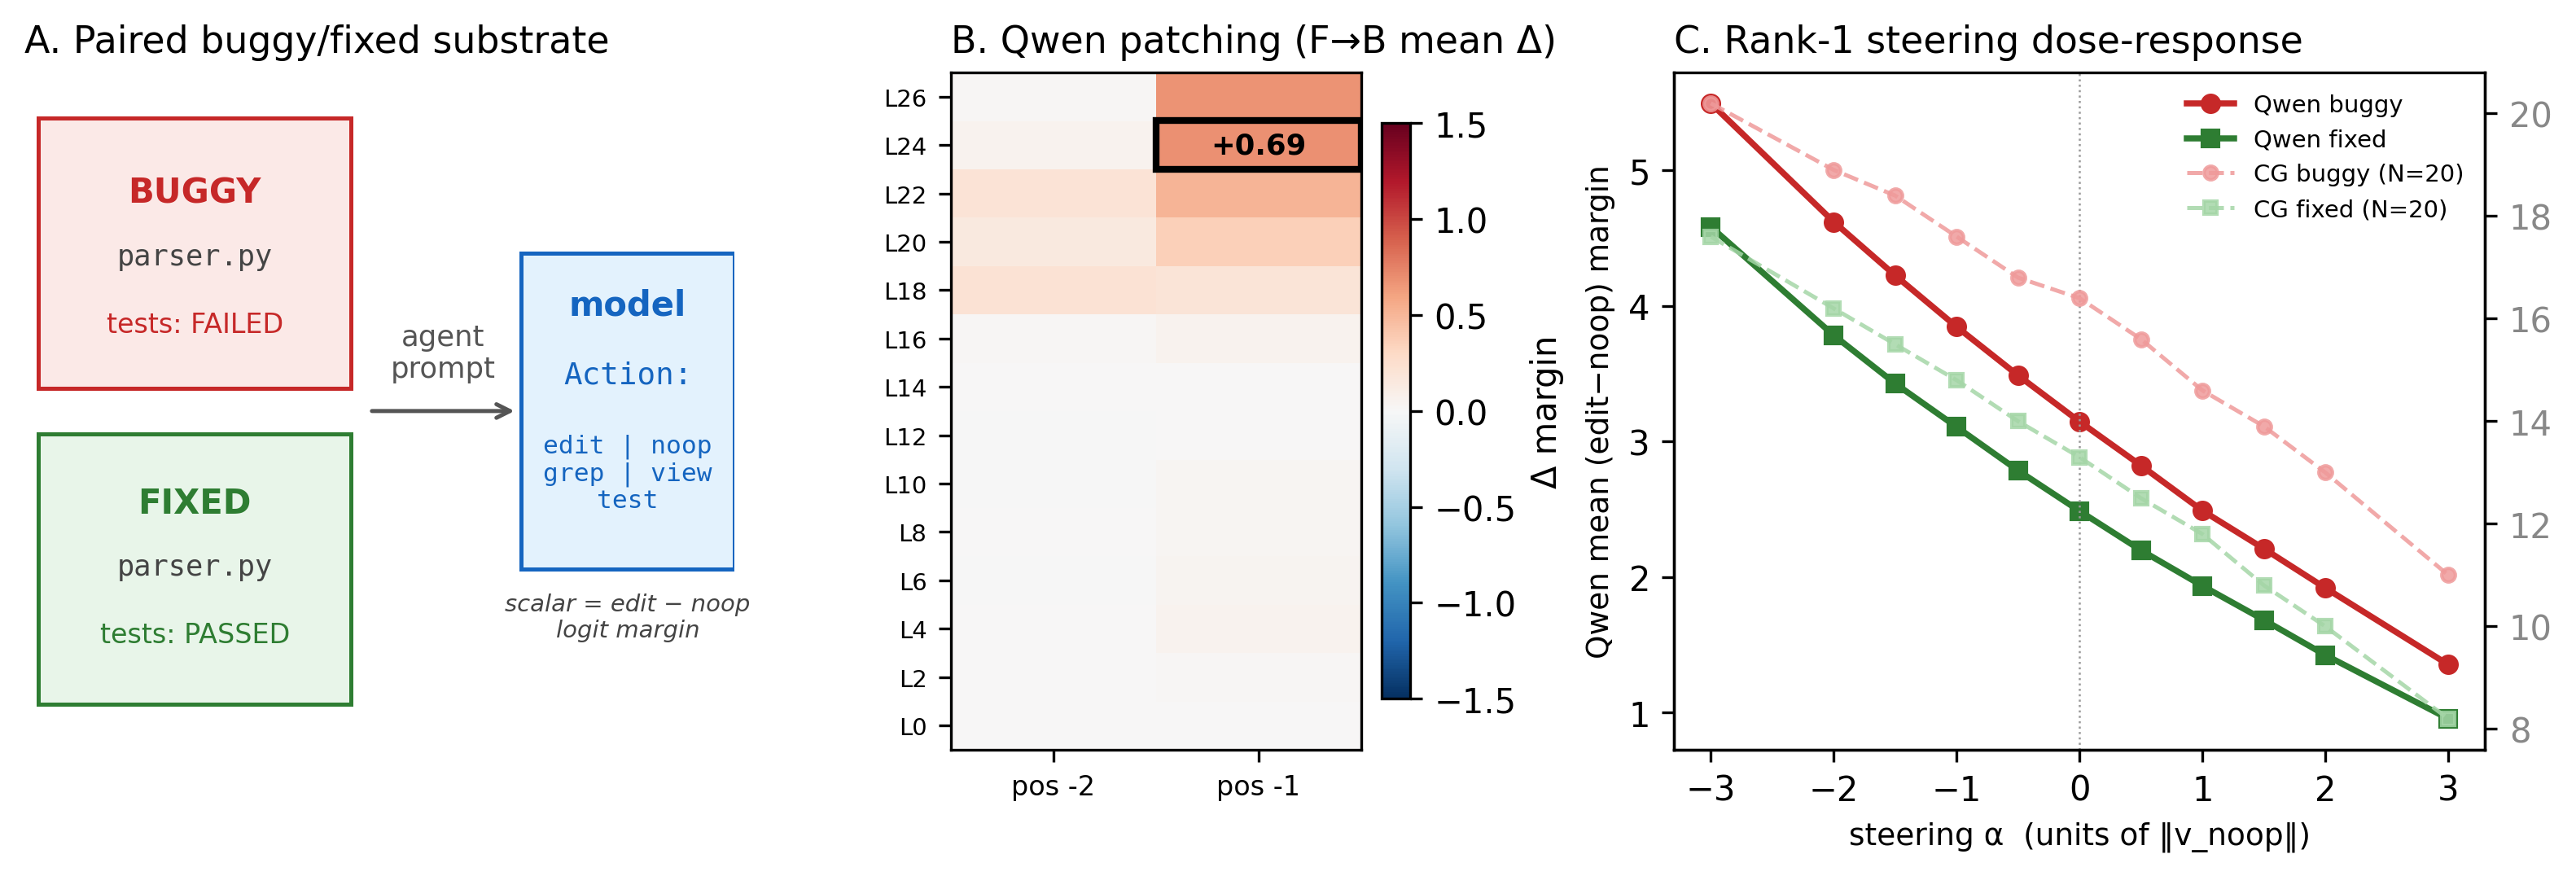
\includegraphics[width=0.99\linewidth,height=\textheight,keepaspectratio,alt={Qwen causal localization and steering. (A) Paired buggy/fixed toy substrate. (B) F\ensuremath{\rightarrow}B residual patching peaks at L24/pos \ensuremath{-}1 on the edit \ensuremath{-} noop margin. (C) Rank-1 steering along the toy fixed-minus-buggy contrast direction reproduces the margin shift. CodeGemma steering is shown only as a responsive-subset comparison; Qwen is the fully localized result. Panels (B)--(C) establish the available and causally read out steps of the represented-evidence-vs-action gap; the final action does not change at 1.5B's natural operating point (0\% noop; steering flips it, \S{}5.8).}]{figures/main_mechanism.png}
\caption{\textbf{Qwen causal localization and steering.} \emph{(A)}
Paired buggy/fixed toy substrate. \emph{(B)} F\ensuremath{\rightarrow}B residual patching peaks
at L24/pos \ensuremath{-}1 on the \protect\texttt{edit\ \ensuremath{-}\ noop} margin. \emph{(C)}
Rank-1 steering along the toy fixed-minus-buggy contrast direction
reproduces the margin shift. CodeGemma steering is shown only as a
responsive-subset comparison; Qwen is the fully localized result. Panels
(B)--(C) establish the \emph{available} and \emph{causally read out}
steps of the represented-evidence-vs-action gap; the final action does
not change at 1.5B's natural operating point (0\% \protect\texttt{noop};
steering flips it, \S{}5.8).}\label{fig:mechanism}
\end{figure}

\subsection{Scaling the causal mechanism across the Qwen family
(1.5B--32B)}\label{scaling-the-causal-mechanism-across-the-qwen-family-1.5b32b}

We extend the \S{}4.1 localization from 1.5B to the full
Qwen2.5-Coder-Instruct ladder, 1.5B, 3B, 7B, 14B, 32B, holding the
49-toy and 499-SWE substrates, the tokenizer, the chat template, and the
five-action menu fixed, so the \emph{only} variable across runs is the
forward pass (all five action names remain single-token at every size;
\S{}\ref{sec:tok-audit}). Per size we run paired bidirectional residual
patching on the 49 toy \texttt{code\_tests} pairs (coarse layer-step
2--4, plus a fine layer-step-1 sweep on 7B) and take the peak as the
cell maximizing the bidirectional minimum
\(\min(\text{F}\!\to\!\text{B},
\text{B}\!\to\!\text{F})\) on the \texttt{edit\ \ensuremath{-}\ noop} margin.

\textbf{A causally-used pass/fail readout exists at every scale.} The
peak is at the action position (pos \ensuremath{-}1), in the late layers,
bidirectionally significant (Wilcoxon one-sided \(p<10^{-9}\) on the 49
per-task F\ensuremath{\rightarrow}B effects), and bootstrap-stable (the peak layer is recovered
in 92--100\% of task resamples) at every size:

{\def\LTcaptype{none} % do not increment counter
\begin{longtable}[]{@{}
  >{\raggedright\arraybackslash}p{(\linewidth - 12\tabcolsep) * \real{0.1200}}
  >{\raggedleft\arraybackslash}p{(\linewidth - 12\tabcolsep) * \real{0.1600}}
  >{\raggedright\arraybackslash}p{(\linewidth - 12\tabcolsep) * \real{0.1200}}
  >{\raggedleft\arraybackslash}p{(\linewidth - 12\tabcolsep) * \real{0.1600}}
  >{\raggedright\arraybackslash}p{(\linewidth - 12\tabcolsep) * \real{0.1200}}
  >{\raggedleft\arraybackslash}p{(\linewidth - 12\tabcolsep) * \real{0.1600}}
  >{\raggedleft\arraybackslash}p{(\linewidth - 12\tabcolsep) * \real{0.1600}}@{}}
\toprule\noalign{}
\begin{minipage}[b]{\linewidth}\raggedright
size
\end{minipage} & \begin{minipage}[b]{\linewidth}\raggedleft
layers
\end{minipage} & \begin{minipage}[b]{\linewidth}\raggedright
peak (pos \ensuremath{-}1)
\end{minipage} & \begin{minipage}[b]{\linewidth}\raggedleft
rel.~depth
\end{minipage} & \begin{minipage}[b]{\linewidth}\raggedright
F\ensuremath{\rightarrow}B {[}95\% CI{]}
\end{minipage} & \begin{minipage}[b]{\linewidth}\raggedleft
toy B\ensuremath{-}F gap
\end{minipage} & \begin{minipage}[b]{\linewidth}\raggedleft
Wilcoxon \(p\)
\end{minipage} \\
\midrule\noalign{}
\endhead
\bottomrule\noalign{}
\endlastfoot
1.5B & 28 & L24 & 0.857 & \(+0.65\) & \(+0.66\) & (paper) \\
3B & 36 & L32 & 0.889 & \(+1.00\,[+0.86,+1.15]\) & \(+1.25\) &
\(<10^{-9}\) \\
7B & 28 & L27 (fine) & 0.964 & \(+2.77\) & \(+2.76\) & \(<10^{-9}\) \\
14B & 48 & L44 & 0.917 & \(+4.09\,[+3.53,+4.66]\) & \(+4.89\) &
\(<10^{-9}\) \\
32B & 64 & L60 & 0.938 & \(+11.66\,[+11.07,+12.25]\) & \(+14.14\) &
\(<10^{-9}\) \\
\end{longtable}
}

The 7B peak is from a fine layer-step-1 sweep (L18--27); the coarse
step-2 grid undershot at L26/0.929. The \texttt{code}-variant negative
control shows no peak at every size, as at 1.5B, so the site is
transcript-conditional.

\textbf{A relative-depth law that drifts deeper, and width, not just
depth, pushes it deeper.} The peaks sit at relative depth
0.857/0.889/0.964/0.917/0.938 (1.5B\ensuremath{\rightarrow}32B), a late-layer band that creeps
toward the final layer with size. The cleanest test is the 7B
\textbf{width control}: 7B has the \emph{same 28 layers} as 1.5B but
\textasciitilde2.3\ensuremath{\times} the width, and a fine layer-step-1 sweep (L18--27)
shows its F\ensuremath{\rightarrow}B effect rising monotonically to the \textbf{final layer}
(L27, relative depth 0.964, \(+2.77\) logits), far deeper than 1.5B's
L24 (0.857). The readout's location is therefore not a pure function of
relative depth; added width defers it toward the network's end. (Coarse
grids undershoot the exact layer, so the 3B/14B/32B peaks are likely a
touch deeper than reported.)

\textbf{Causal effect grows \textasciitilde18\ensuremath{\times} with scale.} The peak F\ensuremath{\rightarrow}B
shift grows monotonically from \(+0.65\) logits (1.5B) to \(+11.7\)
(32B), recovering \textasciitilde80--100\% of the toy buggy--fixed gap
at the coarse peak. The mechanism becomes far more behaviorally salient
with size.

\textbf{Discriminability \(\neq\) causal use, and the gap grows.} A
per-layer monitor scan on 3B (each layer's own toy contrast direction
projected onto the 499 SWE residuals) peaks at L27 (ROC-AUC 0.977), as
separable as 1.5B's best, while the \emph{causal} cell L32 reads only
0.867; the gap between the max-AUC layer and the causal-use layer is
\(+0.110\) at 3B vs \textasciitilde0.01 at 1.5B. Discriminative AUC does
not localize the mechanism (\S{}5.1), and that divergence widens with
scale.

\begin{figure}
\centering
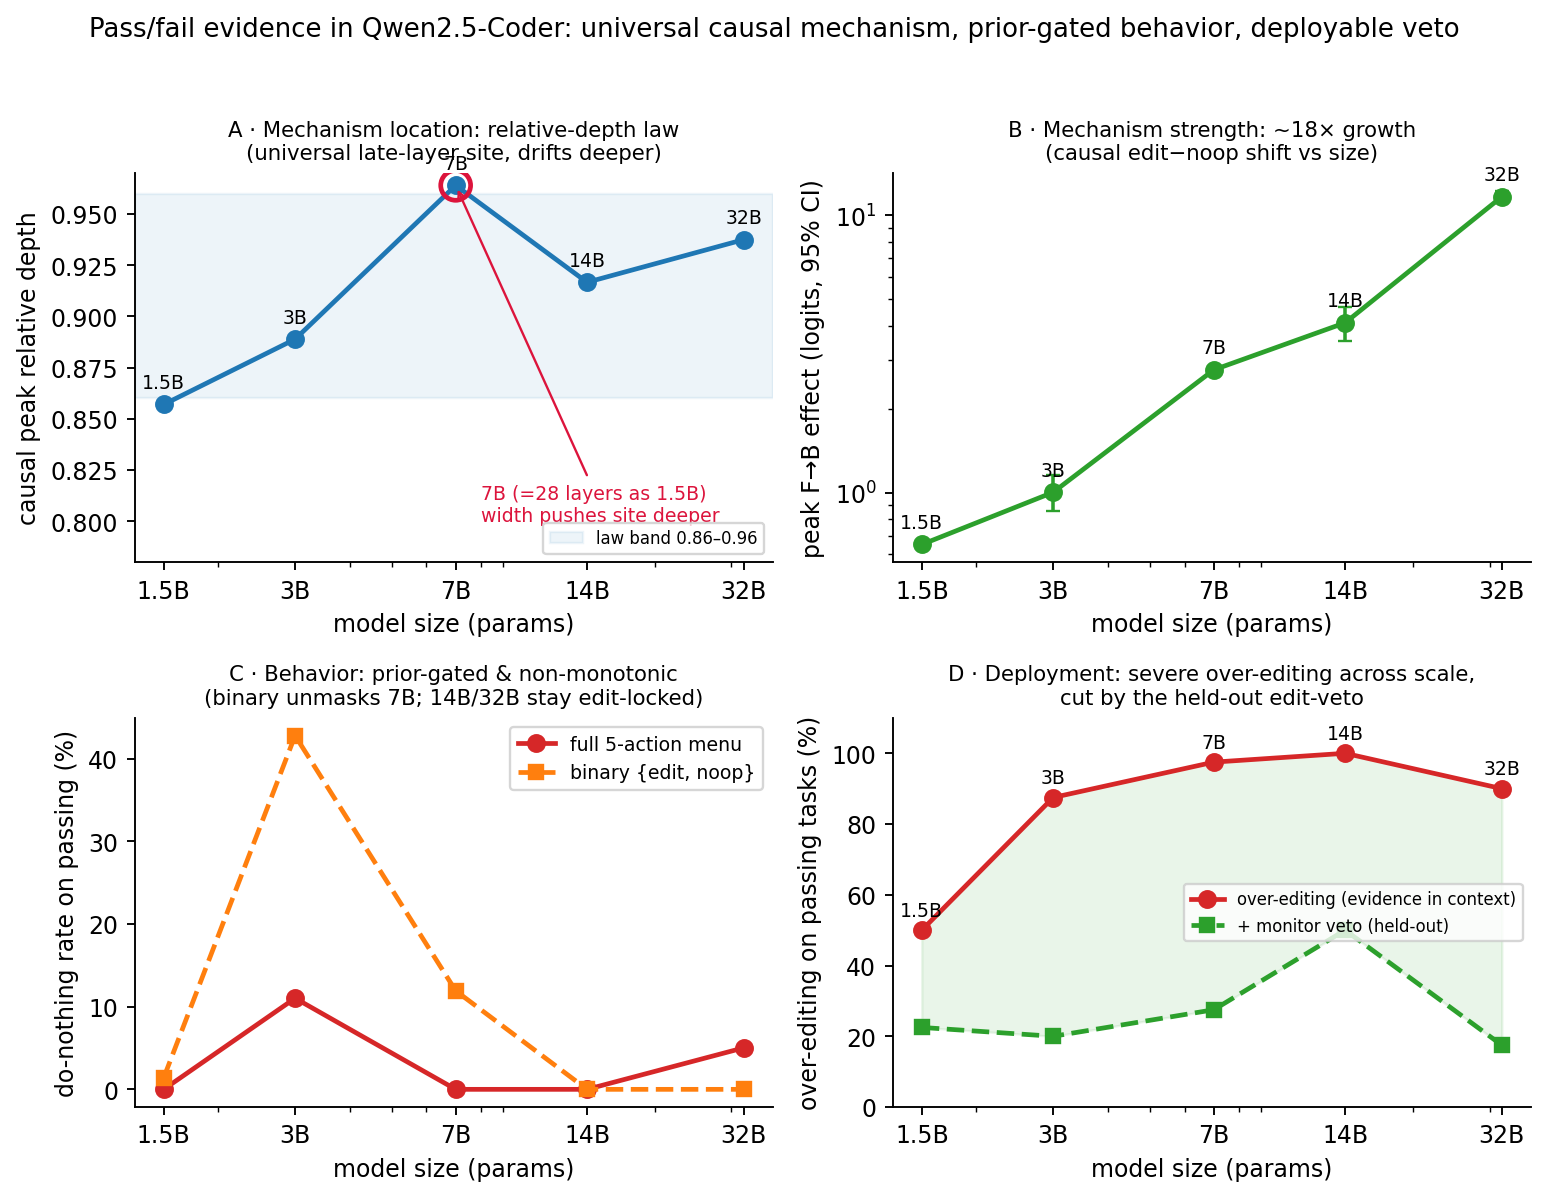
\includegraphics[width=0.99\linewidth,height=\textheight,keepaspectratio,alt={Scaling synthesis (Qwen2.5-Coder). (A) The causal readout's relative depth follows a late-layer law that drifts deeper with size; the 7B width control (fine-swept) peaks at the final layer. (B) The peak causal edit \ensuremath{-} noop effect grows \textasciitilde18\ensuremath{\times} (95\% CIs). (C) The do-nothing rate on passing prompts is non-monotonic and prior-gated; a binary \{edit, noop\} menu unmasks abstention for the view-prior 7B. (D) In a live agent loop, over-editing of already-passing code is severe across scale and is cut by a held-out monitor edit-veto.}]{figures/scaling_synthesis.png}
\caption{\textbf{Scaling synthesis (Qwen2.5-Coder).} \emph{(A)} The
causal readout's relative depth follows a late-layer law that drifts
deeper with size; the 7B width control (fine-swept) peaks at the final
layer. \emph{(B)} The peak causal \protect\texttt{edit\ \ensuremath{-}\ noop} effect
grows \textasciitilde18\ensuremath{\times} (95\% CIs). \emph{(C)} The do-nothing rate on
passing prompts is non-monotonic and prior-gated; a binary \{edit,
noop\} menu unmasks abstention for the view-prior 7B. \emph{(D)} In a
live agent loop, over-editing of already-passing code is severe across
scale and is cut by a held-out monitor edit-veto.}\label{fig:scaling}
\end{figure}

\section{From a Static Monitor to What It Actually
Reads}\label{from-a-static-monitor-to-what-it-actually-reads}

The \texttt{stale\_misleading} and \texttt{stale\_flaky} variants probe
what happens when evidence disagrees with itself (Qwen, N = 49 each):

{\def\LTcaptype{none} % do not increment counter
\begin{longtable}[]{@{}
  >{\raggedright\arraybackslash}p{(\linewidth - 8\tabcolsep) * \real{0.2410}}
  >{\raggedright\arraybackslash}p{(\linewidth - 8\tabcolsep) * \real{0.1807}}
  >{\raggedright\arraybackslash}p{(\linewidth - 8\tabcolsep) * \real{0.1928}}
  >{\raggedright\arraybackslash}p{(\linewidth - 8\tabcolsep) * \real{0.1928}}
  >{\raggedright\arraybackslash}p{(\linewidth - 8\tabcolsep) * \real{0.1928}}@{}}
\toprule\noalign{}
\begin{minipage}[b]{\linewidth}\raggedright
variant
\end{minipage} & \begin{minipage}[b]{\linewidth}\raggedright
argmax = edit
\end{minipage} & \begin{minipage}[b]{\linewidth}\raggedright
argmax = noop
\end{minipage} & \begin{minipage}[b]{\linewidth}\raggedright
argmax = grep
\end{minipage} & \begin{minipage}[b]{\linewidth}\raggedright
projection \(p=h\cdot u_{\rm tx}\) (lower=failing)
\end{minipage} \\
\midrule\noalign{}
\endhead
\bottomrule\noalign{}
\endlastfoot
stale\_misleading & 8.2\% & \textbf{0.0\%} & 91.8\% & \ensuremath{-}1.22 \\
stale\_flaky & 6.1\% & \textbf{0.0\%} & 93.9\% & \ensuremath{-}2.81 \\
(clean buggy) & 29\% & -- & -- & \ensuremath{-}5.53 \\
(clean fixed) & 41\% & -- & -- & +0.36 \\
\end{longtable}
}

These argmax percentages should not be read as monotonic in the
\texttt{edit\ \ensuremath{-}\ noop} submargin: Qwen's first-token action prior over
\texttt{grep}/\texttt{edit}/\texttt{noop} can shift argmax rates even
when the margin and projection move in the expected pass/fail-transcript
direction.

\textbf{The 0\% explicit-\texttt{noop} rate under this prompt format.}
Across 98 stale-evidence prompts the model never commits to explicit
abstention at first-token argmax; it defaults to \texttt{grep}
\textgreater90\% of the time. The \(u_{\rm tx}\) projection sits between
the clean-buggy and clean-fixed baselines; the residual direction tracks
the pass/fail-test evidence even when the emitted action does not (\S{}5.2
establishes that the residual direction is specifically tracking
transcript text, not a separately-encoded no-edit decision).

\textbf{Two confounds bound the 0\% number.} (a) \emph{Content-prior},
``the model specifically avoids the literal token \texttt{noop}.'' Ruled
out by App. G.7: swapping \texttt{noop} \ensuremath{\rightarrow} \texttt{done} or \texttt{skip}
preserves the 0.0\% abstention rate on all 499 Qwen prompts. (b)
\emph{Position-prior}, ``the model assigns lower probability to the
last-listed action.'' Addressed by the position-balanced and binary
controls in \S{}5.5: on Qwen and CodeGemma, \texttt{noop} stays essentially
never-selected at every named-menu position, so the 0\% canonical rate
is not primarily a last-position artifact for those two models. DeepSeek
differs under a single-token rerun, where the abstention label is
selected when listed first and nearly never otherwise; DeepSeek
action-level claims are therefore treated separately. These controls do
not turn first-token argmax into live-agent abstention behavior. A
thresholded projection can be used as a toy transcript-label flag in
this static prompt format, but App. G.8/G.10 show that direct transcript
parsing dominates it on clean transcripts; Appendix F contains the LOOCV
toy-monitor ROC at AUC = 1.000 in that setting.

\subsection{Generalization to SWE-bench-Verified-derived paired
prompts}\label{generalization-to-swe-bench-verified-derived-paired-prompts}

We evaluate the \textbf{same frozen unit monitor direction}
\(u_{\rm tx}\) (legacy artifact name \texttt{v\_noop}), computed once on
the toy tasks, never retrained, on \textbf{499/497/499 paired prompts
derived from SWE-bench Verified} (Qwen / CodeGemma / DeepSeek; Qwen and
DeepSeek use all 499 base pairs, while CodeGemma uses 497 after two
\textbf{2400-token-cap drops} to avoid A10G OOM on the 7B model). The
base set comes from the 500-instance Verified split with one instance
dropped at ingestion because its modified file was unavailable at the
base commit (file 404; full ingestion accounting in App. G.1). Each
prompt is constructed by extracting an 80-line oracle window around each
gold patch's largest Python hunk and synthesizing a pytest transcript
matching the buggy/fixed condition. \textbf{This is not an end-to-end
SWE-bench evaluation}: the agent is not given the repository, it does
not propose patches, and tests are not executed (the transcript text is
synthesized from FAIL\_TO\_PASS / PASS\_TO\_PASS metadata). It is a
static classifier evaluation on paired prompts that contain
test-pass/fail evidence, on the same prompt format used for the toy
substrate.

{\def\LTcaptype{none} % do not increment counter
\begin{longtable}[]{@{}
  >{\raggedright\arraybackslash}p{(\linewidth - 6\tabcolsep) * \real{0.2500}}
  >{\raggedright\arraybackslash}p{(\linewidth - 6\tabcolsep) * \real{0.2500}}
  >{\raggedright\arraybackslash}p{(\linewidth - 6\tabcolsep) * \real{0.2500}}
  >{\raggedright\arraybackslash}p{(\linewidth - 6\tabcolsep) * \real{0.2500}}@{}}
\toprule\noalign{}
\begin{minipage}[b]{\linewidth}\raggedright
metric
\end{minipage} & \begin{minipage}[b]{\linewidth}\raggedright
Qwen-1.5B
\end{minipage} & \begin{minipage}[b]{\linewidth}\raggedright
CodeGemma-7B
\end{minipage} & \begin{minipage}[b]{\linewidth}\raggedright
DeepSeek-1.3B
\end{minipage} \\
\midrule\noalign{}
\endhead
\bottomrule\noalign{}
\endlastfoot
ROC-AUC {[}95\% CI{]} & \textbf{0.989} {[}0.983, 0.994{]} &
\textbf{0.950} {[}0.938, 0.961{]} & \textbf{0.888} {[}0.866, 0.907{]} \\
AP {[}95\% CI{]} & 0.991 {[}0.986, 0.994{]} & 0.949 {[}0.935, 0.961{]} &
0.879 {[}0.851, 0.906{]} \\
precision (in-sample thr.) & 0.973 (468/481) & 0.894 (438/490) & 0.809
(414/512) \\
recall (in-sample thr.) & 0.938 (468/499) & 0.881 (438/497) & 0.830
(414/499) \\
fixed-condition FPR (in-sample thr.) & 0.026 (13/499) & 0.105 (52/497) &
0.196 (98/499) \\
\end{longtable}
}

CodeGemma uses the all-49 toy contrast at (L26, pos \ensuremath{-}1) in all headline
monitor results; the 20-task responsive subset is retained only for
steering and exploratory SAE analyses (App. G.4, H.6).

The positive class is the matched failing-transcript / buggy condition
(N = 499/497/499); the negative class is the matched passing-transcript
/ fixed condition (same N). The fixed-condition FPR row counts
fixed/passing-transcript prompts whose classifier score
\(s=-h\cdot u_{\rm tx}\) exceeds the threshold. It is a classifier
false-positive rate, not an observed committed edit action. AUC and AP
CIs are paired-bootstrap (B = 10000, seed = 0) over the full per-task
score vector (reproduction in App. J). \textbf{The bottom three rows use
the balanced-accuracy threshold chosen on each model-specific evaluation
set (499/497/499 for Qwen/CodeGemma/DeepSeek)} and are therefore
\emph{in-sample}; they are deployment-illustrative, not out-of-sample
estimates, and we report them in lower contrast than the threshold-free
AUC/AP rows. Held-out threshold checks for Qwen are documented in App.
G.5 (50/50 split + leave-one-repo-out). The App. G.10 single-turn veto
simulation uses the Qwen held-out 50/50 mean threshold, a computed
DeepSeek held-out 50/50 mean threshold, and the CodeGemma in-sample
balanced-accuracy threshold under the all-49 direction (artifacts in
App. J). \textbf{Formal held-out canonical-menu calibration tables for
CodeGemma and DeepSeek remain future work} (the raw \S{}5.1 per-task
projection caches are not retained, so reproducing them needs model
forwards); App. G.17 does report a cross-model held-out operating point
in the disjoint-template paraphrase setting (threshold frozen on train
templates). App. G.3 documents per-repo calibration on CodeGemma in
detail.

\textbf{The discriminative pass/fail-transcript signal is broadly
separable across layers; causal usage is localized by patching, not
AUC.} On the 499-prompt evaluation, projecting \(u_{\rm tx}\) at the
\emph{wrong} layer (L12) and same position gives AUC \textbf{0.998},
\emph{higher} than the L24 monitor's 0.989; the wrong- \emph{position}
control (L24 / pos \ensuremath{-}8) drops substantially to 0.707; PCA1 at (L24, pos
\ensuremath{-}1) gives 0.977 (Adversarial table, App. G.2). Two implications: (i)
discriminative AUC by itself does not localize the mechanism, the
pass/fail-transcript evidence is linearly readable along similar
directions across many layers, and the choice of (L24, pos \ensuremath{-}1) is
justified by causal patching (\S{}4.1), not by the projection's
discriminative power; (ii) the projection is plausibly reading features
that correlate strongly with explicit pass/fail transcript text, a
hypothesis we resolve in \S{}5.2.

Each model uses a different argmax-action hedge, Qwen \texttt{grep}
90\%/83\% buggy/fixed, CodeGemma \texttt{edit} \ensuremath{\approx}99\% in both, DeepSeek
\texttt{view} 78\%/85\%, but the explicit-\texttt{noop} rate at
first-token argmax is \textbf{0\%} across the 499/497/499 prompts (exact
for Qwen and CodeGemma; a first-subword proxy for DeepSeek, whose
canonical \texttt{noop} is multi-token, \S{}\ref{sec:tok-audit}), while the
monitor's projection cleanly separates the conditions (gaps +4.73 Qwen,
+2.87 CodeGemma, +5.64 DeepSeek). On these static prompts the residual
direction tracks the pass/fail-transcript evidence even though the
emitted action does not pick \texttt{noop}; note that the action
distribution shifts (Qwen's \texttt{edit} rate drops slightly on fixed
prompts vs buggy, App. G.1) but a much larger first-token prior favors
\texttt{grep} / \texttt{edit} / \texttt{view} over the abstention token.
The evidence affects the \texttt{edit\ \ensuremath{-}\ noop} submargin without
overcoming this action prior. Whether a \emph{monitor-mediated agent} in
an in-the-loop setting would convert the submargin shift into fewer
spurious edits at acceptable recall is taken up by the agent-loop
edit-veto in \S{}5.9. Monitor-direction baselines, the per-repo regression
analysis driving CodeGemma's 10.5\% in-sample fixed-condition FPR
(concentrated in \texttt{django/django} at 13.0\% and
\texttt{sphinx-doc/sphinx} at 22.7\%), a per-repo calibration
counterfactual that drops the pooled in-sample fixed-condition FPR to
9.3\%, and a sample-efficiency sweep showing that \(u_{\rm tx}\) derived
from only 10 toy paired tasks is within 0.001 AUC of the full-49
baseline (\S{}G.4) are in Appendix G.

\begin{figure}
\centering
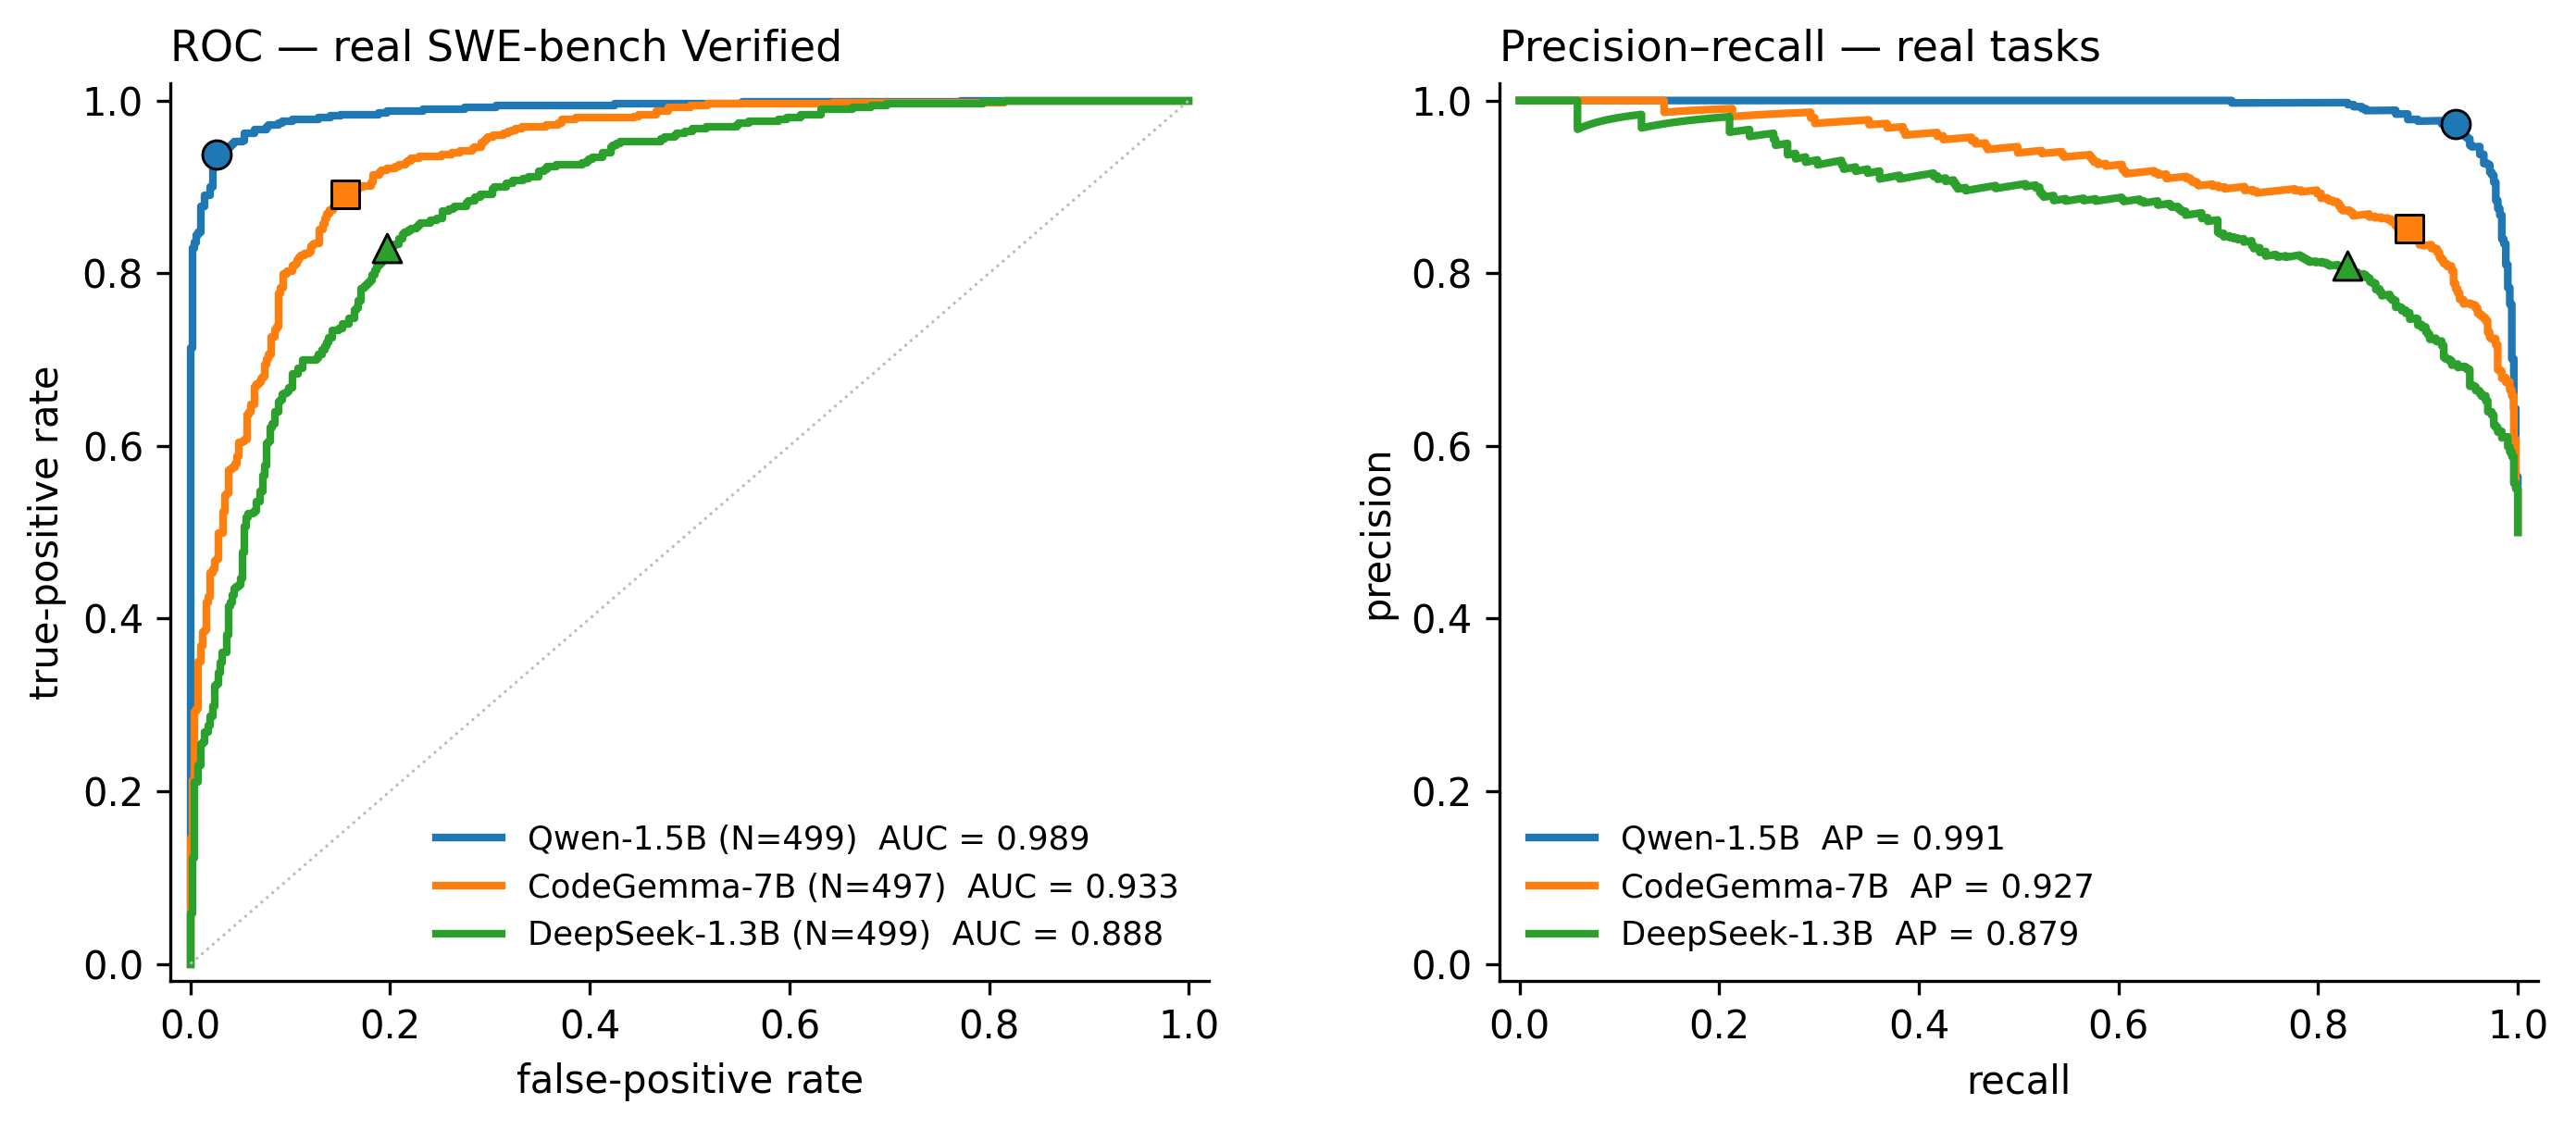
\includegraphics[width=0.98\linewidth,height=\textheight,keepaspectratio,alt={Projection monitor on SWE-bench-Verified-derived paired prompts. A frozen one-dot-product monitor at the Qwen causal site, or each other model's reported action-position cell, separates failing-transcript from passing-transcript prompts (AUC 0.989/0.950/0.888 for Qwen/CodeGemma/DeepSeek; full metrics in the \S{}5.1 table). Threshold markers are in-sample operating points and are illustrative only. This is a static-prompt classifier evaluation, not an end-to-end SWE-bench agent run.}]{figures/main_monitor.png}
\caption{\textbf{Projection monitor on SWE-bench-Verified-derived paired
prompts.} A frozen one-dot-product monitor at the Qwen causal site, or
each other model's reported action-position cell, separates
failing-transcript from passing-transcript prompts (AUC
0.989/0.950/0.888 for Qwen/CodeGemma/DeepSeek; full metrics in the \S{}5.1
table). Threshold markers are in-sample operating points and are
illustrative only. This is a static-prompt classifier evaluation, not an
end-to-end SWE-bench agent run.}\label{fig:monitor}
\end{figure}

\subsection{Contradictory-transcript control: what the projection
actually
reads}\label{contradictory-transcript-control-what-the-projection-actually-reads}

The \S{}5.1 0.989 AUC has an obvious alternative explanation: the
synthesized pytest transcripts contain explicit lexical markers
(\texttt{FAILED\ test\_x\ ...\ AssertionError} in buggy,
\texttt{N\ passed\ in\ 0.04s} in fixed; App. G.1). A direction that
separates buggy from fixed prompts might therefore be reading the
\textbf{transcript text} rather than the code's correctness. We resolve
this with a 2 \ensuremath{\times} 2 (code \ensuremath{\times} transcript) contradictory-transcript control
on Qwen, run on the same 499 paired prompts, and run the same control on
CodeGemma and DeepSeek (cross-model table below).

\textbf{Design.} For each task we materialize four prompts (variant
\texttt{code\_tests\_swapped} in
\texttt{src/no\_op\_circuit/dataset/schema.py}):

{\def\LTcaptype{none} % do not increment counter
\begin{longtable}[]{@{}
  >{\raggedright\arraybackslash}p{(\linewidth - 6\tabcolsep) * \real{0.0930}}
  >{\raggedright\arraybackslash}p{(\linewidth - 6\tabcolsep) * \real{0.1395}}
  >{\raggedright\arraybackslash}p{(\linewidth - 6\tabcolsep) * \real{0.2326}}
  >{\raggedright\arraybackslash}p{(\linewidth - 6\tabcolsep) * \real{0.5349}}@{}}
\toprule\noalign{}
\begin{minipage}[b]{\linewidth}\raggedright
code
\end{minipage} & \begin{minipage}[b]{\linewidth}\raggedright
transcript
\end{minipage} & \begin{minipage}[b]{\linewidth}\raggedright
label
\end{minipage} & \begin{minipage}[b]{\linewidth}\raggedright
source
\end{minipage} \\
\midrule\noalign{}
\endhead
\bottomrule\noalign{}
\endlastfoot
buggy & failing & (B,B), matched & original \S{}5.1 prompts \\
fixed & passing & (F,F), matched & original \S{}5.1 prompts \\
buggy & passing & (B,F), swapped & new
\texttt{buggy\_\_code\_tests\_swapped.pt} \\
fixed & failing & (F,B), swapped & new
\texttt{fixed\_\_code\_tests\_swapped.pt} \\
\end{longtable}
}

Both swapped cells reuse the \emph{paired-task's own} opposite-condition
transcript verbatim, so transcript-text format is constant across cells.
Each prompt is scored with the \textbf{frozen} toy-trained
\(u_{\rm tx}\) at L24/pos \ensuremath{-}1; score \(s=-p\) per \S{}5.1.

\textbf{Result.} Cell means and bootstrap (B = 10 000, seed = 0)
decomposition over the N = 499 paired tasks (Qwen-1.5B):

{\def\LTcaptype{none} % do not increment counter
\begin{longtable}[]{@{}llrl@{}}
\toprule\noalign{}
code & transcript & mean score & interpretation \\
\midrule\noalign{}
\endhead
\bottomrule\noalign{}
\endlastfoot
buggy & failing & \textbf{+2.18} & matched (B,B), high \\
fixed & failing & \textbf{+2.17} & swapped (F,B), high \\
buggy & passing & \textbf{\ensuremath{-}2.56} & swapped (B,F), low \\
fixed & passing & \textbf{\ensuremath{-}2.56} & matched (F,F), low \\
\end{longtable}
}

{\def\LTcaptype{none} % do not increment counter
\begin{longtable}[]{@{}
  >{\raggedright\arraybackslash}p{(\linewidth - 4\tabcolsep) * \real{0.4333}}
  >{\raggedleft\arraybackslash}p{(\linewidth - 4\tabcolsep) * \real{0.1833}}
  >{\raggedright\arraybackslash}p{(\linewidth - 4\tabcolsep) * \real{0.3833}}@{}}
\toprule\noalign{}
\begin{minipage}[b]{\linewidth}\raggedright
main effect
\end{minipage} & \begin{minipage}[b]{\linewidth}\raggedleft
value
\end{minipage} & \begin{minipage}[b]{\linewidth}\raggedright
95\% CI
\end{minipage} \\
\midrule\noalign{}
\endhead
\bottomrule\noalign{}
\endlastfoot
\textbf{\ensuremath{\Delta}Transcript} (failing \ensuremath{-} passing, averaged over code) &
\textbf{+4.733} & {[}+4.606, +4.862{]} \\
\textbf{\ensuremath{\Delta}Code} (buggy \ensuremath{-} fixed, averaged over transcript) &
\textbf{+0.002} & {[}\ensuremath{-}0.025, +0.029{]} \\
Interaction & +0.002 & {[}\ensuremath{-}0.010, +0.014{]} \\
\end{longtable}
}

The transcript effect is large; the code effect is statistically
indistinguishable from zero (CI crosses 0 on N = 499 paired tasks). As
threshold-free metrics on the swapped off-diagonal (998 prompts):

{\def\LTcaptype{none} % do not increment counter
\begin{longtable}[]{@{}
  >{\raggedright\arraybackslash}p{(\linewidth - 4\tabcolsep) * \real{0.3294}}
  >{\raggedleft\arraybackslash}p{(\linewidth - 4\tabcolsep) * \real{0.1294}}
  >{\raggedright\arraybackslash}p{(\linewidth - 4\tabcolsep) * \real{0.5412}}@{}}
\toprule\noalign{}
\begin{minipage}[b]{\linewidth}\raggedright
labeling (positive class)
\end{minipage} & \begin{minipage}[b]{\linewidth}\raggedleft
ROC-AUC
\end{minipage} & \begin{minipage}[b]{\linewidth}\raggedright
meaning
\end{minipage} \\
\midrule\noalign{}
\endhead
\bottomrule\noalign{}
\endlastfoot
\textbf{transcript = failing} & \textbf{0.988} & direction follows
transcript text \\
\textbf{code = buggy} & \textbf{0.012} & anti-aligned with the code
label: the direction tracks the (swapped) transcript, not the underlying
code-semantics label (0.012 = 1 \ensuremath{-} 0.988, the same ordering scored
against the inverted label) \\
\end{longtable}
}

\textbf{Verdict.} On 499 SWE-bench-Verified-derived static paired
prompts, the \(u_{\rm tx}\) direction tracks \textbf{pass/fail
transcript text}, not code semantics. The \S{}5.1 AUC of 0.989 is
essentially the transcript-label AUC of 0.988 measured here; the +0.001
gap is sampling noise. The \S{}1 framing ``carries the pass/fail-test
transcript evidence the model is given'' should be read narrowly: the
\emph{evidence} in question is the pytest transcript text, not the
underlying code correctness. Three implications:

\begin{itemize}
\tightlist
\item
  \textbf{The \S{}5.1 monitor is a pass/fail-transcript-text classifier.}
  Anything an external system could compute by directly parsing the
  pytest transcript (e.g.~a regex for \texttt{FAILED} / \texttt{passed};
  App. G.8 reports such a baseline at AUC \textbf{1.000}) the projection
  monitor reads more indirectly. The mechanistic value of this paper is
  in \emph{where} and \emph{how} that evidence is read out at an
  action-token residual-stream site, not in offering a better classifier
  than a regex.
\item
  \textbf{The mechanism story in \S{}4 is still empirically valid but
  narrower in interpretation.} The causal patching peak at (L24, pos \ensuremath{-}1)
  on Qwen is the site at which substituting one prompt's residual into
  another's forward shifts the \texttt{edit\ \ensuremath{-}\ noop} margin. The \S{}5.2
  result clarifies that the \emph{quantity being patched} is best
  understood as the residual carrier of pass/fail-test evidence at the
  action position, not a separately-encoded no-edit \emph{decision}.
  App. G.9 bounds the no-transcript case for the tested Qwen L24 linear
  readouts: frozen \(u_{\rm tx}\), a fresh contrastive direction, and a
  1536-D LR probe are all near chance (AUC \ensuremath{\leq} 0.52); the toy
  \texttt{code} variant also shows no patching peak (App. D).
\item
  \textbf{The SAE features (\S{}5.4, App. H) re-interpret as
  pass/fail-transcript features.} The OMP-selected top features whose
  logit-lens promotions are \texttt{error} / \texttt{traceback} /
  \texttt{already} / \texttt{passed} are exactly the features one would
  expect a SAE trained on these prompts to learn for representing
  pass/fail transcripts. They should therefore be interpreted as
  pass/fail-transcript features rather than no-op-circuit elements.
\end{itemize}

\textbf{Cross-model reported-cell evidence (CodeGemma + DeepSeek).} We
re-run the identical 2 \ensuremath{\times} 2 control on the other two models, scoring each
at its \S{}4.3 reported patch cell with its own frozen \(u_{\rm tx}\)
(CodeGemma L26, all-49 direction; DeepSeek L22), all four cells
forwarded fresh server-side (App. G.16). The transcript-driven verdict
holds on all three (raw \ensuremath{\Delta}Transcript magnitudes are in each model's own
projection scale and not directly comparable; the model-invariant
quantities are the \textbar \ensuremath{\Delta}Code\textbar/\textbar \ensuremath{\Delta}Transcript\textbar{}
ratio and the swapped-only AUCs):

{\def\LTcaptype{none} % do not increment counter
\begin{longtable}[]{@{}
  >{\raggedright\arraybackslash}p{(\linewidth - 6\tabcolsep) * \real{0.2155}}
  >{\raggedright\arraybackslash}p{(\linewidth - 6\tabcolsep) * \real{0.2241}}
  >{\raggedright\arraybackslash}p{(\linewidth - 6\tabcolsep) * \real{0.2328}}
  >{\raggedright\arraybackslash}p{(\linewidth - 6\tabcolsep) * \real{0.3276}}@{}}
\toprule\noalign{}
\begin{minipage}[b]{\linewidth}\raggedright
model (cell)
\end{minipage} & \begin{minipage}[b]{\linewidth}\raggedright
\ensuremath{\Delta}Transcript {[}95\% CI{]}
\end{minipage} & \begin{minipage}[b]{\linewidth}\raggedright
\ensuremath{\Delta}Code {[}95\% CI{]}
\end{minipage} & \begin{minipage}[b]{\linewidth}\raggedright
swapped-only AUC (transcript / code)
\end{minipage} \\
\midrule\noalign{}
\endhead
\bottomrule\noalign{}
\endlastfoot
Qwen-1.5B (L24, N=499) & \textbf{+4.733} {[}4.61, 4.86{]} & +0.002
{[}\ensuremath{-}0.025, +0.029{]} & \textbf{0.988} / 0.012 \\
CodeGemma-7B (L26, N=496) & \textbf{+2.894} {[}2.80, 2.99{]} & \ensuremath{-}0.046
{[}\ensuremath{-}0.080, \ensuremath{-}0.013{]} & \textbf{0.951} / 0.049 \\
DeepSeek-1.3B (L22, N=499) & \textbf{+5.697} {[}5.46, 5.94{]} & \ensuremath{-}0.053
{[}\ensuremath{-}0.168, +0.061{]} & \textbf{0.888} / 0.112 \\
\end{longtable}
}

On every model \textbar \ensuremath{\Delta}Code\textbar{} \ensuremath{\leq} 0.06 and
\textbar \ensuremath{\Delta}Code\textbar/\textbar \ensuremath{\Delta}Transcript\textbar{} \textless{} 0.02;
when code and transcript \textbf{contradict} within a single prompt, the
projection follows the transcript (AUC 0.89--0.99) and is inverted
against the code label (AUC 0.01--0.11), because in the swapped cells
the transcript label is anti-correlated with the code condition. \ensuremath{\Delta}Code's
CI crosses zero on Qwen and DeepSeek (a genuine null); on CodeGemma it
is a tiny but statistically non-zero \emph{negative} effect (\ensuremath{-}0.046,
\textasciitilde63\ensuremath{\times} smaller than \ensuremath{\Delta}Transcript), if anything the projection
very slightly anti-tracks code, the opposite of a code-driven reading.
The keystone ``reads transcript, not code'' control is therefore
\textbf{three-model}, not Qwen-only.

We are careful not to over-read this in the other direction either. The
\S{}4 causal patching site is real, the steering intervention is real, and
the projection is a meaningful mechanistic observable for the
pass/fail-transcript pathway. We do \textbf{not} claim the projection is
superior to direct transcript parsing; its value here is mechanistic: it
identifies where explicit pass/fail evidence is read out at an
action-token residual-stream site and shows that this evidence affects
the \texttt{edit\ \ensuremath{-}\ noop} margin despite not dominating the first-token
argmax.

Full analysis artifacts and scripts are listed in App. G.16.

\subsection{Temporal separation: the transcript verdict survives
upstream}\label{temporal-separation-the-transcript-verdict-survives-upstream}

\S{}5.2 establishes that the projection reads the transcript text. A
natural objection is that this is then \emph{trivial}: in every result
so far the transcript is the \textbf{last evidence block before the
\texttt{Action:} token}, so the direction may simply be reading a
\texttt{FAILED} token we inserted one block above the readout, exactly
what a \texttt{contains("FAILED")} regex does, and does better (App.
G.8, G.10). We test this by moving the transcript \textbf{upstream}.

We reformat each of the 499 SWE-derived prompts (Qwen) into a multi-turn
agent trace: turn 1 shows issue + code; turn 2 is an assistant
\texttt{test} action and turn 3 shows the \textbf{condition-matched
pytest transcript} used in \S{}5.1; then two \textbf{condition-neutral
intervening turns} (a \texttt{grep} with no matches and a generic file
view, byte-identical across buggy and fixed and across all tasks) push
the transcript upstream before the final \texttt{Action:} decision. The
decision-point's local context therefore contains \textbf{no pass/fail
tokens at all}. We score with the \emph{same frozen toy-trained unit
monitor direction \(u_{\rm tx}\)} at (L24, pos \ensuremath{-}1) used in \S{}5.1, no
retraining (full design + format control in App. G.15).

{\def\LTcaptype{none} % do not increment counter
\begin{longtable}[]{@{}
  >{\raggedright\arraybackslash}p{(\linewidth - 6\tabcolsep) * \real{0.2561}}
  >{\raggedleft\arraybackslash}p{(\linewidth - 6\tabcolsep) * \real{0.2439}}
  >{\raggedleft\arraybackslash}p{(\linewidth - 6\tabcolsep) * \real{0.2195}}
  >{\raggedleft\arraybackslash}p{(\linewidth - 6\tabcolsep) * \real{0.2805}}@{}}
\toprule\noalign{}
\begin{minipage}[b]{\linewidth}\raggedright
transcript position
\end{minipage} & \begin{minipage}[b]{\linewidth}\raggedleft
projection ROC-AUC
\end{minipage} & \begin{minipage}[b]{\linewidth}\raggedleft
turn-local regex
\end{minipage} & \begin{minipage}[b]{\linewidth}\raggedleft
full-scrollback regex
\end{minipage} \\
\midrule\noalign{}
\endhead
\bottomrule\noalign{}
\endlastfoot
adjacent (\S{}5.1) & 0.989 & 1.000 & 1.000 \\
\textbf{2 turns upstream (this \S{})} & \textbf{0.807} {[}0.788, 0.827{]} &
\textbf{0.500} & 1.000 \\
absent, format-matched control & 0.509 {[}0.494, 0.525{]} & 0.500 &
0.500 \\
\end{longtable}
}

Three things follow. \textbf{(i) The transcript verdict survives the
separation.} With the transcript two turns + the intervening tokens
upstream, the frozen direction still discriminates buggy from fixed at
\textbf{AUC 0.807}, degraded from the adjacent 0.989 (dilution is
expected) but far above both the format control (0.509, which holds
everything constant except the transcript and confirms the multi-turn
\emph{format} alone creates no discriminability) and the \S{}G.9
no-transcript floor. The direction \textbf{carries the transcript
verdict across intervening turns}, not a reading of an adjacent planted
token. \textbf{(ii) It beats a stateless turn-local regex (only).} A
stateless turn-local regex, one inspecting only the current observation
before the next action, reads chance (0.500), because the
\texttt{FAILED} token is two turns upstream. The residual carries the
transcript verdict to the decision point where a stateless local parser
sees nothing. This does \textbf{not} beat a full-history regex or a
stateful parser that records earlier test outcomes: both would recover
the upstream transcript (the full-scrollback regex is at 1.000 here).
The value is mechanistic, a carried-forward within-context
representation, not deployment superiority over text parsing.
\textbf{(iii) The action hides what the residual reveals.} In this
setting Qwen's first-token argmax is \emph{identical} across conditions
(buggy 173 \texttt{edit} / 326 \texttt{grep}; fixed 173 / 326), yet the
projection separates them at 0.807, the clearest demonstration in the
paper that the direction reads evidence the emitted behavior does not
surface, the same represented-evidence-versus-action gap behind the 0\%
noop result (\S{}5.1, \S{}4.2).

This is a single forward pass over a constructed multi-turn prompt, not
a live agent loop with KV-cache continuation across real turns;
``temporally separated'' here means positionally distant within one
context (the transcript is still textually present, hence the
full-scrollback regex still works). A genuinely \emph{evicted}
transcript is the \S{}G.9 no-transcript regime, which is negative. Full
design, the format-control variant, and server-side scoring are in App.
G.15.

\subsection{SAE decomposition (exploratory): pass/fail-transcript
features}\label{sae-decomposition-exploratory-passfail-transcript-features}

Exploratory SAE decomposition is reported in Appendix H (Fig.
\ref{fig:sae}). The contrast direction is geometrically dense in the
learned SAE basis, and small OMP-selected feature subsets can partially
affect the \texttt{edit\ \ensuremath{-}\ noop} margin, but the feature identities and
behavioral effects are seed-fragile and artifact-specific (a seed=0
re-run does not reproduce the exact magnitudes; App. H.7). In light of
\S{}5.2 the top features are best read as pass/fail-transcript features,
not ``no-op-circuit'' elements. We therefore do not treat the SAE
decomposition as a core contribution.

\subsection{Action-menu controls: near-zero abstention is
position-robust under named
menus}\label{action-menu-controls-near-zero-abstention-is-position-robust-under-named-menus}

The 0\% explicit-\texttt{noop} result (\S{}4) could be a list-position
artifact, since \texttt{noop} is always last in the canonical menu. We
re-score the 499 Qwen SWE-derived \texttt{code\_tests} paired prompts
under three menu manipulations; all five action names are single-token
under the Qwen tokenizer (scripts in App. J).

\textbf{Action order (position-balanced).} Across five cyclic orderings
that place \texttt{noop} in each menu slot exactly once (4,990 prompts),
\texttt{noop} is the argmax in \textbf{1/4,990} prompts, \ensuremath{\leq}0.1\% at every
position, with per-position 95\% bootstrap CIs upper-bounded at 0.3\%
(Fig. \ref{fig:action_order}). Menu order does shift the choice
\emph{among non-abstention actions} (when \texttt{noop} is first,
\texttt{edit} 68\% / \texttt{grep} 32\%; when \texttt{noop} is fourth,
\texttt{grep} 100\%) and modestly moves the \texttt{edit\ \ensuremath{-}\ noop}
margin (mean 0.95--2.40 logits by slot), but \texttt{noop} stays at mean
rank \ensuremath{\approx}4.7--5.0 of 5. The 0\% result is therefore not primarily a
position artifact under the named menu.

\textbf{Binary \texttt{edit}/\texttt{noop}.} Removing
\texttt{view}/\texttt{grep}/\texttt{test} does not unlock abstention:
\texttt{noop} is the argmax in 1.2\% (buggy) / 2.8\% (fixed) of prompts
when listed second and \textbf{0\%} when listed first (1,996 prompts).
So \texttt{grep}/\texttt{view} are not merely investigation hedges
concealing a latent preference to abstain; the edit prior dominates even
in a two-way choice. The small fixed \textgreater{} buggy gap (2.8\% vs
1.2\%) is consistent with the transcript mattering at the margin.

\textbf{Abstract labels (A--E).} Presented as letters with an in-prompt
mapping, first-token choice is dominated by a \emph{label-token} prior
rather than action meaning: Qwen emits \texttt{B} in 75\% of prompts
regardless of what \texttt{B} denotes (it emits \texttt{B} on 89\% of
the prompts where \texttt{B} is not \texttt{noop}). The apparent 21\%
``abstention'' when \texttt{noop} maps to \texttt{B} is this
\texttt{B}-prior, not a semantic decision (abstention near 0\% when
\texttt{noop} maps to A, C, D, or E). A content-free baseline confirms
an intrinsic surface-form prior: with the same A--E letters carrying
\textbf{no} action meaning, Qwen picks \texttt{B} on \textbf{97\%} of
998 prompts (the \texttt{letter\_only} control). Under abstract labels,
first-token choice is therefore governed largely by a letter prior, with
action meaning only a minor modulation.

Together, the named-menu and binary controls show the near-zero
\texttt{noop} selection is not primarily caused by \texttt{noop} being
last in the canonical menu (position-robust on Qwen and CodeGemma, and
surviving binarization). The abstract-label control, however, reveals
strong surface-form priors over letters, so first-token selection
remains heavily shaped by prompt-conditioned token preferences. We
therefore read this as a static prompt-conditioned action-token
preference, not live-agent abstention behavior, distinct from the
internal transcript-evidence representation of \S{}4--\S{}5.

\textbf{Cross-model.} On CodeGemma (action names single-token) the same
result holds: \texttt{noop} is argmax in \ensuremath{\leq}0.1\% of prompts at every menu
position (2/4990) and 0\% in the binary \texttt{\{edit,\ noop\}} menu,
with \texttt{edit} chosen \textasciitilde99\% throughout; its 0\% is
also position-robust. On DeepSeek, two action names (\texttt{grep},
\texttt{noop}) are \textbf{not single-token} (\S{}\ref{sec:tok-audit}), so
we reran the control with a single-token vocabulary
\texttt{\{view,\ find,\ test,\ edit,\ done\}} (all single-token). This
\textbf{removes the multi-token confound for the menu-order control and
shows DeepSeek differs}: the abstention action is the argmax
\textbf{97.7\% of the time when listed first} but \textasciitilde0\% at
every other position, so DeepSeek's near-zero abstention in the
canonical (abstention-last) menu is \textbf{largely a first-position
bias}, unlike Qwen and CodeGemma, which are position-robust. The
position-robustness claim therefore holds for Qwen and CodeGemma named
menus, not DeepSeek.

{\def\LTcaptype{none} % do not increment counter
\begin{longtable}[]{@{}lrrrrr@{}}
\toprule\noalign{}
\texttt{done} (abstain) position & 0 (first) & 1 & 2 & 3 & 4 (last) \\
\midrule\noalign{}
\endhead
\bottomrule\noalign{}
\endlastfoot
argmax = \texttt{done} rate & 0.977 & 0.000 & 0.008 & 0.000 & 0.000 \\
\end{longtable}
}

(DeepSeek single-token vocabulary
\texttt{\{view,\ find,\ test,\ edit,\ done\}}, N = 998 prompts per
position, 499 SWE-derived \texttt{code\_tests} tasks \ensuremath{\times} 2 buggy/fixed
conditions; 4,990 rows total across the five cyclic orderings, each
placing \texttt{done} in one slot (artifact in App. J); per-position
argmax rate of the abstention action \texttt{done}.)

The abstract-label and content-free letter-prior controls, run on all
three models (A--E are single-token for each), confirm a model-specific
single-token \textbf{letter prior}, content-free, Qwen picks \texttt{B}
97\%, CodeGemma \texttt{A} 78\%, DeepSeek \texttt{A} 56\%. Under
abstract labels this prior surfaces as spurious ``abstention'' when
\texttt{noop} happens to map to the preferred letter (Qwen 21\% at
\texttt{B}, DeepSeek 100\% at \texttt{A}), while CodeGemma is more
meaning-sensitive (\ensuremath{\leq}7\%). So abstract-label first-token selection is
partly governed by a surface letter prior across all three models, not
action meaning. Artifacts and scripts are listed in App. J.

\begin{figure}
\centering
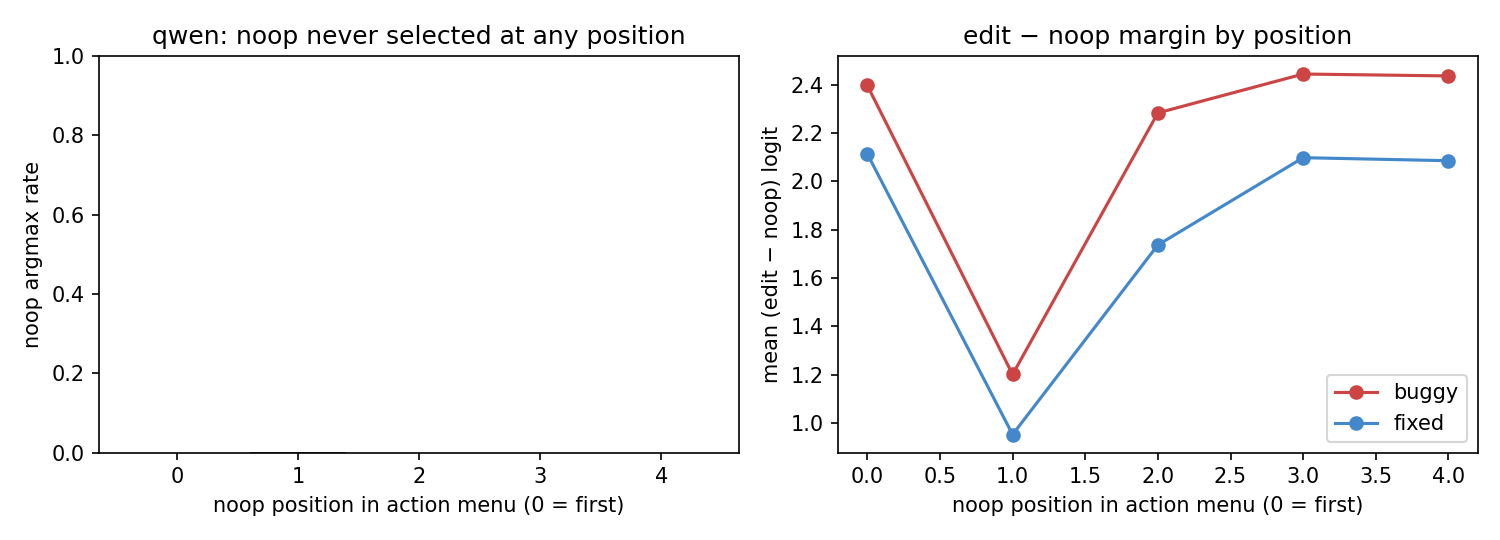
\includegraphics[width=0.92\linewidth,height=\textheight,keepaspectratio,alt={Action-menu controls (Qwen, 499 SWE-bench-Verified-derived code\_tests prompts). Left: noop argmax rate by its position in the action menu (0 = first); noop is selected in 1/4,990 prompts total, \ensuremath{\leq}0.1\% at every position. Right: mean edit \ensuremath{-} noop logit by noop position and condition, order modulates the margin but never makes noop competitive. Binary-menu and abstract-label controls (text) tell the same story.}]{figures/action_order_control_qwen.png}
\caption{\textbf{Action-menu controls (Qwen, 499
SWE-bench-Verified-derived \protect\texttt{code\_tests} prompts).}
\emph{Left:} \protect\texttt{noop} argmax rate by its position in the
action menu (0 = first); \protect\texttt{noop} is selected in 1/4,990
prompts total, \ensuremath{\leq}0.1\% at every position. \emph{Right:} mean
\protect\texttt{edit\ \ensuremath{-}\ noop} logit by \protect\texttt{noop} position
and condition, order modulates the margin but never makes
\protect\texttt{noop} competitive. Binary-menu and abstract-label
controls (text) tell the same story.}\label{fig:action_order}
\end{figure}

\subsection{Five-action logit decomposition: the direction moves a
submargin, not
abstention}\label{five-action-logit-decomposition-the-direction-moves-a-submargin-not-abstention}

We report the \texttt{edit\ \ensuremath{-}\ noop} submargin, but Qwen's argmax is
usually \texttt{grep} or \texttt{edit}. To see what moving along the
direction does to the \emph{full} action distribution, we decompose all
five action logits under rank-1 additive steering with \(v_{\rm raw}\)
(whose unit is \(u_{\rm tx}\); the \S{}4.2 dose-response vector) at L24/pos
\ensuremath{-}1 on the 49 toy \texttt{code\_tests} tasks (reusing the \S{}4.2 sweep;
scripts in App. J; Fig. \ref{fig:five_action}).

Steering with \(v_{\rm raw}\) (unit \(u_{\rm tx}\)) moves the
\texttt{edit\ \ensuremath{-}\ noop} margin smoothly and monotonically (buggy mean
5.49 \ensuremath{\rightarrow} 0.95 logits across \ensuremath{\alpha} \ensuremath{\in} {[}\ensuremath{-}3, 3{]}) and reallocates the argmax
\textbf{between \texttt{grep} and \texttt{edit}}, \texttt{grep} falls
from 98\% to 4\% (buggy) as \ensuremath{\alpha} increases while \texttt{edit} takes over.
But \texttt{noop} is \textbf{never} the argmax at any steering strength
(0\% across all \ensuremath{\alpha} and both conditions) and stays at logit rank 5 of 5
throughout (clean \texttt{noop} sits \textasciitilde2 logits below the
next action). So the direction modulates the edit-vs-abstain
\emph{submargin} and dislodges the default \texttt{grep} hedge toward
\texttt{edit}, but it does \textbf{not} induce abstention or overturn
the first-token action-token preference. Thus \texttt{edit\ \ensuremath{-}\ noop} is
a diagnostic submargin rather than a faithful two-action policy model.
This is the steering analogue of the \S{}5.4 SAE-ablation observation
(flips are \texttt{grep\ \ensuremath{\rightarrow}\ edit}, never toward \texttt{noop}), shown
directly on the causal direction. A \textbf{discrete-patching}
five-action check on the same 49 toy tasks at L24/pos \ensuremath{-}1 (paired
residual substitution, not steering) confirms that \texttt{noop} remains
noncompetitive: \texttt{noop} is the argmax in \textbf{0/49} prompts
under both F\ensuremath{\rightarrow}B and B\ensuremath{\rightarrow}F patches. Discrete argmax changes occur within the
\texttt{grep}/\texttt{edit} pair, F\ensuremath{\rightarrow}B flips 13 of 49 buggy tasks from
clean \texttt{edit} argmax to patched \texttt{grep}, and B\ensuremath{\rightarrow}F flips 12 of
49 fixed tasks from clean \texttt{grep} argmax to patched \texttt{edit}.
The direction of discrete \texttt{grep}/\texttt{edit} reallocations is
substrate-dependent (the \S{}4.1 SWE-derived peak-cell check moves them the
opposite way, tracking the substrates' opposite clean
\texttt{edit}-prevalence), so we do not interpret these transitions as a
stable full-action policy. The robust five-action observation is
submargin modulation with \texttt{noop} non-induction.

\textbf{Five-action decomposition sanity check (Qwen + DeepSeek
single-token).} Table \ref{tab:five-action-cross-model} reports discrete
five-action patching at each model's reported action-position cell on
the 49 toy \texttt{code\_tests} paired tasks: Qwen at the canonical-menu
L24 causal readout site, and DeepSeek rerendered with the single-token
vocabulary \texttt{\{view,\ find,\ test,\ edit,\ done\}} from \S{}5.5 at
its L22 reported cell (an exact single-token follow-up to the \S{}5.5
menu-order control, \emph{not} the canonical multi-token
\texttt{noop}-proxy result of \S{}4.3). This is a \emph{sanity check on
what the intervention does to the full action distribution}, not a
causal-localization estimate: across both models, under the current
five-action renderer, the discrete intervention changes the
\texttt{edit\ \ensuremath{-}\ abstain} submargin in the expected direction while
leaving abstention noncompetitive, the abstention action (\texttt{noop}
or \texttt{done}) stays the argmax in \textbf{0/98 clean} (49 buggy + 49
fixed), \textbf{0/49} under F\ensuremath{\rightarrow}B, and \textbf{0/49} under B\ensuremath{\rightarrow}F, with
per-task argmax changes confined to non-abstention actions. Because the
five-action decomposition uses a newer renderer, we treat it as a sanity
check rather than as a replacement for the \S{}4.1 causal-localization
numbers; these current-renderer shifts are not used to revise the
archived \S{}4.1/\S{}4.3 causal-localization estimates, and artifact and
reconciliation details are in App. J.

\begin{table}[t]
\caption{\textbf{Five-action decomposition sanity check at reported
action-position cells (current renderer).} $N = 49$ toy \texttt{code\_tests}
paired tasks. Shifts are paired-bootstrap mean $[95\%~\mathrm{CI}]$ of the
signed change toward closure of the buggy/fixed margin gap in the
$\ell_{\rm edit} - \ell_{\rm abstain}$ margin (F$\to$B:
$m^{\rm clean}_{\rm buggy} - m^{\rm patched}_{\rm buggy}$, positive $=$ pushed
toward fixed; B$\to$F: $m^{\rm patched}_{\rm fixed} - m^{\rm clean}_{\rm fixed}$,
positive $=$ pushed toward buggy). \textbf{abstain} $=$ \texttt{noop} for Qwen,
\texttt{done} for DeepSeek's single-token follow-up. These current-renderer
shifts are a sanity check and are not used to revise the \S{}4.1/\S{}4.3
causal-localization estimates (App. J). The CodeGemma row is omitted pending an
unresolved renderer-comparability check (text).}
\label{tab:five-action-cross-model}
\centering
\setlength{\tabcolsep}{4pt}
\resizebox{\linewidth}{!}{%
\begin{tabular}{llrrll}
\toprule
model / menu & cell & F$\to$B shift [95\% CI], \% pos.\ & B$\to$F shift [95\% CI], \% pos.\ & abstain argmax (clean 0/98; F$\to$B; B$\to$F) & main argmax transitions \\
\midrule
Qwen-1.5B, canonical \texttt{view/grep/test/edit/noop} & L24/pos $-1$ & $+0.625\,[+0.546,+0.704]$, 96\% & $+0.596\,[+0.520,+0.672]$, 96\% & $0/98$ / $0/49$ / $0/49$ & F$\to$B: 13 \texttt{edit}$\to$\texttt{grep}; B$\to$F: 12 \texttt{grep}$\to$\texttt{edit} \\
DeepSeek-1.3B, single-token \texttt{view/find/test/edit/done} (\S{}5.5 follow-up) & L22/pos $-1$ & $+0.694\,[+0.500,+0.898]$, 67\% & $+0.714\,[+0.520,+0.908]$, 69\% & $0/98$ / $0/49$ / $0/49$ & F$\to$B: 7 \texttt{edit}$\to$\texttt{view}; B$\to$F: 9 \texttt{view}$\to$\texttt{edit} \\
\bottomrule
\end{tabular}}
\end{table}

\textbf{CodeGemma five-action decomposition (omitted, renderer
comparability).} The CodeGemma discrete five-action run at its L26
reported cell is omitted from Table \ref{tab:five-action-cross-model}
because its current-renderer numeric margins are not comparable to the
archived \S{}4.3 cached artifact (a renderer-comparability issue, not a
challenge to the \S{}4.3 reported-cell result). Qualitative \texttt{noop}
non-induction is unchanged, \texttt{noop} argmax remains \textbf{0/49}
under clean and patched conditions, with the numerical audit deltas and
artifact paths in App. J.

\begin{figure}
\centering
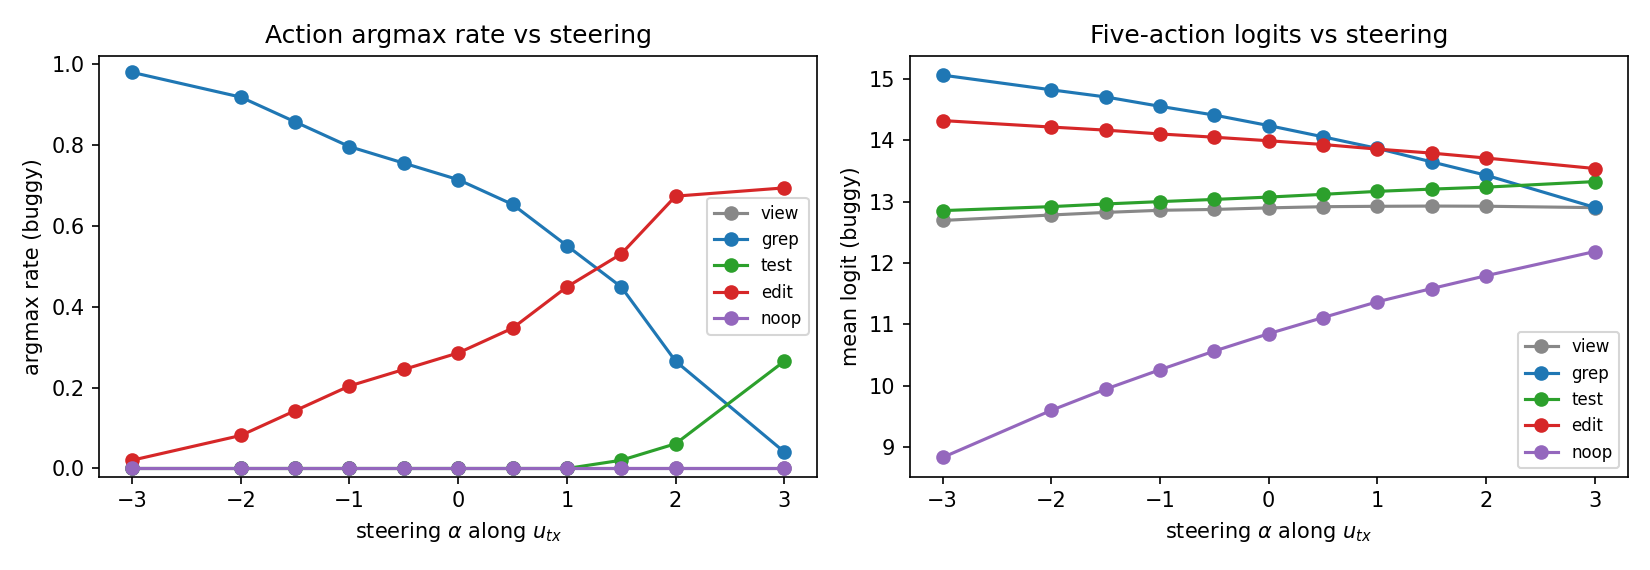
\includegraphics[width=0.92\linewidth,height=\textheight,keepaspectratio,alt={Five-action decomposition under steering along u\_\{\textbackslash rm tx\} (Qwen, L24/pos \ensuremath{-}1, 49 toy code\_tests tasks, buggy condition). Left: argmax rate per action vs steering \ensuremath{\alpha}, steering reallocates between grep and edit; noop stays at 0\% throughout. Right: mean logit per action vs \ensuremath{\alpha}, the edit \ensuremath{-} noop margin closes but noop remains lowest.}]{figures/five_action_decomp_qwen.png}
\caption{\textbf{Five-action decomposition under steering along
\(u_{\rm tx}\) (Qwen, L24/pos \ensuremath{-}1, 49 toy \protect\texttt{code\_tests}
tasks, buggy condition).} \emph{Left:} argmax rate per action vs
steering \ensuremath{\alpha}, steering reallocates between \protect\texttt{grep} and
\protect\texttt{edit}; \protect\texttt{noop} stays at 0\% throughout.
\emph{Right:} mean logit per action vs \ensuremath{\alpha}, the
\protect\texttt{edit\ \ensuremath{-}\ noop} margin closes but \protect\texttt{noop}
remains lowest.}\label{fig:five_action}
\end{figure}

\subsection{Transcript-robustness controls: the monitor is not
robust-superior to text
baselines}\label{transcript-robustness-controls-the-monitor-is-not-robust-superior-to-text-baselines}

A standing concern is that the synthesized pytest transcripts are clean
and regex-solvable. We apply four noisy/degraded transcript transforms
to the 499 Qwen \texttt{code\_tests} prompts and compare the residual
monitor (frozen \texttt{u\_tx}) against the App. G.8 regex classifiers
and a bag-of-words logistic baseline (5-fold CV). The monitor uses a
lean final-position projection that reproduces the headline AUC on clean
\texttt{code\_tests} (\textbf{0.989}), validating the scorer (scripts in
App. J).

{\def\LTcaptype{none} % do not increment counter
\begin{longtable}[]{@{}
  >{\raggedright\arraybackslash}p{(\linewidth - 8\tabcolsep) * \real{0.3750}}
  >{\raggedleft\arraybackslash}p{(\linewidth - 8\tabcolsep) * \real{0.1125}}
  >{\raggedleft\arraybackslash}p{(\linewidth - 8\tabcolsep) * \real{0.2250}}
  >{\raggedleft\arraybackslash}p{(\linewidth - 8\tabcolsep) * \real{0.2000}}
  >{\raggedleft\arraybackslash}p{(\linewidth - 8\tabcolsep) * \real{0.0875}}@{}}
\toprule\noalign{}
\begin{minipage}[b]{\linewidth}\raggedright
transcript
\end{minipage} & \begin{minipage}[b]{\linewidth}\raggedleft
monitor
\end{minipage} & \begin{minipage}[b]{\linewidth}\raggedleft
regex \texttt{contains}
\end{minipage} & \begin{minipage}[b]{\linewidth}\raggedleft
regex n-FAILED
\end{minipage} & \begin{minipage}[b]{\linewidth}\raggedleft
BoW
\end{minipage} \\
\midrule\noalign{}
\endhead
\bottomrule\noalign{}
\endlastfoot
clean (\texttt{code\_tests}) & 0.989 & 1.000 & 1.000 & 1.000 \\
+ unrelated failure (flaky) & 0.728 & \textbf{0.500} & 1.000 & 1.000 \\
+ many passing tests & 0.930 & 1.000 & 1.000 & 1.000 \\
truncated & 0.989 & 1.000 & 1.000 & 1.000 \\
summary line only & 0.896 & \textbf{0.500} & \textbf{0.500} & 1.000 \\
\end{longtable}
}

(The line-density regex tracks n-FAILED here; it too is 0.500 on
summary-only.) Two readings. (i) The brittle presence regex
\texttt{contains("FAILED")} breaks under a single appended unrelated
failure (0.50) and under summary-only transcripts (0.50, the pytest
summary says lowercase ``failed''), where the count/density regexes also
break. (ii) But the monitor is \textbf{not} robust-superior: it degrades
under distractors (flaky 0.73, many-passing 0.93, summary-only 0.90)
while a \textbf{bag-of-words baseline holds AUC 1.00 on every variant}.
In messy transcripts the monitor beats the literal-token regex but is
matched or beaten by bag-of-words throughout, consistent with the
monitor being an indirect transcript-evidence readout, not a superior
transcript classifier. A deployment-relevant test would need transcripts
where no surface text baseline suffices. Caveat: the bag-of-words
baseline is evaluated within each transform distribution by 5-fold CV;
it is a text baseline for the \emph{same} distribution, not a held-out
format-generalization result. A separate disjoint-vocabulary
held-out-template paraphrase test (App. G.17) reverses this comparison
for the literal and train-vocabulary keyword baselines on Qwen, where
the frozen Qwen residual direction also beats a train-fit BoW baseline
(0.943 vs 0.750 pooled AUC). That test is template-based, and its
held-out robustness is Qwen-specific: CodeGemma and DeepSeek reported
cells are negative, and it is not evidence of a semantic abstraction. It
therefore does not change the present finding that bag-of-words matches
or beats the monitor on these noisy/degraded pytest-style transcript
transforms. Artifacts and scripts are listed in App. J.

\subsection{Prior-gated, non-monotonic behavior across
scale}\label{prior-gated-non-monotonic-behavior-across-scale}

The 1.5B 0\%-abstention result (\S{}5.5) is not a scaling law. Reading the
first-token argmax over the 499 SWE \texttt{code\_tests} prompts at each
size, the do-nothing (\texttt{noop}) rate on passing (fixed) prompts is
\textbf{non-monotonic}: 0 / 11.0 / 0 / 0 / 5.0\% at 1.5B / 3B / 7B / 14B
/ 32B (95\% bootstrap CIs: 3B \([8.4,13.8]\), 32B \([3.2,7.0]\); 7B and
14B are exactly 0). It is nonzero exactly for the two sizes whose
dominant first-token hedge is \texttt{edit} (3B, 32B) and zero when the
hedge favors investigation (\texttt{view}/\texttt{grep}: 1.5B, 7B, 14B).
A position-balanced control at 7B confirms \texttt{noop} stays near 0\%
at every menu slot, so this is not a last-position artifact; the gate is
which action the prior favors.

\textbf{Removing the hedge unmasks abstention (binary menu).} A binary
\{edit, noop\} menu (1,996 prompts/size) raises the passing-prompt
\texttt{noop} rate for the view-prior \textbf{7B from 0\% to 11.9\%}
\([9.3,14.7]\) and for 3B from 11\% to 42.8\% \([39.2,46.4]\), while
1.5B stays low (1.4\%) and 14B/32B stay at 0\%. So the gate is the
graded \texttt{edit}-vs-\texttt{noop} margin, which removing the
investigation hedge overcomes only when that margin is already near zero
(7B, 3B), not for 14B/32B.

\textbf{Steering causally flips the action.} Rank-1 steering of the 3B
evidence direction (\(v_{\rm raw}\) at L32) on passing toys drives the
action from \texttt{edit} to \texttt{noop}: the \texttt{noop} argmax
rate rises 0\ensuremath{\rightarrow}51\% as \(\alpha\to+6\), and the \texttt{edit\ \ensuremath{-}\ noop}
margin crosses zero at \(\alpha\approx 4.0\). The signature that it
rides the \emph{evidence} axis, rather than a generic abstention push,
is that passing prompts flip \emph{before} failing prompts
(\(\alpha\approx+4\) vs \(+6\)). At the natural unit (\(\alpha=1\)) the
action does not flip, consistent with 1.5B; the direction is
\textbf{action-capable but suppressed at the operating point by the
prior}. Unlike the refusal direction \citep{arditi2024refusal}, which
controls behavior, this evidence direction flips the action only against
a permissive prior or under amplification.

\subsection{From static prompts to a live loop: over-editing and a
deployable
edit-veto}\label{from-static-prompts-to-a-live-loop-over-editing-and-a-deployable-edit-veto}

We move from the static single-turn decision to a minimal multi-turn
agent loop to ask whether the represented evidence predicts real
over-editing and whether the monitor is deployable as an edit-veto.
\textbf{Protocol} (faithful decisions, simulated execution): each turn
the model picks one action from \{view, grep, test, edit, noop\} given
the running history; \texttt{view} reveals the oracle code window,
\texttt{test} reveals the condition's pass/fail transcript,
\texttt{grep} is condition-neutral, and \texttt{edit}/\texttt{noop}
terminate. Observations are materialized from the paired data, so the
decisions are real model rollouts but no sandbox is executed. We run 40
SWE-derived tasks in both conditions on 1.5B/3B/7B/14B/32B from two
start states: \emph{from-issue} (issue + file list only, the agent must
act to gather evidence) and \emph{evidence-present} (code + transcript
in context). At each turn we record the monitor projection
(\(h\cdot u_{\rm tx}\) at the size's causal cell); the
\textbf{edit-veto} blocks an \texttt{edit} whose projection reads
``passing,'' using a \textbf{leave-one-out} threshold.

\textbf{Over-editing is real and severe, and evidence in context does
not stop it.}

{\def\LTcaptype{none} % do not increment counter
\begin{longtable}[]{@{}
  >{\raggedright\arraybackslash}p{(\linewidth - 8\tabcolsep) * \real{0.1579}}
  >{\raggedleft\arraybackslash}p{(\linewidth - 8\tabcolsep) * \real{0.2105}}
  >{\raggedleft\arraybackslash}p{(\linewidth - 8\tabcolsep) * \real{0.2105}}
  >{\raggedleft\arraybackslash}p{(\linewidth - 8\tabcolsep) * \real{0.2105}}
  >{\raggedleft\arraybackslash}p{(\linewidth - 8\tabcolsep) * \real{0.2105}}@{}}
\toprule\noalign{}
\begin{minipage}[b]{\linewidth}\raggedright
size
\end{minipage} & \begin{minipage}[b]{\linewidth}\raggedleft
over-edit (from-issue)
\end{minipage} & \begin{minipage}[b]{\linewidth}\raggedleft
over-edit (evidence)
\end{minipage} & \begin{minipage}[b]{\linewidth}\raggedleft
+ edit-veto (held-out)
\end{minipage} & \begin{minipage}[b]{\linewidth}\raggedleft
recall (evidence)
\end{minipage} \\
\midrule\noalign{}
\endhead
\bottomrule\noalign{}
\endlastfoot
1.5B & 35\% & 50\% & 22\% & 48\% \\
3B & 78\% & 88\% & \textbf{20\%} & 90\% \\
7B & 78\% & 98\% & \textbf{27\%} & 100\% \\
14B & 75\% & 100\% & 50\% & 100\% \\
32B & 75\% & 90\% & \textbf{18\%} & 100\% \\
\end{longtable}
}

For 3B--32B the agent edits already-passing code 75--100\% of the time,
and it does so \emph{more} with the passing transcript in context than
without (14B edits 100\% of passing tasks given the transcript). This is
the static ``evidence represented but not acted on'' finding manifesting
as real over-editing. 1.5B is the lone low point only because it is
\emph{indecisive} (it exhausts the turn budget investigating, not
abstaining) and its recall on buggy tasks is poor (48\%). A second
bottleneck is \textbf{evidence-gathering}: 3B runs \texttt{test} in only
2\% of from-issue loops (it edits blind), and for 7B testing
\emph{halves} over-editing (47\% when it tests vs 100\% when it does
not).

\textbf{The monitor is deployable as an edit-veto.} When the transcript
is in context, the internal pass/fail direction used as an edit-veto
with a held-out threshold cuts over-editing \textbf{2--5\ensuremath{\times} at every
scale} (88\ensuremath{\rightarrow}20\% at 3B; 98\ensuremath{\rightarrow}27\% at 7B; 100\ensuremath{\rightarrow}50\% at 14B; 90\ensuremath{\rightarrow}18\% at 32B),
preserving 60--94\% of correct edits (model-dependent; 3B cleanest at
94\% recall; decision-point AUC 0.68--0.89). The veto is useless without
gathered evidence (3B from-issue decision-point AUC 0.51, chance).

\textbf{A blunt prompt is brittle; the targeted veto is not.} An
explicit ``if the tests pass you MUST \texttt{noop}'' system instruction
cuts 3B over-editing to 15\% (recall 90\% preserved) but makes 7B
\texttt{noop} \emph{everything}, collapsing its recall to 8\%; it
over-applies the rule. The evidence-conditioned veto cuts over-editing
while \emph{preserving} recall, and in the realistic from-issue regime
the instruction is moot for models that do not gather the evidence (3B
tests 2\%). A targeted internal signal beats a blunt instruction.

\textbf{Caveats.} Pilot scale (N=40), simulated execution (synthesized
transcripts, no real test runs), greedy menu-constrained action
selection (not free-form generation), and held-out (not
cross-distribution) veto thresholds. The robust signals are the
\emph{severity} of over-editing and its \emph{multiplicative} reduction
under the veto; exact percentages will move with scale and protocol.

\section{Discussion and Limitations}\label{discussion-and-limitations}

\textbf{The mechanism is the constant; the behavior is the variable.}
Three results across the Qwen2.5-Coder ladder (\S{}4.4, \S{}5.8--5.9) recast
the static dissociation detailed below as one corner of a graded
picture. \emph{(i)} The causal pass/fail readout is \textbf{universal},
a late action-position site at every scale (1.5B--32B), following a
relative-depth law that drifts toward the final layer (width, not just
depth, pushes it deeper) and growing \textasciitilde18\ensuremath{\times} in causal
effect. \emph{(ii)} Whether that evidence changes the \textbf{action} is
\textbf{non-monotonic and prior-gated}: the do-nothing rate on passing
prompts is 0/11/0/0/5\% (1.5B\ensuremath{\rightarrow}32B), nonzero only when the first-token
prior is \texttt{edit}-dominant, and a binary menu or rank-1 steering
can override it; the evidence is action-capable but suppressed at the
operating point. \emph{(iii)} In a live loop the represented evidence
predicts \textbf{severe over-editing} (75--100\% of already-passing
tasks for 3B--32B; unreduced by having the transcript in context), which
the internal direction, used as a held-out \textbf{edit-veto}, cuts
2--5\ensuremath{\times} at high recall. The original 0\%-at-1.5B result is thus the
small-model, investigation-prior corner of this picture, and the monitor
(mechanistic, not a better transcript classifier) is nonetheless
\textbf{deployable} when read internally in the loop, where it beats a
blunt ``stop if passing'' instruction that destroys recall. The
remainder of this section details the static foundation these results
build on.

\textbf{A represented-evidence-vs-action dissociation in coding-agent
prompts.} Compute the classifier score \(s=-h\cdot u_{\rm tx}\) at
\texttt{resid\_pre{[}L\_site,\ pos\ \ensuremath{-}1{]}} (Qwen causal peak / each
other model's reported action-position cell) and threshold: this
one-dot-product projection separates matched failing-transcript/buggy
from matched passing-transcript/fixed prompts at AUC 0.989 / 0.950 /
0.888 (Qwen / CodeGemma / DeepSeek; 499 / 497 / 499 paired prompts). The
contradictory-transcript control (\S{}5.2; run on all three models in App.
G.16 with \(|\Delta\mathrm{Code}|/|\Delta\mathrm{Transcript}| < 0.02\)
everywhere) shows the direction tracks \textbf{transcript text}, not
code semantics. \textbf{In the clean synthesized-transcript setting we
evaluate, direct parsing is the right implementation}, App. G.8 reports
a \texttt{contains("FAILED")} regex at AUC 1.000, and App. G.10's
single-turn edit-veto simulation has the regex (100\% / 0\% blocked /
useful-edit loss) strictly dominating the projection (84.4--100\% /
11.9--29.2\% across three models). \textbf{Practical corollary: an
internal-state edit-veto is no better than reading the transcript here.}
The residual monitor is \textbf{not proposed as a better transcript
classifier}; its value is mechanistic, it identifies where explicit
pass/fail evidence is read out at the action-token decision and shows
this evidence causally moves the \texttt{edit\ \ensuremath{-}\ noop} margin without
dominating first-token argmax (\S{}4.1--\S{}4.2; \S{}4.1, Table
\ref{tab:swe-peak-patching} makes the decodability-vs-causal-use
separation explicit: L12/pos \ensuremath{-}1 is more decodable yet much smaller
causally). The direction sits within the representation-engineering
\citep{zou2023representation, rimsky2024caa} line of read-and-control
work, and 10 random toy pairs already reach AUC within 0.001 of the
full-49 baseline (App. G.4). The no-transcript Qwen variant is
\textbf{decisively negative}: at L24/pos \ensuremath{-}1 on the same 499 prompts,
none of the tested linear readouts discriminates buggy from fixed
(frozen \(u_{\rm tx}\) AUC 0.499; fresh contrastive direction LOO 0.521;
1536-D LR probe LOO 0.518; App. G.9); the mechanism is bound to the
transcript pathway for this L24-linear-monitor approach.

\textbf{Temporal separation within context.} The multi-turn control in
\S{}5.3 strengthens the mechanistic interpretation: the direction is not
only reading an adjacent pass/fail token, since moving the transcript
two turns upstream still leaves a 0.807 AUC signal at the final action
position. This result is Qwen-only and still within a single rendered
context; the transcript is positionally distant but not evicted. It also
beats only a stateless turn-local parser, not a full-history or stateful
parser that records test outcomes as they appear. We therefore treat it
as evidence of a carried-forward within-context representation, not
deployment superiority over text parsing.

\textbf{Bounded Qwen paraphrase generalization.} App. G.12 runs each
model's paraphrase paired-prompt set (499/498/499 for
Qwen/CodeGemma/DeepSeek, the shorter paraphrase prompts incur fewer
CodeGemma token-cap drops than \S{}5.1's 497) through one deterministic
3-sentence natural-language paraphrase that contains none of the regex's
pytest tokens. On \textbf{Qwen} the projection at the canonical (L24,
pos=\ensuremath{-}1) gives AUC \textbf{0.995}: the readout is not the literal
\texttt{FAILED} token, which collapses to chance on the paraphrase. This
bounds the readout above the literal pytest format but does \textbf{not}
establish a semantic pass/fail abstraction: the paraphrase is
deterministic and keyed on condition (buggy \ensuremath{\rightarrow} ``did not match'' /
``differed'' / ``does not satisfy''; fixed \ensuremath{\rightarrow} ``matched'' / ``aligned'' /
``satisfies''), so any keyword regex tuned to its vocabulary trivially
achieves AUC \ensuremath{\approx} 1.0. The right interpretation is: \emph{on Qwen, the
direction generalizes from pytest-format transcripts to one
paraphrase-format transcript}. A stricter \textbf{disjoint-vocabulary
held-out-template} follow-up on Qwen (App. G.17, no held-out fitting)
addresses the keyword-leak: with two train and two held-out templates
whose discriminative content vocabulary is disjoint, the frozen
\(u_{\rm tx}\) reaches pooled AUC \textbf{0.943} on held-out templates
while literal and train-vocabulary keyword baselines are exactly at
chance (a train-fit bag-of-words reaches pooled 0.750). This is still
\textbf{not} a semantic pass/fail abstraction: the templates are
hand-authored and deterministic, not adversarial or LLM-generated.

\textbf{Cross-model paraphrase status.} Replicating the
held-out-template test on CodeGemma and DeepSeek at their \S{}4.3 reported
cells (frozen directions, no post-hoc search; App. G.17) shows the
held-out robustness is \textbf{Qwen-specific}: CodeGemma's direction
degrades to held-out pooled AUC 0.649 and DeepSeek's collapses to 0.619,
both below the model-independent BoW (0.750). On the deterministic App.
G.12 paraphrase the two models likewise collapse at their \S{}4.3 reported
cells (AUC 0.275--0.545). A post-hoc layer \ensuremath{\times} position sweep (App.
G.13--G.14) identifies non-canonical cells with high paraphrase AUC,
CodeGemma at (L19, pos=\ensuremath{-}4) via the canonical toy contrast (pytest 0.976,
paraphrase-real 0.939), DeepSeek at (L16, pos=\ensuremath{-}5) only after switching
from a 49-pair toy contrast to a 499-pair SWE-derived pytest-format
contrast (paraphrase-real 0.925). We report these as exploratory: both
cells were selected on the evaluation formats and lack held-out
validation, and the DeepSeek result is no longer the same methodology as
the canonical toy contrast. They support the weak claim that a
cross-format-discriminative cell \emph{can be found under post-hoc cell
selection} on each model, not the stronger methodological claim that the
\S{}4.3 reported-cell contrast would have found it. A multi-step
transcript-observing agent harness on a FixedBench-style stale/no-edit
task suite using SWE-agent or OpenHands-style scaffolds and stronger
paraphrase baselines (keyword regex, BoW logistic regression,
disjoint-vocabulary paraphrase templates, LLM-generated held-out
paraphrases, adversarial paraphrases) remain future work.

\textbf{The mechanism on Qwen, corresponding late-layer sites
elsewhere.} On Qwen a single 1536-dim direction at (L24, pos \ensuremath{-}1)
reproduces the entire behavioral \texttt{edit\ \ensuremath{-}\ noop} gap as a
continuous dose-response, with bidirectional symmetry and a confirmed
negative control on the \texttt{code} (no-test-transcript) variant. The
same reported-cell paired-patching intervention applied to CodeGemma-7B
(L26/28) and DeepSeek-Coder-1.3B (L22/24) at relative depths in
{[}0.857, 0.929{]} gives action-position paired-patching effects at the
reported cells on each model (\S{}4.3, App. D): F\ensuremath{\rightarrow}B +1.14 / B\ensuremath{\rightarrow}F +1.18 for
CodeGemma (on a bimodal substrate; the \S{}4.2 steering plot uses the
20-task responsive subset for a cleaner dose-response, while the \S{}5.1
monitor headline uses the all-49 direction), F\ensuremath{\rightarrow}B +0.19 / B\ensuremath{\rightarrow}F +0.18 for
DeepSeek (where the toy buggy/fixed gap itself is only +0.20, so the
\emph{absolute} behavioral saliency is small even though the
reported-cell paired-patching effect is present). Across models, the
causal evidence is uneven: Qwen has the full bidirectional sampled grid
and the max-statistic permutation null; CodeGemma has an exploratory
one-way F\ensuremath{\rightarrow}B layer\ensuremath{\times}position heatmap (App. D) plus paired reported-cell
values; DeepSeek has paired reported-cell values only. We therefore
treat the cross-model result as evidence for corresponding late-layer
action-position effects, not a fully validated shared circuit. The fact
that CodeGemma's SAE behavioral specificity does not replicate Qwen's
(App. H.6) is consistent with the homology being looser than a strict
shared circuit.

\textbf{Toy-vs-SWE-derived saliency divergence on DeepSeek.}
DeepSeek-1.3B's toy buggy-fixed gap is +0.20 logits but the same frozen
\(u_{\rm tx}\) produces a +5.64-logit gap on the
SWE-bench-Verified-derived eval (monitor AUC 0.888), a 28\ensuremath{\times} saliency
divergence we surface but do not disambiguate. The methodological
implication is that toy substrate alone is not a reliable predictor of
cross-model monitor strength (\S{}6; App. G.4).

\subsection{Limitations}\label{limitations}

This section summarizes the main limitations and the boundary of the
claims. The strongest claims in this paper apply to \emph{static paired
prompts containing pass/fail test transcripts under a fixed five-action
vocabulary}; the bullets below mark the boundary between what the
evidence supports and what we treat as open.

\textbf{Characterized by controls in App. G / H:}

\begin{itemize}
\tightlist
\item
  \emph{Transcript-text driver.} The \S{}5.1 monitor follows transcript
  text, not code semantics (\S{}5.2); a regex baseline matches its
  discrimination at AUC 1.000 (App. G.8). The Qwen lexical-redaction
  control (App. G.6) refines this: literal pass/fail tokens carry
  \textasciitilde12 AUC points, broader transcript structure the rest.
  Under noisy/degraded transcripts (\S{}5.7) the monitor is not
  robust-superior either: it degrades under distractors while a
  bag-of-words baseline holds AUC 1.00 on every variant.
\item
  \emph{0\% noop rate is not a noop-token artifact.} In Qwen
  action-vocabulary swaps, \texttt{noop}\ensuremath{\rightarrow}\texttt{done} and
  \texttt{noop}\ensuremath{\rightarrow}\texttt{skip} both preserve 0.0\% abstention rate (App.
  G.7).
\item
  \emph{Action-menu position effects characterized.} Position-balanced
  and binary named-menu controls show near-zero abstention is
  position-robust on Qwen and CodeGemma; abstract-label controls reveal
  strong surface-form letter priors. DeepSeek differs: the canonical
  \texttt{noop} label is multi-token, and a single-token rerun with
  \texttt{\{view,\ find,\ test,\ edit,\ done\}} shows a first-position
  bias. Therefore position-robust abstention claims are limited to Qwen
  and CodeGemma, and all first-token action claims remain
  prompt-conditioned rather than live-agent claims.
\item
  \emph{In-sample operating-point thresholds.} For Qwen, held-out 50/50
  + leave-one-repo-out give precision 0.96--0.97 (vs 0.973 in-sample)
  and fixed-condition FPR 3.2--3.5\% (vs 2.6\%); App. G.5. DeepSeek's
  G.10 row uses a computed but not separately tabled held-out 50/50
  threshold; CodeGemma's G.10 row remains in-sample under the all-49
  direction. Formal CodeGemma / DeepSeek held-out calibration tables
  remain future work.
\item
  \emph{Single-turn edit-action veto characterized (not multi-turn).}
  The projection blocks 84.4--100\% of fixed-condition first-token edit
  actions at 11.9--29.2\% useful-edit loss across three models (under
  the thresholds reported in App. G.10). A multi-step harness with
  retry-after-veto remains open (see below).
\item
  \emph{Temporal-separation control is Qwen-only and single-pass.} App.
  G.15 uses a constructed multi-turn prompt rendered as one context, not
  a live agent loop with KV-cache continuation or context eviction. The
  residual beats a stateless turn-local regex but not a full-history or
  stateful parser; the transcript remains textually present in the
  context.
\item
  \emph{SAE behavioral specificity is Qwen-specific and seed-fragile
  (exploratory).} The precise +34\% margin reduction and 80\%
  argmax-flip numbers do not survive a seed=0 re-train; the qualitative
  small-k subset effect (\textasciitilde30\%) does (App. H.7).
\end{itemize}

\textbf{Scope limitations and open gaps:}

\begin{itemize}
\tightlist
\item
  \emph{\texttt{grep}/\texttt{view} may be investigation, not a failure
  to abstain.} The non-\texttt{noop} argmax is usually \texttt{grep} or
  \texttt{view}, which are evidence-gathering moves; first-token
  selection cannot separate ``investigating before deciding'' from
  ``declining to abstain.'' Distinguishing them requires a multi-step
  harness (future work item 1 below).
\item
  \emph{No code-only detection.} Without a transcript, the tested Qwen
  L24 linear monitor is near chance (App. G.9); it is a
  transcript-evidence readout, not a code-correctness detector.
\item
  \emph{Not the agent-loop SWE-bench.} Our evaluation is on SWE-bench-
  Verified-\emph{derived} static paired prompts (window + synthesized
  transcript), not the official agent benchmark
  \citep{jimenez2024swebench}.
\item
  \emph{Toy substrate scope.} 49 LLM-generated single-file Python toys;
  untested on multi-file patches, longer contexts, or non-Python.
\item
  \emph{Three chat-fine-tuned code models.} Untested on base models,
  mixture-of-experts (MoE), or non-code instruction-tuned models.
  Monitor strength varies (AUC 0.989/0.950/0.888); DeepSeek's
  toy-vs-SWE-derived saliency divergence (\S{}6) is unresolved.
\item
  \emph{Cross-model reported-cell follow-up is uneven.} \S{}4.3 / App. D
  reported-cell values on CodeGemma (L26) and DeepSeek (L22) are not
  full bidirectional grids; the \S{}4 CodeGemma steering plot uses a
  20-task responsive subset chosen post-hoc (the \S{}5.1 headline uses all
  49 toys).
\item
  \emph{In-context attribution is window-limited.} Cache covers only the
  last 32 token positions (App. I).
\item
  \emph{\texttt{edit\ \ensuremath{-}\ noop} is a submargin, not the full action
  decision.} Argmax rarely lands on \texttt{noop} regardless of
  projection. Qwen has steering-based and discrete-patching five-action
  decompositions (\S{}5.6, \S{}4.1); \S{}5.6 adds a DeepSeek single-token
  \texttt{done} reported-cell discrete check, and the CodeGemma
  reported-cell discrete check is flagged as an unresolved consistency
  check (see \S{}5.6 audit note). What remains open is full cross-model
  layer\ensuremath{\times}position five-action localization, cross-model steering
  decompositions, and an exact DeepSeek treatment of the canonical
  multi-token \texttt{noop} menu via sequence-level action scoring.
\end{itemize}

\textbf{Still open future experiments,} in priority order:

\begin{enumerate}
\def\labelenumi{\arabic{enumi}.}
\tightlist
\item
  \textbf{Real-execution agent-loop veto study.} \S{}5.9 reports a
  \emph{pilot} multi-turn loop with simulated observations (N=40, greedy
  menu-constrained actions) that already shows severe over-editing and a
  held-out edit-veto. What remains is a \emph{real-execution} harness on
  a FixedBench-style stale/no-edit suite
  \citep{fixedbench2025, yang2024sweagent} in which the agent runs
  actual tests, proposes free-form patches, and the veto includes
  retry-after-veto dynamics and per-model/per-repository threshold
  calibration at scale. The single most important follow-up.
\item
  \textbf{Full cross-model five-action \emph{patching} decompositions.}
  Qwen has both steering-based and discrete-patching five-action
  decompositions (\S{}5.6, \S{}4.1); \S{}5.6 adds a DeepSeek single-token
  \texttt{done} reported-cell discrete check (L22/pos \ensuremath{-}1) and reports a
  CodeGemma reported-cell discrete check (L26/pos \ensuremath{-}1) as an unresolved
  consistency check. What remains is \emph{full bidirectional grids} on
  CodeGemma and DeepSeek (currently only paired reported-cell values), a
  CodeGemma rerun under a unified prompt renderer that reconciles with
  the \S{}4.3 May-2026 artifact, and a DeepSeek decomposition using
  sequence-level action scoring for the canonical multi-token
  \texttt{noop} label, or a fully consistent single-token abstention
  vocabulary used throughout the DeepSeek analyses.
\item
  \textbf{Held-out transcript-format robustness.} A disjoint-vocabulary
  held-out-template paraphrase test is now done on Qwen (App. G.17):
  frozen \(u_{\rm tx}\) reaches AUC 0.943; literal and train-vocabulary
  keyword baselines are at chance; train-fit BoW reaches pooled AUC
  0.750. The cross-model reported-cell follow-up is also done and is
  \textbf{negative}: at their \S{}4.3 reported cells (frozen directions, no
  post-hoc search) CodeGemma degrades to held-out AUC 0.649 and DeepSeek
  collapses to 0.619, so the robustness is Qwen-specific. What remains
  is adversarial and LLM-generated held-out paraphrases and
  train-on-one-format/test-on-another generalization.
\item
  \textbf{Full cross-model causal localization.} CodeGemma and DeepSeek
  bidirectional grids and max-statistic permutation nulls (currently:
  CodeGemma has an exploratory one-way F\ensuremath{\rightarrow}B heatmap plus reported-cell
  paired values, App. D; DeepSeek is reported-cell paired only);
  DeepSeek should use a single-token abstention label
  (e.g.~\texttt{done}) for exact action-level margins.
\item
  \textbf{Held-out threshold calibration for CodeGemma and DeepSeek}
  (the Qwen 50/50 + leave-one-repo-out procedure of App. G.5).
\end{enumerate}

Beyond the \S{}5.9 pilot (simulated observations, N=40), a real-execution
agent-loop study would need to define gate semantics, retry-after-veto
behavior, and per-model/per-repository threshold calibration at scale,
with actual test runs and free-form patches rather than the simulated
observations and menu-constrained actions used here; Appendix G.10 is a
separate single-turn edit-action veto simulation.

\section{Conclusion}\label{conclusion}

Our central finding is a represented-evidence-vs-action gap that is
\emph{graded across scale}: a model carries pass/fail evidence
internally and it causally moves the edit-vs-abstain margin, but whether
it changes the action depends on the first-token action prior. Across
Qwen2.5-Coder 1.5B--32B the causal readout is universal (an
action-position residual direction at relative depth 0.86--0.96, the
effect growing \textasciitilde18\ensuremath{\times}), while the do-nothing rate on passing
prompts is non-monotonic (0/11/0/0/5\%) and gated by whether the prior
is edit-dominant; a binary \{edit, noop\} menu and rank-1 steering can
override the gate (\S{}4.4, \S{}5.8). Contradictory-transcript, no-transcript,
and text-baseline controls bound what the static monitor is: it tracks
transcript text, not code correctness, and a regex matches it when the
transcript is present, so its static value is mechanistic rather than as
a better classifier. In a live multi-turn loop, however, the represented
evidence predicts severe over-editing (3B--32B edit already-passing code
75--100\%, unreduced by having the transcript in context), and the same
internal direction, used as a held-out edit-veto, cuts over-editing
2--5\ensuremath{\times} at high recall and beats a blunt ``stop if passing'' instruction
that destroys recall (\S{}5.9). The mechanism is the constant and the
behavior is the variable; the main open question is whether these gains
survive a real-execution agent loop at scale (\S{}6.1).

\section{Ethics and Data Use}\label{ethics-and-data-use}

The 499 SWE-bench Verified instances we evaluate (App. G.1) derive from
public GitHub repositories under their respective open-source licenses
(\texttt{django} BSD, \texttt{sympy} BSD, \texttt{sphinx} BSD,
\texttt{matplotlib} PSF-like, \texttt{scikit-learn} BSD,
\texttt{pylint-dev} GPL-2.0, \texttt{requests} Apache 2.0,
\texttt{pytest-dev} MIT, \texttt{pydata} BSD, \texttt{astropy} BSD). The
Verified subset is redistributed under SWE-bench's terms
\citep{jimenez2024swebench}; we re-use 499 of its 500 instances (1
dropped at ingestion: file 404 at the base commit). We do not
redistribute full upstream source files or full oracle code windows. The
activation-cache release consists primarily of residual activations,
projection scores, run manifests, and limited prompt-derived metadata;
as documented in App. J.5, this metadata can include last-token text or
token ids that may contain short fragments of the oracle code window.

The 49-task toy substrate (App. B.1) was generated by
\texttt{anthropic/claude-sonnet-4.5} (OpenRouter alias / likely snapshot
probe and prompt template in App. B.1.1; cf.
\texttt{scripts/generate\_tasks.py}) and validated by executing
\texttt{pytest} in a sandbox: only \texttt{(buggy,\ fixed)} pairs where
\texttt{pytest} exits 1 on \texttt{buggy} and 0 on \texttt{fixed} were
accepted (49 of 77 generated pairs; rejection log in
\texttt{data/\_generation\_log.jsonl}). Because this substrate is
machine-generated research data, we disclose its provenance and
validation procedure explicitly; we acknowledge it may inherit biases of
the generator's data distribution (e.g.~coverage skew toward common
Python idioms, possible duplication of GitHub-derived patterns). The
substrate is released under the same license as the rest of the
repository.

\section{LLM Use Disclosure}\label{llm-use-disclosure}

The 49-task toy substrate was generated by
\texttt{anthropic/claude-sonnet-4.5} as described in App. B.1.1 and
validated by executing \texttt{pytest}. LLM coding-agent assistance was
also used to draft or modify analysis and paper-editing code, and for
editorial feedback, revision planning, and prose copy-editing; all
scripts were executed under author control, and all reported metrics
come from cached model outputs and analysis artifacts. LLMs were not
used to generate model logits or experimental measurements directly. All
reported numbers come from the scripts, cached activations, and model
outputs described in App. J. The deterministic G.12 paraphrase strings
and the G.17 train/held-out paraphrase templates were hand-authored.

\section{Broader Impacts}\label{broader-impacts}

This paper's \emph{mechanistic} finding is a residual-stream direction
at the action position that tracks pass/fail-test-transcript evidence
and causally modulates the \texttt{edit\ \ensuremath{-}\ noop} margin. App. G.9 rules
out a no-transcript deployment for \textbf{this Qwen L24/pos \ensuremath{-}1 linear
monitor specifically}; it does \textbf{not} rule out other layers,
nonlinear probes, full agent traces, or semantic-code-analysis methods
on the no-transcript distribution. App. G.10 sketches a hypothetical
edit-action veto: at the action-token decision point of an agent that
has been shown a transcript, the projection wired as an
\texttt{edit}-veto blocks 84.4--100\% of fixed-condition first-token
edit actions at 11.9--29.2\% useful-edit loss across three models (under
the thresholds reported in App. G.10, Qwen and DeepSeek held-out 50/50;
CodeGemma in-sample balanced-accuracy on the all-49 direction). We do
\textbf{not} claim this is a deployment-ready gate; in the clean pytest
setting the regex gate strictly dominates (App. G.10), and we do not
validate it in a multi-step agent harness; that remains future work
(\S{}6.1).

The cost asymmetry between gate errors is deployment-specific. In
\textbf{interactive repair settings}, false-noops may be especially
costly because a real fix is silently suppressed by the gate and the
human reviewer never sees it; useful-edit loss is the relevant column.
In \textbf{high-volume stale-issue triage or repository-cleanup
settings} where most candidate tasks are already resolved, spurious-edit
reduction may dominate because every unnecessary edit becomes review
burden. We do not model either cost regime end-to-end. In our
single-turn setting the regex gate strictly dominates the projection on
both metrics (App. G.10), so the cost-asymmetry calculus only becomes
interesting in settings where the trivial pytest-token regex gate is
unavailable or insufficient (held-out or adversarial paraphrases,
genuinely ambiguous transcripts, or temporally-separated multi-turn
traces when the comparison is restricted to stateless turn-local
parsing).

\textbf{Why use a residual monitor at all?} On each model's
paired-prompt set (499/497/499 for Qwen/CodeGemma/DeepSeek) the regex
baseline beats the projection both as a classifier (App. G.8: AUC 1.000
vs 0.989) \textbf{and} as an edit-action gate (App. G.10: 100\% / 0\% vs
84.4--100\% / 11.9--29.2\%). In the clean synthesized-transcript setting
we evaluate, direct parsing is the right implementation. One regime
where the residual beats a \textbf{stateless turn-local} regex is
\textbf{temporal separation} (Qwen; App. G.15): with the transcript
moved two agent turns upstream, the projection still discriminates at
AUC 0.807 while a turn-local regex, parsing only the current
observation, reads chance, because the decision-point context holds no
pass/fail token. A full-history regex or a stateful parser that records
earlier test outcomes would still recover it, so this is mechanistic
evidence that the model carries the upstream transcript verdict to the
action position, \textbf{not} deployment superiority over text parsing.
The remaining settings where a residual monitor might be interesting are
not the clean or deterministic formats tested here, but harder settings
where surface text baselines are deliberately held out or fail:
adversarial paraphrases, LLM-generated held-out paraphrases, genuinely
ambiguous transcripts, or live multi-step traces where the relevant
evidence is no longer turn-local. We test two Qwen paraphrase settings:
a deterministic paraphrase where keyword/BoW baselines also match the
monitor (App. G.12), and a disjoint-vocabulary held-out-template test
where Qwen reaches AUC 0.943 while literal and train-vocabulary keyword
baselines are at chance and train-fit BoW reaches pooled AUC 0.750 (App.
G.17). Cross-model reported-cell follow-up of the latter is negative
(CodeGemma 0.649, DeepSeek 0.619), so this robustness is Qwen-specific.
Neither paraphrase setting is validated as a gate, and neither
establishes a semantic abstraction. The code-only absent-transcript
setting is negative for this Qwen L24 linear monitor (App. G.9). The
mechanistic finding, identifying \emph{where} explicit pass/fail
evidence is read out at an action-token residual-stream site and showing
it causally affects the \texttt{edit\ \ensuremath{-}\ noop} submargin, and that the
direction \textbf{propagates the transcript verdict across intervening
turns} (App. G.15), does not depend on the projection being a
deployment-superior gate.

The same mechanism is \textbf{bidirectionally steerable} on Qwen (\S{}4.2):
an adversary with model access could add \(-\alpha\,v_{\rm raw}\) at the
(L24, pos \ensuremath{-}1) cell to push the model toward \texttt{edit}, amplifying
over-editing, the opposite of the intended deployment use. Detecting
such tampering would require monitoring the projection itself, not only
the emitted action.

Generalization caveats compound this. Monitor strength varies materially
across model families: AUC ranges from 0.888 (DeepSeek) to 0.989 (Qwen),
and in-sample fixed-condition FPR ranges from 2.6\% (Qwen) to 19.6\%
(DeepSeek). CodeGemma's fixed-condition FPR also varies by repository:
\texttt{django/django} is 13.0\%, \texttt{sphinx-doc/sphinx} is 22.7\%,
and the small \texttt{pylint-dev/pylint} slice is 40.0\% on only 10
pairs (App. G.3). Any future deployment study would need per-model
\textbf{and} per-(model, repository) calibration; these integration
considerations are paper-internal, not a deployment recipe. \textbf{We
have not validated this monitor end-to-end in a real agent loop}, and
discourage deployments that skip that validation step.

\section{References}\label{references}

\bibliography{refs}

\appendix

\section*{Appendix Contents}\label{appendix-contents}
\addcontentsline{toc}{section}{Appendix Contents}

\textbf{Contents.} Appendix A: extended related work. B: detailed
methods. C: behavioral \ensuremath{\Delta}-margin and probe saturation. D: Qwen patching
heatmap, exploratory CodeGemma heatmap, and Qwen negative control. E:
per-task steering dose-response curves. F: stale-variant failure
analysis and toy-monitor LOOCV. G: full SWE-derived evaluation including
specificity baselines, per-repo CodeGemma regression analysis, and
per-repo calibration counterfactual; G also contains the
temporal-separation control (G.15), the cross-model
contradictory-transcript control (G.16), and disjoint-vocabulary
held-out paraphrase robustness (G.17): Qwen positive, CodeGemma/DeepSeek
negative at their reported cells. H: full SAE decomposition (Qwen and
CodeGemma). I: in-context attribution within the cached last-32-token
window. J: reproduction recipe and artifacts.

\textbf{Appendix evidence map.}

{\def\LTcaptype{none} % do not increment counter
\begin{longtable}[]{@{}
  >{\raggedright\arraybackslash}p{(\linewidth - 4\tabcolsep) * \real{0.3704}}
  >{\raggedright\arraybackslash}p{(\linewidth - 4\tabcolsep) * \real{0.3333}}
  >{\raggedright\arraybackslash}p{(\linewidth - 4\tabcolsep) * \real{0.2963}}@{}}
\toprule\noalign{}
\begin{minipage}[b]{\linewidth}\raggedright
Evidence location
\end{minipage} & \begin{minipage}[b]{\linewidth}\raggedright
Purpose
\end{minipage} & \begin{minipage}[b]{\linewidth}\raggedright
Status
\end{minipage} \\
\midrule\noalign{}
\endhead
\bottomrule\noalign{}
\endlastfoot
B--E & Qwen causal localization: toy substrate, hooks, patching,
steering & full bidirectional sampled grid + max-statistic permutation
null on Qwen; CodeGemma has an exploratory one-way F\ensuremath{\rightarrow}B heatmap (App. D)
plus reported-cell paired values; DeepSeek is reported-cell paired
only \\
\S{}4.1 SWE-derived peak-cell check & Qwen peak-cell paired patching on
N=200 SWE-derived \texttt{code\_tests} paired prompts at L24/pos \ensuremath{-}1 with
L12/pos \ensuremath{-}1 and L24/pos \ensuremath{-}8 controls; all five action logits & supports
transfer of the causal readout (F\ensuremath{\rightarrow}B +0.314, B\ensuremath{\rightarrow}F +0.311 at causal cell;
\textasciitilde10\ensuremath{\times} smaller at L12, \textasciitilde0 at pos \ensuremath{-}8;
\texttt{noop} never argmax), not a full SWE-derived localization grid \\
\S{}4.3 + \S{}\ref{sec:tok-audit} & DeepSeek action-margin / patching analyses
& first-subword proxy under canonical menu (\texttt{noop} multi-token);
single-token \texttt{done} rerun in \S{}5.5 covers menu-order control; \S{}5.6
adds a single-token discrete patching follow-up at L22/pos \ensuremath{-}1 for the
five-action decomposition \\
G.1--G.2 & SWE-derived ingestion and monitor baselines & supports
monitor evaluation \\
G.8--G.10 & regex, no-transcript, single-turn gate controls & critical
scope controls \\
G.12 & deterministic paraphrase control + keyword/BoW text baselines
(run) & text baselines reach AUC 1.0; not a semantic proof \\
G.13--G.14 & cross-format post-hoc sweeps & exploratory,
selection-biased \\
G.15 & temporal-separation control & Qwen-only mechanistic control \\
G.16 & cross-model contradictory-transcript control & critical
transcript-vs-code control \\
G.17 & Disjoint-vocabulary held-out paraphrase robustness & Qwen frozen
\(u_{\rm tx}\) reaches AUC 0.943; CodeGemma and DeepSeek reported-cell
directions degrade to 0.649/0.619; literal and train-vocabulary keyword
baselines are at chance; train-fit BoW pooled AUC 0.750; template-based,
not semantic abstraction \\
\S{}5.5 & action-menu / position-balance controls (Qwen, CodeGemma,
DeepSeek single-token rerun) & abstention position-robust on
Qwen/CodeGemma; DeepSeek first-position bias \\
\S{}5.6 & five-action steering + Qwen discrete-patching decomposition;
DeepSeek single-token \texttt{done} reported-cell discrete check
(L22/pos \ensuremath{-}1); CodeGemma reported-cell discrete check (L26/pos \ensuremath{-}1)
flagged as unresolved consistency check vs.~\S{}4.3 (audit JSON) & Qwen and
DeepSeek single-token follow-up move the \texttt{edit\ \ensuremath{-}\ abstain}
submargin while abstention stays argmax 0/49 under all clean and patched
conditions; CodeGemma submargin magnitudes not directly comparable to
\S{}4.3 pending rerun \\
\S{}5.7 & noisy-transcript controls (monitor vs regex vs BoW) & text
baselines match/beat the monitor \\
Methods / App. B tokenization audit & exact-context action tokenization
& Qwen/CodeGemma single-token; DeepSeek \texttt{grep}/\texttt{noop}
multi-token \\
H & SAE decomposition (figure in appendix) & exploratory,
seed-fragile \\
I & in-context attribution & exploratory \\
J & reproduction and artifacts & reproducibility \\
\end{longtable}
}

\section{Extended Related Work}\label{extended-related-work}

The \S{}2 references compressed several lines of evidence per cited paper.
The per-paper detail:

\textbf{Coding-agent action bias on stale tasks: TEBench and
FixedBench.} TEBench \citep{shang2026tebench} is a project-level
\emph{test-evolution} benchmark that catalogs three subproblems,
Test-Breaking (tests that need modification because production code
changed), Test-Stale (tests that pass but no longer meaningfully
validate updated behavior), and Test-Missing, and asks coding agents to
identify and update tests. The Test-Stale subset is the piece closest to
a ``no-code-change'' task, but the benchmark's framing is \emph{test}
evolution, not no-code-change abstention. FixedBench
\citep{fixedbench2025}, from the SRI Lab at ETH Zürich, is the more
directly relevant behavioral benchmark for this paper's phenomenon: it
studies \emph{stale bug reports} where no code change is required and
reports undesirable code changes in 35--65\% of cases, depending on
model/harness. Our paired-task substrate is methodologically downstream
of both; we treat the over-editing phenomenon as the behavioral
substrate to mechanistically localize, but we evaluate the projection
monitor only on SWE-bench-Verified-derived static paired prompts that
contain explicit pass/fail transcripts. FixedBench is the behavioral
phenomenon a future no-transcript no-edit detector would target; App.
G.9 is \textbf{negative} for the specific Qwen L24 linear monitor
studied here (the tested linear readouts are near chance without a
transcript), so we do not claim a FixedBench-style no-transcript
detector (a gap we flag in \S{}6.1). The SWE-agent scaffold
\citep{yang2024sweagent} and Agentless decomposition
\citep{xia2024agentless} are the dominant agent architectures evaluated
on SWE-bench; an agent-loop veto monitor would sit at their
localization-vs-validation seam.

\textbf{Refusal-as-a-single-direction.} \citet{arditi2024refusal}
identify a single residual-stream direction that mediates refusal in
instruction-tuned chat models; ablating it suppresses refusal, adding it
induces refusal. Our contrast direction is structurally similar (one
direction, contrastive mean-of-fixed minus mean-of-buggy): the
unit-normalized direction \(u_{\rm tx}\) is used as a read-out axis for
monitoring, while the raw mean-difference vector \(v_{\rm raw}\) is used
for additive steering of the \texttt{edit\ \ensuremath{-}\ noop} margin in \S{}4.2. But
the \emph{quantity it controls} is narrower: it modulates a 2-action
submargin under code-plus-transcript prompts and tracks
pass/fail-transcript evidence (\S{}5.2), not a separately-encoded
abstention belief analogous to refusal. The methodological parent of the
steering direction itself, mean-difference of paired prompt activations,
is contrastive activation addition \citep{rimsky2024caa}; we cite the
older \emph{Activation Addition} \citep{turner2023actadd} for context,
but the specific paired-mean recipe used here is CAA.

\textbf{Activation steering for behavioral control.}
\citet{turner2023actadd} introduced \emph{Activation Addition} (ActAdd),
demonstrating that a single additive direction in residual space,
computed from contrastive prompt pairs, can steer model behavior without
optimization or labeled data. \citet{rimsky2024caa} formalize the
\emph{paired} mean-of-pairs variant (CAA) we actually use. Most directly
related, \emph{Manifold Steering} \citep{huang2025manifold} shows that
overthinking in large reasoning models can be captured by a
low-dimensional manifold and steered by intervening along the dominant
direction. The umbrella \emph{Representation Engineering}
\citep{zou2023representation} line frames the broader read/control
pipeline. Our monitor direction \(u_{\rm tx}\) is the same kind of
object (mean-difference at a fixed (layer, position) cell), but
identified by causal localization on edit-vs-noop rather than chosen a
priori for overthinking behavior.

\textbf{Activation patching for causal localization.} Activation
patching \citep{meng2022rome, wang2023ioi}, and circuit-level analysis
in general \citep{elhage2021mathematical}, are the standard tools for
identifying which residual stream sites carry information that a
downstream computation reads from. \citet{heimersheim2024patching} and
\citet{zhang2024patchingbestpractices} give practical guides and metric
recommendations (notably the logit-difference metric we adopt). Our use
of paired buggy/fixed prompts and the \texttt{edit\ \ensuremath{-}\ noop} margin
follows this protocol.

\textbf{Probes need control tasks.} \citet{hewitt2019probes} showed that
a high-AUC linear probe does not establish that the underlying model
\emph{uses} the probed feature, high probe accuracy can reflect probe
capacity rather than feature usage. Our probe results saturate at AUC \ensuremath{\approx}
1.0 across all layers; we treat them as necessary but not sufficient,
and rely on patching and steering for causal claims.

\textbf{Sparse features for code correctness.}
\citet{tahimic2025codecorrectness} train sparse autoencoders on code-LLM
residuals and identify directions correlating with code correctness,
finding test-case attention is the primary signal (echoing our finding
that \emph{test transcripts} are the sole behavioral driver). They study
correct-vs-incorrect \emph{code features}; we study the \emph{agent's
decision} to mutate the repository, which is upstream of and distinct
from correctness assessment, and we localize to a single (layer,
position) cell rather than a feature collection.

\section{Detailed Methods}\label{detailed-methods}

\subsection{Paired-task substrate}\label{paired-task-substrate}

Each task \texttt{t} provides two task snapshots with identical issue
text: \texttt{buggy/parser.py} where \texttt{pytest} reports a failure,
and \texttt{fixed/parser.py} where it passes. We generated 49 such pairs
across 12 archetypes via \texttt{anthropic/claude-sonnet-4.5} and
validated each by executing pytest in a sandbox: only pairs where
\texttt{fixed} exits 0 and \texttt{buggy} exits 1 are accepted. We
further evaluate five evidence variants per task:

\begin{itemize}
\tightlist
\item
  \texttt{issue\_only}: bug report only.
\item
  \texttt{code}: bug report + the buggy or fixed source.
\item
  \texttt{code\_tests}: + the corresponding pytest transcript.
\item
  \texttt{stale\_misleading}: bug report claims a bug, but the fixed
  code and passing transcript are shown (one-sided control).
\item
  \texttt{stale\_flaky}: as \texttt{stale\_misleading} but with one
  synthetic unrelated flaky failure spliced in
  (e.g.~\texttt{test\_network\_timeout} failing with a
  \texttt{ConnectionError}).
\end{itemize}

\begin{figure}
\centering
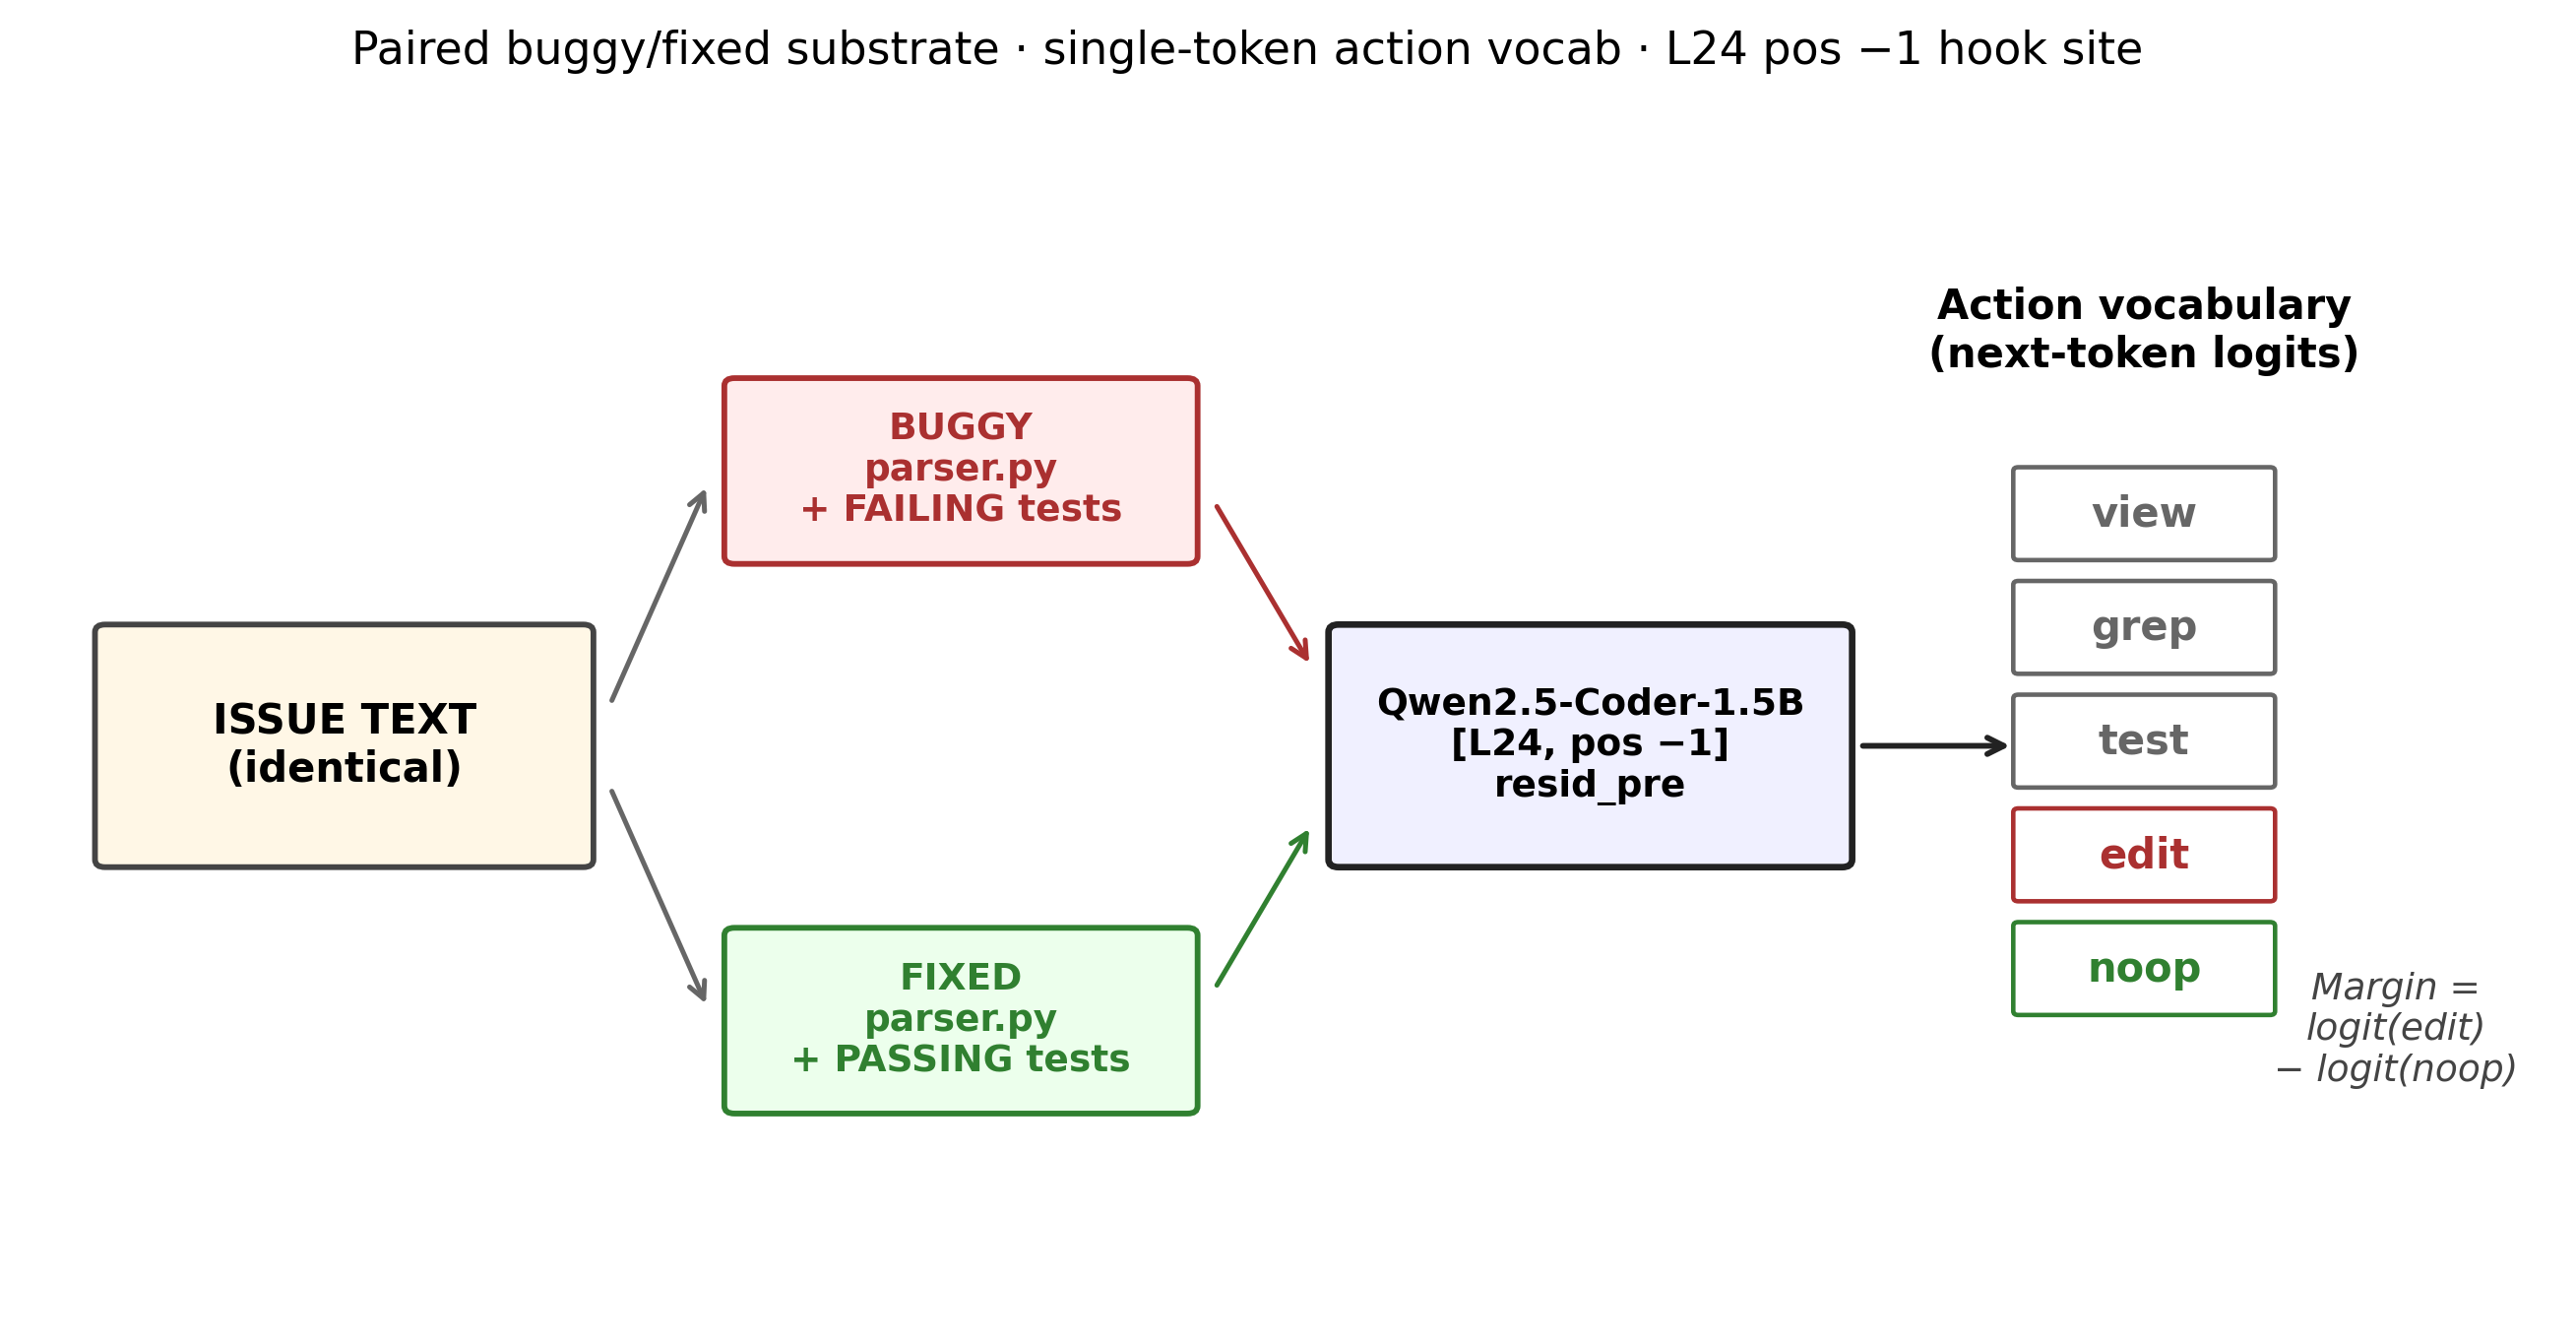
\includegraphics[width=0.9\linewidth,height=\textheight,keepaspectratio,alt={Paired buggy/fixed substrate and intervention site.}]{figures/paired_task_diagram.png}
\caption{Paired buggy/fixed substrate and intervention site.}
\end{figure}

\subsubsection{Toy task generation
procedure}\label{toy-task-generation-procedure}

\textbf{Generator model.} All 49 toy pairs were synthesized by
\texttt{anthropic/claude-sonnet-4.5} (OpenRouter alias; cf.
\texttt{src/no\_op\_circuit/llm.py} \texttt{DEFAULT\_MODEL}). The
OpenRouter alias resolves at call time to whatever Anthropic snapshot is
currently routed. The original generation run (2026-05-15) did not log
the provider's resolved \texttt{response.model} field, so the historical
snapshot used for the 49-task substrate is \textbf{irrecoverable} from
the existing \texttt{data/\_generation\_log.jsonl}. A re-probe of the
alias on 2026-05-17 routed to
\textbf{\texttt{anthropic/claude-4.5-sonnet-20250929}} (probe record at
\texttt{data/\_generation\_snapshot\_probe.json}); we treat this as the
most likely historical resolution but cannot confirm it. The
\texttt{llm.chat()} wrapper is patched to expose
\texttt{resolved\_model} on \texttt{ChatResult}, and
\texttt{scripts/generate\_tasks.py} writes it into
\texttt{\_generation\_log.jsonl}'s \texttt{resolved\_model} field, so
any future regeneration cannot lose this attribution.

\textbf{Sampling config.} Temperature \texttt{0.85},
\texttt{max\_tokens=4096}, OpenAI
\texttt{response\_format=\{"type":\ "json\_object"\}} for structured
output, no \texttt{top\_p} override (provider default). Three retries
with 4-second exponential backoff on \texttt{RateLimitError} /
\texttt{APIConnectionError}. Driver: \texttt{scripts/generate\_tasks.py}
invoking \texttt{no\_op\_circuit.dataset.generator.generate\_candidate}.

\textbf{Generation prompt.} The system message frames the task as
``propose a small Python paired (buggy, fixed) task for archetype
\emph{X}''; the user message attaches one hand-curated few-shot example
(\texttt{parser\_empty\_input}) plus the target archetype's
\texttt{description}, \texttt{example\_signature}, and \texttt{domains}
(from \texttt{data/archetypes.yaml}). The expected JSON schema specifies
\texttt{task\_id}, \texttt{issue\_text}, \texttt{primary\_file},
\texttt{test\_command}, \texttt{buggy\_files}, \texttt{fixed\_files},
and a single \texttt{test\_file}, full schema in
\texttt{src/no\_op\_circuit/dataset/schema.py}.

\textbf{Acceptance gate.} Each candidate is materialized to a temp
directory and run twice: once against \texttt{buggy/} and once against
\texttt{fixed/}. Acceptance requires \texttt{pytest} exit code 1 on
\texttt{buggy/} \textbf{and} exit code 0 on \texttt{fixed/}. Additional
gates: stdlib-only imports (rejects external dependencies), no use of
network fixtures, and a single-file primary-file requirement. Rejections
are logged with reason at \texttt{data/\_generation\_log.jsonl}.

\textbf{Yield.} 77 attempts \ensuremath{\rightarrow} 55 generation-stage accepts \ensuremath{\rightarrow} 49 final
pairs after the additional file-level / validation gates
(\textasciitilde37\% total rejection rate). Per-archetype
generation-attempt counts:

{\def\LTcaptype{none} % do not increment counter
\begin{longtable}[]{@{}lrr@{}}
\toprule\noalign{}
archetype & attempts & accepted (gen) \\
\midrule\noalign{}
\endhead
\bottomrule\noalign{}
\endlastfoot
off\_by\_one\_loop & 14 & 10 \\
off\_by\_one\_slice & 8 & 6 \\
missing\_empty\_case & 7 & 6 \\
missing\_return & 4 & 4 \\
mutable\_default\_argument & 4 & 4 \\
case\_sensitivity & 4 & 4 \\
wrong\_arithmetic & 8 & 5 \\
wrong\_comparison & 8 & 2 \\
wrong\_default\_arg & 4 & 3 \\
wrong\_sort\_order & 4 & 4 \\
swapped\_args & 4 & 3 \\
shallow\_copy\_bug & 8 & 4 \\
\textbf{total} & \textbf{77} & \textbf{55} (49 final) \\
\end{longtable}
}

The 49 final accepted tasks ship under \texttt{data/tasks/}; the full
rejection log is at \texttt{data/\_generation\_log.jsonl}.

\subsection{Action vocabulary}\label{action-vocabulary}

The prompt ends with
\texttt{\textless{}chat-template-end\textgreater{}\textbackslash{}nAction:}
and the model's first predicted token is read out. We restrict the
comparison to five named actions, \texttt{view}, \texttt{grep},
\texttt{test}, \texttt{edit}, \texttt{noop}. The scalar of interest is
the \texttt{edit\ \ensuremath{-}\ noop} logit margin (single-tokenness audited
below).

\subsection{Action-tokenization audit}\label{sec:tok-audit}

We verify single-tokenness in the \textbf{exact scored context}, the
first token after the final \texttt{Action:}, resolved by diffing
\texttt{encode(prefix)} against \texttt{encode(prefix+name)}, the same
rule the action-logit readout uses
(\texttt{scripts/check\_action\_tokenization.py};
\texttt{results/tokenization/}). The five names are single-token under
Qwen and CodeGemma, but \texttt{grep} and \texttt{noop} are \textbf{two
tokens} under DeepSeek:

{\def\LTcaptype{none} % do not increment counter
\begin{longtable}[]{@{}
  >{\raggedright\arraybackslash}p{(\linewidth - 10\tabcolsep) * \real{0.1667}}
  >{\raggedright\arraybackslash}p{(\linewidth - 10\tabcolsep) * \real{0.1667}}
  >{\raggedright\arraybackslash}p{(\linewidth - 10\tabcolsep) * \real{0.1667}}
  >{\raggedright\arraybackslash}p{(\linewidth - 10\tabcolsep) * \real{0.1667}}
  >{\raggedright\arraybackslash}p{(\linewidth - 10\tabcolsep) * \real{0.1667}}
  >{\raggedright\arraybackslash}p{(\linewidth - 10\tabcolsep) * \real{0.1667}}@{}}
\toprule\noalign{}
\begin{minipage}[b]{\linewidth}\raggedright
model
\end{minipage} & \begin{minipage}[b]{\linewidth}\raggedright
action
\end{minipage} & \begin{minipage}[b]{\linewidth}\raggedright
scored form
\end{minipage} & \begin{minipage}[b]{\linewidth}\raggedright
token ids
\end{minipage} & \begin{minipage}[b]{\linewidth}\raggedright
single-token?
\end{minipage} & \begin{minipage}[b]{\linewidth}\raggedright
interpretation
\end{minipage} \\
\midrule\noalign{}
\endhead
\bottomrule\noalign{}
\endlastfoot
Qwen2.5-Coder-1.5B & all five & \texttt{view}/\ldots/\texttt{noop} after
\texttt{Action:} & 1 id each (e.g.~\texttt{noop} = 60829) & yes & exact
action logits \\
CodeGemma-7B & all five & \texttt{view}/\ldots/\texttt{noop} after
\texttt{Action:} & 1 id each (e.g.~\texttt{noop} = 137734) & yes & exact
action logits \\
DeepSeek-Coder-1.3B & view & \texttt{view} & 1820 & yes & exact \\
DeepSeek-Coder-1.3B & grep & \texttt{grep} & 70, 5520 & \textbf{no (2)}
& first-subword proxy \\
DeepSeek-Coder-1.3B & test & \texttt{test} & 2806 & yes & exact \\
DeepSeek-Coder-1.3B & edit & \texttt{edit} & 10304 & yes & exact \\
DeepSeek-Coder-1.3B & noop & \texttt{noop} & 2459, 424 & \textbf{no (2)}
& first-subword proxy \\
\end{longtable}
}

Consequence: Qwen and CodeGemma action logits are exact single-token
readouts; for DeepSeek, \texttt{grep}/\texttt{noop} logits are
first-subword proxies, so DeepSeek named-action/action-menu logits on
those names are first-subword proxies. We therefore reran DeepSeek with
the single-token vocabulary
\texttt{\{view,\ find,\ test,\ edit,\ done\}}
(\texttt{results/tokenization/deepseek\_single\_token\_action\_candidates.json};
\texttt{results/action\_order\_control/deepseek\_single\_token\_action\_order\_summary.json}).
The rerun (\S{}5.5) shows a \textbf{first-position bias}, the abstention
action is argmax 97.7\% when listed first and \textasciitilde0\%
otherwise, so DeepSeek's near-zero canonical abstention is largely
positional, unlike Qwen and CodeGemma.

\subsection{Residual-stream hooks}\label{residual-stream-hooks}

We register PyTorch \texttt{forward\_pre\_hook}s on
\texttt{model.model.layers{[}i{]}} of the underlying HuggingFace
causal-LM model (no use of TransformerLens; we work directly on the
underlying HuggingFace decoder stacks for Qwen2, Gemma, and DeepSeek to
avoid reimplemented-arch drift). Three context managers expose:

\begin{itemize}
\tightlist
\item
  \texttt{cache\_forward(last\_k=K)}: captures
  \texttt{resid\_pre{[}L{]}}, \texttt{resid\_post{[}L{]}}, and the final
  layernorm output at the last K positions per forward pass.
\item
  \texttt{patched\_forward({[}(layer,\ hook\_point,\ position,\ value){]})}:
  replaces the residual at the indicated (layer, position) with
  \texttt{value} for one forward.
\item
  \texttt{steered\_forward({[}(layer,\ hook\_point,\ position,\ direction,\ alpha){]})}:
  adds \texttt{alpha\ \ensuremath{\cdot}\ direction} to the residual at the indicated
  cell.
\end{itemize}

All interventions act on \texttt{resid\_pre} (the input to layer L),
matching the canonical activation-patching site in the mech-interp
literature.

\subsection{Probe, patching, and steering
analyses}\label{probe-patching-and-steering-analyses}

\begin{enumerate}
\def\labelenumi{\arabic{enumi}.}
\tightlist
\item
  \textbf{Probes.} Logistic regression at every (layer, position)
  predicting condition from \texttt{resid\_post} features, with 5-fold
  stratified CV. Used as a necessary-but-not-sufficient check.
\item
  \textbf{Paired activation patching.} For grid experiments (Qwen, App.
  D), for each sampled (task, layer, position) cell, substitute the
  FIXED residual into the BUGGY forward (F\ensuremath{\rightarrow}B) and measure the shift in
  \texttt{edit\ \ensuremath{-}\ noop} margin. \textbf{Bidirectional patching}
  additionally substitutes BUGGY into FIXED (B\ensuremath{\rightarrow}F). For cross-model
  analyses (CodeGemma, DeepSeek), the analogous paired intervention is
  applied only at the reported patch cells (\S{}4.3). The
  hypothesis-confirming sign is
  \texttt{clean\_buggy\ \ensuremath{-}\ patched\ \textgreater{}\ 0} (F\ensuremath{\rightarrow}B) and
  \texttt{patched\ \ensuremath{-}\ clean\_fixed\ \textgreater{}\ 0} (B\ensuremath{\rightarrow}F).
\item
  \textbf{Single-direction steering.} Compute the raw contrastive vector
  \(v_{\rm raw} = \mu_{\rm fixed} - \mu_{\rm buggy}\) (\S{}3) at the
  patching peak and add \(\alpha\,v_{\rm raw}\) to the residual. Sweep
  \texttt{\ensuremath{\alpha}\ \ensuremath{\in}\ \{\ensuremath{-}3,\ \ensuremath{-}2,\ \ensuremath{-}1.5,\ \ensuremath{-}1,\ \ensuremath{-}0.5,\ 0,\ 0.5,\ 1,\ 1.5,\ 2,\ 3\}}
  and record action logits per (task, condition, \ensuremath{\alpha}).
\end{enumerate}

\subsection{Models}\label{models}

Primary: \textbf{Qwen/Qwen2.5-Coder-1.5B-Instruct} (28 layers, hidden
size 1536). Cross-architecture models: \textbf{google/codegemma-7b-it}
(28 layers, hidden size 3072) and
\textbf{deepseek-ai/deepseek-coder-1.3b-instruct} (24 layers, hidden
size 2048). Gemma's chat template lacks a \texttt{system} role; we fold
system messages into the first user turn at render time. All forwards
run in \texttt{bfloat16} on Modal A10G or T4 GPUs.

\section{Behavioral delta-margin and probe
saturation}\label{behavioral-delta-margin-and-probe-saturation}

The paired \ensuremath{\Delta}-margin per variant for Qwen and CodeGemma (DeepSeek's
\texttt{code\_tests} toy gap of +0.204 is reported in \S{}4.3 instead of
here; the issue-only/code variants were not separately enumerated on
DeepSeek):

{\def\LTcaptype{none} % do not increment counter
\begin{longtable}[]{@{}
  >{\raggedright\arraybackslash}p{(\linewidth - 4\tabcolsep) * \real{0.1605}}
  >{\raggedright\arraybackslash}p{(\linewidth - 4\tabcolsep) * \real{0.4074}}
  >{\raggedright\arraybackslash}p{(\linewidth - 4\tabcolsep) * \real{0.4321}}@{}}
\toprule\noalign{}
\begin{minipage}[b]{\linewidth}\raggedright
variant
\end{minipage} & \begin{minipage}[b]{\linewidth}\raggedright
Qwen-1.5B (mean \ensuremath{\Delta}, \% positive)
\end{minipage} & \begin{minipage}[b]{\linewidth}\raggedright
CodeGemma-7B (mean \ensuremath{\Delta}, \% positive)
\end{minipage} \\
\midrule\noalign{}
\endhead
\bottomrule\noalign{}
\endlastfoot
issue\_only & +0.000, 0/49 & +0.000, 0/49 \\
code & \ensuremath{-}0.001, 18/49 & \ensuremath{-}0.082, 9/49 \\
code\_tests & \textbf{+0.659, 47/49 (96\%)} & \textbf{+1.347, 29/49
(59\%)} \\
\end{longtable}
}

The \texttt{issue\_only} and \texttt{code} variants produce no
systematic action shift in either Qwen or CodeGemma. Adding the test
transcript drives a positive shift toward \texttt{noop} in 96\% of tasks
on Qwen and a bimodal shift on CodeGemma; DeepSeek's
\texttt{code\_tests} toy gap is small but positive (\S{}4.3). \textbf{Under
these prompt variants, adding the test transcript is the only condition
that produces a systematic behavioral shift.}

\begin{figure}
\centering
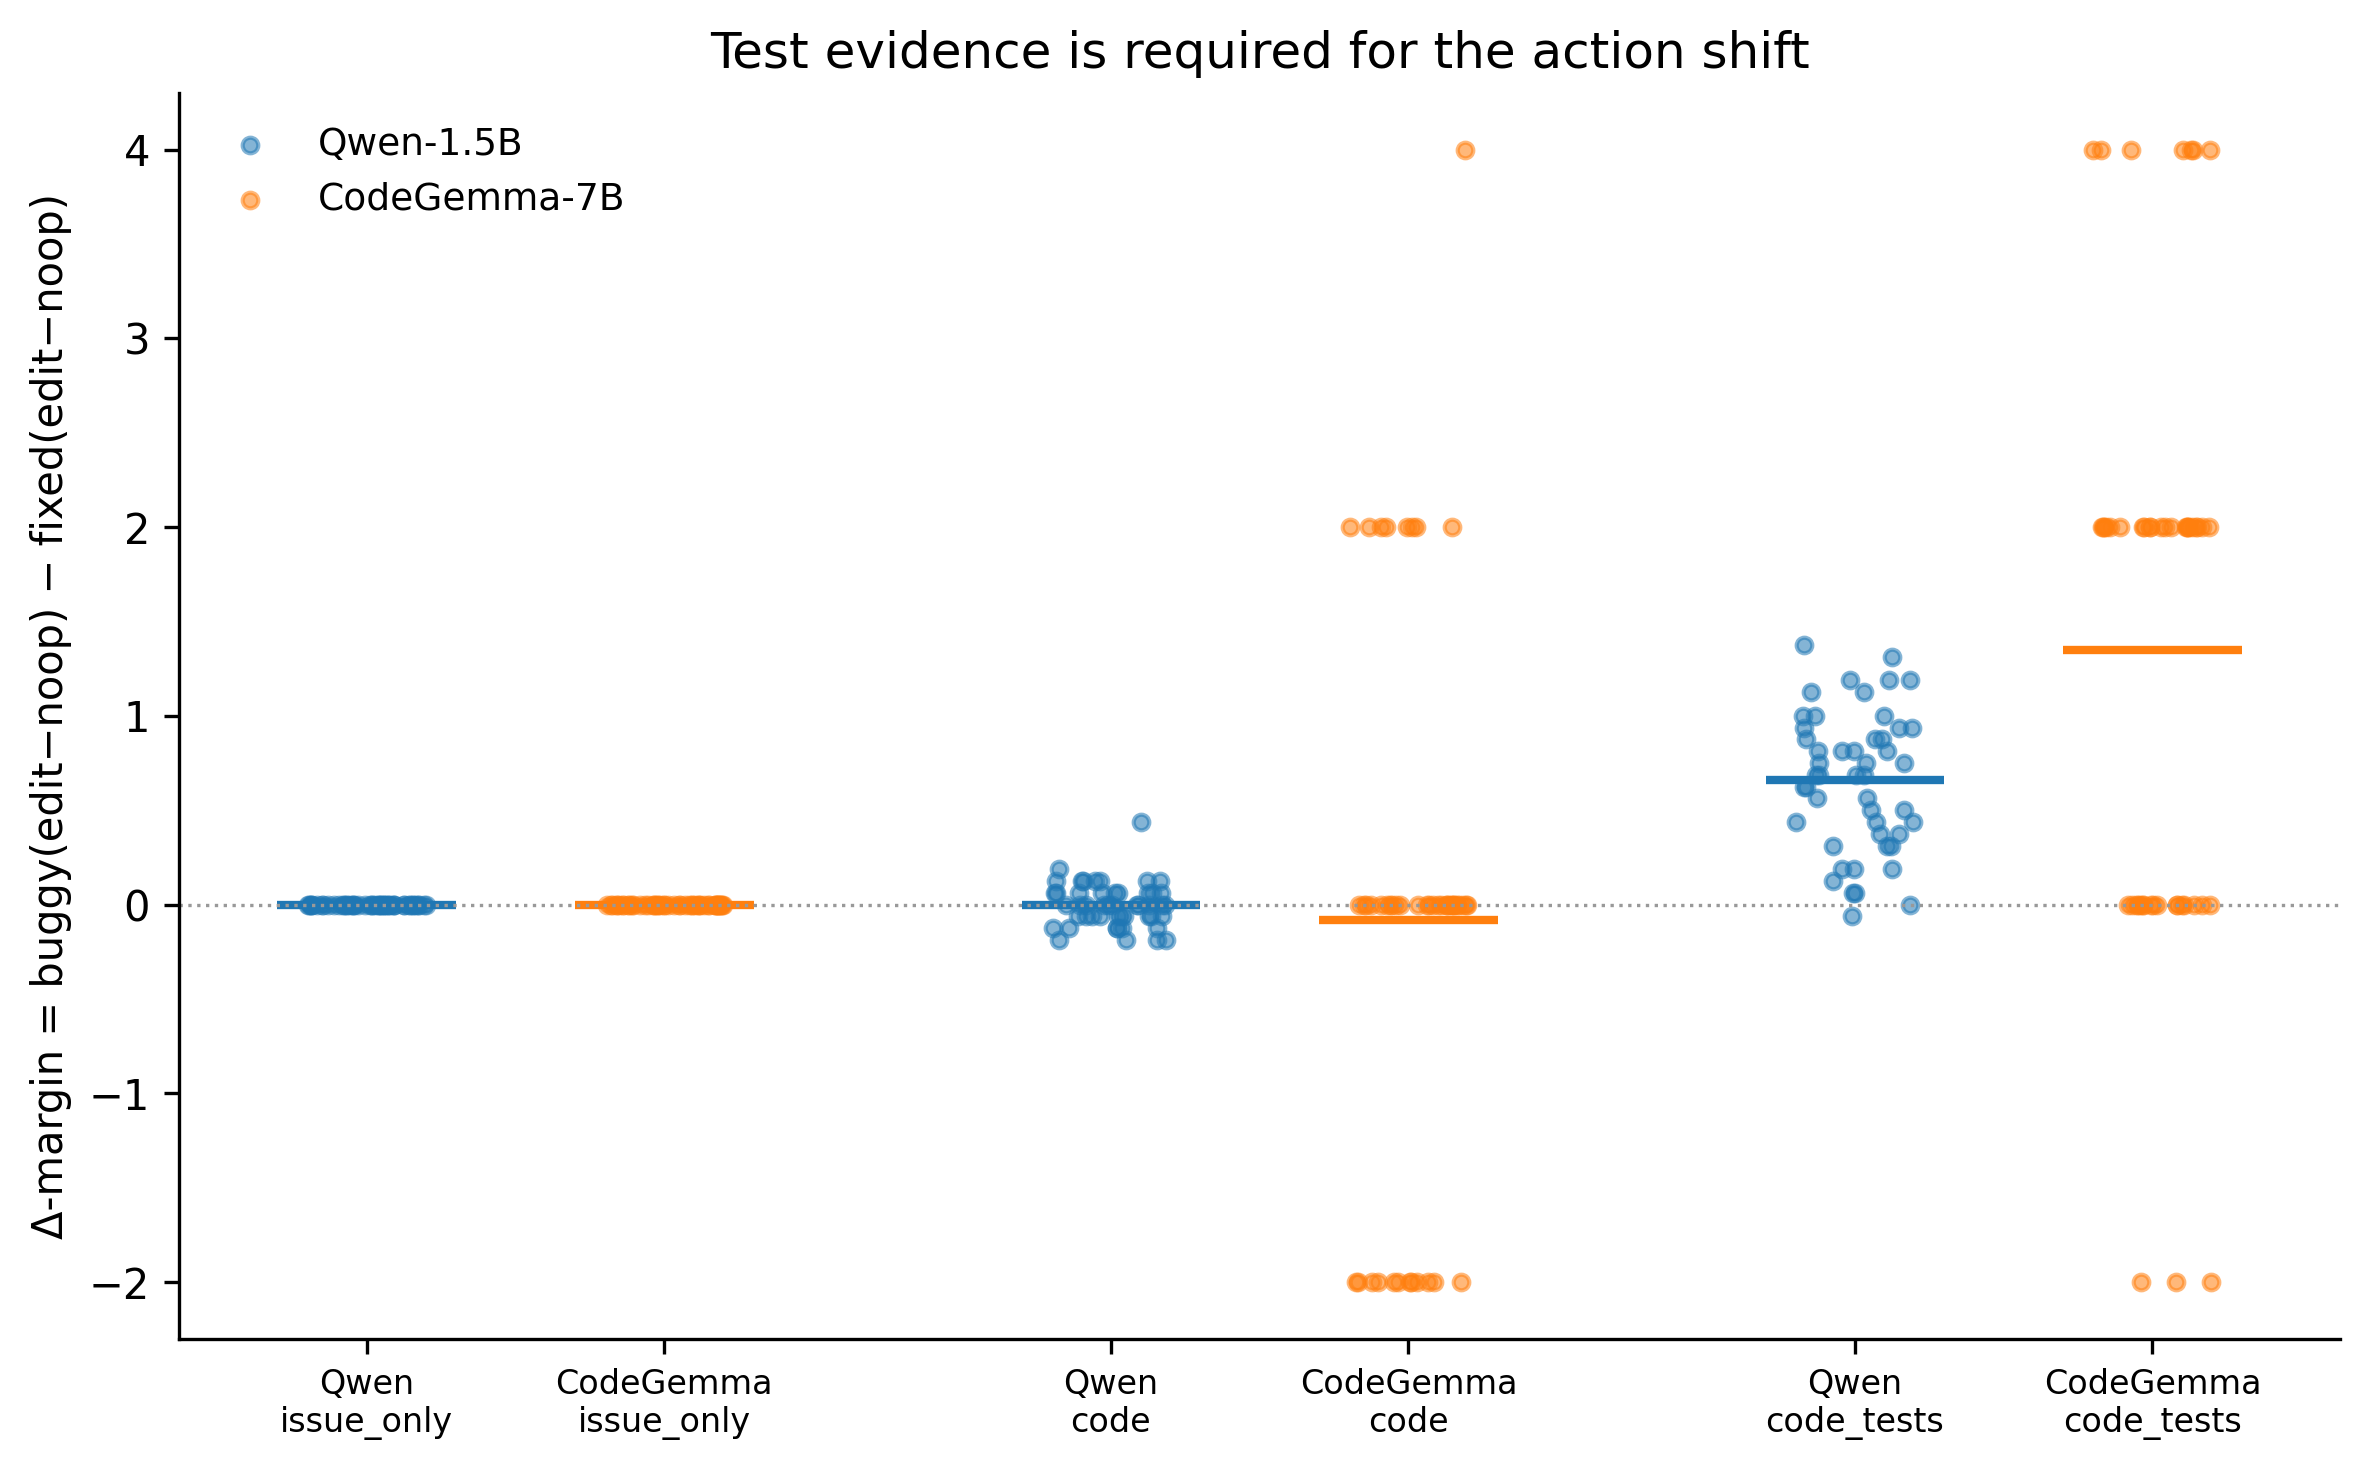
\includegraphics[width=0.9\linewidth,height=\textheight,keepaspectratio,alt={Behavioral \ensuremath{\Delta}-margin per task across three evidence levels and two models.}]{figures/behavioral_delta.png}
\caption{Behavioral \ensuremath{\Delta}-margin per task across three evidence levels and
two models.}
\end{figure}

\textbf{Probes saturate.} A logistic regression on \texttt{resid\_post}
predicting \texttt{buggy} vs \texttt{fixed} from features at any (layer,
position) achieves AUC \ensuremath{\approx} 1.0 across all 28 layers under
\texttt{code\_tests}, including layer 0 (raw embeddings). This is
uninformative on its own: the prompts contain very different surface
text (\texttt{FAILED} lines vs all-pass) and even the embedding layer
can trivially separate them. Probes confirm that the information is
widely available in the residual stream; they do not identify
\emph{where the action computation uses it}.

\section{Qwen patching heatmap, exploratory CodeGemma heatmap, and Qwen
negative
control}\label{qwen-patching-heatmap-exploratory-codegemma-heatmap-and-qwen-negative-control}

Qwen F\ensuremath{\rightarrow}B heatmap and exploratory CodeGemma F\ensuremath{\rightarrow}B heatmap:

\begin{figure}
\centering
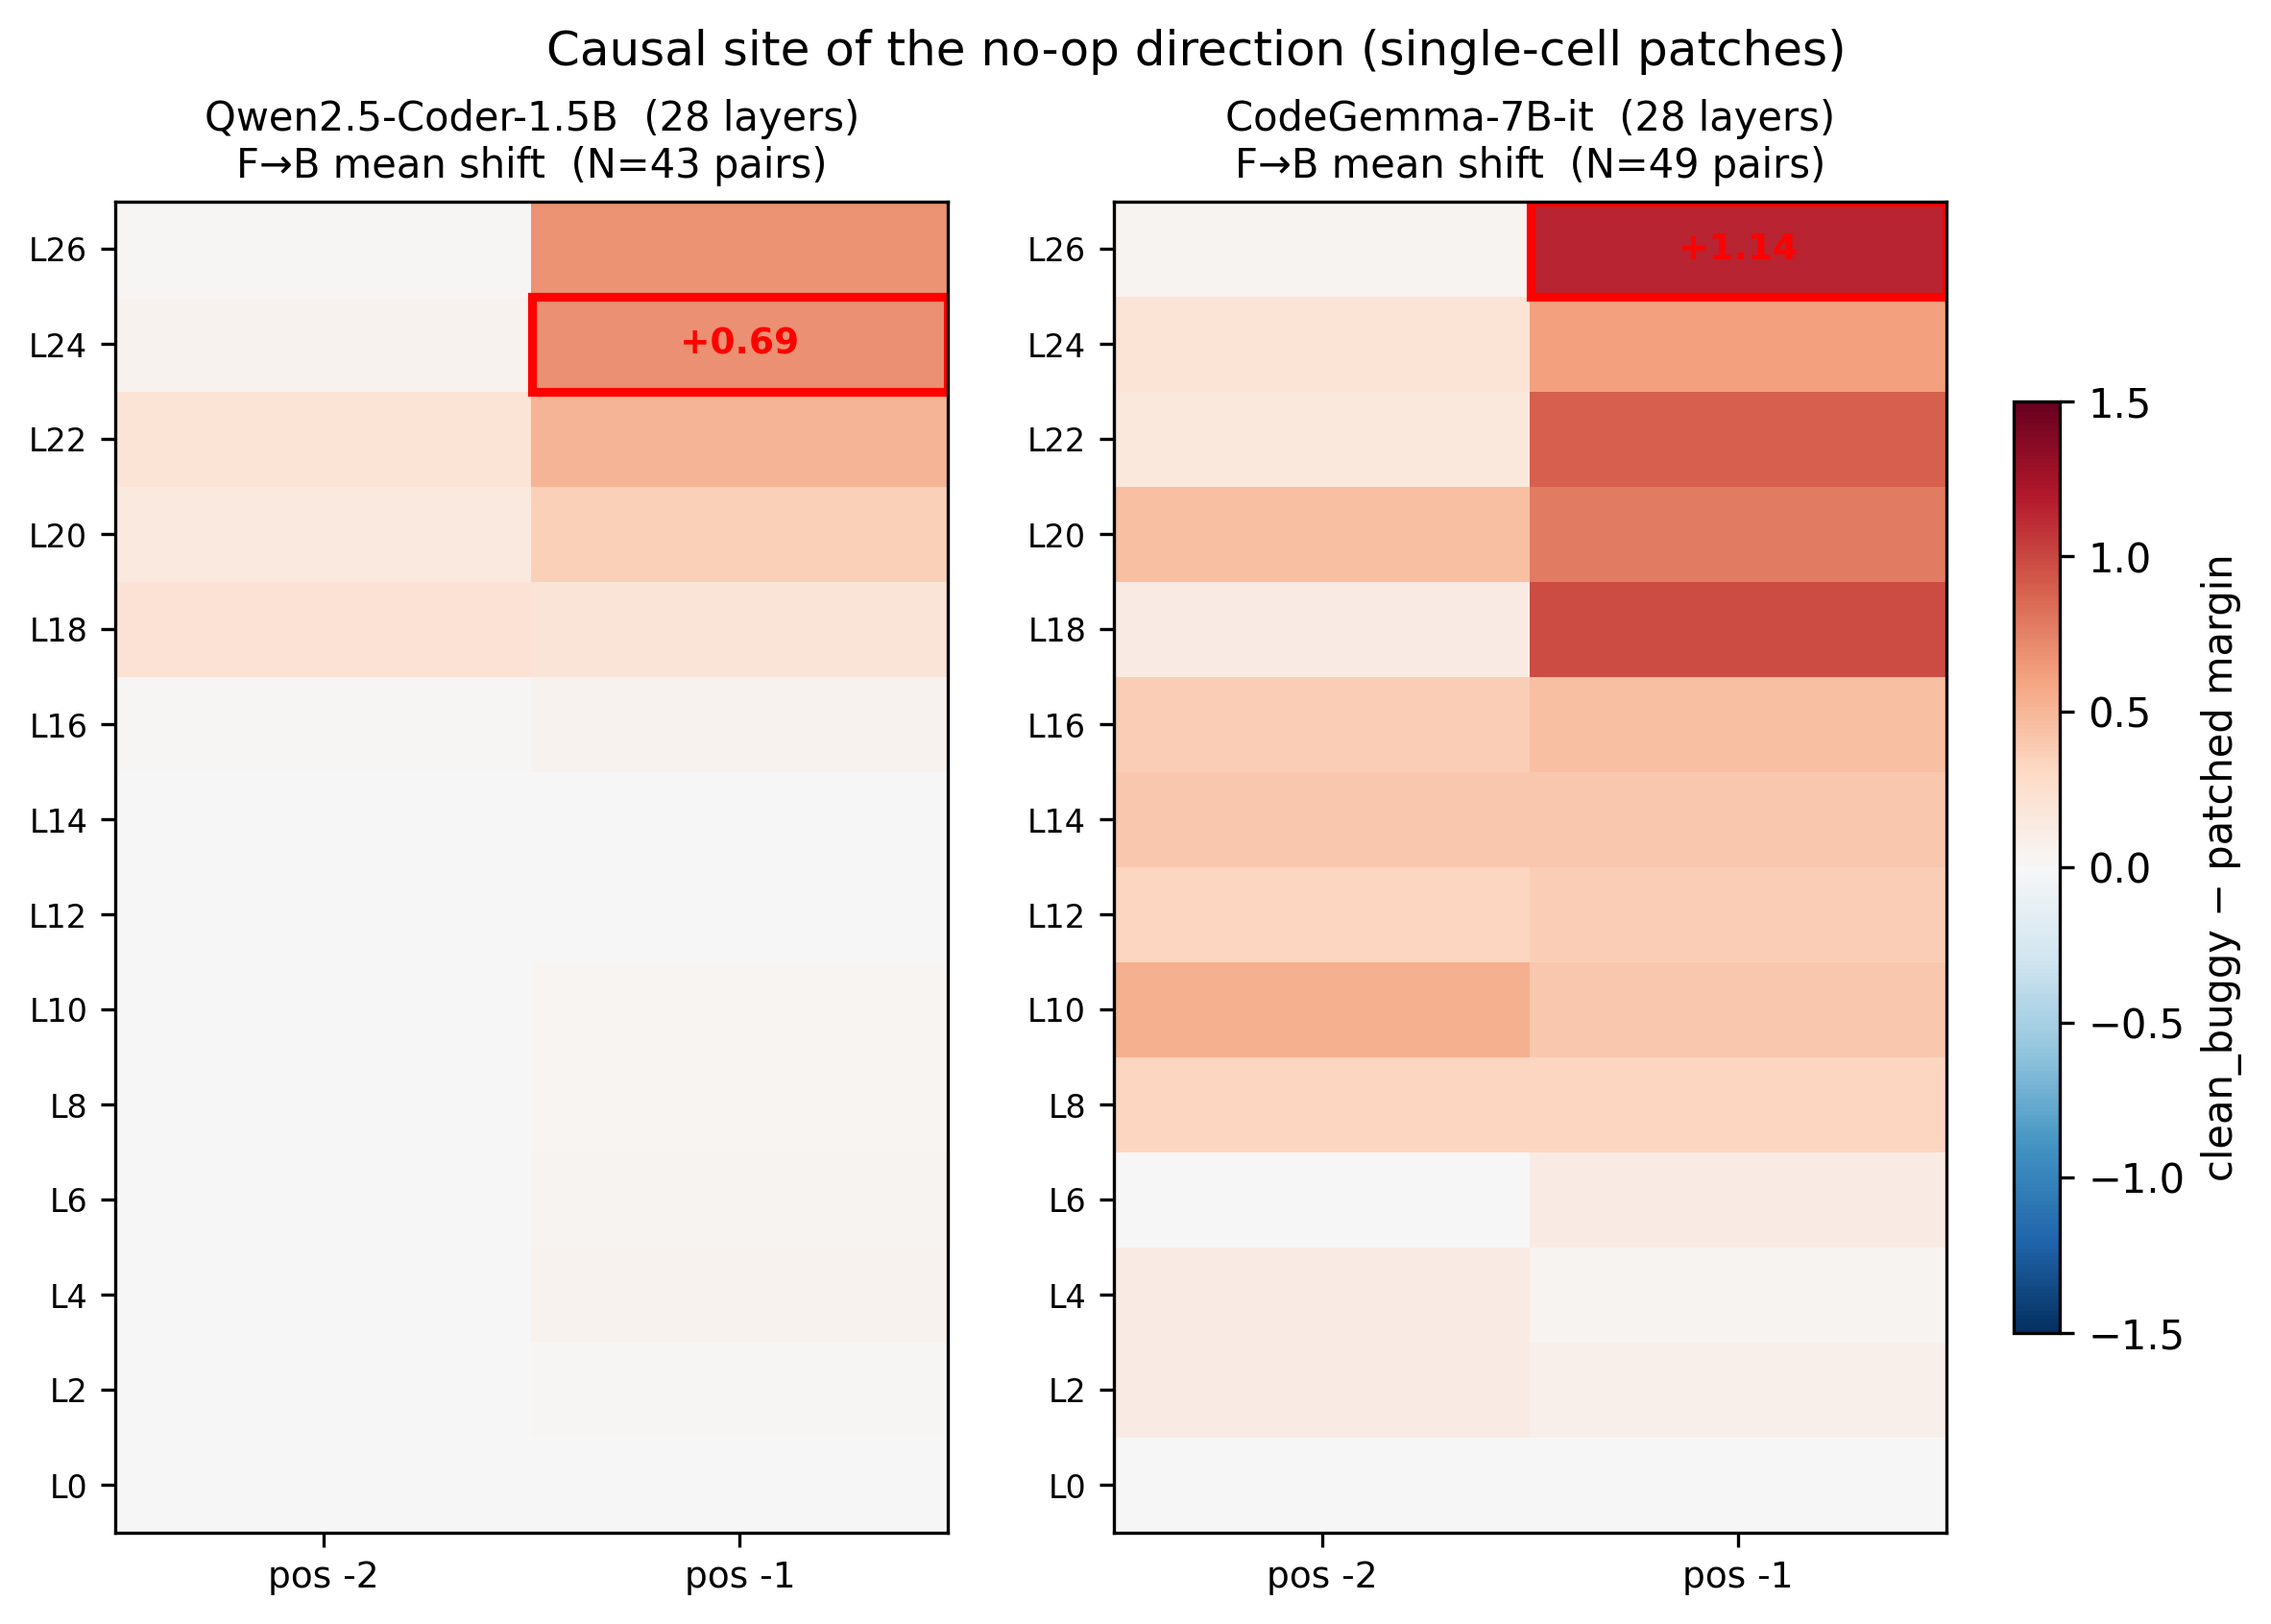
\includegraphics[width=0.92\linewidth,height=\textheight,keepaspectratio,alt={Layer \ensuremath{\times} position mean-shift heatmaps: Qwen F\ensuremath{\rightarrow}B grid (left) and exploratory CodeGemma F\ensuremath{\rightarrow}B grid (right). Only Qwen has the full bidirectional sampled grid and max-statistic permutation null; the CodeGemma panel is an exploratory one-way F\ensuremath{\rightarrow}B sweep.}]{figures/patching_heatmap.png}
\caption{Layer \ensuremath{\times} position mean-shift heatmaps: Qwen F\ensuremath{\rightarrow}B grid (left) and
exploratory CodeGemma F\ensuremath{\rightarrow}B grid (right). Only Qwen has the full
bidirectional sampled grid and max-statistic permutation null; the
CodeGemma panel is an exploratory one-way F\ensuremath{\rightarrow}B sweep.}
\end{figure}

\textbf{Specificity to test evidence.} On Qwen, the same bidirectional
patching protocol on the \texttt{code} variant (no test transcript)
shows no positive peak. At the canonical L24/pos \ensuremath{-}1 cell, F\ensuremath{\rightarrow}B mean shift
is \textbf{+0.015} (median +0.000, 45\% positive, essentially chance),
compared to +0.648 mean / +0.688 median (100\% positive) under
\texttt{code\_tests}. A small \emph{negative} cluster appears at the
very-late layers L22--L26 / pos \ensuremath{-}1 (\textasciitilde\ensuremath{-}0.18 to \ensuremath{-}0.27), in
the opposite direction of the no-op shift: substituting unrelated
residual content at this site without test-evidence routing tends to
weakly push the action toward \texttt{edit}. We interpret this as the
L24/pos \ensuremath{-}1 site being a test-evidence-conditional readout; in the
absence of an upstream pytest transcript it does not carry the
pass/fail-evidence direction at all.

\begin{figure}
\centering
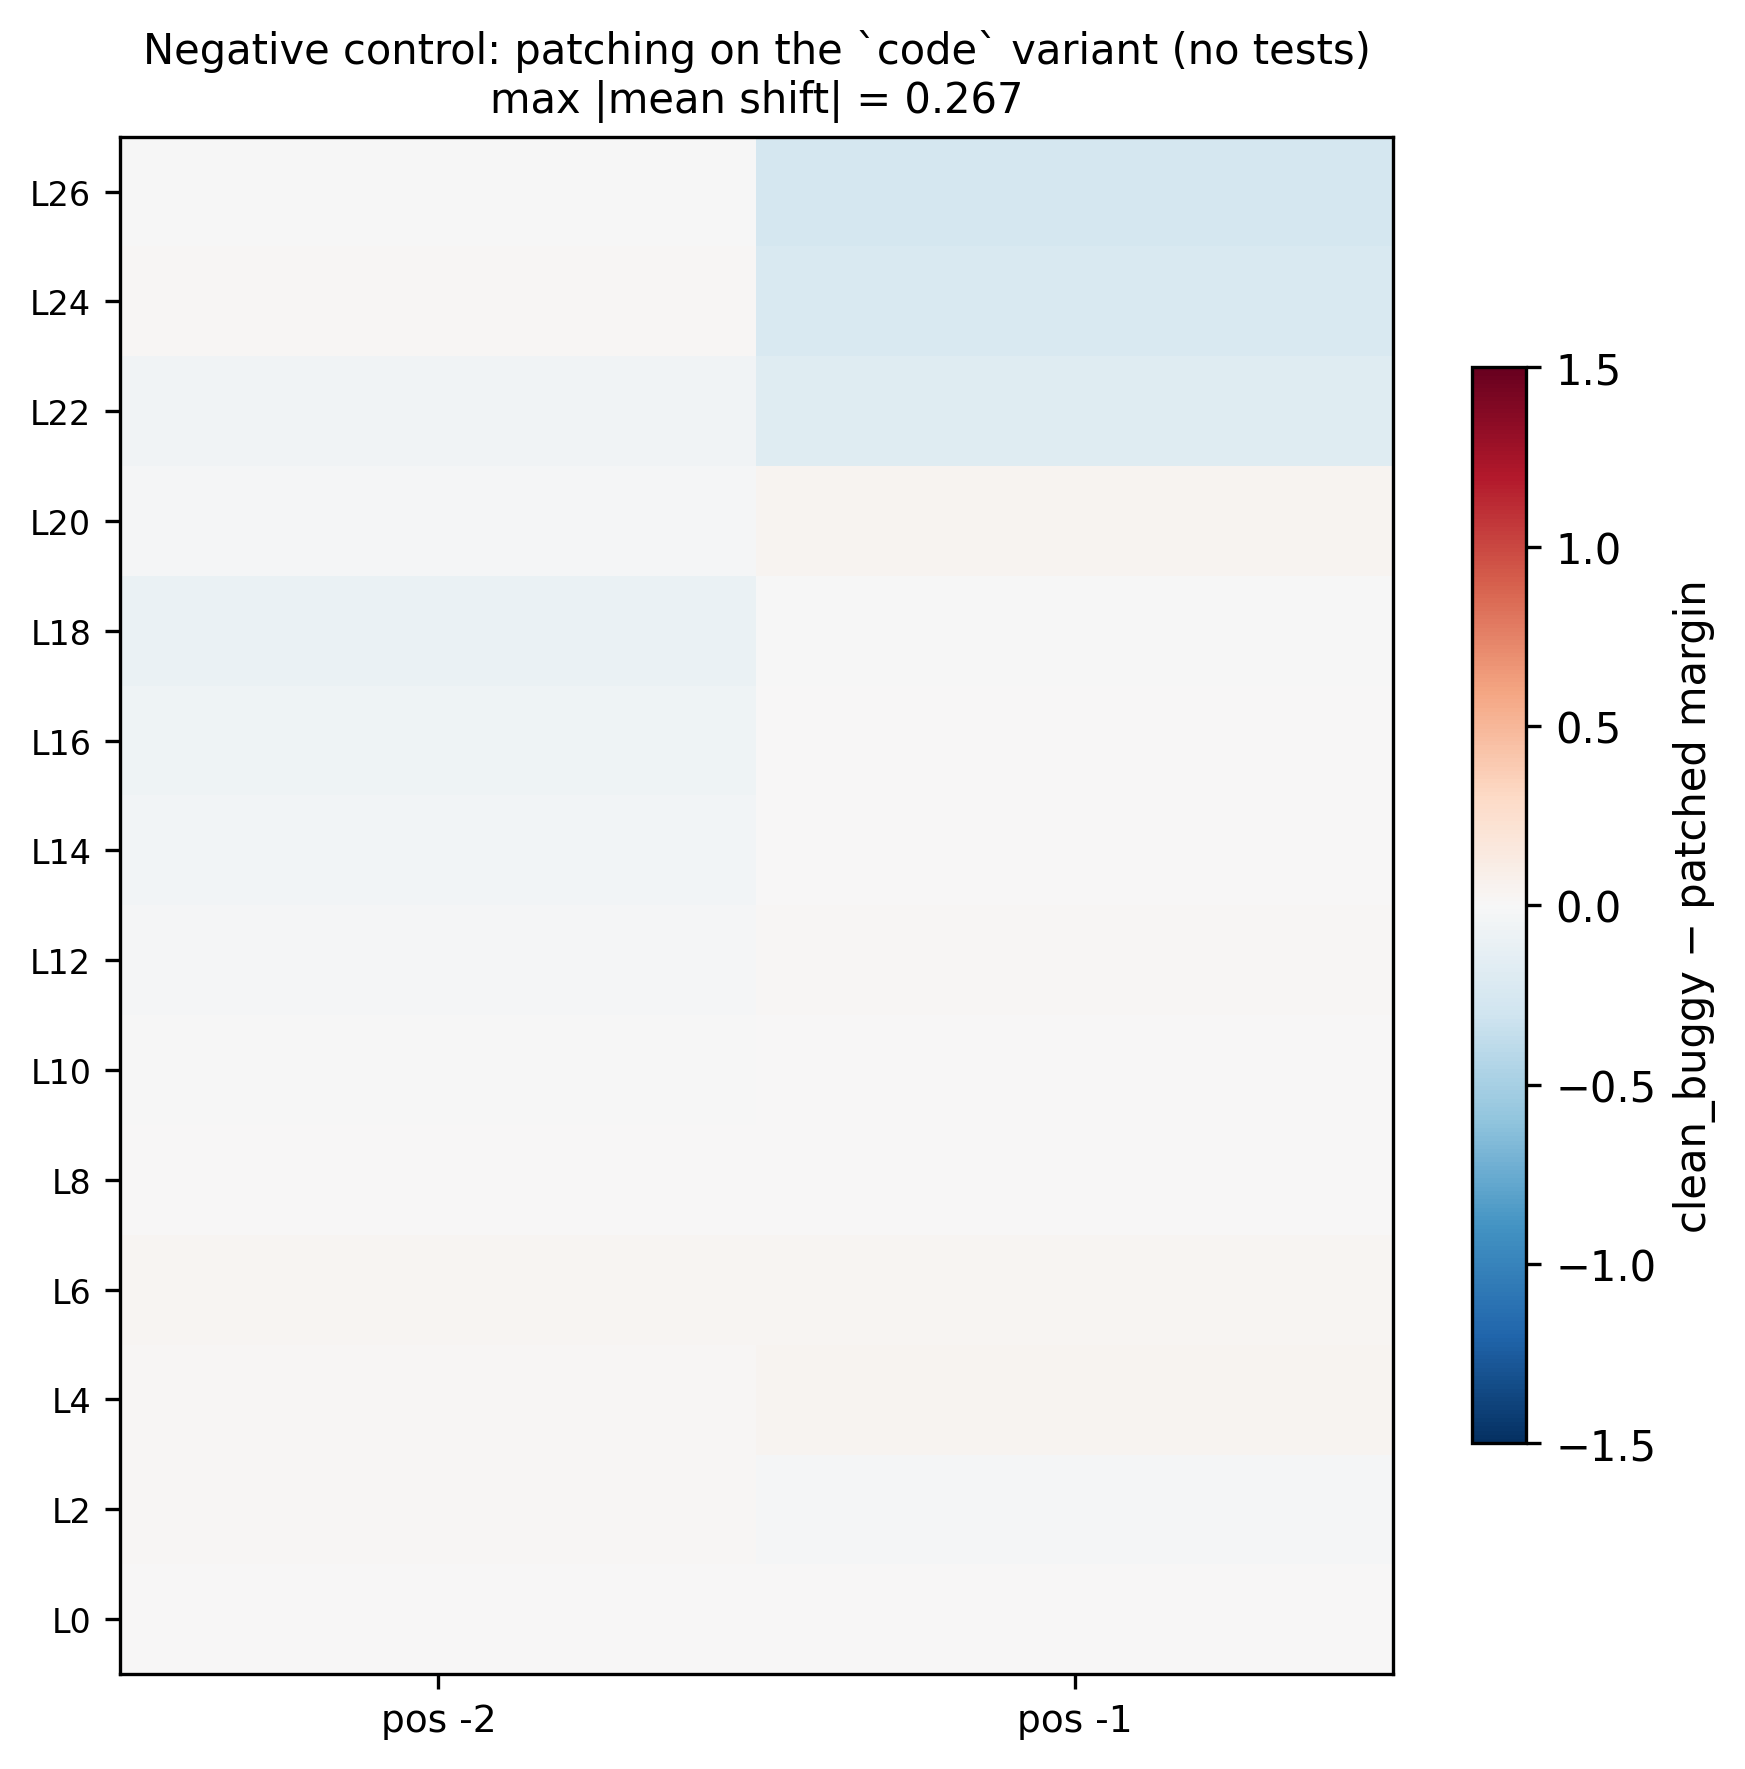
\includegraphics[width=0.6\linewidth,height=\textheight,keepaspectratio,alt={Negative-control patching on the code variant (no test transcript).}]{figures/negative_control.png}
\caption{Negative-control patching on the \protect\texttt{code} variant
(no test transcript).}
\end{figure}

\textbf{Multiple-testing correction on the grid maximum.} The Qwen
patching grid spans 14 sampled layers \ensuremath{\times} 2 positions = 28 cells;
selecting the peak via \texttt{argmax} raises the obvious question of
whether L24/pos \ensuremath{-}1 is the multiple-testing winner of sampling noise. We
address this with a max-statistic sign-flip permutation null. Under H\_0
(``at every cell the F\ensuremath{\rightarrow}B per-task shift distribution is symmetric around
zero''), multiplying each task's shift vector by an independent \ensuremath{\pm}1 sign
is exchangeable. For each of \textbf{B = 10000} permutations we redraw a
length-43 sign vector, recompute the per-cell mean shift, and record the
max across the 28 cells. The observed max (+0.6875 at L24/pos \ensuremath{-}1) is
\textbf{larger than every one of 10000 null maxima} (null mean 0.055,
null std 0.065, null 97.5th-percentile 0.228, null max 0.446; \textbf{p
\textless{} 1/10001} under the standard +1/+1 small-sample correction).
The max-statistic null distribution natively accounts for the
multiple-comparisons burden because each null draw also takes the
maximum across all 28 cells. Recipe and JSON record:
\texttt{scripts/compute\_patching\_grid\_permutation.py} \ensuremath{\rightarrow}
\texttt{results/patch\_grid\_permutation.json}.

\section{Steering dose-response per-task
curves}\label{steering-dose-response-per-task-curves}

Per-task dose-response across \ensuremath{\alpha} \ensuremath{\in} \{\ensuremath{-}3, \ldots, +3\}, Qwen + CodeGemma
overlay:

\begin{figure}
\centering
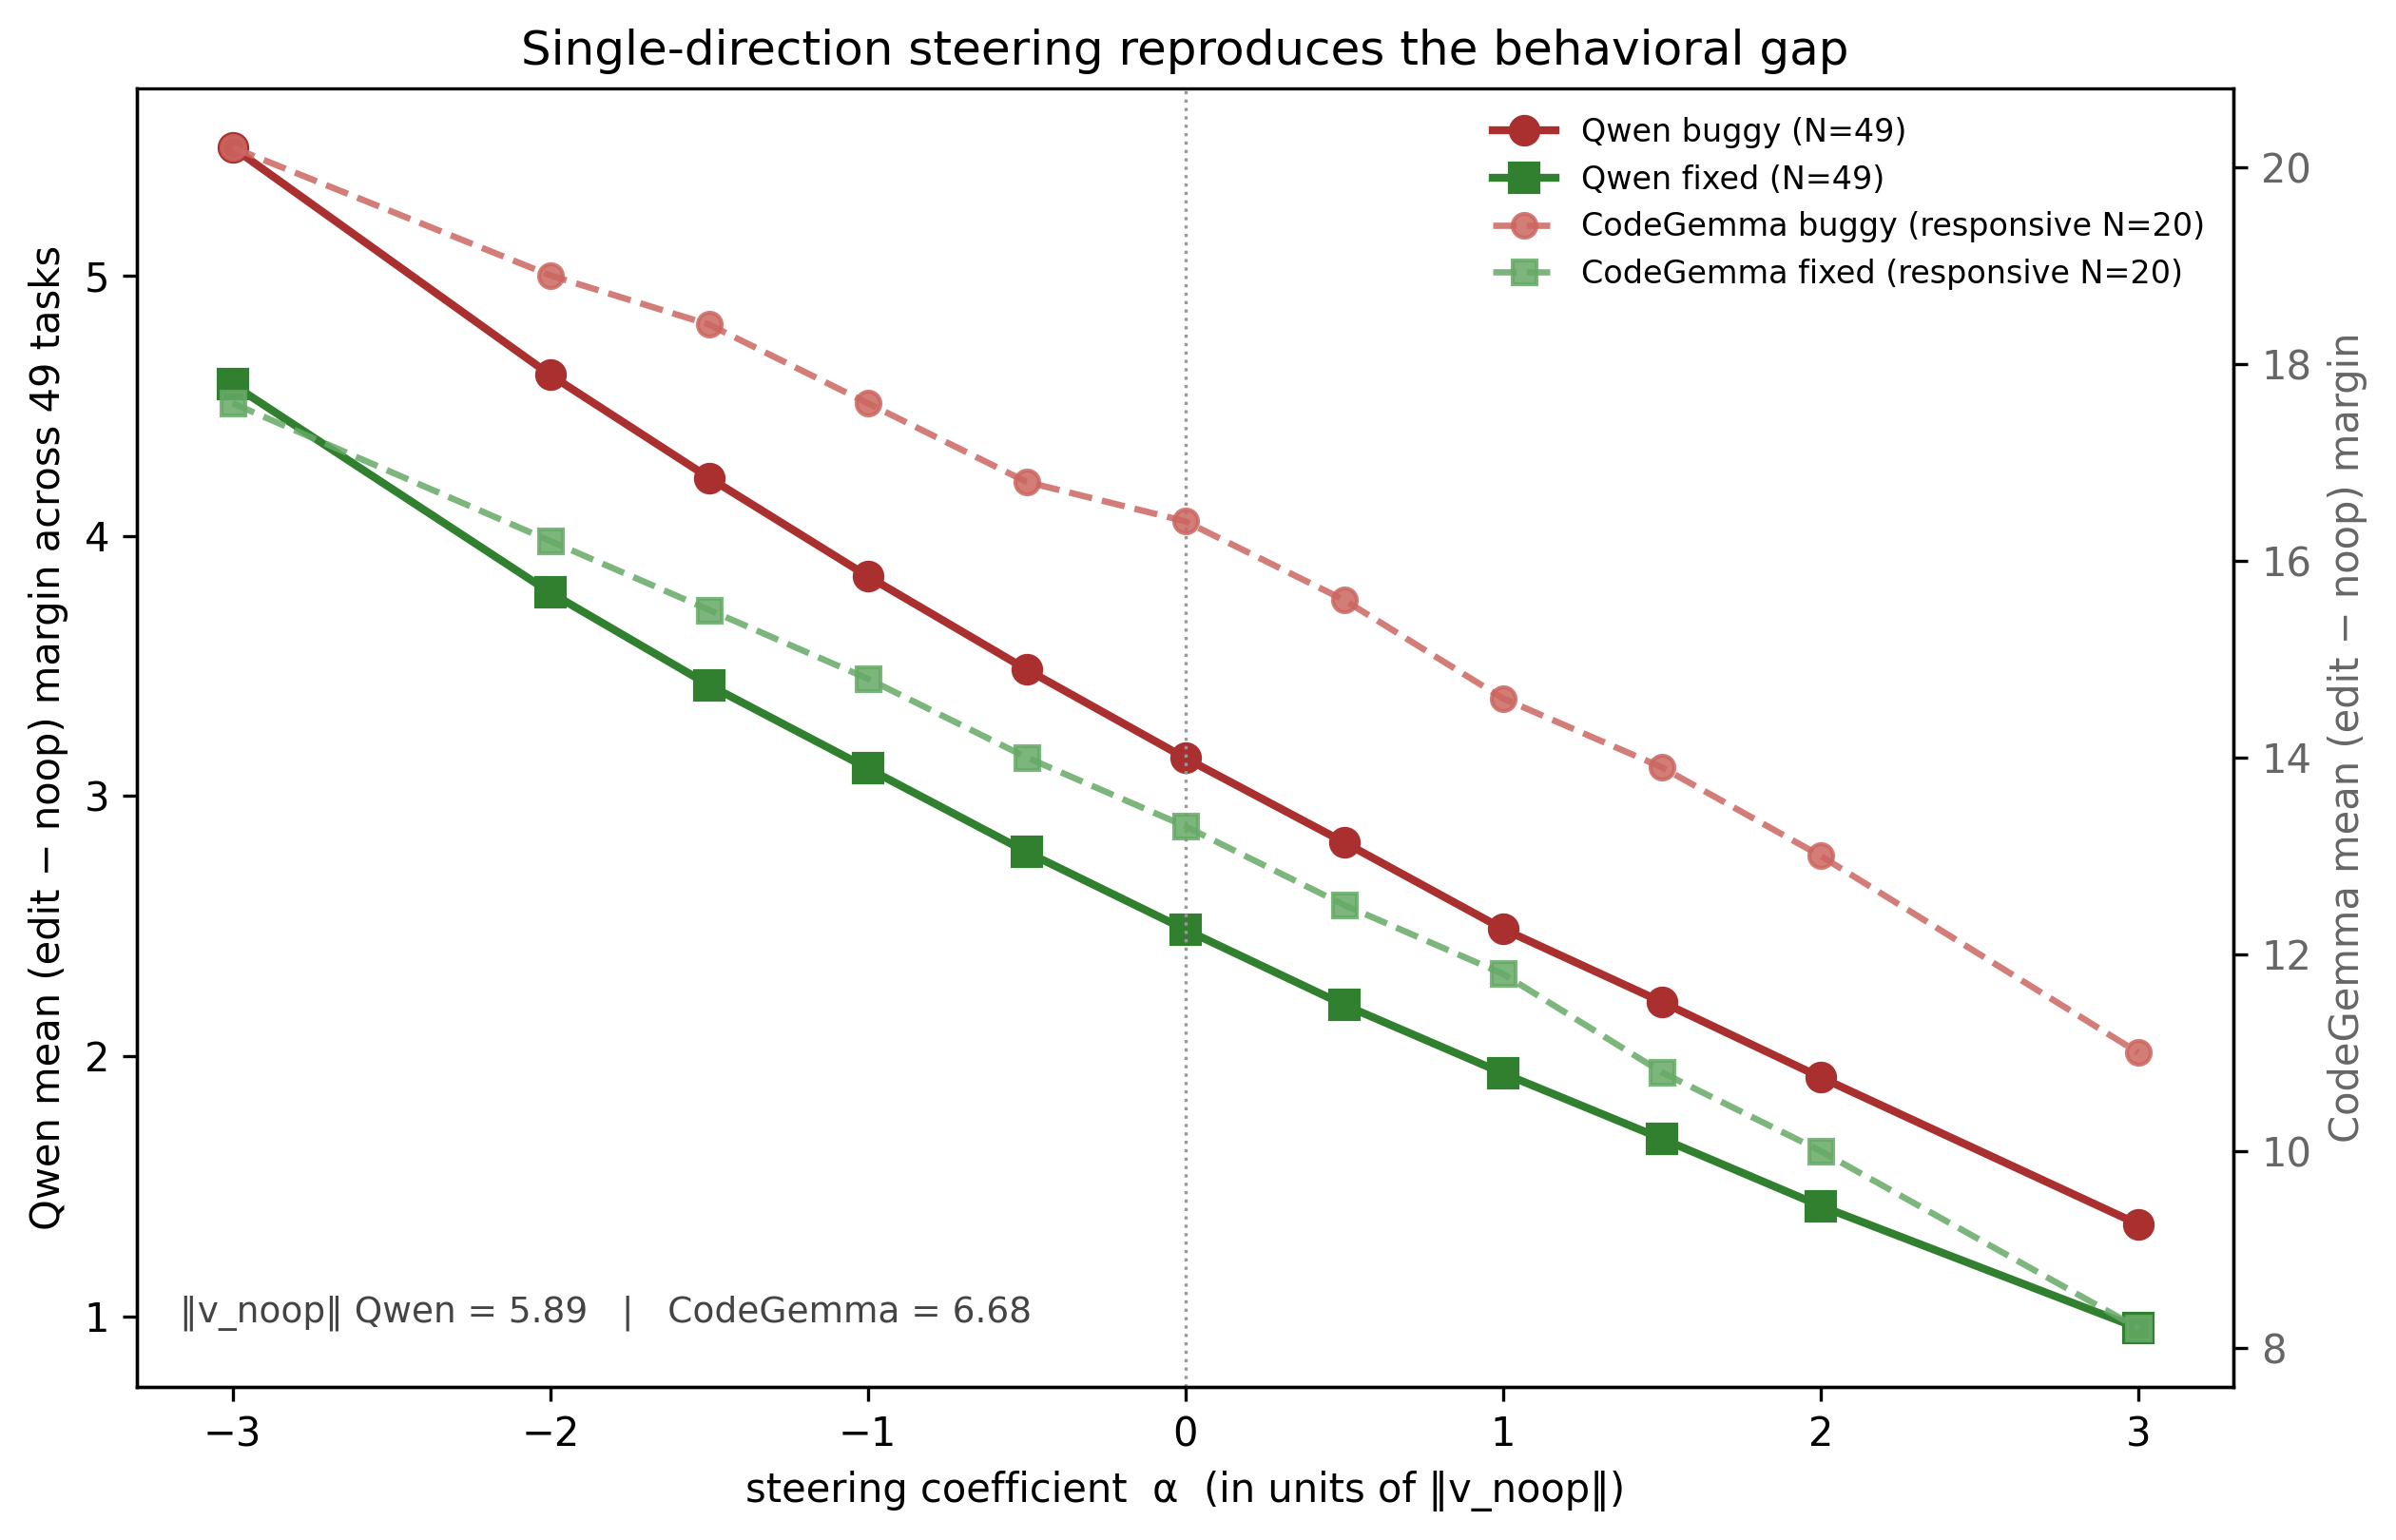
\includegraphics[width=0.9\linewidth,height=\textheight,keepaspectratio,alt={Single-direction steering dose-response curves; Qwen full N=49 (solid), CodeGemma responsive subset N=20 (dashed, right y-axis).}]{figures/steering_dose_response.png}
\caption{Single-direction steering dose-response curves; Qwen full N=49
(solid), CodeGemma responsive subset N=20 (dashed, right y-axis).}
\end{figure}

This is a stronger claim than patching: patching replaces a 1536-dim
vector; steering shows the same \texttt{edit\ \ensuremath{-}\ noop} margin shift can
be reproduced by a single rank-1 additive intervention along the raw
contrastive vector \(v_{\rm raw}\). \textbf{A single labeled contrastive
direction is sufficient to steer the margin under our
code-plus-transcript prompt distribution.} This does not establish that
pass/fail-transcript information is uniquely one-dimensional or absent
from higher-rank subspaces (PCA1 at the same cell is comparable in \S{}G.2,
and probes saturate at every layer); \(u_{\rm tx}\) is the
\emph{labeled} direction that comes for free from paired-task mean
differences and works directly under additive intervention.

\section{Stale-variant failure analysis and toy-monitor
LOOCV}\label{stale-variant-failure-analysis-and-toy-monitor-loocv}

\begin{figure}
\centering
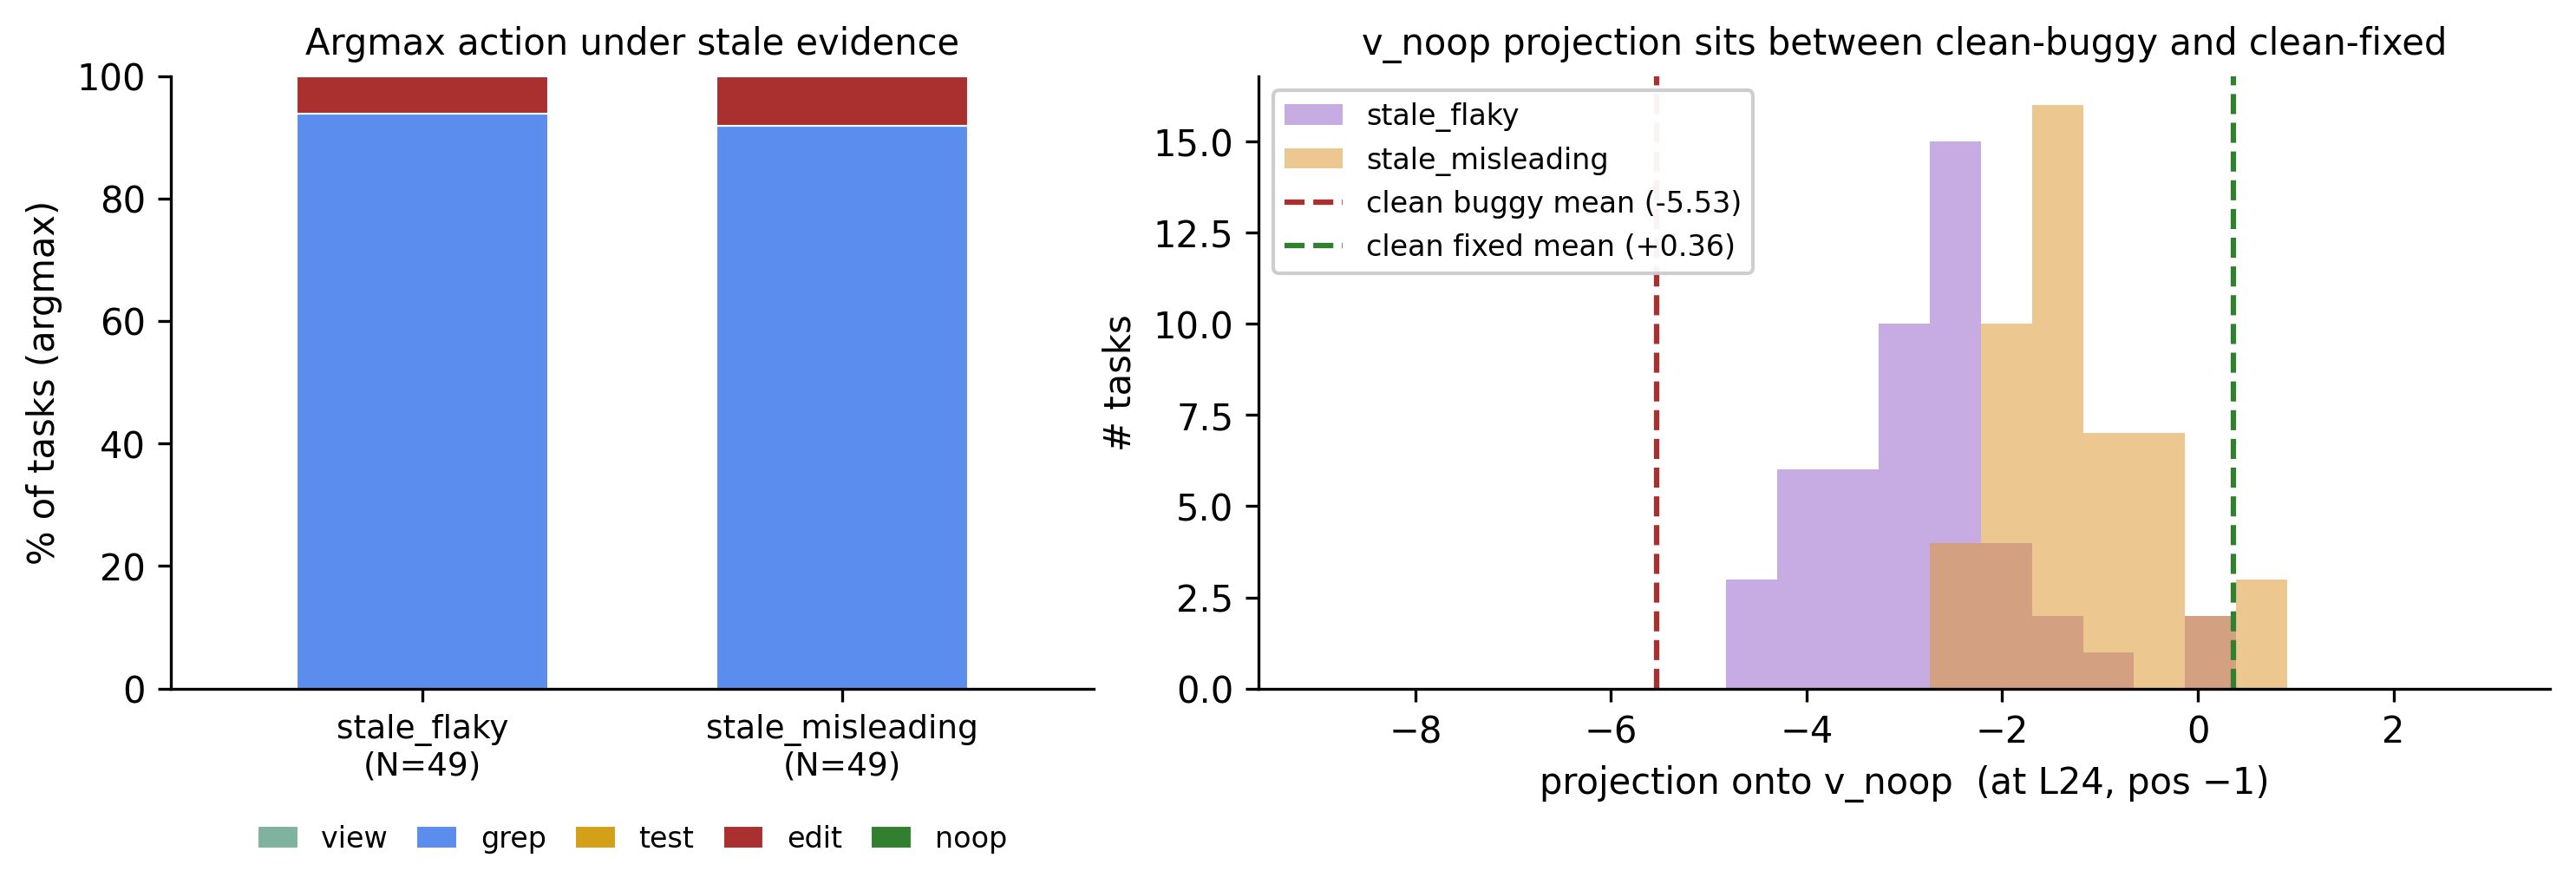
\includegraphics[width=0.92\linewidth,height=\textheight,keepaspectratio,alt={Failure analysis under stale evidence (Qwen, N=49 per variant).}]{figures/failure_table.png}
\caption{Failure analysis under stale evidence (Qwen, N=49 per
variant).}
\end{figure}

A monitor that thresholds the classifier score \(s=-h\cdot u_{\rm tx}\)
converts the latent pass/fail-transcript signal into an overt
transcript-based fixed/passing label under this prompt format, not an
independent abstention/no-edit decision (the model itself does not emit
\texttt{noop} at first-token argmax). Under leave-one-out CV on the 49
clean buggy/fixed pairs the monitor achieves ROC-AUC = 1.000 and AP =
1.000, with 100\% precision and 100\% recall at the balanced-accuracy
operating point. A permutation null over 1000 label-shuffled LOOCV runs
(seed=0, \texttt{scripts/compute\_auc\_cis.py}) puts the observed AUC of
1.000 at the 100th percentile of the null distribution (null mean 0.501,
max 0.660, p = 0.001), the LOOCV result is not a small-N coincidence. We
do not claim this clean separation persists on stale-evidence prompts
(where the latent projection compresses toward zero); a thresholded toy
projection uses the threshold learned on clean pairs to flag prompts
whose classifier score falls into the fixed/passing region. Under this
prompt format, that score can be interpreted as a post-hoc
transcript-based fixed/passing label even when the model's own
first-token argmax is not \texttt{noop}.

\begin{figure}
\centering
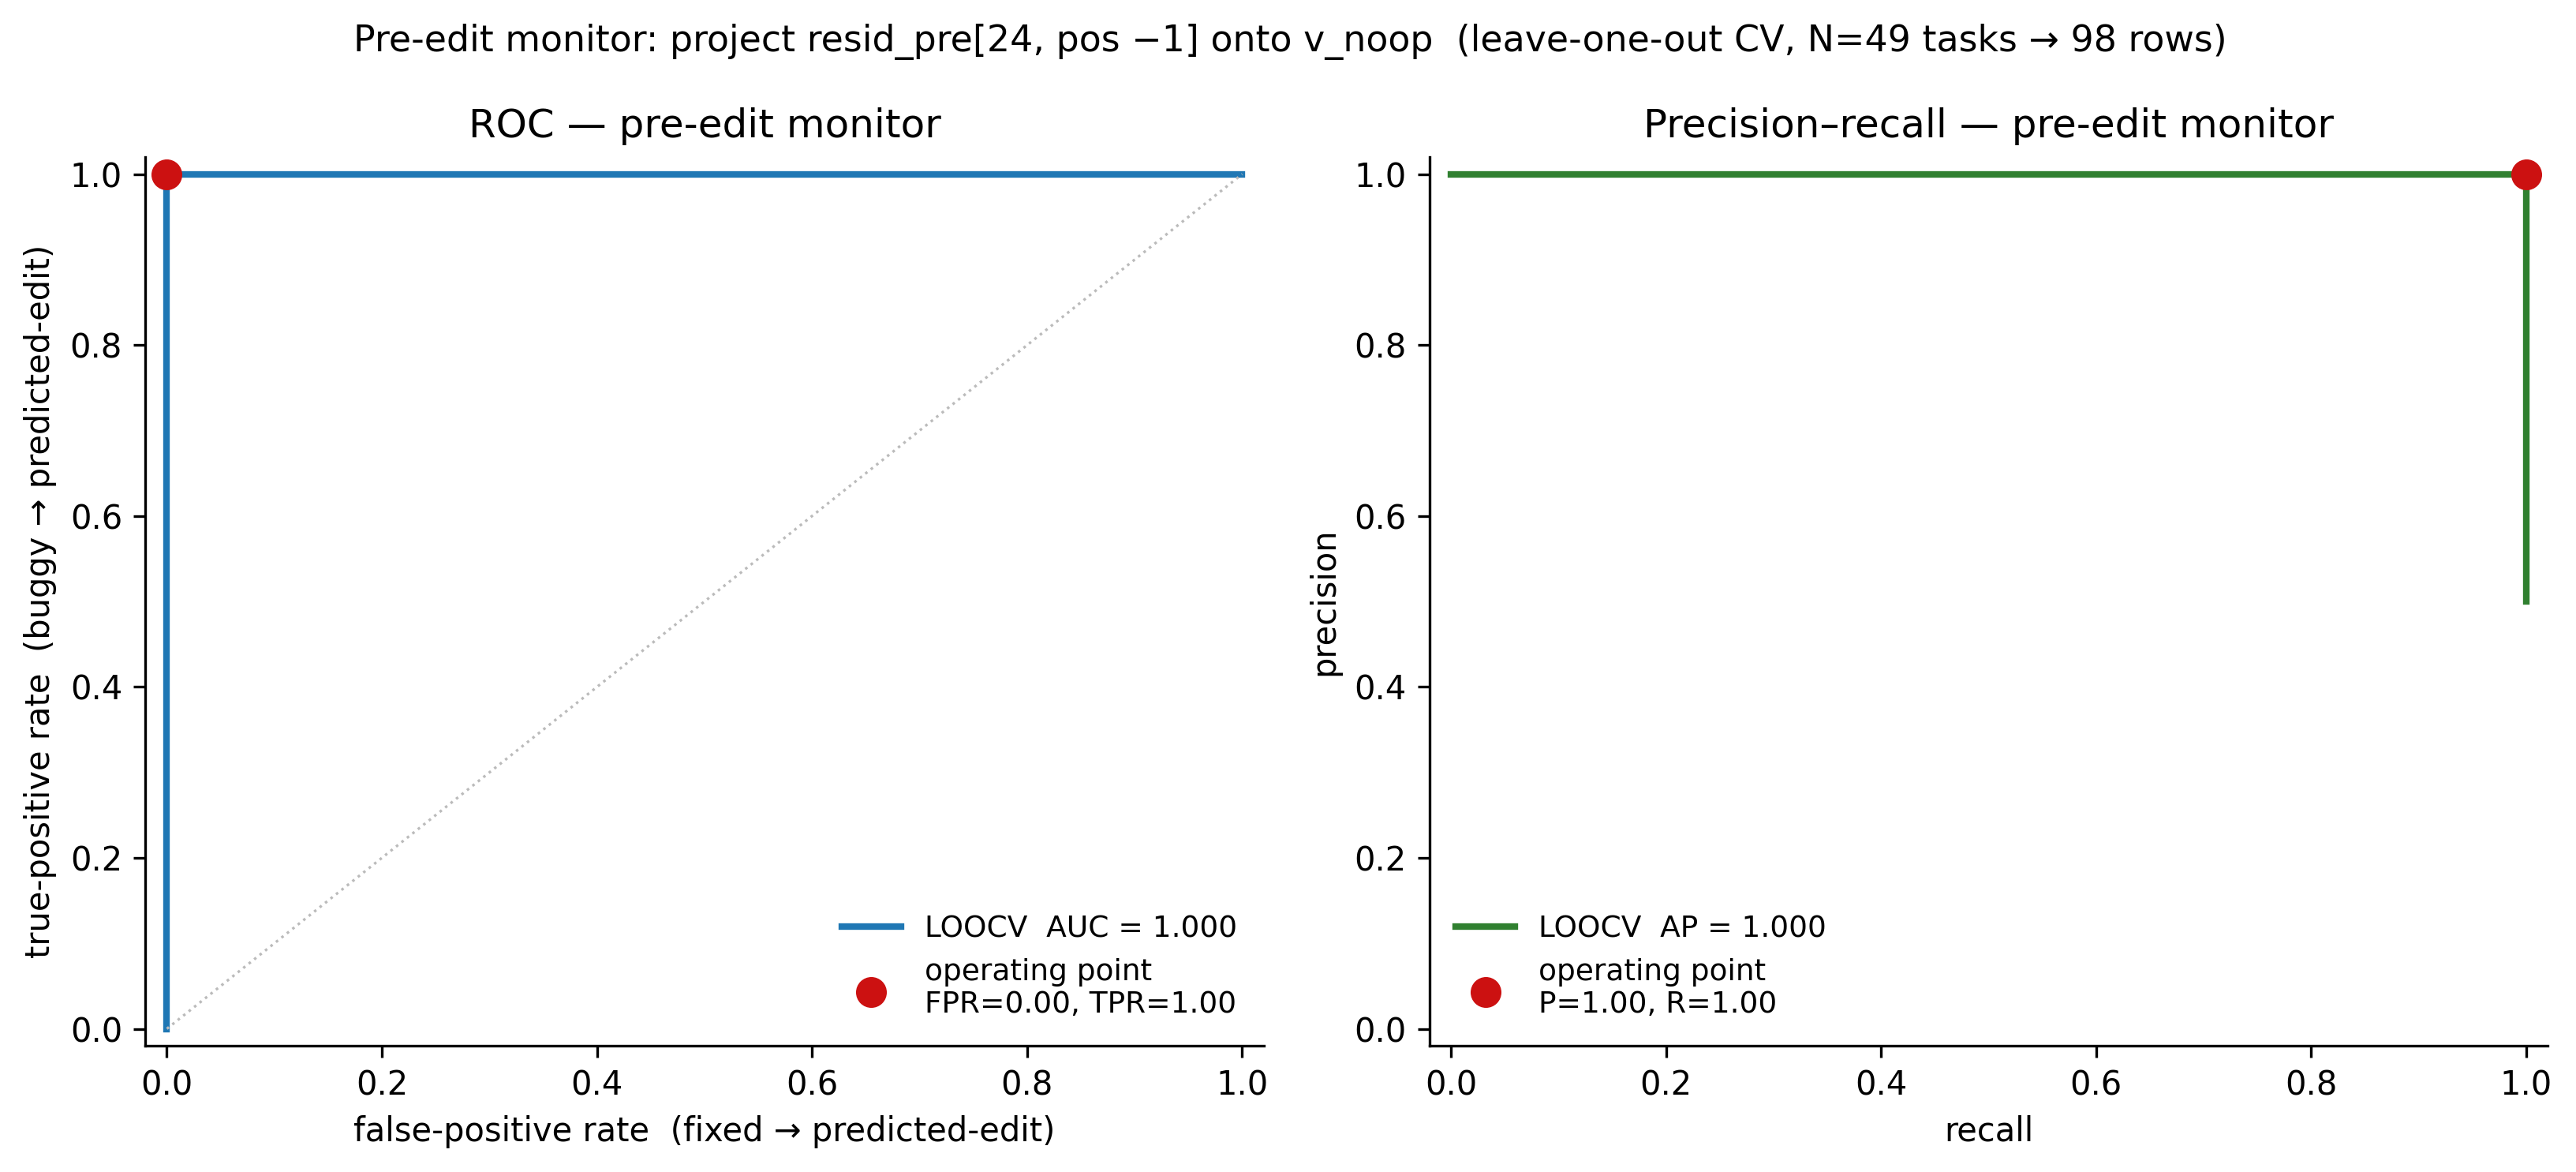
\includegraphics[width=0.92\linewidth,height=\textheight,keepaspectratio,alt={Transcript-label projection monitor, ROC and precision-recall under leave-one-out CV (toy substrate).}]{figures/monitor_roc.png}
\caption{Transcript-label projection monitor, ROC and precision-recall
under leave-one-out CV (toy substrate).}
\end{figure}

\section{SWE-derived evaluation: full per-task tables and
baselines}\label{swe-derived-evaluation-full-per-task-tables-and-baselines}

\subsection{SWE-derived ingestion and projection
statistics}\label{swe-derived-ingestion-and-projection-statistics}

The SWE-bench-Verified-\emph{derived} paired-prompt evaluation was
conducted on 499 / 497 / 499 instances (Qwen / CodeGemma / DeepSeek; 1
instance dropped at ingestion because its modified file no longer exists
at the base commit; 2 additional CodeGemma instances dropped for
exceeding a 2400-token cap needed to avoid A10G OOM on the 7B model).
This is a static-classifier evaluation, \textbf{not} the official
SWE-bench agent evaluation \citep{jimenez2024swebench} (no patch
generation, no test execution, no repository access). Each instance was
ingested using a deterministic script extracting an 80-line window
around the gold patch's largest Python hunk, applying the hunk in-memory
to derive the fixed counterpart, and synthesizing a pytest transcript
from the dataset's \texttt{FAIL\_TO\_PASS} and \texttt{PASS\_TO\_PASS}
lists (no Docker / pytest execution required).

Projecting \texttt{resid\_pre} at each model's toy-trained intervention
site onto its unit monitor direction \(u_{\rm tx}\) (projection
\(p=h\cdot u_{\rm tx}\), lower = failing-transcript; gap = mean-fixed \ensuremath{-}
mean-buggy):

{\def\LTcaptype{none} % do not increment counter
\begin{longtable}[]{@{}
  >{\raggedright\arraybackslash}p{(\linewidth - 10\tabcolsep) * \real{0.3293}}
  >{\raggedright\arraybackslash}p{(\linewidth - 10\tabcolsep) * \real{0.1829}}
  >{\raggedright\arraybackslash}p{(\linewidth - 10\tabcolsep) * \real{0.1707}}
  >{\raggedright\arraybackslash}p{(\linewidth - 10\tabcolsep) * \real{0.1341}}
  >{\raggedright\arraybackslash}p{(\linewidth - 10\tabcolsep) * \real{0.1341}}
  >{\raggedright\arraybackslash}p{(\linewidth - 10\tabcolsep) * \real{0.0488}}@{}}
\toprule\noalign{}
\begin{minipage}[b]{\linewidth}\raggedright
condition / source
\end{minipage} & \begin{minipage}[b]{\linewidth}\raggedright
model
\end{minipage} & \begin{minipage}[b]{\linewidth}\raggedright
layer/pos
\end{minipage} & \begin{minipage}[b]{\linewidth}\raggedright
mean \(p\)
\end{minipage} & \begin{minipage}[b]{\linewidth}\raggedright
fixed\ensuremath{-}buggy gap
\end{minipage} & \begin{minipage}[b]{\linewidth}\raggedright
N
\end{minipage} \\
\midrule\noalign{}
\endhead
\bottomrule\noalign{}
\endlastfoot
SWE-derived buggy & Qwen-1.5B & L24 / pos \ensuremath{-}1 & \textbf{\ensuremath{-}2.18} & -- &
499 \\
SWE-derived fixed & Qwen-1.5B & L24 / pos \ensuremath{-}1 & \textbf{+2.56} &
\textbf{+4.73} & 499 \\
SWE-derived buggy & CodeGemma-7B & L26 / pos \ensuremath{-}1 & \textbf{\ensuremath{-}10.85} & -- &
497 \\
SWE-derived fixed & CodeGemma-7B & L26 / pos \ensuremath{-}1 & \textbf{\ensuremath{-}7.98} &
\textbf{+2.87} & 497 \\
SWE-derived buggy & DeepSeek-1.3B & L22 / pos \ensuremath{-}1 & \textbf{+13.16} & --
& 499 \\
SWE-derived fixed & DeepSeek-1.3B & L22 / pos \ensuremath{-}1 & \textbf{+18.81} &
\textbf{+5.64} & 499 \\
Toy clean-buggy reference & Qwen-1.5B & L24 / pos \ensuremath{-}1 & \ensuremath{-}5.53 & -- &
49 \\
Toy clean-fixed reference & Qwen-1.5B & L24 / pos \ensuremath{-}1 & +0.36 & +5.89 &
49 \\
\end{longtable}
}

On a 99-pair subset the two-model monitor scores AUC 0.993 (Qwen) /
0.958 (CodeGemma); on the full benchmark these regress modestly (\ensuremath{\Delta}
\ensuremath{-}0.004 Qwen / \ensuremath{-}0.008 CodeGemma under the all-49 direction) to the \S{}5.1
headline values as the broader distribution surfaces more edge cases.

\subsection{Monitor-direction baselines: contrastive direction at the
causal cell, signal everywhere
else}\label{monitor-direction-baselines-contrastive-direction-at-the-causal-cell-signal-everywhere-else}

Two original specificity controls on Qwen at the same site (L24, pos \ensuremath{-}1,
SWE-bench-Verified-derived N=99):

\begin{itemize}
\tightlist
\item
  \textbf{Random unit-direction baseline (N = 1000).} Drawing N = 1000
  unit vectors uniformly on the 1535-sphere at (L24, pos \ensuremath{-}1) and
  computing the \textbar AUC\textbar{} each one attains as a
  signed-projection classifier yields a random-AUC distribution with
  mean 0.702, p95 0.916, p99 0.953, and max 0.983 (over all 1000 draws).
  \textbf{\(u_{\rm tx}\)'s 0.993 sits at the 100th percentile}: it beats
  every one of 1000 random directions. The random-direction max (0.983)
  is a stricter ceiling than the p99 and is still below \(u_{\rm tx}\),
  so the gap is not a chance artifact.
\item
  \textbf{Full-residual probe (1536 parameters, LOOCV).} A logistic-
  regression probe trained on the full 1536-D residual at (L24, pos \ensuremath{-}1)
  under leave-one-out CV over the 99 paired tasks reaches \textbf{ROC-
  AUC = 1.000} (likewise at L27/pos \ensuremath{-}1). \(u_{\rm tx}\)'s 1-D projection
  captures essentially all of the information the full-residual probe
  uses: 0.993 vs 1.000 (caveat: with d = 1536 \ensuremath{\gg} n = 99 the LR probe has
  substantial in-LOOCV overfitting risk, so 1.000 is an upper bound on
  what's mechanistically separable; \(u_{\rm tx}\)'s 0.993 with one
  degree of freedom is a much tighter claim).
\end{itemize}

These together imply that on the N=99 subset, \textbf{\(u_{\rm tx}\),
the labeled direction the contrastive mean-difference recipe produces,
is nearly as discriminative at the L24/pos \ensuremath{-}1 causal cell as a
full-residual probe at the same site, despite using no fitted
SWE-derived parameters}. We avoid stronger ``information-equivalent to a
1536-parameter probe'' phrasing: the probe is high-dimensional with
in-LOOCV overfitting risk, the N=99 subset is small, and the wrong-layer
/ transcript controls below weaken any ``privileged readout'' framing.
The adversarial baselines added below (wrong-layer same-position is
comparably strong, wrong-position collapses) clarify that the
localization claim is the patching peak (\S{}4.1), and the readout-quality
claim at that cell rather than a unique discriminative axis in residual
space.

\textbf{Adversarial baselines on the full N=499
SWE-bench-Verified-derived evaluation.} The random-unit-vector baseline
is intentionally weak (uniform vectors on a 1535-sphere are
near-orthogonal to any discriminative axis). We add three harder
controls on Qwen using the same paired-bootstrap methodology as \S{}5.1
(B=10000, seed=0; \texttt{scripts/adversarial\_v\_noop\_baselines.py}):

{\def\LTcaptype{none} % do not increment counter
\begin{longtable}[]{@{}
  >{\raggedright\arraybackslash}p{(\linewidth - 6\tabcolsep) * \real{0.5000}}
  >{\raggedright\arraybackslash}p{(\linewidth - 6\tabcolsep) * \real{0.1848}}
  >{\raggedleft\arraybackslash}p{(\linewidth - 6\tabcolsep) * \real{0.1087}}
  >{\raggedright\arraybackslash}p{(\linewidth - 6\tabcolsep) * \real{0.2065}}@{}}
\toprule\noalign{}
\begin{minipage}[b]{\linewidth}\raggedright
direction
\end{minipage} & \begin{minipage}[b]{\linewidth}\raggedright
site
\end{minipage} & \begin{minipage}[b]{\linewidth}\raggedleft
AUC
\end{minipage} & \begin{minipage}[b]{\linewidth}\raggedright
95\% CI
\end{minipage} \\
\midrule\noalign{}
\endhead
\bottomrule\noalign{}
\endlastfoot
\textbf{\(u_{\rm tx}\)} (reference) & L24, pos \ensuremath{-}1 & \textbf{0.989} &
{[}0.983, 0.994{]} \\
PCA1 of \texttt{resid\_pre} & L24, pos \ensuremath{-}1 & 0.977 & {[}0.968,
0.984{]} \\
\(u_{\rm tx}\) at WRONG layer & L12, pos \ensuremath{-}1 & 0.998 & {[}0.995,
1.000{]} \\
\(u_{\rm tx}\) at WRONG position & L24, pos \ensuremath{-}8 & 0.707 & {[}0.674,
0.738{]} \\
\end{longtable}
}

(Cross-model transfer, Qwen \(u_{\rm tx}\) projected onto CodeGemma's
L26 cell, is skipped: Qwen's 1536-D direction has no canonical mapping
to CodeGemma's 3072-D residual without a learned projection that would
entangle baseline-direction quality with projection-fit quality.)

Three concrete reads of this table:

\begin{enumerate}
\def\labelenumi{\arabic{enumi}.}
\tightlist
\item
  \textbf{At its own site, \(u_{\rm tx}\)'s edge over PCA1 is narrow}
  (0.989 vs 0.977). The dominant-variance axis at (L24, pos \ensuremath{-}1) on the
  toy substrate is already nearly aligned with the buggy/fixed
  discriminator, so \(u_{\rm tx}\) is not an arbitrary special
  construction; it is the labeled mean-difference direction that works
  directly without fitting. We do not over-claim that \(u_{\rm tx}\) is
  qualitatively unique.
\item
  \textbf{Wrong-layer same-position is also strong} (L12/pos \ensuremath{-}1, AUC
  0.998). This is the same probe-saturation phenomenon noted in App. C:
  the buggy/fixed signal exists at every layer in \texttt{resid\_pre},
  but the \S{}4.1 patching peak (L24) tells us where the action decision
  \emph{reads it out} causally. The monitor's discriminative AUC is not,
  by itself, a localization claim, the activation patching is.
\item
  \textbf{Wrong-position is dramatically weaker} (L24/pos \ensuremath{-}8, AUC
  0.707). Positions away from the action token at the same layer do not
  carry the discriminative signal at anywhere near the same strength:
  the action position itself is privileged.
\end{enumerate}

\subsection{CodeGemma fixed-condition FPR: per-repository
breakdown}\label{codegemma-fixed-condition-fpr-per-repository-breakdown}

(All numbers below use the all-49 CodeGemma monitor direction
\(u_{\rm tx}^{\rm CG}\) (artifact: \texttt{v\_noop\_cg}) at (L26, pos
\ensuremath{-}1), the \S{}5.1 headline direction; see
\texttt{scripts/recompute\_codegemma\_all49.py}.)

The CodeGemma fixed-condition FPR at the operating point is 10.5\%
(52/497, headline) vs Qwen's 2.6\%. Per-task analysis on the 494 paired
tasks in repos with N \ensuremath{\geq} 5 attributes this gap to two repos: \textbf{78\%
of the 51 fixed-condition false positives in this subset come from
\texttt{django/django} (30 cases, 13.0\% repo rate) and
\texttt{sphinx-doc/sphinx} (10 cases, 22.7\% rate)}, with
\texttt{pylint-dev/pylint} worst by rate (4/10 = 40.0\%) on a small
sample. Qwen flags the same prompts correctly almost everywhere: the
misclassifications are near-threshold rather than catastrophic and
token-length is not the driver (Mann-Whitney p = 0.20).

\textbf{Per-repo AUC and calibration counterfactual.} Per-repo AUCs on
the largest two repos are near the headline, the fixed-condition-FPR
concentration is a threshold-calibration issue, not a per-repo
discrimination collapse. Per-repo bootstrap 95\% CIs (B=10000, seed=0):

{\def\LTcaptype{none} % do not increment counter
\begin{longtable}[]{@{}
  >{\raggedright\arraybackslash}p{(\linewidth - 8\tabcolsep) * \real{0.3947}}
  >{\raggedleft\arraybackslash}p{(\linewidth - 8\tabcolsep) * \real{0.1184}}
  >{\raggedleft\arraybackslash}p{(\linewidth - 8\tabcolsep) * \real{0.1316}}
  >{\raggedright\arraybackslash}p{(\linewidth - 8\tabcolsep) * \real{0.2500}}
  >{\raggedright\arraybackslash}p{(\linewidth - 8\tabcolsep) * \real{0.1053}}@{}}
\toprule\noalign{}
\begin{minipage}[b]{\linewidth}\raggedright
repo
\end{minipage} & \begin{minipage}[b]{\linewidth}\raggedleft
N\_pairs
\end{minipage} & \begin{minipage}[b]{\linewidth}\raggedleft
AUC
\end{minipage} & \begin{minipage}[b]{\linewidth}\raggedright
95\% CI
\end{minipage} & \begin{minipage}[b]{\linewidth}\raggedright
\end{minipage} \\
\midrule\noalign{}
\endhead
\bottomrule\noalign{}
\endlastfoot
django/django & 231 & 0.968 & {[}0.954, 0.981{]} & \\
sympy/sympy & 75 & 0.967 & {[}0.945, 0.986{]} & \\
sphinx-doc/sphinx & 44 & 0.975 & {[}0.948, 0.996{]} & \\
matplotlib/matplotlib & 34 & 0.983 & {[}0.958, 0.999{]} & \\
scikit-learn/scikit-learn & 32 & 0.951 & {[}0.909, 0.987{]} & \\
pydata/xarray & 22 & 0.983 & {[}0.955, 1.000{]} & \ensuremath{\dagger} \\
astropy/astropy & 19 & 0.967 & {[}0.917, 1.000{]} & \ensuremath{\dagger} \\
pytest-dev/pytest & 19 & 0.956 & {[}0.889, 1.000{]} & \ensuremath{\dagger} \\
pylint-dev/pylint & 10 & \textbf{0.890} & \textbf{{[}0.780, 1.000{]}} &
\ensuremath{\dagger} \\
psf/requests & 8 & 1.000 & {[}1.000, 1.000{]} & \ensuremath{\dagger} \\
\end{longtable}
}

\ensuremath{\dagger} marks repos with \texttt{N\_pairs\ \textless{}\ 30}, where the CI is
wide enough that the per-repo AUC should not be treated as a reliable
held-out estimate.

Letting each repo (N\_pairs \ensuremath{\geq} 5) use its own balanced-accuracy threshold
instead of the global one drops the \textbf{pooled fixed-condition FPR
from 10.3\% to 9.3\% at recall 87.9\% \ensuremath{\rightarrow} 91.9\%} across 988 buggy/fixed
observations, a 10\% relative reduction in fixed-condition false
positives with a slight recall \emph{gain} without retraining
\(u_{\rm tx}\). The one per-repo outlier is \texttt{pylint-dev/pylint}
(AUC 0.890 with a wide CI on N\_pairs = 10); future in-loop studies
targeting a pylint-heavy codebase should expect the bulk calibration
recipe to be less effective there and gather a small project-specific
calibration set. The reduction counterfactual is \textbf{in-sample}:
each repo's threshold is fit on its own data and evaluated on the same
data; a held-out (leave-one-task-out per repo) re-evaluation is on our
follow-up list.

\subsection{Sample efficiency of the monitor
direction}\label{sample-efficiency-of-the-monitor-direction}

A natural question: the headline monitor direction \(u_{\rm tx}\)
(legacy artifact name \texttt{v\_noop}) is derived from all 49 toy
paired tasks, would 10 have sufficed? would 5? would even 1? We
sub-sample the toy substrate without replacement and re-derive
\texttt{v\_noop\_sub\ =\ mean(fixed{[}sample{]})\ \ensuremath{-}\ mean(buggy{[}sample{]})}
at L24/pos \ensuremath{-}1 for each of \(N \in \{1, 5, 10, 25, 49\}\), with 10 random
subsamples per \(N\) (deterministic single full-set draw at \(N=49\)).
Each subsampled direction is unit-normalized, projected onto the
\textbf{same 499 SWE-bench-Verified-derived paired prompts} the \S{}5.1
headline AUC 0.989 is reported on, and scored. \textbf{Caveat.}
Sample-efficiency is measured against the \emph{same} evaluation set
used throughout the paper; once that set has been looked at, repeated
subsampling against it can become a form of implicit model selection. A
stronger sample-efficiency design would tune nothing on this set and
evaluate once on a held-out transcript-containing stale/no-edit
benchmark or a transcript-observing agent-loop harness; the result below
is suggestive evidence of low label cost, not a definitive efficiency
claim. Computation: \texttt{scripts/sample\_efficiency\_curve.py} \ensuremath{\rightarrow}
\texttt{results/monitor\_real/sample\_efficiency.json}.

{\def\LTcaptype{none} % do not increment counter
\begin{longtable}[]{@{}lrrrr@{}}
\toprule\noalign{}
N & mean AUC & std & min & max \\
\midrule\noalign{}
\endhead
\bottomrule\noalign{}
\endlastfoot
1 & \textbf{0.954} & 0.040 & 0.876 & 0.989 \\
5 & \textbf{0.984} & 0.006 & 0.973 & 0.991 \\
10 & \textbf{0.988} & 0.002 & 0.985 & 0.993 \\
25 & \textbf{0.988} & 0.001 & 0.985 & 0.990 \\
49 & \textbf{0.989} & -- & -- & 0.989 \\
\end{longtable}
}

The curve \textbf{saturates by \(N = 10\)}: ten random paired tasks
suffice to produce a \(u_{\rm tx}\) whose SWE-derived paired-prompt AUC
is within 0.001 of the full-49-task baseline. Even \textbf{\(N = 1\)}, a
single paired-task contrast, gives a mean AUC of 0.954 across 10 random
single-task draws, suggesting the direction is not solely an averaging
artifact. The variance falls sharply: std drops from 0.040 at \(N=1\) to
0.006 at \(N=5\) to 0.002 at \(N=10\).

\begin{figure}
\centering
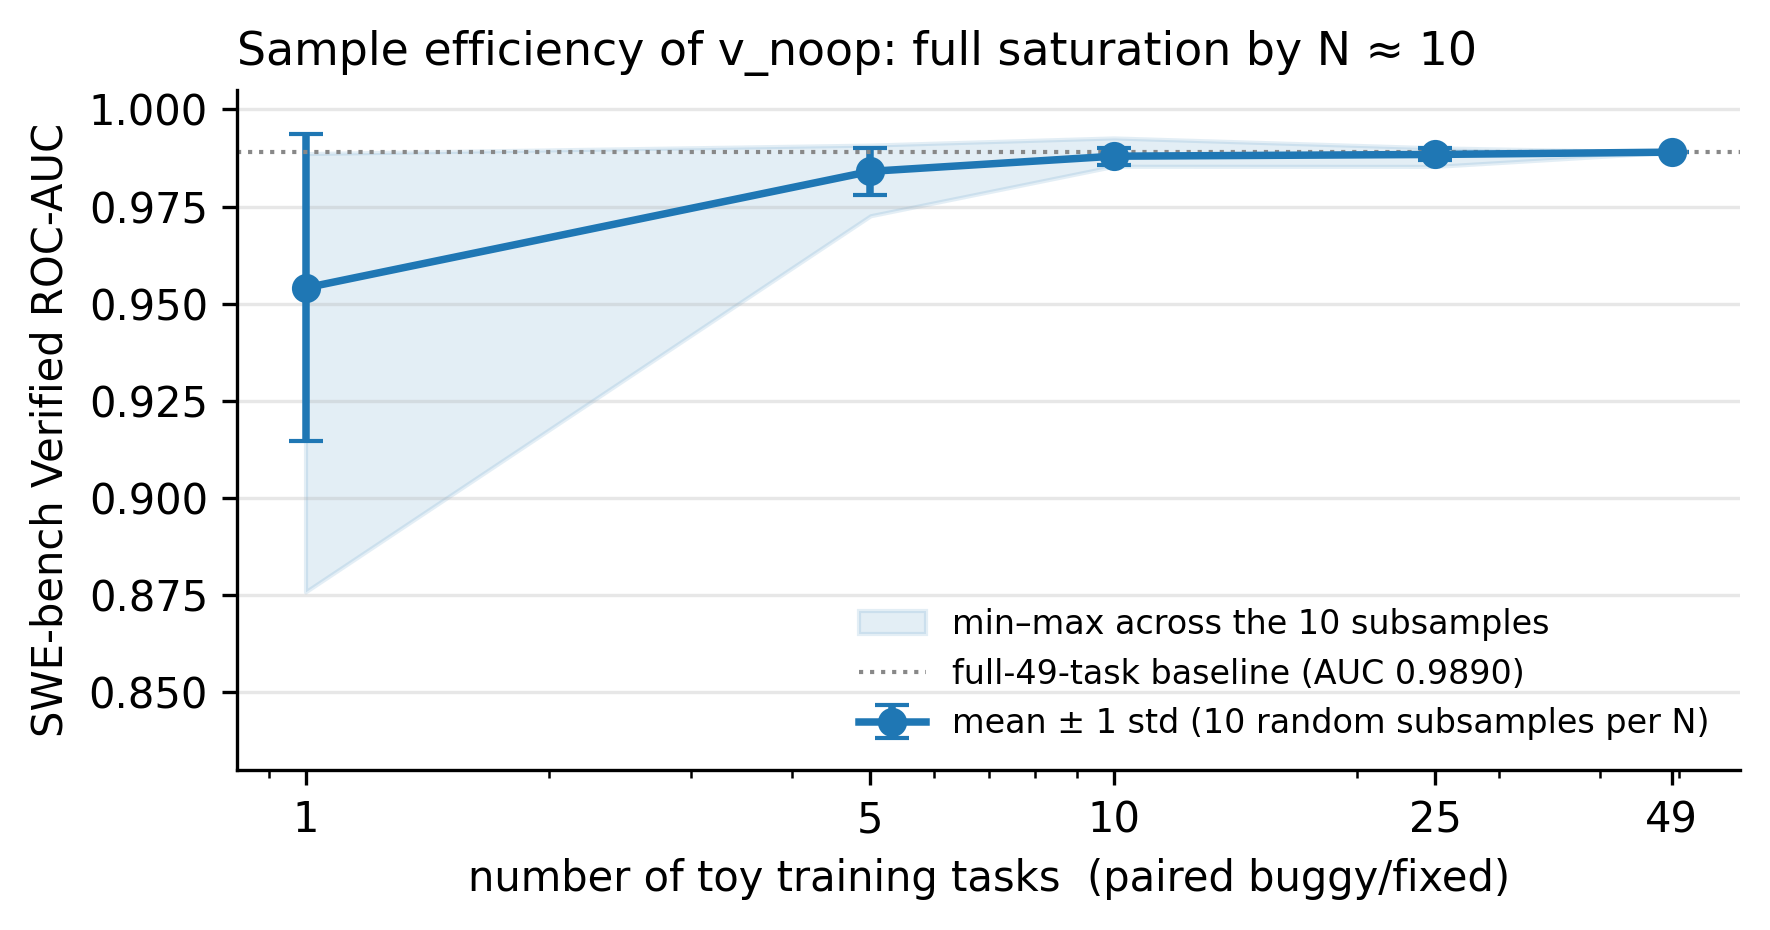
\includegraphics[width=0.85\linewidth,height=\textheight,keepaspectratio,alt={Sample-efficiency curve. AUC on the 499 SWE-bench-Verified-derived paired prompts (the same evaluation set used in \S{}5.1), as a function of the number of paired buggy/fixed toy tasks used to derive u\_\{\textbackslash rm tx\}. Mean \ensuremath{\pm} 1 std across 10 random subsamples per N; the N=49 full-set draw is deterministic. Saturation at N \ensuremath{\approx} 10 (mean AUC 0.988 vs full-set 0.989). The evaluation set is the same throughout, so this is implicit-model-selection-vulnerable; a held-out transcript-containing stale/no-edit benchmark or a transcript-observing agent-loop harness would give a stronger reading.}]{figures/sample_efficiency.png}
\caption{Sample-efficiency curve. AUC on the 499
SWE-bench-Verified-derived paired prompts (the same evaluation set used
in \S{}5.1), as a function of the number of paired buggy/fixed toy tasks
used to derive \(u_{\rm tx}\). Mean \ensuremath{\pm} 1 std across 10 random subsamples
per N; the N=49 full-set draw is deterministic. Saturation at N \ensuremath{\approx} 10
(mean AUC 0.988 vs full-set 0.989). The evaluation set is the same
throughout, so this is implicit-model-selection-vulnerable; a held-out
transcript-containing stale/no-edit benchmark or a transcript-observing
agent-loop harness would give a stronger
reading.}\label{fig:sample-efficiency}
\end{figure}

Two reads of this. (i) \textbf{Low label cost for monitor bootstrapping
under our prompt format:} \textasciitilde10 paired tasks suffice to
reach within 0.001 AUC of the full-49 baseline on this evaluation set.
(ii) The contrast direction is detectable in the residual stream after
even a single paired comparison (mean AUC 0.954 at N = 1), so the
direction is not solely an averaging artifact. The result is suggestive
of low-label-cost monitor bootstrapping but is not itself a
deployment-readiness claim; see \S{}6.1 for the controls a deployment claim
would require.

\textbf{Cross-model extension.} Re-running the same subsample sweep on
CodeGemma-7B (L26/pos \ensuremath{-}1, 497 SWE-derived prompts) and DeepSeek-
Coder-1.3B (L22/pos \ensuremath{-}1, 499 SWE-derived prompts) yields:

{\def\LTcaptype{none} % do not increment counter
\begin{longtable}[]{@{}lrrr@{}}
\toprule\noalign{}
N & Qwen mean AUC & CodeGemma mean AUC & DeepSeek mean AUC \\
\midrule\noalign{}
\endhead
\bottomrule\noalign{}
\endlastfoot
1 & 0.954 \ensuremath{\pm} 0.040 & 0.825 \ensuremath{\pm} 0.096 & 0.888 \ensuremath{\pm} 0.045 \\
5 & 0.984 \ensuremath{\pm} 0.006 & 0.935 \ensuremath{\pm} 0.024 & 0.897 \ensuremath{\pm} 0.025 \\
10 & 0.988 \ensuremath{\pm} 0.002 & 0.935 \ensuremath{\pm} 0.013 & 0.887 \ensuremath{\pm} 0.013 \\
25 & 0.988 \ensuremath{\pm} 0.002 & 0.947 \ensuremath{\pm} 0.009 & 0.887 \ensuremath{\pm} 0.006 \\
49 & \textbf{0.989} & \textbf{0.950} & \textbf{0.888} \\
\end{longtable}
}

The same low-label-cost pattern appears on all three models under this
evaluation protocol: mean AUC at N=5 is within \textasciitilde0.005,
0.015, and 0.000 of the full-49 baseline on Qwen / CodeGemma / DeepSeek
respectively. DeepSeek's N=1 mean matches the full-set AUC (0.888),
though individual one-pair draws vary substantially (std \ensuremath{\pm}0.045 at N=1),
consistent with the \S{}6 toy-vs-SWE-derived saliency-divergence
observation.

\textbf{CodeGemma headline uses all 49 toys.} The CodeGemma N=49 number
above (AUC \textbf{0.950}, AP 0.949, in-sample fixed-condition FPR
0.105) is the \S{}5.1 headline, computed from the all-49 direction; the
20-task responsive subset is retained only for \S{}4.2 steering and the
exploratory CodeGemma SAE in App. H.6 (rationale in \S{}5.1 and \S{}4.3).

\clearpage

\begin{figure}
\centering
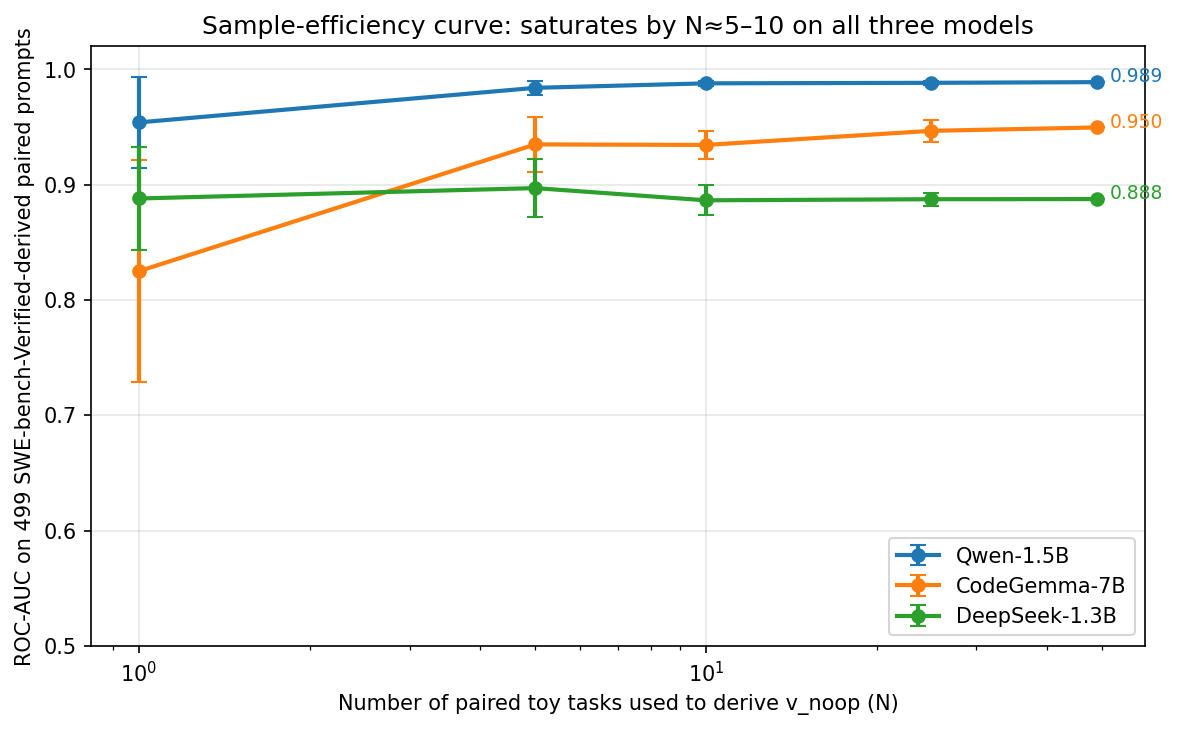
\includegraphics[width=0.85\linewidth,height=\textheight,keepaspectratio,alt={Cross-model sample-efficiency curves. AUC on each model's paired-prompt set (499/497/499 for Qwen/CodeGemma/DeepSeek) as a function of subsample size N, error bars are mean \ensuremath{\pm} std across 10 random subsamples. All three models saturate by N \ensuremath{\approx} 5--10. Compute: scripts/sample\_efficiency\_curve.py.}]{figures/sample_efficiency_cross_model.png}
\caption{Cross-model sample-efficiency curves. AUC on each model's
paired-prompt set (499/497/499 for Qwen/CodeGemma/DeepSeek) as a
function of subsample size N, error bars are mean \ensuremath{\pm} std across 10 random
subsamples. All three models saturate by N \ensuremath{\approx} 5--10. Compute:
\protect\texttt{scripts/sample\_efficiency\_curve.py}.}
\end{figure}

Outputs: \texttt{results/monitor\_real/sample\_efficiency.json} (Qwen),
\texttt{sample\_efficiency\_codegemma.json},
\texttt{sample\_efficiency\_deepseek.json}.

\subsection{Qwen held-out threshold
calibration}\label{qwen-held-out-threshold-calibration}

\textbf{This section reports Qwen-only threshold calibration; CodeGemma
and DeepSeek held-out calibration under the updated all-49 direction
remains future work.}

The \S{}5.1 operating-point precision/recall/fixed-condition-FPR values use
a balanced-accuracy threshold fit on the same model-specific evaluation
set (499/497/499 for Qwen/CodeGemma/DeepSeek), so they are
\emph{in-sample}. Two held-out designs (no new compute, just refitting
the threshold on different splits of the existing per-task scores;
\texttt{scripts/held\_out\_threshold\_calibration.py}):

{\def\LTcaptype{none} % do not increment counter
\begin{longtable}[]{@{}
  >{\raggedright\arraybackslash}p{(\linewidth - 6\tabcolsep) * \real{0.3700}}
  >{\raggedleft\arraybackslash}p{(\linewidth - 6\tabcolsep) * \real{0.2100}}
  >{\raggedleft\arraybackslash}p{(\linewidth - 6\tabcolsep) * \real{0.2100}}
  >{\raggedleft\arraybackslash}p{(\linewidth - 6\tabcolsep) * \real{0.2100}}@{}}
\toprule\noalign{}
\begin{minipage}[b]{\linewidth}\raggedright
design
\end{minipage} & \begin{minipage}[b]{\linewidth}\raggedleft
precision
\end{minipage} & \begin{minipage}[b]{\linewidth}\raggedleft
recall
\end{minipage} & \begin{minipage}[b]{\linewidth}\raggedleft
fixed-cond. FPR
\end{minipage} \\
\midrule\noalign{}
\endhead
\bottomrule\noalign{}
\endlastfoot
\textbf{in-sample (\S{}5.1, for reference)} & 0.973 & 0.938 & 0.026 \\
random 50/50 split, 200 seeds, mean & \textbf{0.964} & 0.938 &
\textbf{0.035} \\
random 50/50 split, {[}2.5\%, 97.5\%{]} & {[}0.931, 0.983{]} & {[}0.908,
0.972{]} & {[}0.016, 0.072{]} \\
leave-one-repo-out (12 repos), pooled & \textbf{0.967} & 0.938 &
\textbf{0.032} \\
\end{longtable}
}

The held-out precision drops modestly (0.973 \ensuremath{\rightarrow} 0.964--0.967), recall is
essentially unchanged (0.938 throughout), and the fixed-condition FPR
rises from 2.6\% \ensuremath{\rightarrow} 3.2--3.5\%. The \S{}5.1 numbers are slightly optimistic
but not catastrophically so; the monitor's \emph{threshold-free} AUC of
0.989 is unaffected by this analysis, and the held-out operating point
remains at \ensuremath{\approx} 96.5\% precision with \ensuremath{\approx} 94\% recall on the
SWE-bench-Verified-derived paired prompts. Per-repo LOO threshold
distribution (\texttt{results/monitor\_real/held\_out\_thresholds.json})
shows that 9 of 12 repos give precision \ensuremath{\geq} 0.95 on their held-out fold;
the outlier is \texttt{pylint\_dev} (precision 0.692, N\_fixed = 10),
consistent with the per-repo regression in App. G.3.

\subsection{Lexical-redaction controls (Qwen): literal tokens, redaction
artifacts, and structural
signal}\label{lexical-redaction-controls-qwen-literal-tokens-redaction-artifacts-and-structural-signal}

\S{}5.2 shows the \S{}5.1 monitor follows transcript text. A natural
follow-up: how much of that is the \emph{literal} \texttt{FAILED} /
\texttt{passed} tokens, vs a broader pass/fail representation that
survives lexical redaction? We run two levels of redaction.

\textbf{Level 1 (\texttt{code\_tests\_lex\_redacted}).} Per-token
mapping that preserves character count within 1--3:

{\def\LTcaptype{none} % do not increment counter
\begin{longtable}[]{@{}ll@{}}
\toprule\noalign{}
original & replacement \\
\midrule\noalign{}
\endhead
\bottomrule\noalign{}
\endlastfoot
\texttt{FAILURES} & \texttt{REDACTED} \\
\texttt{FAILED} & \texttt{REDACT} \\
\texttt{AssertionError} & \texttt{RedactedErr\_\_\_} \\
\texttt{passed} & \texttt{redact} \\
\texttt{failed} & \texttt{redact} \\
\texttt{Traceback} & \texttt{Trace\_\_\_\_\_\_\_\_} \\
\texttt{OK\textbackslash{}n} & \texttt{\_\_\_\textbackslash{}n} \\
\end{longtable}
}

This redaction still leaks class information: buggy transcripts get
UPPERCASE replacements (\texttt{REDACT}, \texttt{REDACTED},
\texttt{RedactedErr\_\_\_}) while fixed transcripts get the lowercase
\texttt{redact}. Case and substring shape differ between classes.

\textbf{Level 2 (\texttt{code\_tests\_lex\_redacted\_uniform}).}
Stricter: all pass/fail vocabulary maps to a single case-uniform token
\texttt{OUTCOME}. After this both buggy and fixed transcripts contain
literally \texttt{OUTCOME} tokens; only their \emph{counts} and the
surrounding structural shape (failure-section length, summary line)
differ between classes.

We re-cache 499 paired SWE-bench-Verified-derived prompts on Qwen-1.5B
and score with the frozen toy-trained unit monitor direction
\(u_{\rm tx}\) (gap = mean-fixed \ensuremath{-} mean-buggy projection \(p\)):

{\def\LTcaptype{none} % do not increment counter
\begin{longtable}[]{@{}lrr@{}}
\toprule\noalign{}
variant & ROC-AUC & mean gap \\
\midrule\noalign{}
\endhead
\bottomrule\noalign{}
\endlastfoot
\texttt{code\_tests} (\S{}5.1) & \textbf{0.989} & +4.73 \\
\texttt{code\_tests\_lex\_redacted} (Level 1) & 0.865 & +2.05 \\
\texttt{code\_tests\_lex\_redacted\_uniform} (Level 2) & \textbf{0.905}
& +2.55 \\
\end{longtable}
}

The uniform redaction (Level 2) actually gives a \emph{slightly higher}
AUC than the per-token redaction (Level 1), 0.905 vs 0.865, so the Level
1 case/substring artifacts were not, in fact, doing the work. Both
redactions converge on the same picture: stripping the explicit
pass/fail vocabulary costs the projection \textasciitilde8--12 AUC
points, but the residual stays well above chance. The direction is
partly literal-token-driven and partly structural (line count, presence
of failure listing, summary-line shape). We cannot, from these controls
alone, distinguish ``the projection is responding to an abstract
pass/fail signal'' from ``the projection is responding to the structural
shape of pass/fail transcripts.'' Appendix G.12 adds a deterministic
paraphrase control, but stronger length-matched and held-out paraphrase
controls would be needed to disambiguate semantic readout from
format-specific lexical/structural cues.

Outputs: \texttt{results/monitor\_real/lex\_redact\_scores.json},
\texttt{results/monitor\_real/lex\_redact\_uniform\_scores.json}.

\subsection{Action-vocabulary swap (Qwen): 0\% explicit-noop is not a
noop-token
artifact}\label{action-vocabulary-swap-qwen-0-explicit-noop-is-not-a-noop-token-artifact}

The 0\% explicit-\texttt{noop} rate (\S{}5) could in principle be an
artifact of the literal token \texttt{noop} rather than a fact about the
model's abstention prior. We re-cache the 499 paired prompts on
Qwen-1.5B with the action vocabulary replaced (\texttt{view},
\texttt{grep}, \texttt{test}, \texttt{edit}, \emph{synonym}) for two
synonyms, and read off both the projection AUC (transfer of
\(u_{\rm tx}\)) and the synonym argmax rate.

{\def\LTcaptype{none} % do not increment counter
\begin{longtable}[]{@{}
  >{\raggedright\arraybackslash}p{(\linewidth - 6\tabcolsep) * \real{0.5200}}
  >{\raggedleft\arraybackslash}p{(\linewidth - 6\tabcolsep) * \real{0.0900}}
  >{\raggedleft\arraybackslash}p{(\linewidth - 6\tabcolsep) * \real{0.0700}}
  >{\raggedright\arraybackslash}p{(\linewidth - 6\tabcolsep) * \real{0.3200}}@{}}
\toprule\noalign{}
\begin{minipage}[b]{\linewidth}\raggedright
action vocabulary
\end{minipage} & \begin{minipage}[b]{\linewidth}\raggedleft
ROC-AUC
\end{minipage} & \begin{minipage}[b]{\linewidth}\raggedleft
projection gap
\end{minipage} & \begin{minipage}[b]{\linewidth}\raggedright
synonym argmax (buggy / fixed)
\end{minipage} \\
\midrule\noalign{}
\endhead
\bottomrule\noalign{}
\endlastfoot
\texttt{view,\ grep,\ test,\ edit,\ noop} (\S{}5.1, reference) & 0.989 &
+4.73 & 0.0\% / 0.0\% \\
\texttt{view,\ grep,\ test,\ edit,\ done} & \textbf{0.990} & +4.65 &
\textbf{0.0\% / 0.0\%} \\
\texttt{view,\ grep,\ test,\ edit,\ skip} & \textbf{0.988} & +4.55 &
\textbf{0.0\% / 0.0\%} \\
\end{longtable}
}

Two findings. (i) \textbf{\(u_{\rm tx}\) transfers cleanly across action
vocabularies.} AUC and projection gap are essentially unchanged when the
abstention token is swapped, consistent with the residual at the action
position being computed before any action token is generated. (ii)
\textbf{The 0\% explicit-abstention rate is not an artifact of the
literal \texttt{noop} token.} Replacing \texttt{noop} with \texttt{done}
or \texttt{skip} keeps the abstention argmax at 0\% on both buggy and
fixed conditions across all 499 paired prompts; the model defaults to
\texttt{grep} \textgreater93\% of the time under both alternative
vocabularies, with \texttt{edit} taking the rest. These swaps rule out
the narrow \emph{content-prior} reading that the literal token
\texttt{noop} is uniquely avoided. The broader \emph{position-prior}
explanation is addressed by the position-balanced, binary, and
abstract-label controls in \S{}5.5: on Qwen and CodeGemma abstention stays
near-zero at every named-menu position, while a single-token DeepSeek
rerun instead shows a first-position bias.

Outputs: \texttt{results/monitor\_real/vocab\_done\_scores.json},
\texttt{results/monitor\_real/vocab\_skip\_scores.json}.

\subsection{The obvious baseline: a regex over the transcript
text}\label{the-obvious-baseline-a-regex-over-the-transcript-text}

Given \S{}5.2's finding that the projection monitor is reading transcript
text, the natural baseline is a regex or pytest-summary parser. We
compute three trivial classifiers over the synthesized transcripts
(\texttt{scripts/regex\_transcript\_baseline.py}):

{\def\LTcaptype{none} % do not increment counter
\begin{longtable}[]{@{}
  >{\raggedright\arraybackslash}p{(\linewidth - 10\tabcolsep) * \real{0.4000}}
  >{\raggedleft\arraybackslash}p{(\linewidth - 10\tabcolsep) * \real{0.1125}}
  >{\raggedleft\arraybackslash}p{(\linewidth - 10\tabcolsep) * \real{0.1000}}
  >{\raggedleft\arraybackslash}p{(\linewidth - 10\tabcolsep) * \real{0.1375}}
  >{\raggedleft\arraybackslash}p{(\linewidth - 10\tabcolsep) * \real{0.1000}}
  >{\raggedleft\arraybackslash}p{(\linewidth - 10\tabcolsep) * \real{0.1500}}@{}}
\toprule\noalign{}
\begin{minipage}[b]{\linewidth}\raggedright
classifier
\end{minipage} & \begin{minipage}[b]{\linewidth}\raggedleft
ROC-AUC
\end{minipage} & \begin{minipage}[b]{\linewidth}\raggedleft
AP
\end{minipage} & \begin{minipage}[b]{\linewidth}\raggedleft
precision
\end{minipage} & \begin{minipage}[b]{\linewidth}\raggedleft
recall
\end{minipage} & \begin{minipage}[b]{\linewidth}\raggedleft
fixed-cond. FPR
\end{minipage} \\
\midrule\noalign{}
\endhead
\bottomrule\noalign{}
\endlastfoot
\texttt{contains("FAILED")} & \textbf{1.000} & 1.000 & 1.000 & 1.000 &
0.000 \\
count of \texttt{FAILED} lines & \textbf{1.000} & 1.000 & 1.000 & 1.000
& 0.000 \\
failure-line density & \textbf{1.000} & 1.000 & 1.000 & 1.000 & 0.000 \\
\end{longtable}
}

All three are perfect on each model's paired-prompt set (499/497/499)
because the synthesized buggy and fixed transcripts differ
deterministically (buggy contains FAILED lines, fixed does not). The
projection monitor's \S{}5.1 AUC of 0.989/0.950/0.888 is \textbf{strictly
worse} than this baseline.

\textbf{Implication.} The value of the residual-projection monitor
relative to a trivial transcript parser is not discriminative power. It
is mechanistic: it identifies the residual-stream location and direction
at which pass/fail evidence is read out into the action-token
computation and shows that this evidence \emph{causally} affects the
\texttt{edit\ \ensuremath{-}\ noop} margin (\S{}4.1, \S{}4.2). If an external system has
the pytest transcript, it should parse the transcript. The projection
monitor is interesting only if one of the following holds: (a) the model
sees evidence the external system cannot parse, (b) the transcript is
paraphrased or noisy, or (c) the monitor is needed at an internal
decision point where transcript evidence is temporally separated from
the current text (e.g.~multi-turn agent traces). As App. G.15 shows,
case (c) only beats a stateless turn-local parser; a full-history regex
or stateful parser still recovers the upstream transcript. App. G.9
reports the code-only no-transcript evaluation, decisively negative for
the Qwen L24 linear monitor.

Output: \texttt{results/monitor\_real/regex\_transcript\_baseline.json}.

\subsection{No-transcript SWE-derived evaluation (Qwen): bounding the
L24-monitor
approach}\label{no-transcript-swe-derived-evaluation-qwen-bounding-the-l24-monitor-approach}

The single most important deployment-relevance question after \S{}5.2 was:
does the residual direction generalize to settings \emph{without} a
transcript? If yes, the paper has a no-transcript stale-bug deployment
niche (FixedBench-style; \citet{fixedbench2025}). If no, the mechanism
is bound to the transcript pathway and the paper is a mechanistic case
study.

\textbf{Design.} We re-cache the 499 paired SWE-bench-Verified-derived
tasks on Qwen-1.5B under the existing \texttt{code} variant (issue text
+ code, \emph{no} pytest transcript;
\texttt{src/no\_op\_circuit/dataset/schema.py}). Both buggy and fixed
conditions share the same prompt format, differing only in the code
itself. At Qwen L24/pos \ensuremath{-}1 we then run three increasingly-strong tests
on the resulting 998 residuals
(\texttt{scripts/no\_transcript\_full\_analysis.py}):

{\def\LTcaptype{none} % do not increment counter
\begin{longtable}[]{@{}
  >{\raggedright\arraybackslash}p{(\linewidth - 4\tabcolsep) * \real{0.0423}}
  >{\raggedright\arraybackslash}p{(\linewidth - 4\tabcolsep) * \real{0.7606}}
  >{\raggedleft\arraybackslash}p{(\linewidth - 4\tabcolsep) * \real{0.1972}}@{}}
\toprule\noalign{}
\begin{minipage}[b]{\linewidth}\raggedright
\#
\end{minipage} & \begin{minipage}[b]{\linewidth}\raggedright
classifier
\end{minipage} & \begin{minipage}[b]{\linewidth}\raggedleft
ROC-AUC
\end{minipage} \\
\midrule\noalign{}
\endhead
\bottomrule\noalign{}
\endlastfoot
1 & \textbf{Frozen toy-trained \(u_{\rm tx}\)} (\S{}5.1 transfer) &
\textbf{0.4987} \\
2 & Fresh
\texttt{v\_no\_tx\ =\ mean(fixed\_code)\ \ensuremath{-}\ mean(buggy\_code)},
in-sample & 0.5432 \\
2' & Same direction, paired LOO out-of-sample & 0.5213 \\
3 & 1536-D LR probe at the same site, paired LOO & 0.5184 \\
\end{longtable}
}

The fresh direction has \(\| v_{\text{no\_tx}} \|\) = 0.156 (vs the
transcript-trained \(\|v_{\rm raw}\|\) = 5.89) and cosine \textbf{\ensuremath{-}0.04}
with the frozen direction, \emph{orthogonal}. The in-sample 0.543 is an
upper bound (the direction is fit on the same data it's evaluated on);
the paired-LOO out-of-sample drops to 0.521, and the LR probe gives
0.518. \textbf{None of the tested linear readouts at L24/pos \ensuremath{-}1
discriminates buggy from fixed code in the absence of a transcript}
(frozen \(u_{\rm tx}\), a fresh mean-difference direction, and a 1536-D
LR probe are all near chance).

The argmax distribution under no-transcript also matches the
``information-free'' expectation: 80\% \texttt{grep}, 20\%
\texttt{edit}, \textasciitilde0\% \texttt{view} / \texttt{test} /
\texttt{noop} on \emph{both} conditions (the model can't tell buggy from
fixed apart and defaults to a \texttt{grep}-then-\texttt{edit} hedge
regardless).

\textbf{What this settles, narrowly.} Combined with \S{}5.2 (contradictory-
transcript flips the score) and \S{}C / App. D (toy \texttt{code} variant
has no patching peak), this establishes that:

\begin{itemize}
\tightlist
\item
  The mechanism this paper studies, \emph{a linear residual direction at
  L24/pos \ensuremath{-}1 on Qwen}, is bound to the pass/fail-test-transcript
  pathway. There is no separate ``no-edit decision'' representation at
  this site readable along this direction.
\item
  For this L24/pos \ensuremath{-}1 linear-residual-monitor approach, a no-transcript
  deployment is \textbf{not supported} by our data, we find no usable
  signal for the tested L24/pos \ensuremath{-}1 linear readouts to project onto. We
  do \textbf{not} claim this rules out \emph{all} no-transcript
  detection: a different layer or position, a nonlinear probe, a full
  agent trace, or a semantic code embedding might do better. We also
  note this is not an actual FixedBench evaluation, only a no-transcript
  SWE-bench-derived ablation; we use the phrase
  ``FixedBench-\emph{style}'' advisedly.
\item
  The paper is a mechanistic case study of how a transcript-evidence
  representation at the action-token residual-stream site affects the
  action decision, \textbf{not} a stale-bug deployment paper.
\end{itemize}

Output:
\texttt{results/monitor\_real/no\_transcript\_full\_analysis.json};
cache:
\texttt{results/}\allowbreak\texttt{cache-real-qwen-code-only-}\allowbreak\texttt{20260518T092253Z/}.

\subsection{Single-turn edit-action veto simulation: projection vs regex
gate}\label{single-turn-edit-action-veto-simulation-projection-vs-regex-gate}

\S{}G.8's regex baseline classifies each model-specific paired-prompt set
(499/497/499 for Qwen/CodeGemma/DeepSeek) at AUC 1.000, so as a
classifier the projection is dominated. The remaining defensible
question is \textbf{as an edit-action gate}: when the model's
first-token argmax is \texttt{edit}, can the projection veto
fixed-condition (spurious) edits without killing too many
buggy-condition (useful) ones? We report this in the obvious six-bucket
form, alongside the same gate evaluation for the regex baseline so the
comparison is apples-to-apples.

\textbf{Important framing note.} This is \textbf{not} a multi-step agent
loop. The ``agent'' here emits a single first-token action; if it is
\texttt{edit}, the gate decides whether to allow or veto. A real
SWE-agent / OpenHands / Aider harness lets the agent \texttt{grep},
\texttt{view}, run tools, iterate, and emit an actual patch, none of
which we simulate. This is a single-turn edit-action veto simulation,
not a multi-step agent-loop evaluation.

\textbf{Setup.} For each model's paired prompts (499/497/499 buggy +
499/497/499 fixed for Qwen / CodeGemma / DeepSeek), we record the
first-token argmax and apply two candidate gates:

\begin{itemize}
\tightlist
\item
  \textbf{Residual projection gate.} Project
  \texttt{resid\_pre{[}L\_site,\ pos\ \ensuremath{-}1{]}} onto each model's frozen
  unit monitor direction \(u_{\rm tx}\) (legacy \texttt{v\_noop}) to get
  the classifier score \(s=-h\cdot u_{\rm tx}\), where higher means
  failing-transcript/edit-warranted evidence. The gate vetoes an
  \texttt{edit} action when \(s\) is below the model-specific threshold.
  Thresholds are model-specific: Qwen uses the App. G.5 held-out 50/50
  mean threshold; DeepSeek uses a computed held-out 50/50 mean threshold
  stored in \texttt{results/monitor\_real/agent\_loop\_simulation.json};
  CodeGemma uses the \S{}5.1 in-sample balanced-accuracy threshold under
  the all-49 direction. Formal held-out re-calibration for the all-49
  CodeGemma direction remains future work.
\item
  \textbf{Regex gate.} Allow the edit iff the prompt's pytest transcript
  contains the literal token \texttt{FAILED}.
\end{itemize}

Each prompt falls into one of six outcome buckets (A--F):

A. useful edit committed (buggy, argmax=edit, ALLOW) B. useful edit not
proposed (buggy, argmax!=edit) C. useful edit VETOED (buggy,
argmax=edit, VETO) (bad) D. SPURIOUS edit committed (fixed, argmax=edit,
ALLOW) (bad) E. spurious not proposed (fixed, argmax!=edit) F. SPURIOUS
edit BLOCKED (fixed, argmax=edit, VETO) (good)

spurious-edit reduction = F / (D + F) useful-edit loss = C / (A + C)

\textbf{Results.} Both gates evaluated on each model's paired-prompt set
(499/497/499 for Qwen/CodeGemma/DeepSeek):

{\def\LTcaptype{none} % do not increment counter
\begin{longtable}[]{@{}
  >{\raggedright\arraybackslash}p{(\linewidth - 8\tabcolsep) * \real{0.1835}}
  >{\raggedright\arraybackslash}p{(\linewidth - 8\tabcolsep) * \real{0.1651}}
  >{\raggedleft\arraybackslash}p{(\linewidth - 8\tabcolsep) * \real{0.2294}}
  >{\raggedleft\arraybackslash}p{(\linewidth - 8\tabcolsep) * \real{0.1651}}
  >{\raggedleft\arraybackslash}p{(\linewidth - 8\tabcolsep) * \real{0.2569}}@{}}
\toprule\noalign{}
\begin{minipage}[b]{\linewidth}\raggedright
model
\end{minipage} & \begin{minipage}[b]{\linewidth}\raggedright
gate
\end{minipage} & \begin{minipage}[b]{\linewidth}\raggedleft
spurious-edit reduction
\end{minipage} & \begin{minipage}[b]{\linewidth}\raggedleft
useful-edit loss
\end{minipage} & \begin{minipage}[b]{\linewidth}\raggedleft
final spurious-action rate
\end{minipage} \\
\midrule\noalign{}
\endhead
\bottomrule\noalign{}
\endlastfoot
Qwen-1.5B & residual projection & 100.0\% (85/85) & 29.2\% (14/48) &
0.00\% (0/499) \\
Qwen-1.5B & \textbf{regex over transcript} & \textbf{100.0\%} (85/85) &
\textbf{0.0\%} (0/48) & \textbf{0.00\%} (0/499) \\
CodeGemma-7B & residual projection & 89.4\% (439/491) & 11.9\% (59/496)
& 10.46\% (52/497) \\
CodeGemma-7B & \textbf{regex over transcript} & \textbf{100.0\%}
(491/491) & \textbf{0.0\%} (0/496) & \textbf{0.00\%} (0/497) \\
DeepSeek-1.3B & residual projection & 84.4\% (65/77) & 23.9\% (26/109) &
2.40\% (12/499) \\
DeepSeek-1.3B & \textbf{regex over transcript} & \textbf{100.0\%}
(77/77) & \textbf{0.0\%} (0/109) & \textbf{0.00\%} (0/499) \\
\end{longtable}
}

(Thresholds are the model-specific ones defined in the Setup above. The
CodeGemma row uses the all-49 direction, which gives better gate metrics
than the responsive-subset direction used only for the steering plot,
spurious-edit reduction 89.4\% vs 84.7\%, final spurious-action rate
10.46\% vs 15.09\%, at unchanged useful-edit loss.)

\textbf{Reading.} In this clean synthesized-transcript setting, the
regex gate \textbf{strictly dominates} the residual projection on every
model: 100\% spurious-edit reduction at 0\% useful-edit loss. This is
unsurprising, the buggy and fixed transcripts differ deterministically
in containing \texttt{FAILED}, so a single-token check is sufficient for
the gate problem. The residual projection is therefore \textbf{not}
proposed as a deployment-superior gate in this setting. What \S{}G.10 does
show is that the residual signal is \emph{aligned with} the right gate
decisions, it correctly identifies most fixed-condition first-token edit
actions and blocks them, but it is mechanistically informative, not
operationally superior to direct transcript parsing.

Settings where a residual gate would need separate evaluation (none
validated here) include: (i) transcripts paraphrased into natural
language; (ii) transcript-text ambiguous (mixed pass/fail, flaky tests);
(iii) settings without \texttt{FAILED}-like keywords at all. On temporal
separation specifically: a constructed single-pass temporal-separation
setting is evaluated in App. G.15, the residual beats a stateless
turn-local regex but not a full-history regex or stateful parser. What
remains unvalidated is a live multi-step agent loop with
retry-after-veto dynamics, KV-cache continuation, and possible context
eviction. The code-only absent-transcript setting is \textbf{decisively
negative} for this L24 linear monitor (App. G.9) and is \textbf{not} in
the future-niche list above.

\textbf{Limitations of this simulation,} beyond the regex dominance
above:

\begin{itemize}
\tightlist
\item
  \textbf{Single-turn.} A real multi-step agent that can \texttt{grep}
  after a veto and re-decide might pay smaller useful-edit costs; this
  remains future work.
\item
  \textbf{First-token argmax, not patch generation.} The ``agent'' here
  produces a single action token; a real agent commits a multi-file
  patch with validation; ``spurious edit'' here means
  \textbf{fixed-condition first-token edit actions}, not committed PRs.
\item
  \textbf{No retry / iteration cost modeled.} A veto in a real loop
  forces another action; that cost is not measured.
\end{itemize}

Outputs: \texttt{results/monitor\_real/agent\_loop\_simulation.json}
(residual gate; full per-(model, threshold) bucket counts);
\texttt{results/monitor\_real/regex\_gate\_simulation.json} (regex
gate); \texttt{scripts/agent\_loop\_monitor\_simulation.py},
\texttt{scripts/regex\_gate\_baseline.py}.

\subsection{Robustness analyses: threshold sweep, per-repo, case study,
layer
sweep}\label{robustness-analyses-threshold-sweep-per-repo-case-study-layer-sweep}

Four post-hoc analyses on the existing cached scores (no new compute)
that bound the \S{}G.10 gate claims and the ``broadly distributed signal''
claim of \S{}G.2.

\textbf{(a) Threshold-sweep Pareto frontier.} \S{}G.10 reported two
operating points. The full sweep gives the gate trade-off curve; the
``knee'' (max of spurious reduction \ensuremath{-} useful loss):

{\def\LTcaptype{none} % do not increment counter
\begin{longtable}[]{@{}
  >{\raggedright\arraybackslash}p{(\linewidth - 8\tabcolsep) * \real{0.1688}}
  >{\raggedleft\arraybackslash}p{(\linewidth - 8\tabcolsep) * \real{0.1299}}
  >{\raggedleft\arraybackslash}p{(\linewidth - 8\tabcolsep) * \real{0.2597}}
  >{\raggedleft\arraybackslash}p{(\linewidth - 8\tabcolsep) * \real{0.2338}}
  >{\raggedleft\arraybackslash}p{(\linewidth - 8\tabcolsep) * \real{0.2078}}@{}}
\toprule\noalign{}
\begin{minipage}[b]{\linewidth}\raggedright
model
\end{minipage} & \begin{minipage}[b]{\linewidth}\raggedleft
knee thr
\end{minipage} & \begin{minipage}[b]{\linewidth}\raggedleft
spurious reduction
\end{minipage} & \begin{minipage}[b]{\linewidth}\raggedleft
useful-edit loss
\end{minipage} & \begin{minipage}[b]{\linewidth}\raggedleft
final spurious
\end{minipage} \\
\midrule\noalign{}
\endhead
\bottomrule\noalign{}
\endlastfoot
Qwen & \ensuremath{-}0.878 & \textbf{95.3\%} & \textbf{14.6\%} & 0.80\% \\
CodeGemma & \ensuremath{-}7.047 & 89.4\% & 11.7\% & 10.46\% \\
DeepSeek & \ensuremath{-}18.265 & 74.0\% & 8.3\% & 4.01\% \\
\end{longtable}
}

For Qwen, the knee threshold trades 5pp of spurious reduction (95\% vs
100\%) for 14.6pp of useful-edit recovery (15\% vs 29\% at held-out),
materially better than the balanced-accuracy default in many plausible
cost settings. CodeGemma's sweep is flat: the knee threshold is
essentially the in-sample balanced threshold (\ensuremath{-}7.047 vs \ensuremath{-}7.054), so the
\S{}G.10 operating point is already near-optimal. (CodeGemma row uses the
all-49 \texttt{v\_noop\_cg} direction; the 20-task responsive-subset
direction gives knee values 85.7\% / 12.5\% / 14.08\%.)

\begin{figure}
\centering
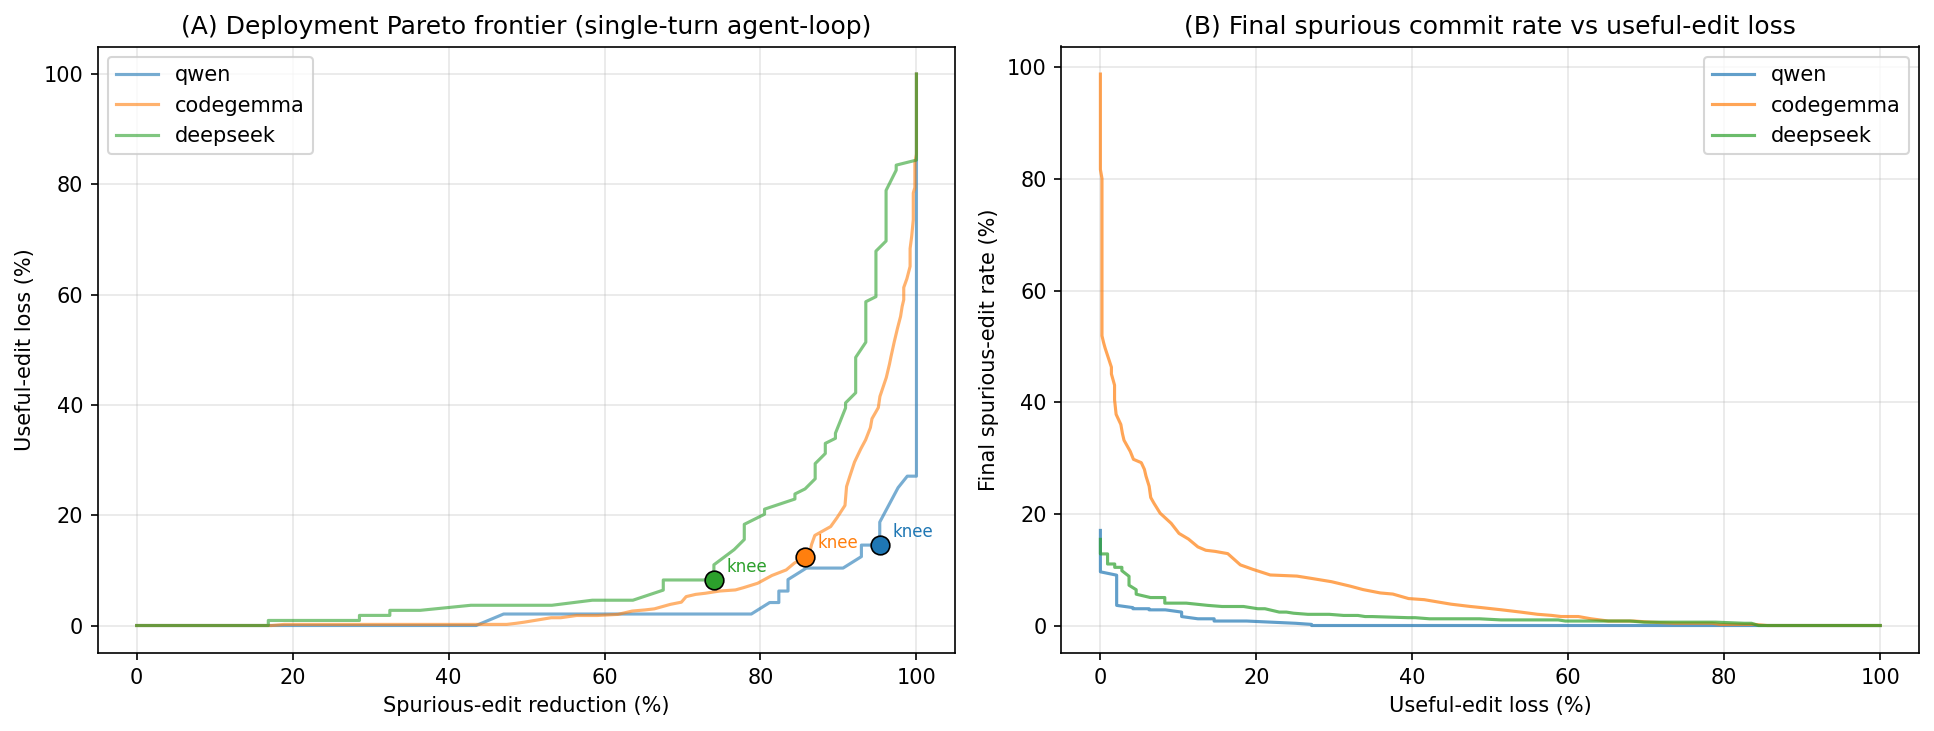
\includegraphics[width=0.98\linewidth,height=\textheight,keepaspectratio,alt={Threshold-sweep gate trade-off curves. (A) Pareto frontier: spurious-edit reduction vs useful-edit loss across the score range, with knee points (filled circles). (B) Final spurious-edit rate vs useful-edit loss. Source: scripts/threshold\_sweep\_deployment\_curve.py.}]{figures/threshold_sweep_deployment.png}
\caption{Threshold-sweep gate trade-off curves. \emph{(A)} Pareto
frontier: spurious-edit reduction vs useful-edit loss across the score
range, with knee points (filled circles). \emph{(B)} Final spurious-edit
rate vs useful-edit loss. Source:
\protect\texttt{scripts/threshold\_sweep\_deployment\_curve.py}.}
\end{figure}

\textbf{(b) Per-repo breakdown.} Across the 12 SWE-bench-Verified repos
at the held-out threshold (Qwen/DeepSeek) or in-sample balanced
threshold (CodeGemma, recomputed with all-49 \texttt{v\_noop\_cg}):
\textbf{Qwen} achieves 100\% spurious-edit reduction in every repo where
any spurious edits are proposed (final spurious rate 0/499 pooled);
useful-edit loss varies repo-to-repo (50\% sympy, 44\% scikit-learn, 0\%
several others). \textbf{CodeGemma}'s reduction now varies
\textbf{60--100\%} across repos with N\ensuremath{\geq}5, with
\texttt{pylint-dev/pylint} the outlier (60\% reduction at 40\% final
spurious rate on N = 10; same outlier the \S{}G.3 per-repo regression
flagged); \texttt{sphinx-doc/sphinx} sits next at 77\% / 23\%.
\textbf{DeepSeek}'s small-N repos show high-variance loss; large repos
(django, scikit-learn) sit at 80--100\% reduction.

\begin{figure}
\centering
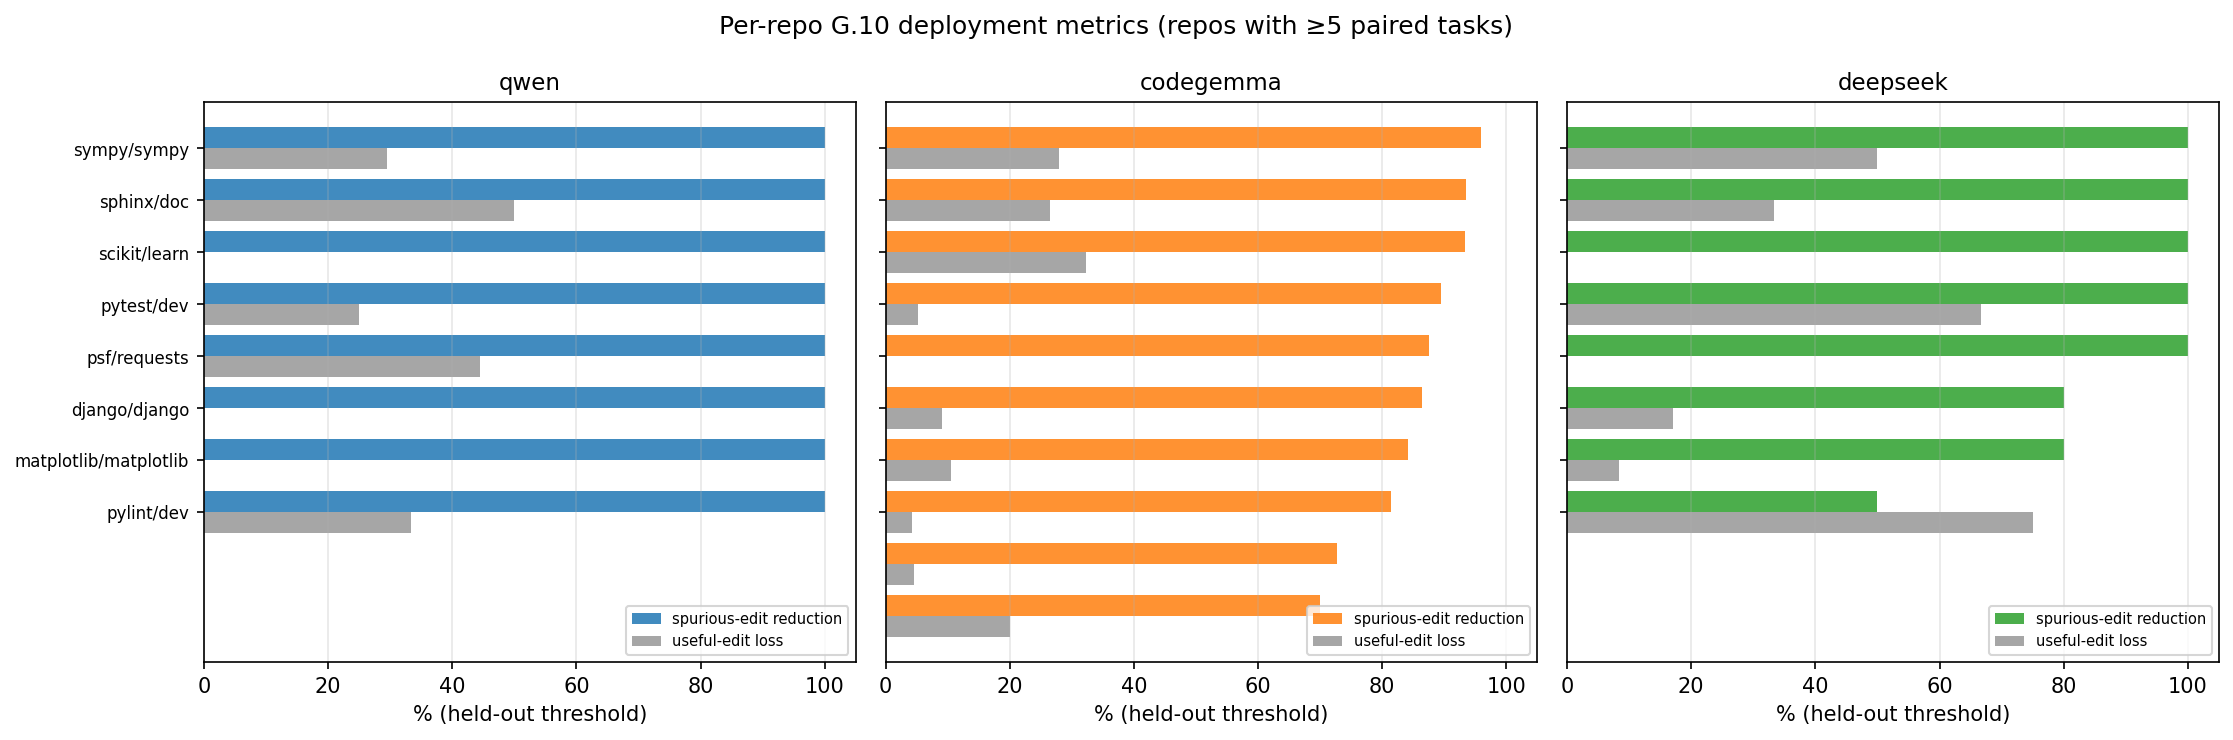
\includegraphics[width=0.99\linewidth,height=\textheight,keepaspectratio,alt={Per-repo G.10 metrics for the three models, repos with \ensuremath{\geq}5 paired tasks. Colored bars: spurious-edit reduction. Gray bars: useful-edit loss. Source: scripts/agent\_loop\_per\_repo\_and\_casestudy.py.}]{figures/per_repo_g10.png}
\caption{Per-repo G.10 metrics for the three models, repos with \ensuremath{\geq}5
paired tasks. Colored bars: spurious-edit reduction. Gray bars:
useful-edit loss. Source:
\protect\texttt{scripts/agent\_loop\_per\_repo\_and\_casestudy.py}.}
\end{figure}

\textbf{(c) Qwen over-veto case study.} The 14 Qwen Bucket-C cases
(useful edit proposed, monitor vetoed) reveal a clean failure pattern:
\textbf{13 of 14 buggy transcripts contain exactly 2 FAILED lines and 5
total lines}; the remaining one has 4 FAILED lines and 7 total lines.
All 14 are also vetoed at the held-out threshold. The pattern is
mechanistically consistent with App. G.6's structural-signal finding,
SWE-bench tasks with only 2 failing tests produce the shortest buggy
transcripts and sit at the failure-end of the monitor's veto envelope. A
practical mitigation for a future in-loop evaluation would be to fall
back to the regex baseline (App. G.8) when the transcript has fewer than
\textasciitilde3 FAILED lines.

\textbf{(d) Layer-sweep AUC.} App. G.2 reported one wrong-layer cell
(L12, AUC 0.998); the full 28-layer curve at pos \ensuremath{-}1 generalizes that
finding. These curves are descriptive on the same SWE-derived evaluation
set used elsewhere, not held-out model-selection evidence: each fresh
\texttt{v\_noop\_L} is fit on the 49 toy paired tasks at layer L and
then evaluated on the 499 SWE-derived prompts, while the frozen L24
direction is projected at different layers. The purpose is to show where
the signal is separable in residual space, not to claim held-out
generalization:

{\def\LTcaptype{none} % do not increment counter
\begin{longtable}[]{@{}crr@{}}
\toprule\noalign{}
layer & fresh \texttt{v\_noop\_L} AUC & frozen L24 AUC \\
\midrule\noalign{}
\endhead
\bottomrule\noalign{}
\endlastfoot
0 & 0.500 & 0.500 \\
5 & 0.999 & 0.732 \\
15 & 0.993 & 0.982 \\
20 & \textbf{1.000} & 1.000 \\
24 & 0.989 & 0.989 \\
27 & 0.985 & 0.983 \\
\end{longtable}
}

A fresh per-layer contrastive direction reaches AUC \ensuremath{\geq} 0.99 from L5
onwards and peaks at \textbf{L20}, not L24. The frozen L24-direction
transfers cleanly from L15+ and is inverted at very-early layers
(e.g.~L3 AUC 0.27, expected, early-layer residuals are
token-feature-dominated). Implication: the \S{}4.1 causal patching peak at
L24 is a causal \emph{readout} site for the \texttt{edit\ \ensuremath{-}\ noop}
submargin under intervention, not where the pass/fail signal is most
separable, separability and causal usage are distinct questions, and the
discriminative peak (L20) is upstream of the causal site by 4 layers.

\begin{figure}
\centering
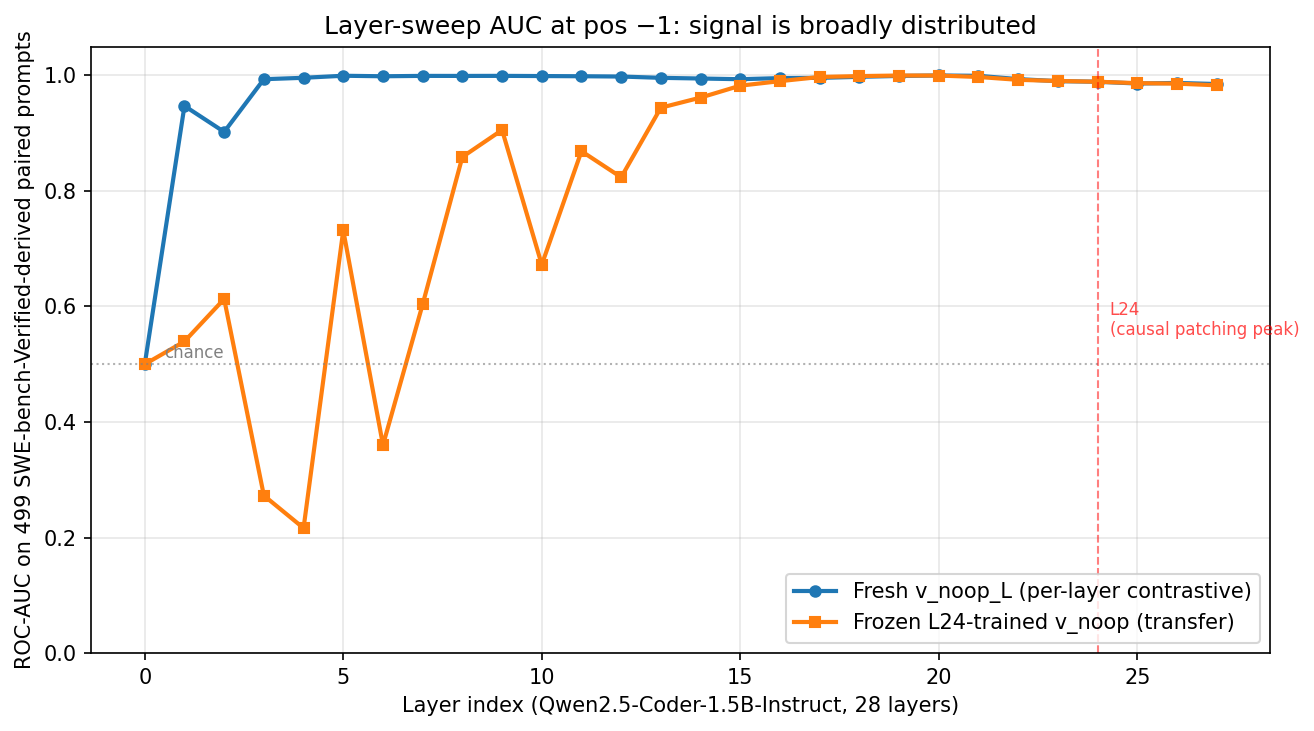
\includegraphics[width=0.92\linewidth,height=\textheight,keepaspectratio,alt={Layer-sweep AUC at pos \ensuremath{-}1 on Qwen (28 layers, 499 paired prompts). Fresh v\_noop\_L (per-layer contrastive direction, fit on the 49 toy tasks at layer L) vs frozen L24-trained v\_noop projected at each layer. Red dashed line marks L24. Both curves are descriptive on the same SWE-derived evaluation set used elsewhere (not held-out model selection). Source: scripts/layer\_sweep\_auc.py.}]{figures/layer_sweep_auc.png}
\caption{Layer-sweep AUC at pos \ensuremath{-}1 on Qwen (28 layers, 499 paired
prompts). Fresh \protect\texttt{v\_noop\_L} (per-layer contrastive
direction, fit on the 49 toy tasks at layer L) vs frozen L24-trained
\protect\texttt{v\_noop} projected at each layer. Red dashed line marks
L24. Both curves are descriptive on the same SWE-derived evaluation set
used elsewhere (not held-out model selection). Source:
\protect\texttt{scripts/layer\_sweep\_auc.py}.}
\end{figure}

Outputs:
\texttt{results/monitor\_real/threshold\_sweep\_deployment.json},
\texttt{agent\_loop\_per\_repo\_\{qwen,codegemma,deepseek\}.json},
\texttt{agent\_loop\_casestudy\_qwen.json},
\texttt{layer\_sweep\_auc.json}.

\clearpage

\subsection{Paraphrased-transcript control: Qwen's direction generalizes
to one NL paraphrase format; CodeGemma and DeepSeek collapse at the
reported
cell}\label{paraphrased-transcript-control-qwens-direction-generalizes-to-one-nl-paraphrase-format-codegemma-and-deepseek-collapse-at-the-reported-cell}

A natural question is whether the projection reads the \emph{literal}
pytest format (\texttt{FAILED}, \texttt{AssertionError}, summary lines)
or a more \emph{semantic} pass/fail signal that would survive a format
change. App. G.6's lexical redaction is a partial answer (AUC dropped
0.989 \ensuremath{\rightarrow} 0.865 \ensuremath{\rightarrow} 0.905 under increasingly strict redaction, leaving the
question ``what was the residual 0.9 AUC reading, semantic pass/fail or
transcript structure?''). This appendix runs the cleaner test:
\textbf{replace the synthesized pytest transcript with a fixed
natural-language paraphrase that contains no pytest vocabulary and is
parallel in structure across buggy and fixed.}

\textbf{Design.} Two paraphrase variants, both deterministic and keyed
only on the buggy/fixed condition
(\texttt{code\_tests\_paraphrased\_minimal} and
\texttt{code\_tests\_paraphrased\_realistic} in
\texttt{src/no\_op\_circuit/dataset/schema.py}):

{\def\LTcaptype{none} % do not increment counter
\begin{longtable}[]{@{}
  >{\raggedright\arraybackslash}p{(\linewidth - 4\tabcolsep) * \real{0.0683}}
  >{\raggedright\arraybackslash}p{(\linewidth - 4\tabcolsep) * \real{0.4720}}
  >{\raggedright\arraybackslash}p{(\linewidth - 4\tabcolsep) * \real{0.4596}}@{}}
\toprule\noalign{}
\begin{minipage}[b]{\linewidth}\raggedright
variant
\end{minipage} & \begin{minipage}[b]{\linewidth}\raggedright
buggy text
\end{minipage} & \begin{minipage}[b]{\linewidth}\raggedright
fixed text
\end{minipage} \\
\midrule\noalign{}
\endhead
\bottomrule\noalign{}
\endlastfoot
minimal & ``The expected behavior was absent in the output.'' (49 chars)
& ``The expected behavior was present in the output.'' (50 chars) \\
realistic & 3-sentence prose, \textasciitilde280 chars, parallel
structure: ``the assertions did not match\ldots output that
differed\ldots does not yet satisfy the specification'' & 3-sentence
prose, \textasciitilde270 chars, parallel structure: ``the assertions
matched\ldots output that aligned\ldots satisfies the specification'' \\
\end{longtable}
}

Neither variant contains \texttt{FAILED}, \texttt{failed},
\texttt{passed}, \texttt{OK}, \texttt{AssertionError}, or
\texttt{Traceback} (verified). The prompt structure is preserved, the
code-block wrapper and \texttt{\#\#\#\ Test\ output} header are
unchanged, so only the transcript-block content changes relative to
\S{}5.1.

We re-cache each model's paired-prompt set under each variant on
\textbf{all three models} (Qwen-1.5B, CodeGemma-7B, DeepSeek-Coder-1.3B;
the shorter paraphrase prompts incur fewer token-cap drops than \S{}5.1, so
the paraphrase paired-N is 499/498/499 for Qwen/CodeGemma/DeepSeek) and
score with each model's frozen toy-trained unit monitor direction
\(u_{\rm tx}\) at its \S{}4.3 reported patch cell (L24 / L26 / L22
respectively). Projection columns report \(p=h\cdot u_{\rm tx}\) (lower
= failing); gap = mean-fixed \ensuremath{-} mean-buggy.

\textbf{Cross-model result.}

{\def\LTcaptype{none} % do not increment counter
\begin{longtable}[]{@{}
  >{\raggedright\arraybackslash}p{(\linewidth - 10\tabcolsep) * \real{0.2264}}
  >{\raggedright\arraybackslash}p{(\linewidth - 10\tabcolsep) * \real{0.1792}}
  >{\raggedleft\arraybackslash}p{(\linewidth - 10\tabcolsep) * \real{0.1509}}
  >{\raggedleft\arraybackslash}p{(\linewidth - 10\tabcolsep) * \real{0.1604}}
  >{\raggedleft\arraybackslash}p{(\linewidth - 10\tabcolsep) * \real{0.1604}}
  >{\raggedleft\arraybackslash}p{(\linewidth - 10\tabcolsep) * \real{0.1226}}@{}}
\toprule\noalign{}
\begin{minipage}[b]{\linewidth}\raggedright
model
\end{minipage} & \begin{minipage}[b]{\linewidth}\raggedright
format
\end{minipage} & \begin{minipage}[b]{\linewidth}\raggedleft
projection AUC
\end{minipage} & \begin{minipage}[b]{\linewidth}\raggedleft
mean-buggy \(p\)
\end{minipage} & \begin{minipage}[b]{\linewidth}\raggedleft
mean-fixed \(p\)
\end{minipage} & \begin{minipage}[b]{\linewidth}\raggedleft
fixed\ensuremath{-}buggy gap
\end{minipage} \\
\midrule\noalign{}
\endhead
\bottomrule\noalign{}
\endlastfoot
Qwen-1.5B (L24/-1) & pytest (\S{}5.1) & \textbf{0.989} & (lower) & (higher)
& +4.73 \\
Qwen-1.5B & paraphrase minimal & \textbf{0.753} & +0.56 & +1.85 &
+1.28 \\
Qwen-1.5B & paraphrase realistic & \textbf{0.995} & \ensuremath{-}1.56 & +3.02 &
+4.58 \\
CodeGemma-7B (L26/-1) & pytest (\S{}5.1) & \textbf{0.950} & -- & -- &
+2.87 \\
CodeGemma-7B & paraphrase minimal & 0.509 (chance) & \ensuremath{-}6.92 & \ensuremath{-}6.85 &
+0.07 \\
CodeGemma-7B & paraphrase realistic & \textbf{0.275} & \ensuremath{-}8.13 & \ensuremath{-}9.25 &
\ensuremath{-}1.13 \\
DeepSeek-1.3B (L22/-1) & pytest (\S{}5.1) & \textbf{0.888} & -- & -- &
+5.64 \\
DeepSeek-1.3B & paraphrase minimal & 0.475 (chance) & +11.60 & +11.24 &
\ensuremath{-}0.36 \\
DeepSeek-1.3B & paraphrase realistic & 0.545 (chance) & +12.69 & +13.44
& +0.75 \\
\end{longtable}
}

All AUCs in this paraphrase table use the model-specific paired-Ns
(499/498/499 for Qwen/CodeGemma/DeepSeek; the shorter paraphrase prompts
incur fewer CodeGemma token-cap drops than \S{}5.1's 497) unless otherwise
noted.

\textbf{At the \S{}4.3 reported patch cells (the Qwen patching peak and the
CodeGemma/DeepSeek reported cells), the paraphrase test generalizes on
Qwen and collapses on the other two models.} On Qwen, the projection's
AUC under the realistic NL paraphrase is \textbf{0.995}, essentially
identical to the \S{}5.1 pytest baseline of 0.989, and 0.753 under the
minimal paraphrase. On CodeGemma and DeepSeek, both paraphrase variants
give AUC at or below chance (0.509, 0.475 minimal; 0.275, 0.545
realistic). CodeGemma's realistic-paraphrase AUC of 0.275 is
\emph{inverted}, the mean projection is \emph{more negative} on fixed
than on buggy, reversing the \S{}5.1 sign convention.

\textbf{What the Qwen 0.995 does and does not establish.} The
\texttt{FAILED}-regex collapse on the paraphrase (AUC 0.5) rules out one
specific surface cue: the projection is \textbf{not} reading the literal
pytest token. But the paraphrase is \emph{deterministic and keyed on
condition}, every buggy prompt receives the same sentence (``the
assertions did not match \ldots{} output that differed \ldots{} does not
yet satisfy the specification''), every fixed prompt the same parallel
sentence (``the assertions matched \ldots{} output that aligned \ldots{}
satisfies the specification''), so a keyword regex tuned to the
paraphrase's vocabulary (e.g.~\texttt{"did\ not"}, \texttt{"differed"},
\texttt{"does\ not\ yet\ satisfy"}) trivially achieves AUC \ensuremath{\approx}1.0 by
construction. We confirm this directly: a bag-of-words classifier and a
single generic failure/pass keyword lexicon (not tuned to either style)
both reach \textbf{AUC 1.0} on the minimal \emph{and} realistic
paraphrases (\texttt{scripts/paraphrase\_baselines.py};
\texttt{results/paraphrase\_baselines/}), matching the residual
monitor's 0.995 and far above the literal-\texttt{FAILED} regex's 0.5.
We do \textbf{not} disambiguate between (a) the projection is responding
to a more abstract pass/fail signal that survives format change, and (b)
the projection reads paraphrase-format lexical cues. The defensible
claim is \textbf{the projection generalizes from one transcript format
(pytest) to one paraphrase-format transcript on Qwen}; that is above the
literal pytest token, but below ``semantic pass/fail.''

\textbf{Text baselines (now run) and remaining paraphrase controls.} A
keyword-regex over the paraphrase's discriminating tokens
(\texttt{"did\ not"} / \texttt{"matched"} / \texttt{"differed"} /
\texttt{"aligned"} / \texttt{"satisfies"} /
\texttt{"does\ not\ yet\ satisfy"}) is one such control; bag-of-words
logistic regression over the paraphrase block is another; negation-count
and length-matched paraphrases are others; multiple paraphrase templates
with disjoint discriminative vocabulary would test cross-template
robustness; an LLM-generated held-out paraphrase suite (varying surface
form while preserving pass/fail meaning) would test generalization
beyond two manually authored formats; an adversarial paraphrase where
pass/fail meaning is preserved but the surface polarity words are
swapped or removed would directly test semantic abstraction. The
keyword-regex and bag-of-words baselines above are \textbf{now run}
(both reach AUC 1.0; \texttt{scripts/paraphrase\_baselines.py}), so the
deterministic paraphrase is surface-separable and does not establish a
semantic readout. Adversarial, LLM-generated, larger multi-template, and
train-on-one-format/test-on-another paraphrase evaluations remain future
work; App. G.17 reports a template-based disjoint-vocabulary held-out
check.

\textbf{On CodeGemma and DeepSeek}, the collapse at the reported
action-position cell is consistent with two readings: (i) those models'
\(u_{\rm tx}\) directions track a \emph{more specifically pytest-format}
signal than Qwen's, or (ii) the \S{}4.3 reported action-position cell is
not the best cross-format readout cell on those models and the
format-readable direction lives elsewhere. App. G.13--G.14 below run a
post-hoc layer \ensuremath{\times} position sweep that supports reading (ii), but with the
selection-bias caveat that the cells were chosen on the paraphrase AUC
itself.

\textbf{Argmax behavior shifts under paraphrase (Qwen).} Under realistic
paraphrase, Qwen's first-token argmax distribution on
\emph{fixed}-condition prompts shifts away from the original 83\%
\texttt{grep} / 17\% \texttt{edit} toward \textbf{41\% \texttt{grep} /
17\% \texttt{test} / 41\% \texttt{edit}}, the prose summary apparently
triggers a different action prior than the pytest transcript even though
the residual projection still cleanly discriminates. CodeGemma argmax
becomes \textasciitilde100\% \texttt{edit} on both conditions
(collapse), DeepSeek argmax becomes \textasciitilde97\% \texttt{view} on
both (collapse). We surface this but do not attempt to disentangle it;
the projection-AUC result is what's mechanistically interesting.

Outputs (per model and variant):
\texttt{results/}\allowbreak\texttt{monitor\_real/}\allowbreak\texttt{\{code,codegemma,deepseek\}\_tests\_paraphrased\_\{minimal,realistic\}\_scores.json};
caches:
\texttt{cache-real-}\allowbreak\texttt{\{qwen,}\allowbreak\texttt{codegemma,}\allowbreak\texttt{deepseek\}-}\allowbreak\texttt{paraphrase-2026-05-19/};
variants: \texttt{code\_tests\_paraphrased\_\{minimal,realistic\}} in
\texttt{src/no\_op\_circuit/dataset/schema.py}.

\subsection{Cross-format layer sweep (post-hoc, selection-biased):
post-hoc sweep identifies a CodeGemma L19 cell; no toy-derived pos=\ensuremath{-}1
DeepSeek
cell}\label{cross-format-layer-sweep-post-hoc-selection-biased-post-hoc-sweep-identifies-a-codegemma-l19-cell-no-toy-derived-pos1-deepseek-cell}

\textbf{Selection-bias caveat (applies to G.13 and G.14).} This and the
following appendix sweep many (layer, direction, format) cells and
report the highest-AUC cross-format discriminative cells. The reported
numbers are \textbf{selection-biased on the evaluation formats} and lack
held-out validation. They support the weak claim that a
cross-format-discriminative cell \emph{can be found under post-hoc cell
selection} in each model's residual stream, not the stronger claim that
the canonical methodology would have found it without seeing the
evaluation. We report them as exploratory.

G.12 above shows the canonical \(u_{\rm tx}\) (toy-derived at the \S{}4.3
reported cell) is cross-format discriminative on Qwen but not on
CodeGemma or DeepSeek. This appendix asks the obvious follow-up: does
some \emph{other} (layer, position) cell on the non-Qwen models host a
direction discriminative across the evaluated formats that toy-substrate
patching just didn't pick out? Three candidate directions per layer L at
pos \ensuremath{-}1 (\texttt{scripts/cross\_format\_layer\_sweep.py}):

\begin{itemize}
\tightlist
\item
  \(v_{\rm toy}(L)\), paper-methodology direction:
  \texttt{mean(toy\_fixed{[}L{]})\ \ensuremath{-}\ mean(toy\_buggy{[}L{]})}, fit on
  the 49 toy paired prompts at layer L. Frozen transfer to all three
  SWE-derived formats.
\item
  \(v_{\rm real}(L)\),
  \texttt{mean(real\_pytest\_fixed{[}L{]})\ \ensuremath{-}\ mean(real\_pytest\_buggy{[}L{]})},
  fit on the 499 SWE-derived pytest-format prompts at layer L (in-sample
  for pytest evaluation; cross-format for paraphrase). Here
  \texttt{real} is a legacy artifact name for the SWE-derived
  pytest-format prompt set, not an official SWE-bench agent evaluation.
\item
  \(v_{\rm para}(L)\),
  \texttt{mean(real\_para\_fixed{[}L{]})\ \ensuremath{-}\ mean(real\_para\_buggy{[}L{]})},
  fit on the 499 realistic-paraphrase prompts at layer L (in-sample for
  paraphrase evaluation; cross-format for pytest).
\end{itemize}

A ``cross-format-selected'' cell is one with high AUC on both pytest and
the deterministic realistic paraphrase (we use the threshold pytest AUC
\textgreater{} 0.85 AND realistic-paraphrase AUC \textgreater{} 0.85 to
filter candidates).

\textbf{Result, CodeGemma-7B (28 layers, pos \ensuremath{-}1):}

{\def\LTcaptype{none} % do not increment counter
\begin{longtable}[]{@{}
  >{\raggedleft\arraybackslash}p{(\linewidth - 8\tabcolsep) * \real{0.0565}}
  >{\raggedleft\arraybackslash}p{(\linewidth - 8\tabcolsep) * \real{0.2016}}
  >{\raggedleft\arraybackslash}p{(\linewidth - 8\tabcolsep) * \real{0.2581}}
  >{\raggedleft\arraybackslash}p{(\linewidth - 8\tabcolsep) * \real{0.2097}}
  >{\raggedleft\arraybackslash}p{(\linewidth - 8\tabcolsep) * \real{0.2742}}@{}}
\toprule\noalign{}
\begin{minipage}[b]{\linewidth}\raggedleft
layer
\end{minipage} & \begin{minipage}[b]{\linewidth}\raggedleft
\(v_{\rm toy}\) on pytest
\end{minipage} & \begin{minipage}[b]{\linewidth}\raggedleft
\(v_{\rm toy}\) on para-realistic
\end{minipage} & \begin{minipage}[b]{\linewidth}\raggedleft
\(v_{\rm para}\) on pytest
\end{minipage} & \begin{minipage}[b]{\linewidth}\raggedleft
\(v_{\rm para}\) on para-realistic
\end{minipage} \\
\midrule\noalign{}
\endhead
\bottomrule\noalign{}
\endlastfoot
16 & 0.995 & 0.565 & 0.882 & 0.966 \\
17 & 0.987 & 0.615 & 0.831 & 1.000 \\
18 & 0.997 & 0.820 & 0.743 & 1.000 \\
\textbf{19} & \textbf{0.997} & \textbf{0.888} & 0.798 & 1.000 \\
20 & 0.996 & 0.814 & 0.669 & 0.996 \\
21 & 0.991 & 0.753 & 0.616 & 0.993 \\
22 & 0.989 & 0.648 & 0.562 & 0.989 \\
26 (\S{}4.3 reported cell) & 0.950 & 0.456 & 0.511 & 0.981 \\
\end{longtable}
}

\textbf{At L19 on CodeGemma, the canonical toy-derived direction
\(v_{\rm toy}\) gives pytest AUC 0.997 AND paraphrase-realistic AUC
0.888}, both higher than at L26 (the \S{}5.1 headline cell: pytest 0.950,
paraphrase-real 0.456 / collapse). The \S{}4.3 toy-substrate reported cell
(L26) is selected by a different criterion (toy F\ensuremath{\rightarrow}B/B\ensuremath{\rightarrow}F submargin
shift), not paraphrase AUC; L19 happens to give a better paraphrase
result \emph{and} a slightly better pytest AUC on SWE-derived prompts,
but the L19 cell was selected post-hoc on the paraphrase format, so this
is not held-out evidence that L19 is a generally better mechanistic
anchor.

\textbf{Result, DeepSeek-Coder-1.3B (24 layers, pos \ensuremath{-}1):}

{\def\LTcaptype{none} % do not increment counter
\begin{longtable}[]{@{}
  >{\raggedleft\arraybackslash}p{(\linewidth - 8\tabcolsep) * \real{0.0565}}
  >{\raggedleft\arraybackslash}p{(\linewidth - 8\tabcolsep) * \real{0.2016}}
  >{\raggedleft\arraybackslash}p{(\linewidth - 8\tabcolsep) * \real{0.2581}}
  >{\raggedleft\arraybackslash}p{(\linewidth - 8\tabcolsep) * \real{0.2097}}
  >{\raggedleft\arraybackslash}p{(\linewidth - 8\tabcolsep) * \real{0.2742}}@{}}
\toprule\noalign{}
\begin{minipage}[b]{\linewidth}\raggedleft
layer
\end{minipage} & \begin{minipage}[b]{\linewidth}\raggedleft
\(v_{\rm toy}\) on pytest
\end{minipage} & \begin{minipage}[b]{\linewidth}\raggedleft
\(v_{\rm toy}\) on para-realistic
\end{minipage} & \begin{minipage}[b]{\linewidth}\raggedleft
\(v_{\rm para}\) on pytest
\end{minipage} & \begin{minipage}[b]{\linewidth}\raggedleft
\(v_{\rm para}\) on para-realistic
\end{minipage} \\
\midrule\noalign{}
\endhead
\bottomrule\noalign{}
\endlastfoot
11 & 0.963 & 0.572 & 0.990 & 0.931 \\
14 & 0.962 & 0.627 & \textbf{0.994} & \textbf{0.951} \\
17 & 0.925 & 0.566 & 0.994 & 0.958 \\
18 & 0.912 & 0.552 & 0.992 & 0.968 \\
22 (\S{}4.3 reported cell) & 0.888 & 0.545 & 0.979 & 0.962 \\
\end{longtable}
}

\textbf{No toy-derived \(v_{\rm toy}\) direction is cross-format
discriminative on DeepSeek at any of its 24 layers}, best
paraphrase-realistic AUC under \(v_{\rm toy}\) is 0.627 at L14, far
below the 0.85 threshold. However, \(v_{\rm para}\) (in-sample on
realistic paraphrase) at L11--L23 gives pytest AUC \textgreater{} 0.97,
a direction derived from paraphrased prompts transfers back to pytest at
near-perfect AUC. Thus, under post-hoc selection on these evaluated
formats, a paraphrase-fitted direction can be found in DeepSeek that
transfers back to pytest-format prompts; it just isn't findable via toy
pytest contrasts. (We avoid calling this an ``abstract pass/fail
representation'', the post-hoc cell selection and the deterministic
paraphrase mean both directions could be reading format-specific lexical
cues; G.12's caveats apply.)

\begin{figure}
\centering
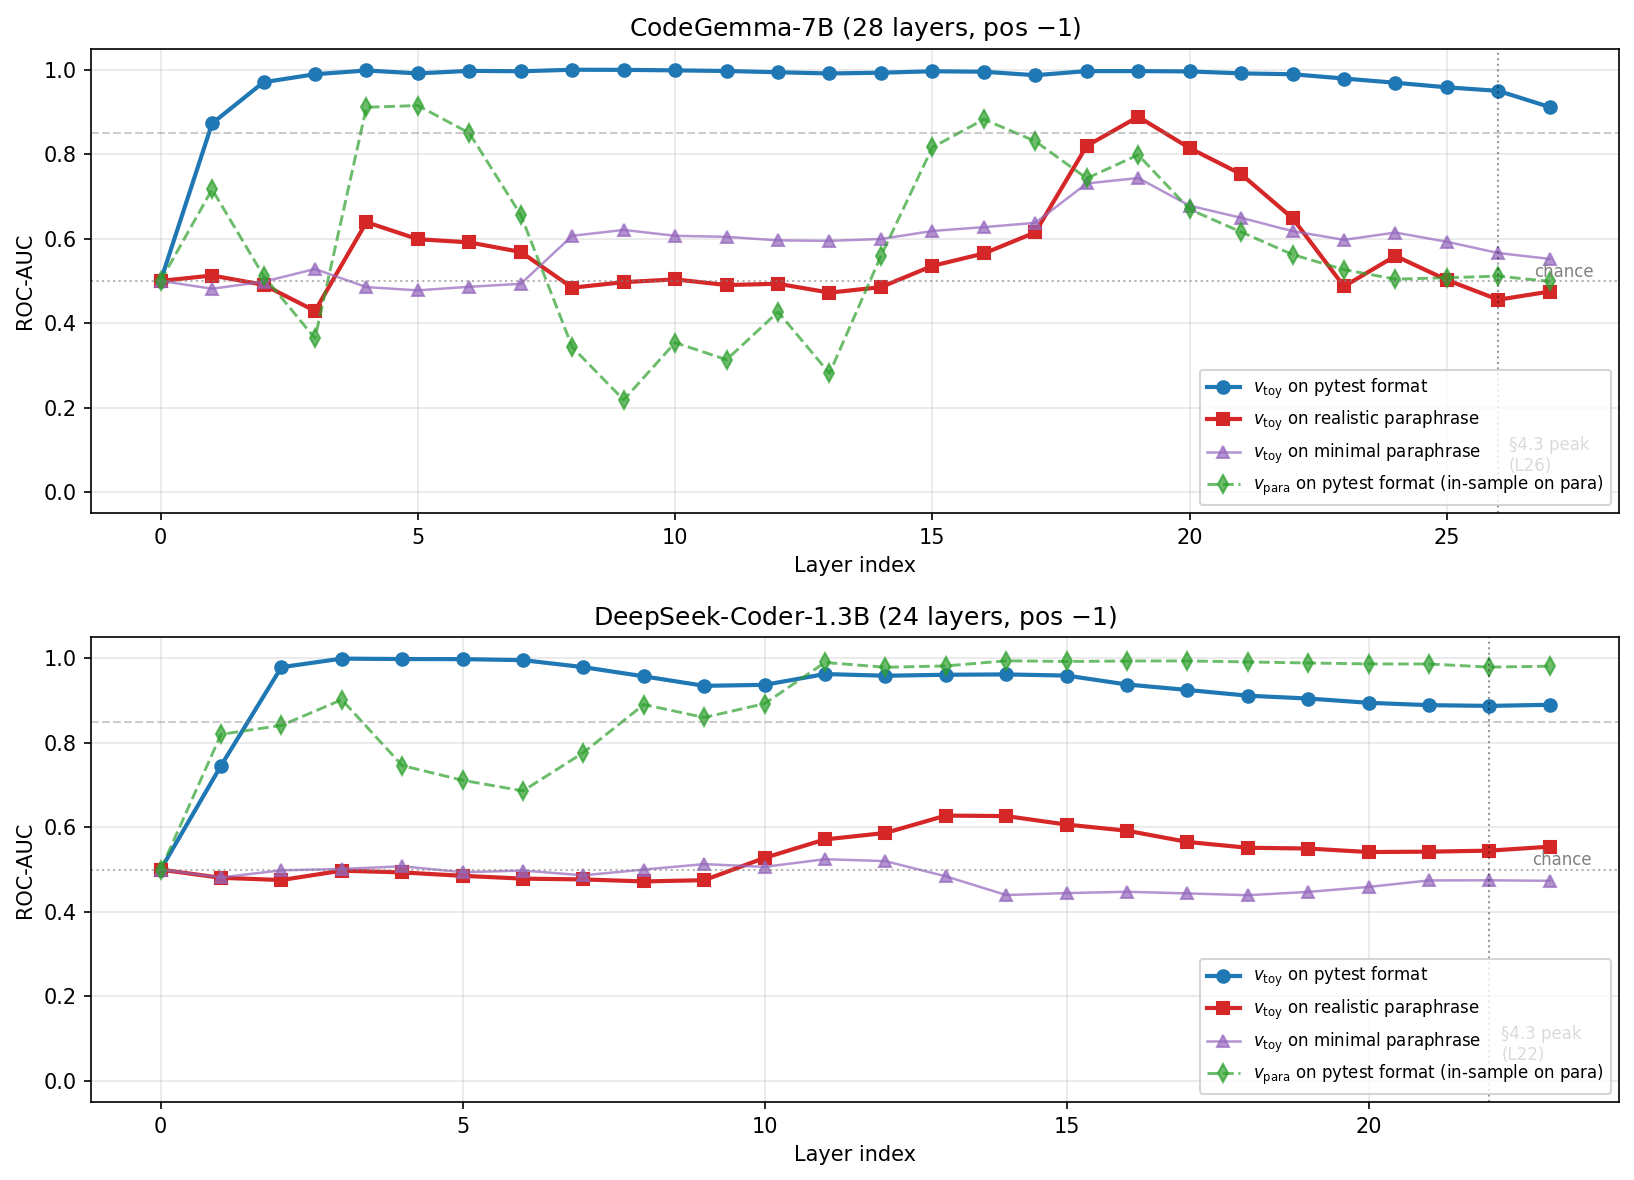
\includegraphics[width=0.99\linewidth,height=\textheight,keepaspectratio,alt={Cross-format layer sweep at pos \ensuremath{-}1 on CodeGemma-7B (top) and DeepSeek-Coder-1.3B (bottom). Blue: v\_\{\textbackslash rm toy\} AUC on pytest format (the paper's canonical methodology). Red: same v\_\{\textbackslash rm toy\} on realistic paraphrase. Green dashed: v\_\{\textbackslash rm para\} (paraphrase-derived) transferred BACK to pytest. Dotted vertical line marks the \S{}4.3 reported cell; on CodeGemma, the reported cell (L26) is NOT the highest cross-format-AUC cell (which sits at L19). On DeepSeek, no v\_\{\textbackslash rm toy\} cell achieves both. Source: scripts/cross\_format\_layer\_sweep.py.}]{figures/cross_format_layer_sweep.png}
\caption{Cross-format layer sweep at pos \ensuremath{-}1 on CodeGemma-7B (top) and
DeepSeek-Coder-1.3B (bottom). Blue: \(v_{\rm toy}\) AUC on pytest format
(the paper's canonical methodology). Red: same \(v_{\rm toy}\) on
realistic paraphrase. Green dashed: \(v_{\rm para}\)
(paraphrase-derived) transferred BACK to pytest. Dotted vertical line
marks the \S{}4.3 reported cell; on CodeGemma, the reported cell (L26) is
NOT the highest cross-format-AUC cell (which sits at L19). On DeepSeek,
no \(v_{\rm toy}\) cell achieves both. Source:
\protect\texttt{scripts/cross\_format\_layer\_sweep.py}.}
\end{figure}

\textbf{Three things this resolves about the G.12 result:}

\begin{enumerate}
\def\labelenumi{\arabic{enumi}.}
\tightlist
\item
  \textbf{A cross-format-discriminative cell can be identified post hoc
  on CodeGemma at L19.} The L26 reported cell is highly discriminative
  on pytest but collapses on the deterministic paraphrase; the L19 cell
  is selected post-hoc for cross-format AUC. Moving the CodeGemma
  \texttt{v\_noop\_cg} derivation to L19 (keeping the toy contrastive
  methodology, just changing the layer) gives a cell with high AUC on
  both formats (pytest 0.997, paraphrase-real 0.888). The L19 cell was
  selected on the paraphrase AUC itself, so this is exploratory evidence
  that such a cell \emph{can be found under post-hoc cell selection} on
  CodeGemma, not held-out validation that the reported cell would have
  found it.
\item
  \textbf{No analogous v\_toy cell exists on DeepSeek at pos \ensuremath{-}1.} No
  layer hosts a \(v_{\rm toy}\) direction with paraphrase-real AUC
  \textgreater{} 0.85. A \(v_{\rm para}\) direction (in-sample on
  paraphrase) does transfer back to pytest, but this is no longer the
  toy-substrate methodology and the in-sample fit prevents claiming an
  abstract representation.
\item
  \textbf{Methodological observation.} Contrastive mean-difference
  directions are sensitive to the format of the contrast data. Toy
  pytest contrasts find a direction discriminative on SWE-derived
  pytest-format prompts (by design); whether they find a format-general
  direction depends on the cell. Validating this methodologically would
  require multi-format toy contrasts evaluated on held-out paraphrases.
\end{enumerate}

We do not retroactively change the \S{}5.1 headline numbers (which use the
\S{}4.3 reported patch cells as anchors and are honest to the paper's
primary methodology). The cross-format layer sweep is reported here as
\textbf{exploratory}: it suggests a cross-format-discriminative cell can
be identified post hoc on CodeGemma, and that an additional methodology
(paraphrase or SWE-derived prompt contrast) is needed to find one on
DeepSeek, without claiming either is a semantic pass/fail direction or
that it generalizes beyond the formats it was selected on.

Outputs:
\texttt{results/monitor\_real/cross\_format\_layer\_sweep\_codegemma.json},
\texttt{cross\_format\_layer\_sweep\_deepseek.json}.

\subsection{Cross-format position sweep (post-hoc, selection-biased):
post-hoc-selected CodeGemma L19/pos=\ensuremath{-}4 and DeepSeek L16/pos=\ensuremath{-}5
cells}\label{cross-format-position-sweep-post-hoc-selection-biased-post-hoc-selected-codegemma-l19pos4-and-deepseek-l16pos5-cells}

G.13 swept layers at pos=\ensuremath{-}1 only. The natural follow-up is the
\textbf{2D sweep}, does some non-canonical position host an even better
cross-format discriminative direction? For each (layer L, position p) in
\(\{-1, -2..., -8\}\), evaluate the three G.13 candidate directions on
all three formats (\texttt{scripts/cross\_format\_position\_sweep.py}).

\textbf{Result, CodeGemma-7B (28 \ensuremath{\times} 8 = 224 cells).} The L19 finding from
G.13 (pos=\ensuremath{-}1) extends naturally to pos=\ensuremath{-}4, where the discrimination
strengthens:

{\def\LTcaptype{none} % do not increment counter
\begin{longtable}[]{@{}llrrr@{}}
\toprule\noalign{}
direction & best cell & pytest & para-real & para-min \\
\midrule\noalign{}
\endhead
\bottomrule\noalign{}
\endlastfoot
\(v_{\rm toy}\) & \textbf{L19 / pos=\ensuremath{-}4} & \textbf{0.976} &
\textbf{0.939} & 0.680 \\
\(v_{\rm toy}\) & L19 / pos=\ensuremath{-}1 (G.13) & 0.997 & 0.888 & 0.744 \\
\(v_{\rm real}\) & L17 / pos=\ensuremath{-}4 & 1.000 (in-sample) & 0.967 & 0.844 \\
\(v_{\rm para}\) & L19 / pos=\ensuremath{-}5 & 0.984 & 1.000 (in-sample) & 0.982 \\
\end{longtable}
}

The cross-format-selected \(v_{\rm toy}\) cell on CodeGemma is (L19,
pos=\ensuremath{-}4) with paraphrase-realistic AUC \textbf{0.939}, up from 0.888 at
pos=\ensuremath{-}1. The \S{}4.3 reported patch cell (L26, pos=\ensuremath{-}1) differs from this
cross-format-selected cell on both axes (7 layers later, 3 positions
earlier), but the reported cell was selected by a different criterion
(toy F\ensuremath{\rightarrow}B/B\ensuremath{\rightarrow}F submargin shift) and we do not read the difference as the
patching result being ``wrong'', it measures a different target than
cross-format discrimination.

\textbf{Result, DeepSeek-Coder-1.3B (24 \ensuremath{\times} 8 = 192 cells).}
\(v_{\rm toy}\) still does \emph{not} recover on DeepSeek at any cell
tested (best para-real AUC under \(v_{\rm toy}\) is \textbf{0.663} at
L8/pos=\ensuremath{-}3). But \(v_{\rm real}\) (derived from the 499 SWE-derived
pytest-format pairs instead of the 49 toy pairs) \textbf{does} recover
at pos=\ensuremath{-}5:

{\def\LTcaptype{none} % do not increment counter
\begin{longtable}[]{@{}
  >{\raggedright\arraybackslash}p{(\linewidth - 8\tabcolsep) * \real{0.2037}}
  >{\raggedright\arraybackslash}p{(\linewidth - 8\tabcolsep) * \real{0.2593}}
  >{\raggedleft\arraybackslash}p{(\linewidth - 8\tabcolsep) * \real{0.1481}}
  >{\raggedleft\arraybackslash}p{(\linewidth - 8\tabcolsep) * \real{0.2037}}
  >{\raggedleft\arraybackslash}p{(\linewidth - 8\tabcolsep) * \real{0.1852}}@{}}
\toprule\noalign{}
\begin{minipage}[b]{\linewidth}\raggedright
direction
\end{minipage} & \begin{minipage}[b]{\linewidth}\raggedright
best cell
\end{minipage} & \begin{minipage}[b]{\linewidth}\raggedleft
pytest
\end{minipage} & \begin{minipage}[b]{\linewidth}\raggedleft
para-real
\end{minipage} & \begin{minipage}[b]{\linewidth}\raggedleft
para-min
\end{minipage} \\
\midrule\noalign{}
\endhead
\bottomrule\noalign{}
\endlastfoot
\(v_{\rm toy}\) & best: L8/pos=\ensuremath{-}3 & 0.998 & 0.663 & 0.483 \\
\textbf{\(v_{\rm real}\)} & \textbf{L16 / pos=\ensuremath{-}5} & 1.000 (in-sample) &
\textbf{0.925} & 0.736 \\
\(v_{\rm real}\) & L10 / pos=\ensuremath{-}5 & 1.000 (in-sample) & 0.920 & 0.770 \\
\(v_{\rm para}\) & L11 / pos=\ensuremath{-}5 & 1.000 & 1.000 (in-sample) & 0.886 \\
\end{longtable}
}

\textbf{Post-hoc diagnosis (cells selected on paraphrase AUC; no
held-out validation):}

\begin{itemize}
\tightlist
\item
  \textbf{CodeGemma}: a \(v_{\rm toy}\) cell at (L19, pos=\ensuremath{-}4) is
  cross-format discriminative at AUC 0.939. The \S{}4.3 reported cell (L26,
  pos=\ensuremath{-}1) was selected by a \emph{different} criterion (toy F\ensuremath{\rightarrow}B/B\ensuremath{\rightarrow}F
  submargin shift), not paraphrase AUC, so the cell mismatch is
  unsurprising.
\item
  \textbf{DeepSeek}: no \(v_{\rm toy}\) cell tested at pos in \{\ensuremath{-}1,
  \ldots, \ensuremath{-}8\} achieves paraphrase-real AUC \textgreater{} 0.67. A
  \(v_{\rm real}\) direction (derived from the 499 SWE-derived
  pytest-format pairs, not 49 toys) at (L16, pos=\ensuremath{-}5) achieves 0.925, but
  this is no longer the same methodology as the canonical toy contrast,
  the ``fix'' is to switch \emph{both} the cell and the contrast data.
\end{itemize}

\begin{figure}
\centering
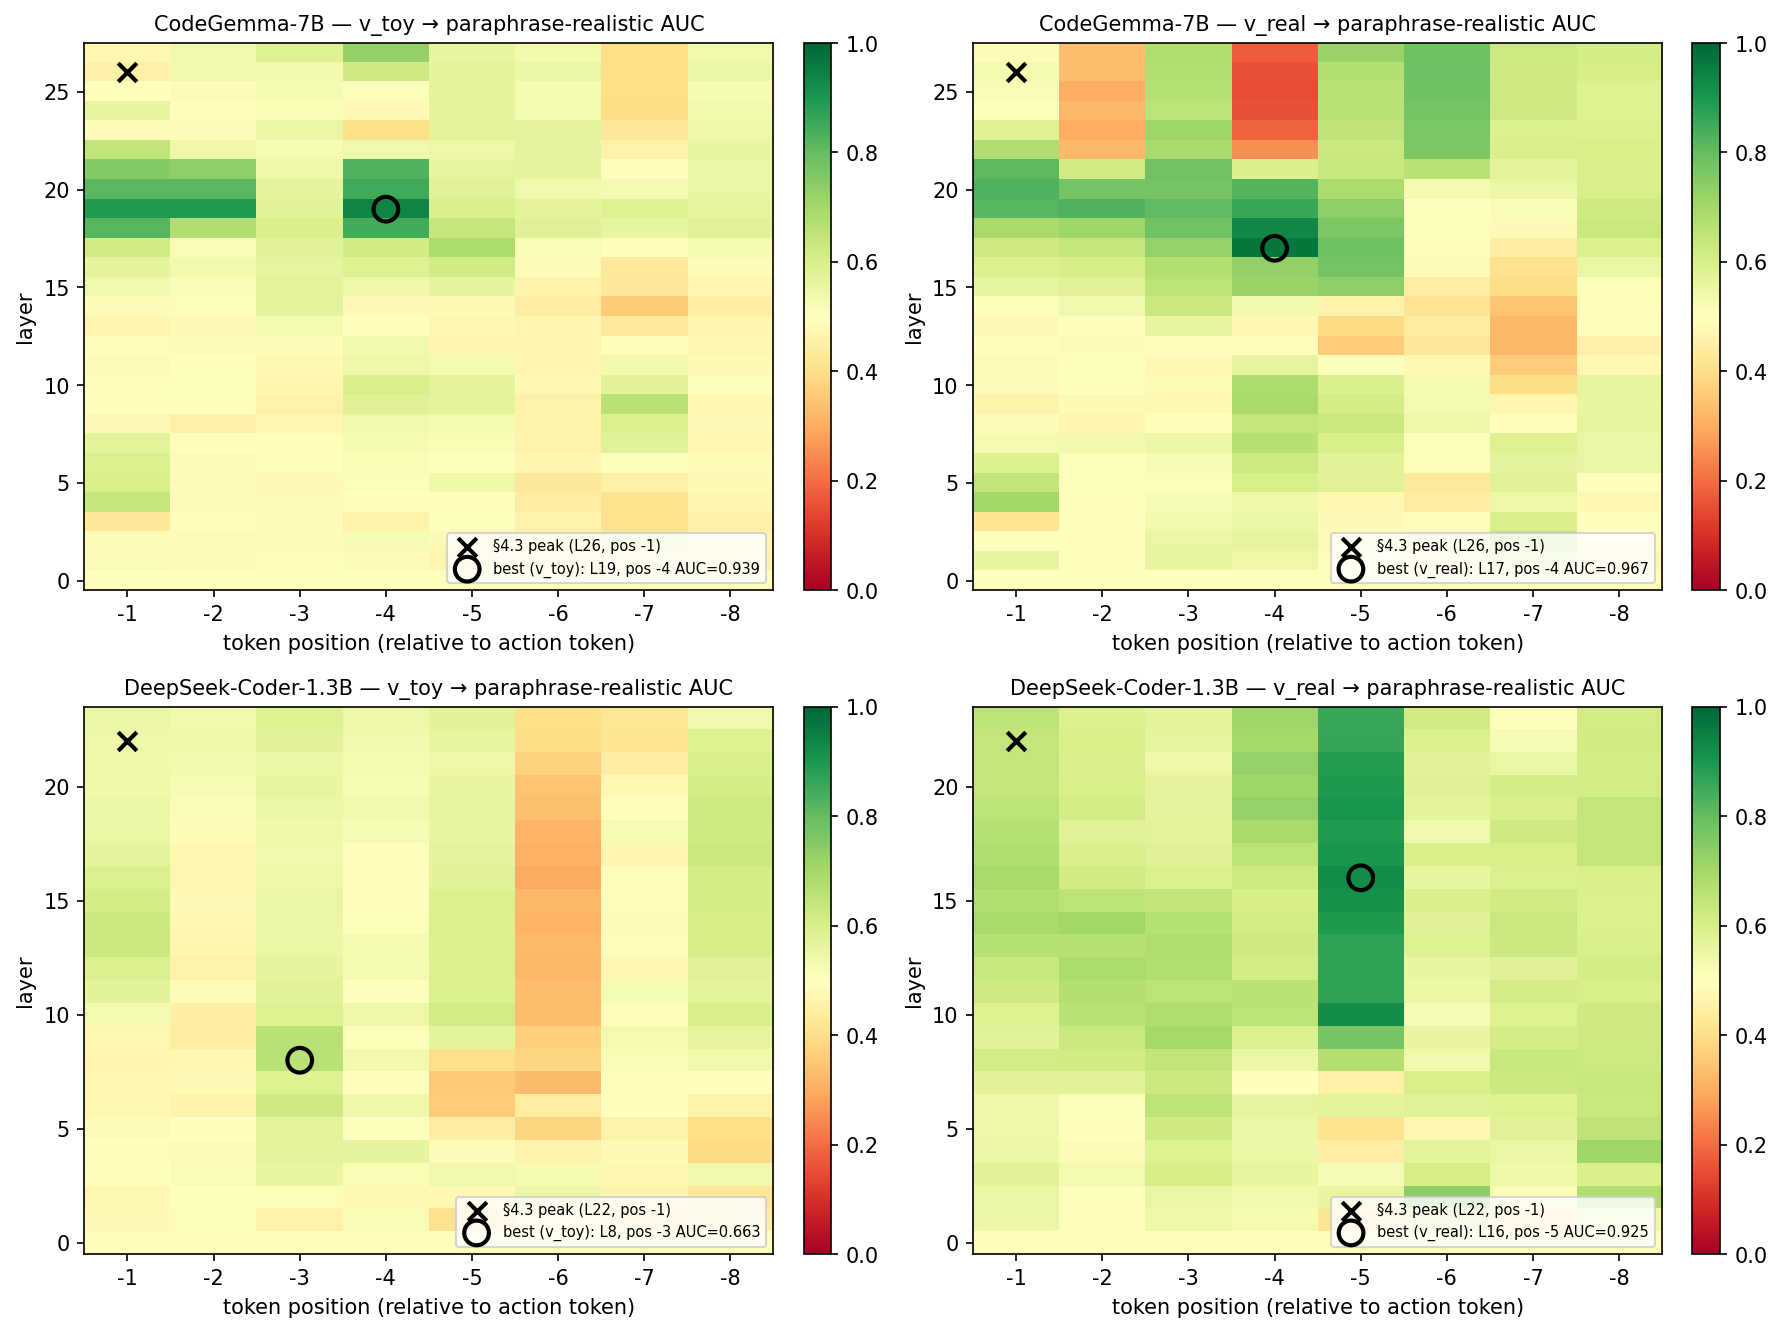
\includegraphics[width=0.99\linewidth,height=\textheight,keepaspectratio,alt={Cross-format position-sweep heatmaps. Cell color = paraphrase-realistic AUC under each direction; black \ensuremath{\times} marks the \S{}4.3 canonical (L\_site, pos=\ensuremath{-}1) reported cell; black circle marks the highest paraphrase-realistic AUC cell. Top row: CodeGemma; bottom row: DeepSeek. Left column: v\_\{\textbackslash rm toy\}; right column: v\_\{\textbackslash rm real\}. On CodeGemma, v\_\{\textbackslash rm toy\} achieves high AUC at the post-hoc selected L19/pos=\ensuremath{-}4 cell (0.939). On DeepSeek, no v\_\{\textbackslash rm toy\} cell tested reaches the 0.85 threshold; v\_\{\textbackslash rm real\} achieves high AUC at the post-hoc selected L16/pos=\ensuremath{-}5 cell (0.925). Source: scripts/cross\_format\_position\_sweep.py.}]{figures/cross_format_position_sweep.png}
\caption{Cross-format position-sweep heatmaps. Cell color =
paraphrase-realistic AUC under each direction; black \ensuremath{\times} marks the \S{}4.3
canonical (L\_site, pos=\ensuremath{-}1) reported cell; black circle marks the
highest paraphrase-realistic AUC cell. Top row: CodeGemma; bottom row:
DeepSeek. Left column: \(v_{\rm toy}\); right column: \(v_{\rm real}\).
On CodeGemma, \(v_{\rm toy}\) achieves high AUC at the post-hoc selected
L19/pos=\ensuremath{-}4 cell (0.939). On DeepSeek, no \(v_{\rm toy}\) cell tested
reaches the 0.85 threshold; \(v_{\rm real}\) achieves high AUC at the
post-hoc selected L16/pos=\ensuremath{-}5 cell (0.925). Source:
\protect\texttt{scripts/cross\_format\_position\_sweep.py}.}
\end{figure}

\textbf{Mechanistic reading (speculative).} The post-hoc-selected cells
with high evaluated-format AUC on CodeGemma and DeepSeek sit at a
non-canonical position (\ensuremath{-}4 / \ensuremath{-}5) at mid-stack layers (L17--L21). The
action-token position (\ensuremath{-}1) at the toy-contrast reported cell picks up a
more \emph{specialised} downstream readout site that is more
format-specific. One reading is that earlier positions (still inside the
prompt tail, before the action-token output) host a less format-bound
representation of the test evidence. We do not have held-out validation
that this reading is correct rather than an artifact of post-hoc cell
selection.

\textbf{Sample-size matters too.} The 49-pair toy contrast finds a
cross-format discriminative cell on Qwen (L24, pos=\ensuremath{-}1) and CodeGemma
(L19, pos=\ensuremath{-}4) but not on DeepSeek. A 499-pair SWE-derived pytest-format
contrast finds one on DeepSeek (L16, pos=\ensuremath{-}5). Suggests the toy-substrate
methodology may be under-powered for some models; scaling to a
SWE-derived prompt contrast addresses it on DeepSeek. Both findings are
post-hoc and need held-out validation.

\textbf{Three-model status after G.13 + G.14:}

\begin{center}
\begin{tabular}{l p{0.46\linewidth} l r}
\toprule
model & status under post-hoc cross-format search & selected cell / dir.\ & AUC \\
\midrule
Qwen & Recovered at canonical Qwen causal cell & L24/$-1$, $v_{\rm toy}$ & 0.995 \\
CodeGemma & Recovered only after post-hoc layer/position search (toy contrast) & L19/$-4$, $v_{\rm toy}$ & 0.939 \\
DeepSeek & Not recovered with toy contrast; only after a SWE-derived pytest-format contrast & L16/$-5$, $v_{\rm real}$ & 0.925 \\
\bottomrule
\end{tabular}
\end{center}

\textbf{The exploratory three-model picture} is that a
cross-format-discriminative cell can be identified post hoc in each
model's residual stream, for Qwen at the canonical causal cell, for
CodeGemma only after a post-hoc layer/position search (the canonical
cell is not the best cross-format readout cell), for DeepSeek only after
switching contrast data. We do \textbf{not} claim the post-hoc cells
generalize to held-out paraphrase formats or to other transcript
distributions; they were selected on the same formats used to evaluate
them. Established more rigorously, this would require: (i)
cross-validated cell selection on one paraphrase format, evaluation on
another; (ii) keyword-regex / BoW baselines at the same cells to
distinguish format-abstract readout from format-keyword readout; (iii)
larger held-out paraphrase suites.

Outputs:
\texttt{results/monitor\_real/cross\_format\_position\_sweep\_codegemma.json},
\texttt{cross\_format\_position\_sweep\_deepseek.json}.

\subsection{Temporally-separated transcript (Qwen): the direction
carries the transcript verdict forward; it beats a stateless turn-local
regex, not a full-history or stateful
parser}\label{temporally-separated-transcript-qwen-the-direction-carries-the-transcript-verdict-forward-it-beats-a-stateless-turn-local-regex-not-a-full-history-or-stateful-parser}

Every result so far places the transcript \emph{adjacent} to the
decision: the pytest output is the last evidence block before the
\texttt{Action:} token. A natural objection is that the mechanism is
then trivial: the model is reading a \texttt{FAILED} token we inserted
deterministically, one block above the readout. This appendix tests
whether the L24/pos \ensuremath{-}1 direction still carries the pass/fail transcript
verdict when the transcript is \textbf{positionally distant} from the
decision, separated by intervening agent turns whose content is
identical across buggy and fixed.

\textbf{Design.} We reformat each of the 499 SWE-derived prompts into a
multi-turn agent trace on Qwen (\texttt{code\_tests\_stale\_multiturn}
in \texttt{src/no\_op\_circuit/dataset/schema.py}):

{\def\LTcaptype{none} % do not increment counter
\begin{longtable}[]{@{}
  >{\raggedright\arraybackslash}p{(\linewidth - 4\tabcolsep) * \real{0.2857}}
  >{\raggedright\arraybackslash}p{(\linewidth - 4\tabcolsep) * \real{0.2857}}
  >{\raggedright\arraybackslash}p{(\linewidth - 4\tabcolsep) * \real{0.4286}}@{}}
\toprule\noalign{}
\begin{minipage}[b]{\linewidth}\raggedright
turn
\end{minipage} & \begin{minipage}[b]{\linewidth}\raggedright
role
\end{minipage} & \begin{minipage}[b]{\linewidth}\raggedright
content
\end{minipage} \\
\midrule\noalign{}
\endhead
\bottomrule\noalign{}
\endlastfoot
1 & user & issue + code + ``what action?'' \\
2 & assistant & \texttt{Action:\ test} \\
3 & user & \textbf{the condition-matched pytest transcript} + ``what
action?'' \\
4 & assistant & \texttt{Action:\ grep} \\
5 & user & \texttt{grep\ -rn\ "TODO"} \ensuremath{\rightarrow} \texttt{(no\ matches\ found)} +
``what action?'' \\
6 & assistant & \texttt{Action:\ view} \\
7 & user & \texttt{CHANGELOG.md} (generic) + ``what action?'' \\
(decision) & assistant & \texttt{Action:} \(\leftarrow\) residual +
action logits read here \\
\end{longtable}
}

Turns 4--7 are \textbf{byte-identical across conditions}. The prompt
still contains buggy/fixed code in turn 1, but the format-matched
no-transcript control below shows that this code difference is not
discriminative for the frozen L24/pos \ensuremath{-}1 linear readout (AUC 0.509); the
additional signal in the 0.807 result is therefore attributable to the
upstream transcript at turn 3. We score with the \textbf{same frozen
toy-trained unit monitor direction \(u_{\rm tx}\)} at (L24, pos \ensuremath{-}1) used
in \S{}5.1, no retraining. The \textbf{format control}
(\texttt{code\_multiturn\_notranscript}) uses the identical scaffold
with the turn-3 transcript replaced by a neutral placeholder
(\texttt{(no\ test\ output\ available)}), holding everything constant
(including the turn-1 code) except the discriminative transcript.

Two regex baselines per prompt: a \textbf{turn-local} regex
(\texttt{"FAILED"} in the \emph{decision-point local context}, the last
user turn, turn 7) and a \textbf{full-scrollback} regex
(\texttt{"FAILED"} anywhere in the rendered prompt). Server-side scoring
returns only per-prompt projections + action logits + regex flags
(\texttt{modal\_app/multiturn\_experiment.py}); CIs are paired-bootstrap
(B=10000, seed=0).

\textbf{Result.}

{\def\LTcaptype{none} % do not increment counter
\begin{longtable}[]{@{}
  >{\raggedright\arraybackslash}p{(\linewidth - 8\tabcolsep) * \real{0.3200}}
  >{\raggedright\arraybackslash}p{(\linewidth - 8\tabcolsep) * \real{0.2000}}
  >{\raggedleft\arraybackslash}p{(\linewidth - 8\tabcolsep) * \real{0.1600}}
  >{\raggedleft\arraybackslash}p{(\linewidth - 8\tabcolsep) * \real{0.1600}}
  >{\raggedleft\arraybackslash}p{(\linewidth - 8\tabcolsep) * \real{0.1600}}@{}}
\toprule\noalign{}
\begin{minipage}[b]{\linewidth}\raggedright
setting
\end{minipage} & \begin{minipage}[b]{\linewidth}\raggedright
transcript position
\end{minipage} & \begin{minipage}[b]{\linewidth}\raggedleft
projection ROC-AUC
\end{minipage} & \begin{minipage}[b]{\linewidth}\raggedleft
turn-local regex AUC
\end{minipage} & \begin{minipage}[b]{\linewidth}\raggedleft
full-scrollback regex AUC
\end{minipage} \\
\midrule\noalign{}
\endhead
\bottomrule\noalign{}
\endlastfoot
\S{}5.1 (adjacent) & last block before decision & \textbf{0.989} & 1.000 &
1.000 \\
\textbf{\texttt{code\_tests\_stale\_multiturn}} & \textbf{turn 3, behind
2 turns} & \textbf{0.807} {[}0.788, 0.827{]} & \textbf{0.500} & 1.000 \\
\texttt{code\_multiturn\_notranscript} (control) & absent
(format-matched) & 0.509 {[}0.494, 0.525{]} & 0.500 & 0.500 \\
\S{}G.9 (1-turn, no transcript) & absent & \ensuremath{\leq} 0.52 & -- & -- \\
\end{longtable}
}

\textbf{The transcript verdict survives the temporal separation.} With
the transcript pushed two agent turns + the intervening tokens upstream,
and the decision-point's local context containing \textbf{no pass/fail
tokens at all}, the frozen direction still discriminates the
failing-transcript (buggy) from the passing-transcript (fixed) condition
at \textbf{AUC 0.807} (CI excludes both chance and the format control).
The signal degrades from the adjacent 0.989 (dilution across the
intervening turns is expected) but stays far above the \textbf{0.509}
format control and the \S{}G.9 no-transcript floor. The control's chance
AUC confirms the multi-turn \emph{format} does not by itself create
discriminability, the 0.807 is the carried-forward transcript signal.

\textbf{This beats a stateless turn-local regex (only).} A
\textbf{stateless turn-local} regex, one inspecting only the current
observation before deciding the next action, reads \textbf{chance
(0.500)}, because the decision-local context contains no \texttt{FAILED}
token: it is two turns upstream. The residual projection carries the
transcript verdict to the decision point where a stateless local parser
sees nothing. It does \textbf{not} beat a \textbf{full-history} regex or
a \textbf{stateful} parser that records earlier test outcomes: a
full-scrollback regex (re-scanning the entire context) still recovers
AUC 1.000 here, and a stateful parser would simply store the turn-3
test-output verdict. The result's value is therefore
\textbf{mechanistic}: it shows the model carries the upstream transcript
verdict forward to the final action position, \textbf{not} deployment
superiority over text parsing.

\textbf{The action hides what the residual reveals.} In the stale-
multiturn setting Qwen's first-token argmax distribution is
\textbf{identical across conditions}, buggy: 173 \texttt{edit} / 326
\texttt{grep}; fixed: 173 \texttt{edit} / 326 \texttt{grep}, yet the
projection separates the two at 0.807. The emitted action carries
\emph{no} information about the pass/fail transcript verdict here
(consistent with the paper's 0\% noop / action-prior-dominance story);
the residual carries it anyway. This is the cleanest demonstration in
the paper that the direction reads evidence the behavior does not
surface.

\textbf{Scope.} This is \textbf{Qwen-only} and a \textbf{single forward
pass} over a constructed multi-turn prompt, not a live agent loop with
KV-cache continuation or context eviction; ``temporally separated'' here
means positionally distant within one rendered context, with the
transcript still textually present (hence the full-history regex still
recovers it). A genuinely \emph{evicted} transcript (truncated out of
the context window) cannot be read from a single-pass residual, that is
the \S{}G.9 no-transcript regime, which is negative. The contribution is
\textbf{mechanistic}: the L24 direction carries the upstream transcript
verdict to the final action position, which rebuts the
adjacent-keyword-triviality reading. We do \textbf{not} claim
operational superiority over text parsing: the residual beats only a
stateless turn-local regex, not a full-history regex or a stateful
parser that records test outcomes as they appear.

Outputs: \texttt{results/monitor\_real/multiturn\_experiment\_*.json};
variants \texttt{code\_tests\_stale\_multiturn} /
\texttt{code\_multiturn\_notranscript} in
\texttt{src/no\_op\_circuit/dataset/schema.py};
\texttt{modal\_app/multiturn\_experiment.py},
\texttt{scripts/analyze\_multiturn.py}.

\subsection{Cross-model contradictory-transcript control: full 2 \ensuremath{\times} 2 on
CodeGemma and
DeepSeek}\label{cross-model-contradictory-transcript-control-full-2-2-on-codegemma-and-deepseek}

\S{}5.2's contradictory-transcript control, the keystone ``reads
transcript, not code'' result, was originally Qwen-only. This appendix
runs the same control on CodeGemma-7B and DeepSeek-1.3B with the
\textbf{identical} 2 \ensuremath{\times} 2 (code \ensuremath{\times} transcript) design and statistics.

\textbf{Method.} For each of the 499 SWE-bench-Verified-derived tasks we
forward all four cells fresh on the GPU (server-side scoring, so only a
small per-cell JSON returns, no large-tensor download competing with
other transfers):

{\def\LTcaptype{none} % do not increment counter
\begin{longtable}[]{@{}llll@{}}
\toprule\noalign{}
cell & code & transcript & variant / condition \\
\midrule\noalign{}
\endhead
\bottomrule\noalign{}
\endlastfoot
BB & buggy & failing & \texttt{code\_tests} / buggy \\
FF & fixed & passing & \texttt{code\_tests} / fixed \\
BF & buggy & passing & \texttt{code\_tests\_swapped} / buggy \\
FB & fixed & failing & \texttt{code\_tests\_swapped} / fixed \\
\end{longtable}
}

Each cell is scored with the model's frozen toy-trained unit monitor
direction \(u_{\rm tx}\) at its \S{}4.3 reported patch cell (CodeGemma L26,
the \textbf{all-49} direction matching the \S{}5.1 headline, \ensuremath{\|}v\ensuremath{\|}=6.181;
DeepSeek L22, \ensuremath{\|}v\ensuremath{\|}=12.255), \texttt{score\ =\ \ensuremath{-}projection}. CodeGemma
applies the same 2400-token cap as \S{}5.1 (a few over-long cells drop,
leaving N=496 tasks present in all four cells; DeepSeek N=499). \ensuremath{\Delta}Code,
\ensuremath{\Delta}Transcript, the interaction, and bootstrap CIs (B=10000, seed=0) use
the identical formulas as
\texttt{scripts/contradictory\_transcript\_analysis.py}.

\textbf{Full 2 \ensuremath{\times} 2 cell means} (score = \ensuremath{-}projection; higher = more
buggy-like):

{\def\LTcaptype{none} % do not increment counter
\begin{longtable}[]{@{}lrr@{}}
\toprule\noalign{}
cell & CodeGemma-7B & DeepSeek-1.3B \\
\midrule\noalign{}
\endhead
\bottomrule\noalign{}
\endlastfoot
(B,B) buggy code + failing tx & +8.307 & \ensuremath{-}13.164 \\
(B,F) buggy code + passing tx & +5.398 & \ensuremath{-}18.854 \\
(F,B) fixed code + failing tx & +8.338 & \ensuremath{-}13.104 \\
(F,F) fixed code + passing tx & +5.460 & \ensuremath{-}18.808 \\
\end{longtable}
}

The two failing-transcript cells (B,B and F,B) cluster together and the
two passing-transcript cells (B,F and F,F) cluster together,
\emph{regardless of the code}, exactly the signature of a
transcript-driven readout. The main-effect decomposition and
swapped-only AUCs are in \S{}5.2's cross-model table; the headline is that
on both models \ensuremath{\Delta}Transcript dominates (CodeGemma +2.894, DeepSeek
+5.697), \textbar \ensuremath{\Delta}Code\textbar{} \ensuremath{\leq} 0.06, and the swapped-only
transcript AUC (0.951 / 0.888) far exceeds the code AUC (0.049 / 0.112).
Argmax-action distributions per cell are in the output JSON.

Outputs:
\texttt{results/monitor\_real/contradictory\_crossmodel\_20260520T034649Z.json};
\texttt{modal\_app/contradictory\_crossmodel.py},
\texttt{scripts/analyze\_contradictory\_crossmodel.py}; CodeGemma all-49
direction \texttt{results/v\_noop\_codegemma\_all49.pt}. The Qwen \S{}5.2
analysis uses
\texttt{results/monitor\_real/contradictory\_transcript\_2x2.json},
\texttt{scripts/contradictory\_transcript\_analysis.py}, the
\texttt{code\_tests\_swapped} variant + flip\_tests scaffolding in
\texttt{src/no\_op\_circuit/dataset/schema.py} and
\texttt{src/no\_op\_circuit/agent/prompt.py}, and Modal cache run
\texttt{results/cache-real-qwen-swap-n500-20260518T074930Z/}.

\subsection{Held-out paraphrase robustness: Qwen positive,
CodeGemma/DeepSeek negative at reported
cells}\label{held-out-paraphrase-robustness-qwen-positive-codegemmadeepseek-negative-at-reported-cells}

The \S{}G.12 deterministic paraphrase is keyword-leaky: a regex tuned to
its vocabulary reaches AUC 1.0. We run a stricter \textbf{template-based
held-out} robustness test on Qwen. We author two \emph{train} paraphrase
templates and two \emph{held-out} templates (A, B) and check overlap
automatically: under lowercase / \texttt{{[}a-z{]}+}-tokenization /
stopword-and-structural-word stripping, there is \textbf{no shared
discriminative content vocabulary} (empty intersection; train words
\texttt{\{wrong,\ right,\ diverged,\ matched,\ breaks,\ fulfills...\}}
vs held-out
\texttt{\{violation,\ contradicted,\ honored,\ open,\ closed,\ discrepancy,\ consistent...\}});
functional words and template structure may still leak weak cues. We
render the 499 SWE-derived paired prompts under each family (499 buggy +
499 fixed per family), score the \textbf{frozen} toy-trained Qwen
\(u_{\rm tx}\) at L24/pos \ensuremath{-}1 with \textbf{no} held-out
cell/threshold/direction selection, and compare against text baselines
fit \textbf{only} on train-template text. Positive class is the matched
failing-transcript/buggy condition.

\begin{center}
\setlength{\tabcolsep}{4pt}
\resizebox{\linewidth}{!}{%
\begin{tabular}{l c r r r r}
\toprule
classifier & fit on held-out? & held-out A AUC & held-out B AUC & pooled AUC & pooled AP \\
\midrule
frozen Qwen $u_{\rm tx}$ (L24/pos $-1$) & no & 0.905 & 0.983 & \textbf{0.943} & 0.932 \\
literal-\texttt{FAILED} regex & no & 0.500 & 0.500 & 0.500 & 0.500 \\
train-vocabulary keyword rule & no & 0.500 & 0.500 & 0.500 & 0.500 \\
BoW logistic (train$\to$held-out) & no & 1.000$^\ast$ & 1.000$^\ast$ & 0.750 & 0.833 \\
\bottomrule
\end{tabular}}
\end{center}

\(^\ast\)The per-template BoW AUC is \textbf{degenerate}: a text
baseline sees only each template's two constant transcript strings (four
distinct strings total), so per-template AUC merely reflects whether
those two strings are ordered correctly. The residual monitor's
per-template AUCs are not degenerate in the same way because the
residual varies across full prompts, whereas the text-only BoW baseline
sees only two transcript strings per held-out template. The
\textbf{pooled} column is therefore the fair head-to-head. (Frozen
\(u_{\rm tx}\) reaches AUC 0.994 on the train-template family; its mean
failing-minus-passing classifier-score gap on held-out is +2.60 on A and
+3.82 on B.) The frozen direction generalizes to
disjoint-content-vocabulary held-out paraphrases at pooled AUC 0.943,
above the literal-token and train-vocabulary keyword baselines (both
exactly at chance, as expected when the discriminative words are held
out) and above the train-fit BoW (pooled 0.750). The BoW result should
be interpreted cautiously rather than dismissed: it orders each held-out
template's two strings (per-template AUC 1.0, the degenerate
within-template comparison above) but its cross-template calibration is
inconsistent (pooled AUC 0.750, held-out prediction spread 0.108),
consistent with weak functional-word / template-structure residue rather
than robust lexical transfer. It is therefore the strongest
no-held-out-fitting text baseline we evaluated in this template setup,
but it should not be read as a general-purpose held-out paraphrase
baseline. This is \textbf{preliminary, template-based} evidence of
held-out paraphrase robustness \emph{on Qwen only}; we do \textbf{not}
claim a semantic pass/fail abstraction, because the held-out set is two
hand-authored deterministic templates (not adversarial or
LLM-generated).

\textbf{Cross-model reported-cell follow-up (CodeGemma, DeepSeek): the
held-out robustness is Qwen-specific.} We rerun the identical templates
and text baselines on CodeGemma and DeepSeek, scoring each model's
\textbf{frozen toy-trained direction at its \S{}4.3 reported cell}
(CodeGemma L26/pos \ensuremath{-}1, all-49 direction; DeepSeek L22/pos \ensuremath{-}1) with
\textbf{no post-hoc layer/position search}. The text baselines are
model-independent (they see only the transcript text):
literal-\texttt{FAILED} 0.500, train-vocabulary keyword 0.500, BoW
(train\ensuremath{\rightarrow}held-out) pooled 0.750 throughout. For each model, the pooled
held-out set contains 499 paired tasks split across held-out templates A
and B (250 and 249 tasks respectively), i.e.~998 total prompts; the
pooled held-out AUC pools templates A and B, and the per-template
``held-out A / B'' columns are computed over the 250 and 249 matched
failing/passing pairs, respectively. All three models use the full 499
paired tasks here with no token-cap drops (the short paraphrase prompts
do not hit the cap that reduced CodeGemma to 497 in \S{}5.1). Audit:
\texttt{scripts/audit\_heldout\_paraphrase\_counts.py} \ensuremath{\rightarrow}
\texttt{results/heldout\_paraphrase\_robustness/count\_audit.\{json,md\}}.

{\def\LTcaptype{none} % do not increment counter
\begin{longtable}[]{@{}
  >{\raggedright\arraybackslash}p{(\linewidth - 6\tabcolsep) * \real{0.2000}}
  >{\raggedleft\arraybackslash}p{(\linewidth - 6\tabcolsep) * \real{0.2667}}
  >{\raggedleft\arraybackslash}p{(\linewidth - 6\tabcolsep) * \real{0.2667}}
  >{\raggedleft\arraybackslash}p{(\linewidth - 6\tabcolsep) * \real{0.2667}}@{}}
\toprule\noalign{}
\begin{minipage}[b]{\linewidth}\raggedright
model (reported cell)
\end{minipage} & \begin{minipage}[b]{\linewidth}\raggedleft
residual train-template AUC
\end{minipage} & \begin{minipage}[b]{\linewidth}\raggedleft
residual held-out pooled AUC
\end{minipage} & \begin{minipage}[b]{\linewidth}\raggedleft
held-out A / B
\end{minipage} \\
\midrule\noalign{}
\endhead
\bottomrule\noalign{}
\endlastfoot
Qwen (L24/pos \ensuremath{-}1) & 0.994 & \textbf{0.943} & 0.905 / 0.983 \\
CodeGemma (L26/pos \ensuremath{-}1) & 0.917 & 0.649 & 0.645 / 0.660 \\
DeepSeek (L22/pos \ensuremath{-}1) & 0.567 & 0.619 & 0.792 / 0.454 \\
\end{longtable}
}

Only Qwen's frozen direction generalizes to the held-out templates
(0.943, above the BoW 0.750). CodeGemma's direction holds on its own
train templates (0.917) but degrades sharply on held-out (0.649, below
the model-independent BoW 0.750); DeepSeek's collapses (held-out pooled
0.619, and \emph{below chance} on template B), and is weak even on train
templates (0.567). This matches the \S{}G.12 finding that the
CodeGemma/DeepSeek directions are more pytest-format-specific, and
confirms that held-out paraphrase robustness here is a
\textbf{Qwen-specific} property of the reported-cell direction, not a
cross-model one. CodeGemma's 0.917 train-template AUC is measured on the
new G.17 train-template family; it should not be compared directly to
the G.12 deterministic realistic-paraphrase cell where the reported-cell
direction inverted.

\textbf{Held-out operating points (threshold frozen on train
templates).} Fixing each model's balanced-accuracy threshold on its
train-template prompts and applying it unchanged to the held-out
templates (CPU reanalysis of the same score artifacts, no model
forwards;
\texttt{scripts/held\_out\_threshold\_calibration\_crossmodel.py} \ensuremath{\rightarrow}
\texttt{results/monitor\_real/held\_out\_threshold\_calibration\_crossmodel.\{json,md\}})
gives a true out-of-sample operating point. Qwen holds (held-out
precision 0.868, recall 0.900, fixed-condition FPR 0.136, accuracy
0.882), whereas CodeGemma (precision 0.609, recall 0.571, FPR 0.367,
accuracy 0.602) and DeepSeek (precision 0.611, recall 0.611, FPR 0.389,
accuracy 0.611) fall to near-chance operating points, consistent with
their collapsed held-out AUC. This is the paraphrase-setting held-out
calibration and is not a substitute for a \S{}5.1 canonical-menu
calibration table: the raw \S{}5.1 per-task projection caches are not
retained locally, so reproducing the canonical-menu random-split /
leave-one-repo-out classifier table for CodeGemma and DeepSeek would
require re-running model forwards, which we leave as future work.

Artifacts and the exact preprocessing / vocabulary-overlap report are in
App. J
(\texttt{results/heldout\_paraphrase\_robustness/\{qwen,codegemma,deepseek\}\_summary.json}).

\section{SAE decomposition: full
analysis}\label{sae-decomposition-full-analysis}

\begin{figure}
\centering
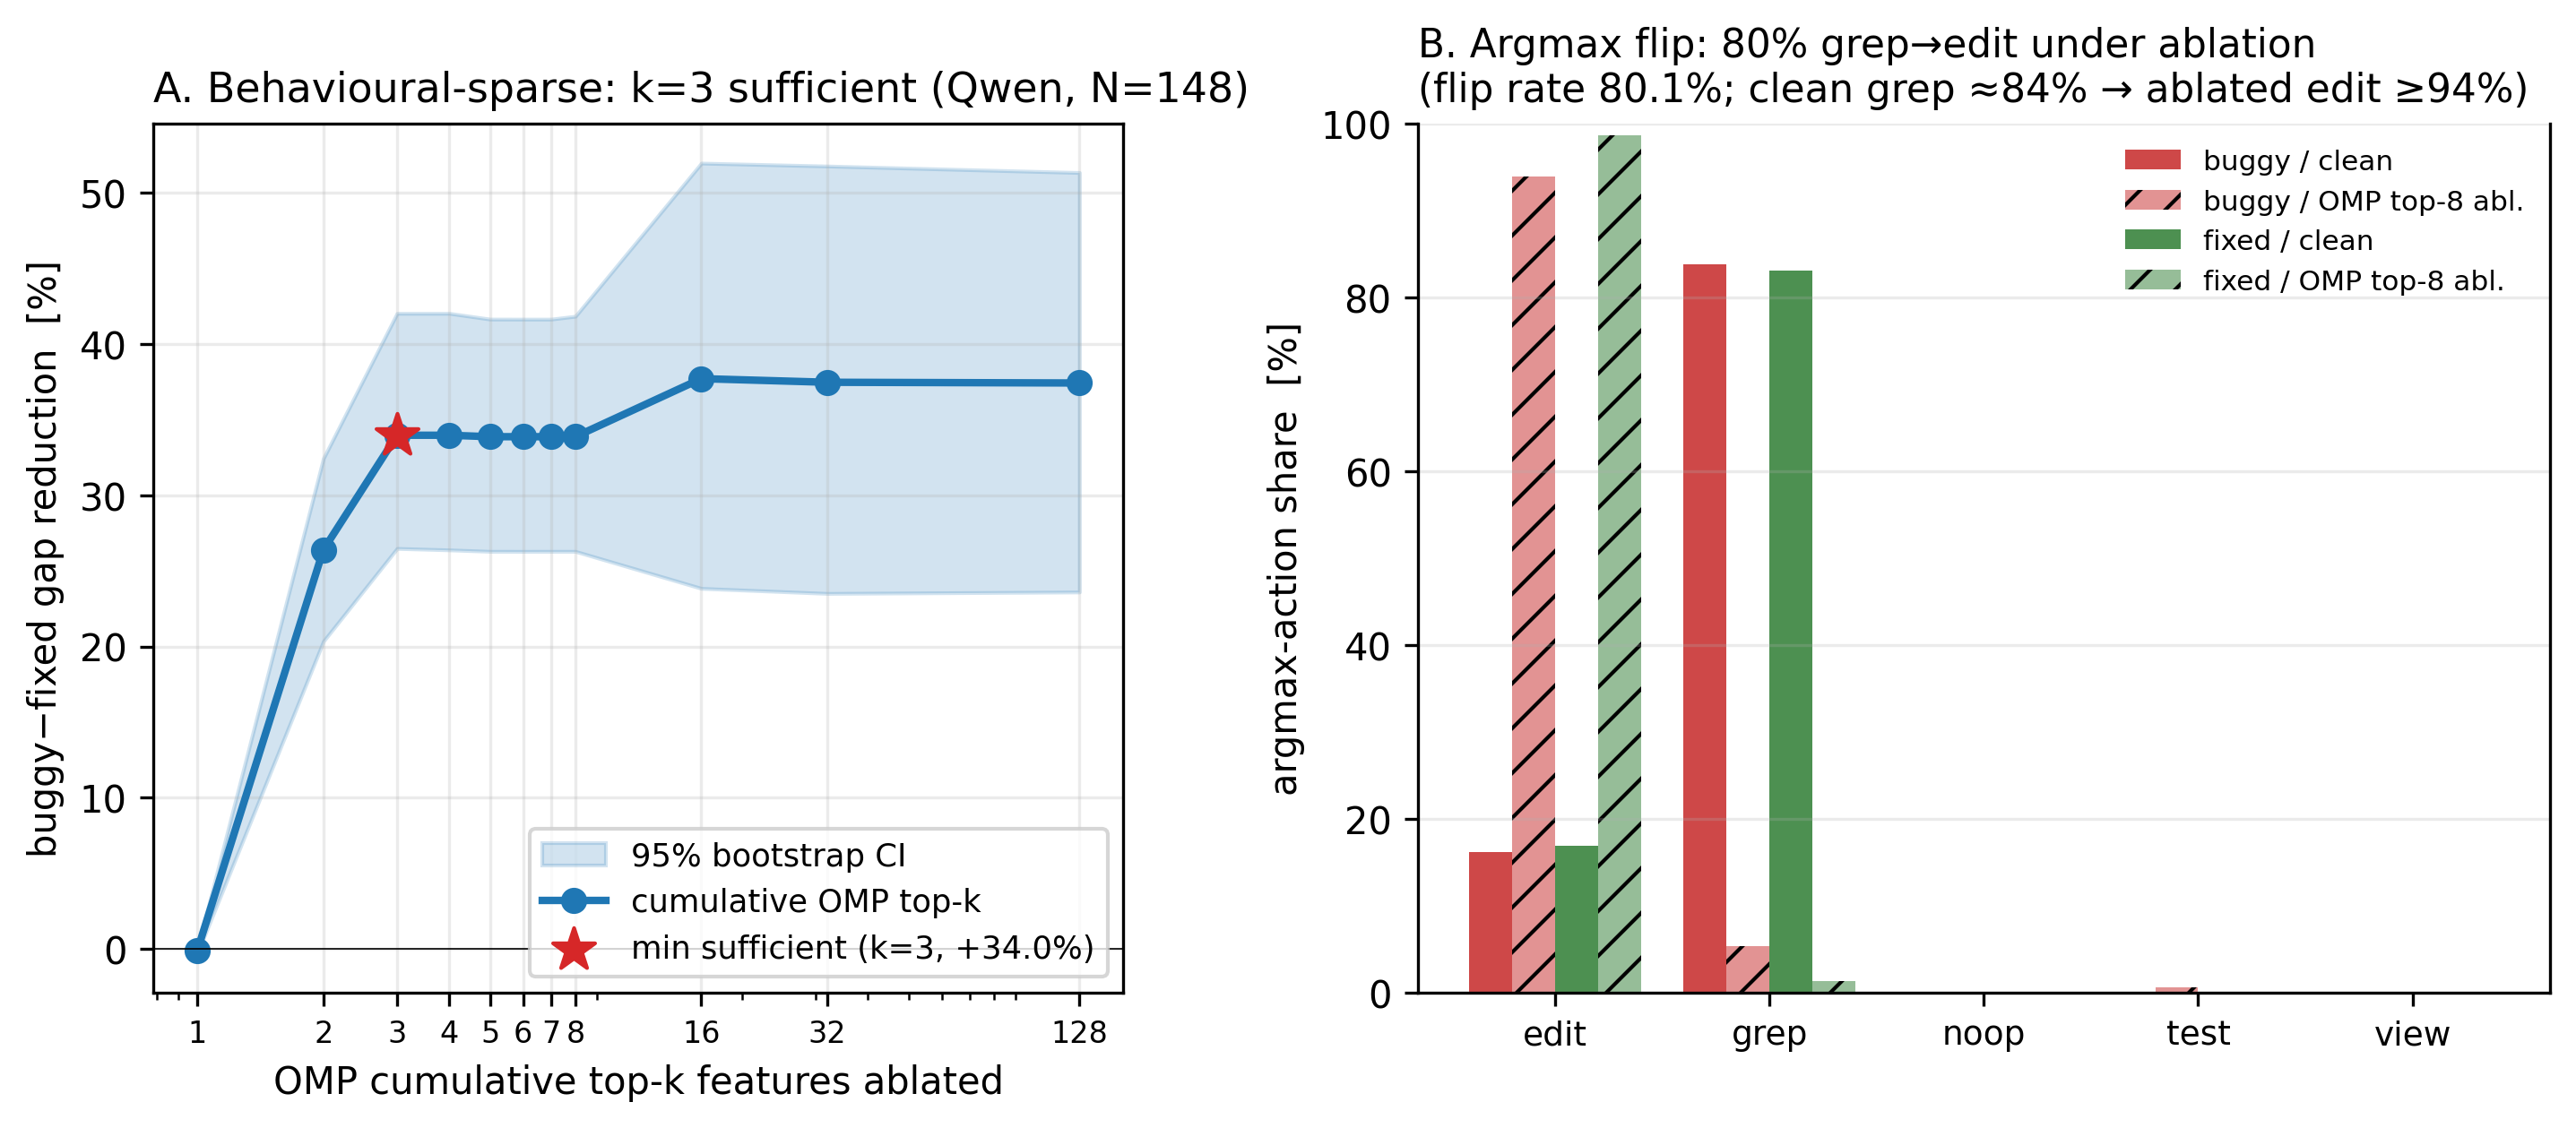
\includegraphics[width=0.98\linewidth,height=\textheight,keepaspectratio,alt={SAE decomposition (exploratory) on Qwen. (A) Cumulative top-k OMP ablation of the original seed-unknown artifact reduces the buggy/fixed margin gap by 0\% at k=1, +26.4\% at k=2, and reaches +34.0\% at k=3 (95\% paired-bootstrap CI shaded); the magnitude is seed-fragile (App. H.7 reports +30.3\% at k=2 under seed=0, plateau ending at k=5). (B) Argmax-action distribution before vs after OMP top-8 ablation on 296 paired buggy/fixed prompts: clean Qwen prefers grep (\textasciitilde84\%); ablating the OMP top-8 features flips 80.1\% of prompts (237/296), 236/237 grep \ensuremath{\rightarrow} edit, one grep \ensuremath{\rightarrow} test, an action-prior override toward edit, not noop. The \S{}5.2 control re-interprets the ablated features as pass/fail-transcript-text features. Both numbers are seed-fragile (App. H.7); CodeGemma replication: geometric pattern holds, behavioral specificity does not (App. H.6).}]{figures/main_sae.png}
\caption{\textbf{SAE decomposition (exploratory) on Qwen.} \emph{(A)}
Cumulative top-k OMP ablation of the original seed-unknown artifact
reduces the buggy/fixed margin gap by 0\% at k=1, +26.4\% at k=2, and
reaches +34.0\% at k=3 (95\% paired-bootstrap CI shaded); the magnitude
is seed-fragile (App. H.7 reports +30.3\% at k=2 under seed=0, plateau
ending at k=5). \emph{(B)} Argmax-action distribution before vs after
OMP top-8 ablation on 296 paired buggy/fixed prompts: clean Qwen prefers
\protect\texttt{grep} (\textasciitilde84\%); ablating the OMP top-8
features flips \textbf{80.1\%} of prompts (237/296), 236/237
\protect\texttt{grep\ \ensuremath{\rightarrow}\ edit}, one \protect\texttt{grep\ \ensuremath{\rightarrow}\ test}, an
action-prior override toward \protect\texttt{edit}, not
\protect\texttt{noop}. The \S{}5.2 control re-interprets the ablated
features as pass/fail-transcript-text features. Both numbers are
seed-fragile (App. H.7); CodeGemma replication: geometric pattern holds,
behavioral specificity does not (App. H.6).}\label{fig:sae}
\end{figure}

\subsection{Setup and geometric
finding}\label{setup-and-geometric-finding}

\textbf{Corpus accounting.} The SAE corpus uses three different counts
of ``prompt'' that we summarize here once to avoid confusion:

{\def\LTcaptype{none} % do not increment counter
\begin{longtable}[]{@{}
  >{\raggedright\arraybackslash}p{(\linewidth - 4\tabcolsep) * \real{0.4000}}
  >{\raggedleft\arraybackslash}p{(\linewidth - 4\tabcolsep) * \real{0.0952}}
  >{\raggedright\arraybackslash}p{(\linewidth - 4\tabcolsep) * \real{0.5048}}@{}}
\toprule\noalign{}
\begin{minipage}[b]{\linewidth}\raggedright
unit
\end{minipage} & \begin{minipage}[b]{\linewidth}\raggedleft
count
\end{minipage} & \begin{minipage}[b]{\linewidth}\raggedright
role
\end{minipage} \\
\midrule\noalign{}
\endhead
\bottomrule\noalign{}
\endlastfoot
Paired toy tasks & \textbf{49} & substrate for \S{}4 patching, steering,
\(u_{\rm tx}\) derivation \\
Toy \texttt{(task,\ variant)} cells in SAE cache & varied & training
input is residual positions, not prompts \\
Total prompts in SAE training corpus & \textbf{1282} & union of all
cached prompts across all variants \\
Residual positions in training corpus & \textbf{1.23M} & streaming SAE
training operates on these \\
Paired \texttt{(task,\ variant)} pairs with both \texttt{buggy} and
\texttt{fixed} materialized & \textbf{148} & used for the H.2--H.4
ablation evaluation \\
Paired buggy/fixed prompts in ablation eval & \textbf{296} & = 148 \ensuremath{\times}
\{buggy, fixed\} \\
\end{longtable}
}

The arithmetic 49 \ensuremath{\times} 5 variants \ensuremath{\times} 2 conditions = 490 prompts is the
theoretical maximum if every \texttt{(task,\ variant)} cell had both
conditions materialized. The actual cache had 1282 prompts because some
variants were materialized multiple times during pipeline iteration
(older prompt-template runs in the cache root). Of those, 148
\texttt{(task,\ variant)} cells have both \texttt{buggy} and
\texttt{fixed} versions, and those 296 prompts (148 \ensuremath{\times} 2) are the
ablation evaluation set.

\textbf{Caveat on the SAE training corpus.} Because the SAE analysis is
treated as \textbf{exploratory} (App. H.7 establishes the precise
plateau magnitudes are seed-fragile), we did \textbf{not} deduplicate
the 1282-prompt cache before training, and we did not re-train on a
clean 296- or 490-prompt corpus. The cache may contain multiple
materializations of the same \texttt{(task,\ variant,\ condition)} under
slightly different prompt-template versions used during pipeline
iteration. None of this paper's causal claims (\S{}4) or monitor claims
(\S{}5.1--\S{}5.2, App. G) depend on this corpus; they use only the residual
at L24/pos \ensuremath{-}1 from a clean re-run. A clean-corpus SAE re-train remains
future work.

We trained a TopK SAE
\citep{gao2024scaling, bricken2023monosemanticity, templeton2024scaling}
on Qwen2.5-Coder-1.5B L24 \texttt{resid\_pre} activations cached over
the 1282-prompt toy corpus, 1.23M residual positions, streaming.
Architecture: d\_in = 1536, d\_sae = 4096, k = 16. The SAE reached
explained variance EV = 0.976 with 16.0 mean active features and a
0.02\% dead-feature rate after 8 epochs on a Modal A10G (73 s training,
\textasciitilde\$0.02). This corpus was chosen after a generic
Python-only SAE (d\_sae = 24,576, k = 32, EV = 0.954 on
\texttt{bigcode/the-stack-smol}) reconstructed the contrast direction
with cosine only +0.21: the action-position residual after a
chat-templated agent prompt is out of distribution for mid-Python-file
activations.

\textbf{The contrast direction is geometrically dense in the SAE basis.}
On the task-distribution SAE the encoder TopK reconstruction of the
contrast direction is poor (cos = +0.10 at k = 16, the trained
sparsity). To separate ``the encoder is suboptimal for OOD directions''
from ``the direction is intrinsically dense in this basis,'' we evaluate
\textbf{orthogonal matching pursuit (OMP)}, a greedy k-sparse
reconstruction procedure that iteratively selects decoder columns and
refits coefficients by least squares (greedy, not globally optimal). The
``OMP-then-ablate'' sequence is the manual analog of
automated-circuit-discovery methods such as ACDC \citep{conmy2023acdc}.
OMP needs k \ensuremath{\approx} 128 features to reach cos \ensuremath{\geq} 0.80 (task SAE 0.806; generic
SAE 0.838) and k \ensuremath{\approx} 256 to clear cos \ensuremath{\geq} 0.85 (task 0.900; generic 0.947)
on either SAE. The basis itself spans the full input space (dense
least-squares cosine = 1.000), so this is not a capacity bug,
\(u_{\rm tx}\) simply does not admit a small-k sparse expansion.
Encoder-TopK underperforms OMP by 0.2--0.4 cosine at every k, indicating
that the trained encoder biases are tuned to typical residuals (norm
\textasciitilde30) and degrade for steering directions of small
magnitude (\(\|v_{\rm raw}\|\) = 5.89).

\subsection{Cumulative top-k ablation on the original SAE
artifact}\label{cumulative-top-k-ablation-on-the-original-sae-artifact}

A fine-grained cumulative sweep over k \ensuremath{\in} \{1, 2, \ldots, 8, 16, 32,
128\} re-runs the same ablation pipeline at every cut. The
reduction-vs-k curve is sharply non-linear:

{\def\LTcaptype{none} % do not increment counter
\begin{longtable}[]{@{}rrlr@{}}
\toprule\noalign{}
k & reduction \% & 95\% CI (B=10K) & Wilcoxon p \\
\midrule\noalign{}
\endhead
\bottomrule\noalign{}
\endlastfoot
1 & \ensuremath{-}0.10\% & {[}\ensuremath{-}0.29\%, +0.00\%{]} & 0.84 \\
2 & \textbf{+26.4\%} & {[}+20.4\%, +32.7\%{]} & 5.3e-13 \\
3 & \textbf{+34.0\%} & {[}+26.4\%, +42.0\%{]} & 1.1e-13 \\
4 & +34.0\% & {[}+26.4\%, +41.8\%{]} & 1.1e-13 \\
5 & +33.9\% & {[}+26.3\%, +41.7\%{]} & 1.3e-13 \\
6 & +33.9\% & {[}+26.3\%, +41.7\%{]} & 1.3e-13 \\
7 & +33.9\% & {[}+26.3\%, +41.8\%{]} & 1.3e-13 \\
8 & +33.9\% & {[}+26.2\%, +41.6\%{]} & 1.3e-13 \\
16 & +37.7\% & {[}+23.7\%, +52.0\%{]} & 1.8e-06 \\
32 & +37.5\% & {[}+23.7\%, +51.3\%{]} & 1.9e-06 \\
128 & +37.4\% & {[}+23.8\%, +51.3\%{]} & 2.1e-06 \\
\end{longtable}
}

The reduction is essentially zero at k = 1, jumps to +26\% at k = 2,
clears the +34\% ceiling at k = 3, and is \textbf{flat at +34\% from k =
3 through k = 8}. The smallest OMP subset reaching the +34\% plateau is
\textbf{three features, not eight}, i.e.~the ablation curve saturates by
k = 3. We avoid calling this a ``sufficient set'' because a +34\%
margin-gap reduction is partial, not full behavioral sufficiency;
``smallest tested subset reaching the observed plateau'' is the
defensible phrasing. The argmax-level override result (H.4) is measured
at the k = 8 plateau endpoint; we have not separately measured the k = 3
argmax-flip rate.

\subsection{Specificity controls: two random-8
baselines}\label{specificity-controls-two-random-8-baselines}

{\def\LTcaptype{none} % do not increment counter
\begin{longtable}[]{@{}
  >{\raggedright\arraybackslash}p{(\linewidth - 6\tabcolsep) * \real{0.3298}}
  >{\raggedright\arraybackslash}p{(\linewidth - 6\tabcolsep) * \real{0.1383}}
  >{\raggedright\arraybackslash}p{(\linewidth - 6\tabcolsep) * \real{0.2128}}
  >{\raggedright\arraybackslash}p{(\linewidth - 6\tabcolsep) * \real{0.3191}}@{}}
\toprule\noalign{}
\begin{minipage}[b]{\linewidth}\raggedright
set
\end{minipage} & \begin{minipage}[b]{\linewidth}\raggedright
reduction \%
\end{minipage} & \begin{minipage}[b]{\linewidth}\raggedright
across-seed 95\% CI
\end{minipage} & \begin{minipage}[b]{\linewidth}\raggedright
Mann-Whitney p vs OMP top-8
\end{minipage} \\
\midrule\noalign{}
\endhead
\bottomrule\noalign{}
\endlastfoot
OMP top-8 & \textbf{+33.11\%} & {[}+25.4\%, +40.9\%{]} & -- \\
random-8 (any, 10 seeds) & +0.00\% & {[}\ensuremath{-}0.08\%, +0.08\%{]} &
\textbf{\(3.0 \times 10^{-96}\)} \\
random-8 (firing\ensuremath{\geq}5, 10 seeds) & \ensuremath{-}0.85\% & {[}\ensuremath{-}9.3\%, +7.3\%{]} &
\textbf{\(3.9 \times 10^{-17}\)} \\
\end{longtable}
}

The Mann-Whitney p-values are computed over per-prompt gap shifts pooled
across the 10 random draws (296 tasks \ensuremath{\times} 10 seeds vs the 296 OMP per-task
reductions), not over the 10 seed-level means; the extreme values
reflect the large pooled sample, and the across-seed 95\% CI column is
the operative measure of seed-to-seed variability. We therefore treat
these p-values as descriptive rather than as the primary robustness
evidence; the seed-level interval is the relevant summary of
seed-to-seed variability.

The first baseline draws from
\{0,\ldots,4095\}\textbackslash OMP\_top128 uniformly; per-task gap
shifts are essentially zero on every seed because TopK sparsity (k = 16
per position) means a random feature draw rarely overlaps the firing set
on any given prompt. The \textbf{firing-only baseline} is the tighter
control: drawing 8 random features from the 45 actively-firing features
outside OMP top-128 gives a per-seed reduction distribution between
\ensuremath{-}21.7\% and +19.6\%, averaging to \ensuremath{-}0.85\% across 10 seeds. Only OMP's
signed-coefficient-aware selection produces consistent positive
reduction.

\subsection{Action-level effect of OMP top-8
ablation}\label{action-level-effect-of-omp-top-8-ablation}

Argmax shifts per (task, condition) under OMP top-8 ablation on Qwen:

{\def\LTcaptype{none} % do not increment counter
\begin{longtable}[]{@{}lrrrrr@{}}
\toprule\noalign{}
condition & view & grep & test & edit & noop \\
\midrule\noalign{}
\endhead
\bottomrule\noalign{}
\endlastfoot
\textbf{buggy}, clean & 0.0\% & \textbf{83.8\%} & 0.0\% & 16.2\% &
0.0\% \\
\textbf{buggy}, OMP top-8 & 0.0\% & 5.4\% & 0.7\% & \textbf{93.9\%} &
0.0\% \\
\textbf{fixed}, clean & 0.0\% & \textbf{83.1\%} & 0.0\% & 16.9\% &
0.0\% \\
\textbf{fixed}, OMP top-8 & 0.0\% & 1.4\% & 0.0\% & \textbf{98.6\%} &
0.0\% \\
\end{longtable}
}

Ablating the OMP top-8 SAE features flips the argmax on \textbf{237 of
296 prompts (80.1\%)}; \textbf{236/237 flips are \texttt{grep\ \ensuremath{\rightarrow}\ edit}}
and one is \texttt{grep\ \ensuremath{\rightarrow}\ test} (no other transitions). We read this
as an \textbf{action-prior override} under the present prompt format,
the default \texttt{grep} hedge is dislodged toward \texttt{edit}, not
toward \texttt{noop}, rather than as a clean abstention readout. It is
not threshold calibration (the change is at the argmax, not at a
downstream scoring step), but neither is it evidence that the OMP top-8
set is \emph{the} abstention-driving feature set; in light of \S{}5.2 the
features are better read as pass/fail-transcript features
(re-interpretation in H.5).

We measure the argmax flip at OMP top-8 because the +34\%
margin-reduction plateau is reached at k = 3 and held through k = 8
(H.2); reporting the action-level effect at the plateau endpoint avoids
overstating sufficiency. The k = 3 argmax-flip rate is not measured in
this work.

\subsection{Top-5 OMP features have plausible pass/fail-transcript
interpretations}\label{top-5-omp-features-have-plausible-passfail-transcript-interpretations}

\begin{itemize}
\tightlist
\item
  \textbf{F2669} (OMP coef \ensuremath{-}1.10, contrib +0.236): promotes ' error', '
  Error', ' errors'. \(u_{\rm tx}\) \emph{subtracts} this, attenuating
  error-attention is consistent with the pass/fail-transcript
  interpretation.
\item
  \textbf{F3129} (coef \ensuremath{-}0.58, contrib +0.118): promotes ' traceback', '
  Trace'. \(u_{\rm tx}\) again \emph{subtracts} this.
\item
  \textbf{F3171} (coef +0.75, contrib +0.099): promotes ' already', '
  Already' and suppresses ' corrected', ' corrections'. \(u_{\rm tx}\)
  \emph{adds} this, boosting ``already done'' semantics.
\item
  \textbf{F2950} (coef +1.17, contrib +0.130): logit-lens suppresses
  \texttt{\textbackslash{}tedit}, \texttt{\textbackslash{}tview},
  \texttt{\textbackslash{}tgit}, leading-tab action tokens.
  \(u_{\rm tx}\) \emph{adds} this, boosting action-token suppression.
\item
  \textbf{F1954} (coef +1.81, contrib +0.206): fires almost exclusively
  on `\#' (Python comment marker).
\end{itemize}

\begin{figure}
\centering
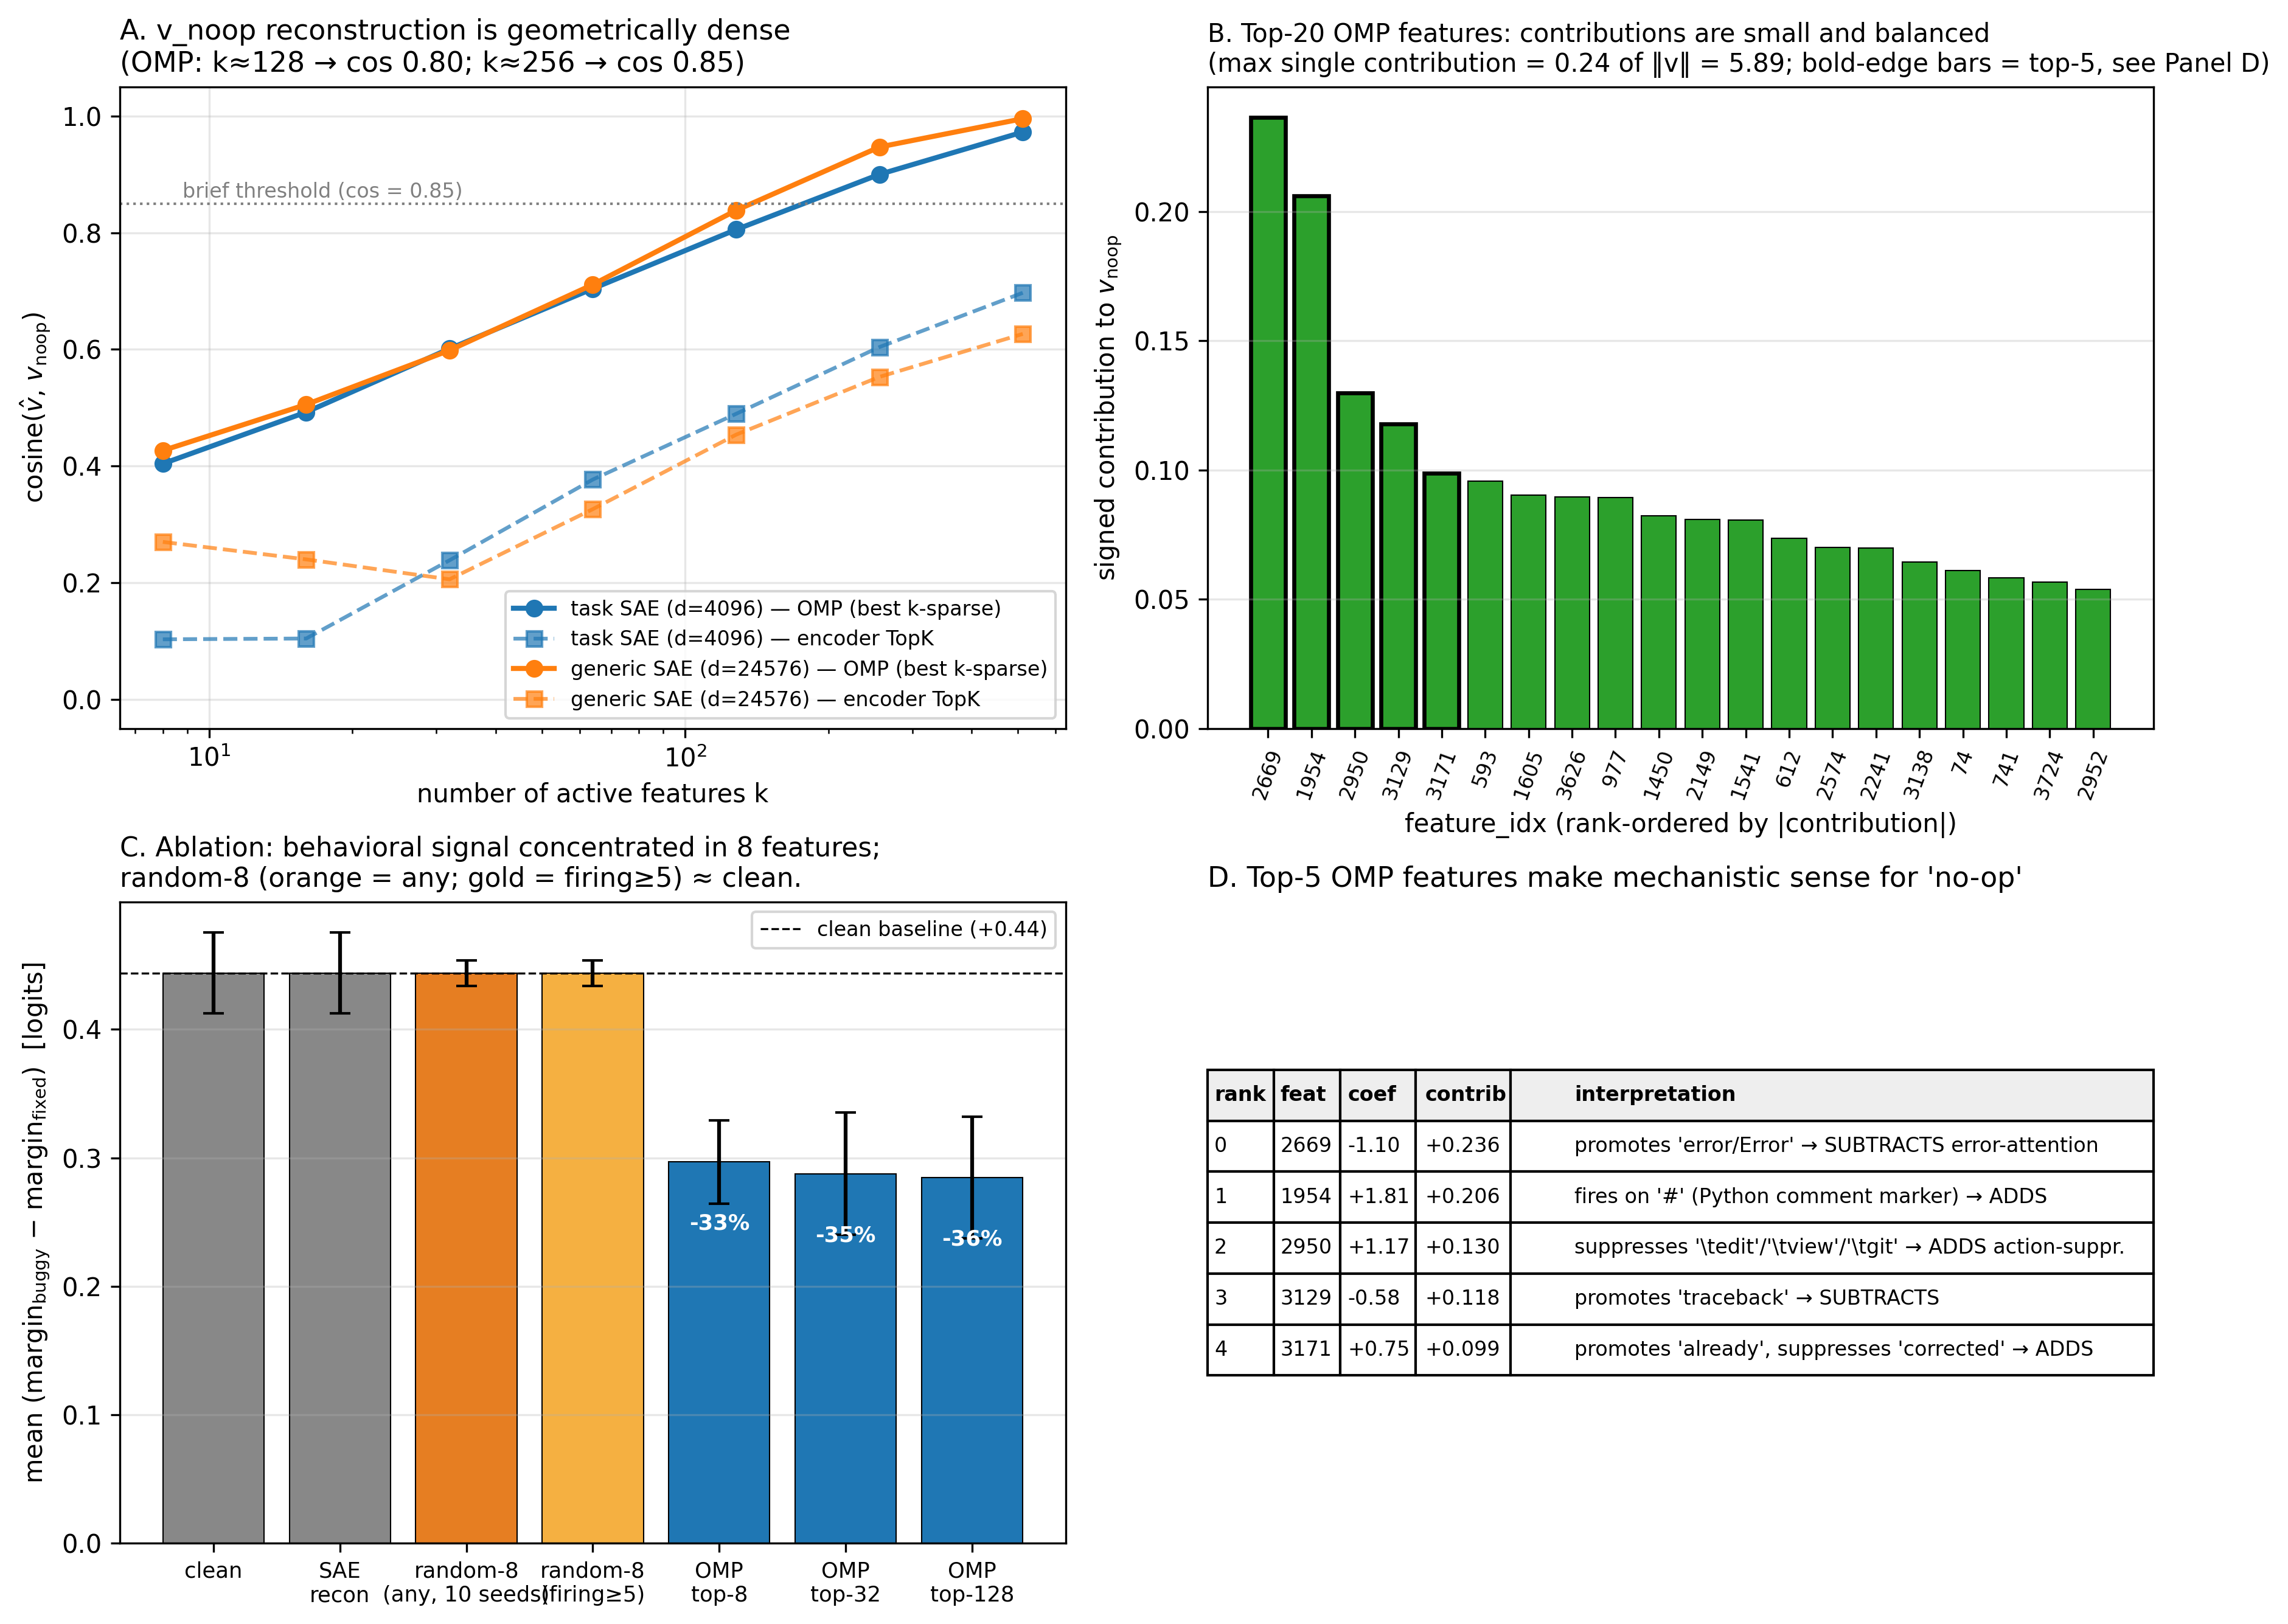
\includegraphics[width=0.98\linewidth,height=\textheight,keepaspectratio,alt={SAE feature decomposition of u\_\{\textbackslash rm tx\} (Qwen, L24 resid\_pre, task-distribution TopK SAE with d\_sae=4096, k=16, EV=0.976 over 1.23M positions).}]{figures/sae_decomposition.png}
\caption{SAE feature decomposition of \(u_{\rm tx}\) (Qwen, L24
resid\_pre, task-distribution TopK SAE with d\_sae=4096, k=16, EV=0.976
over 1.23M positions).}
\end{figure}

\begin{figure}
\centering
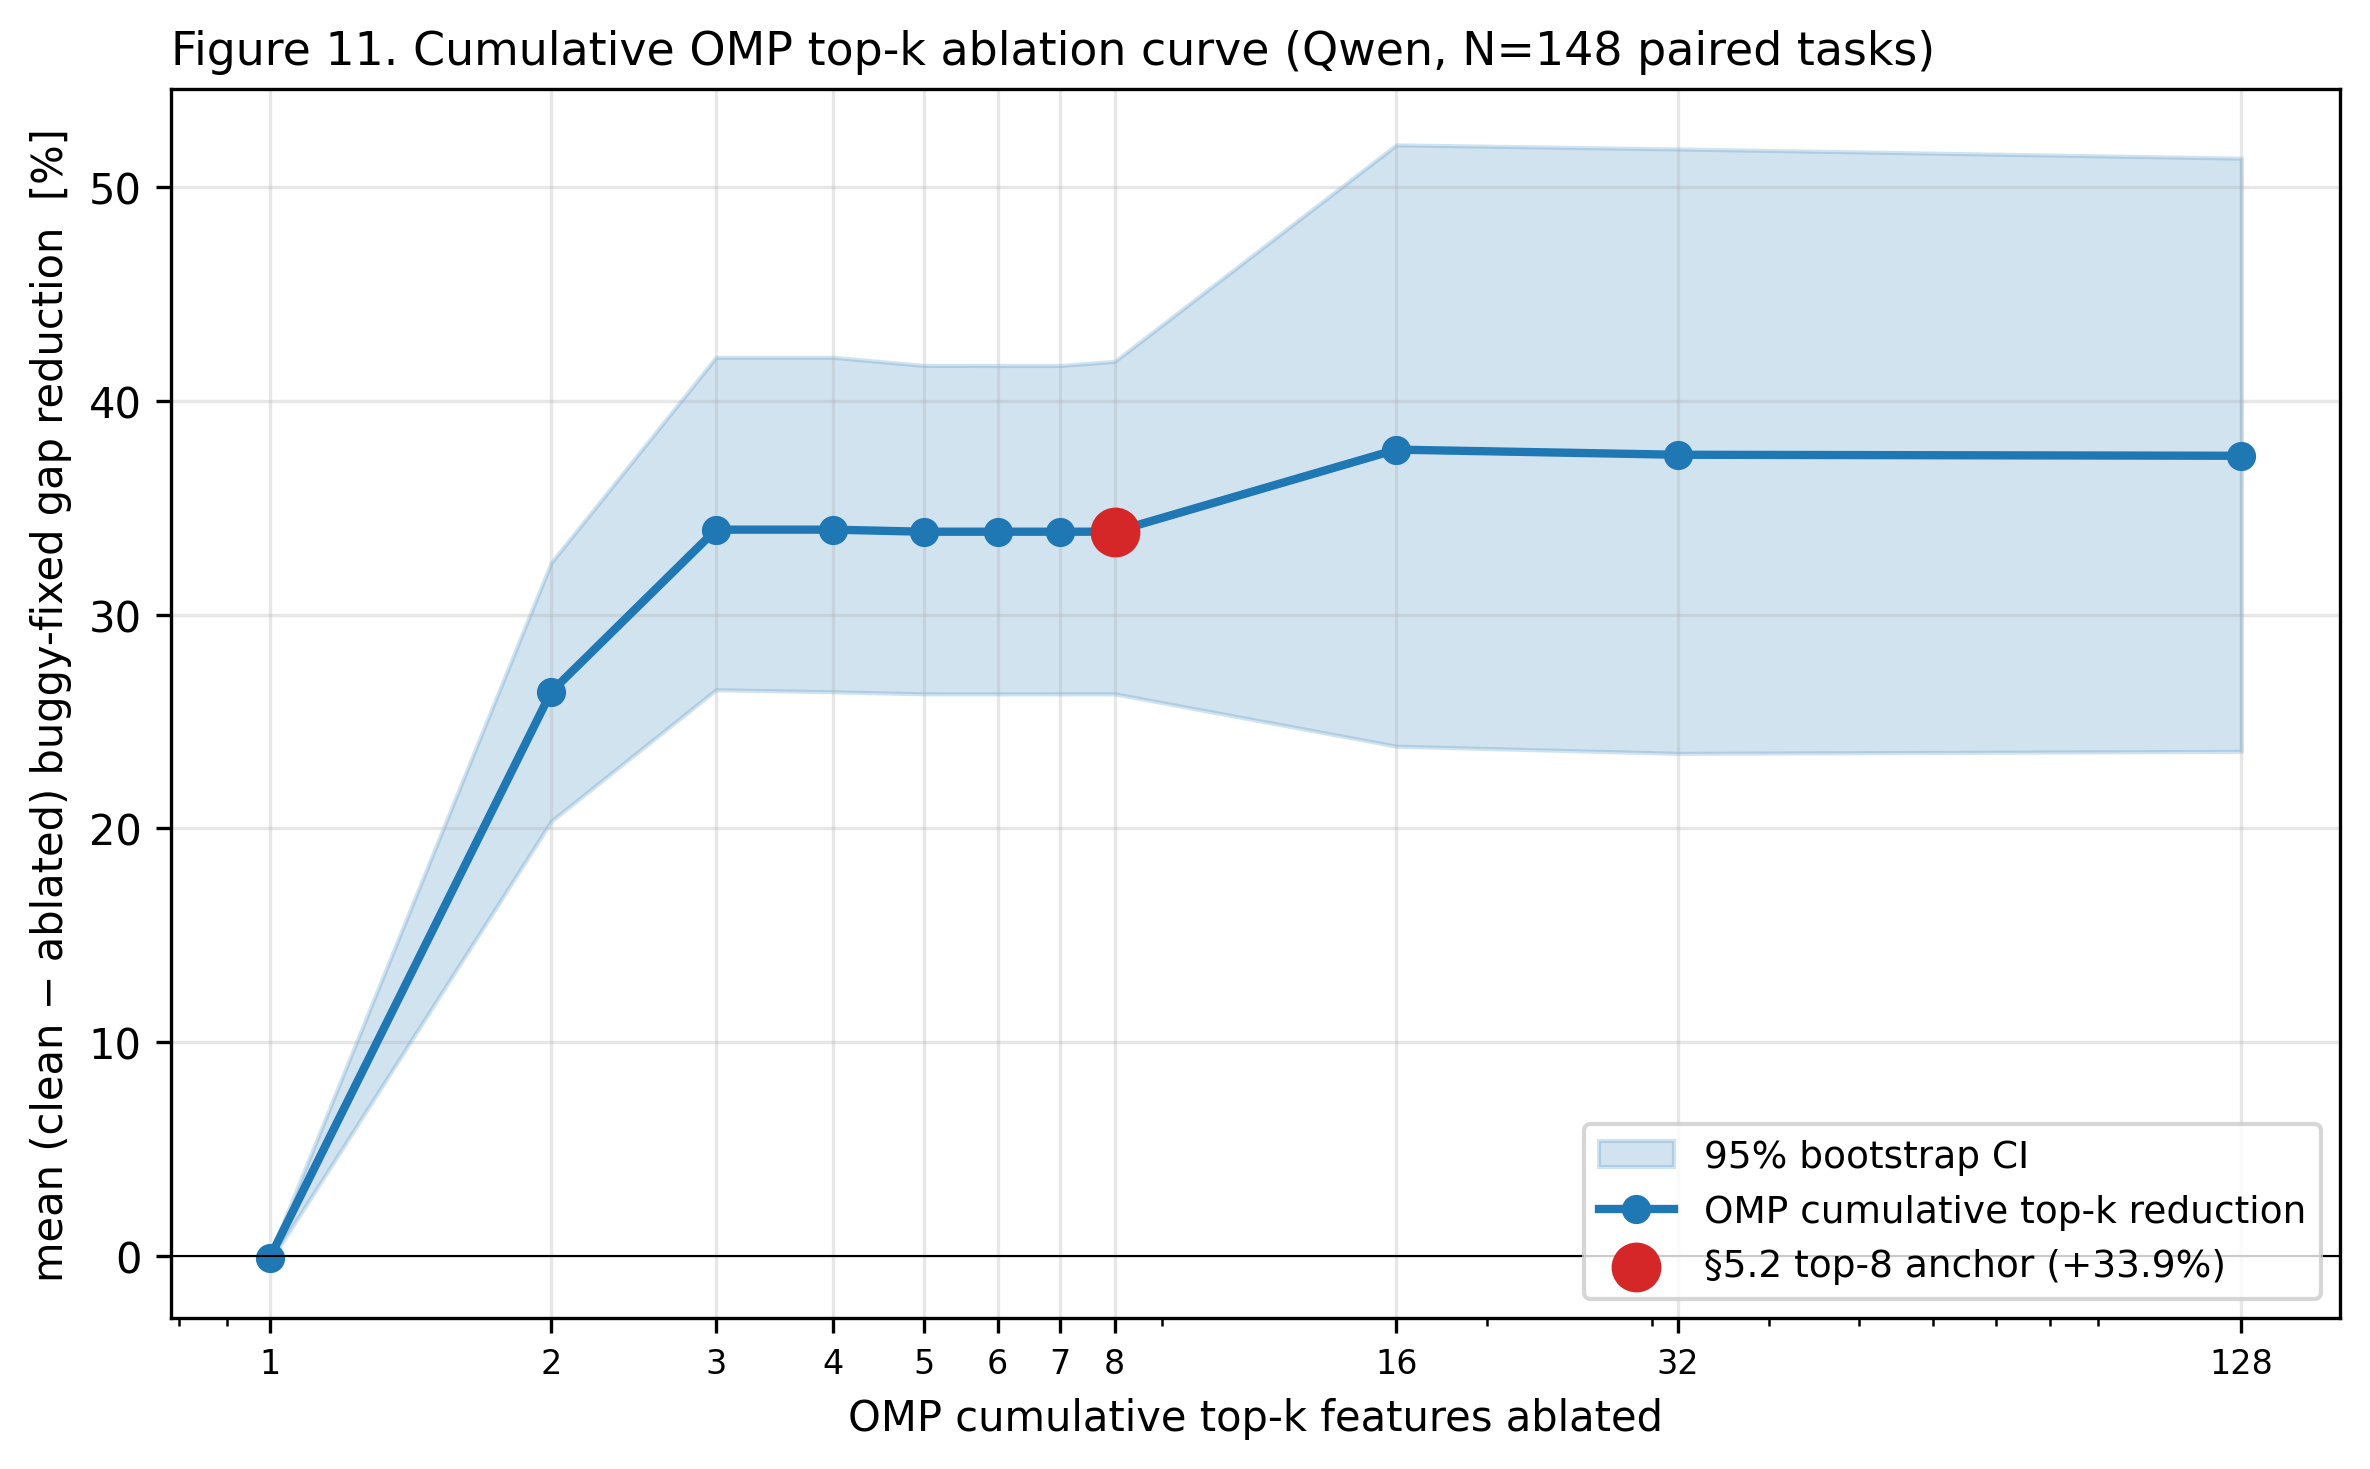
\includegraphics[width=0.85\linewidth,height=\textheight,keepaspectratio,alt={Cumulative OMP top-k ablation curve on Qwen (N=148 (task, variant) pairs from the 49-task toy substrate; 296 prompts with both buggy and fixed materialized).}]{figures/sae_topk_curve.png}
\caption{Cumulative OMP top-k ablation curve on Qwen (N=148 (task,
variant) pairs from the 49-task toy substrate; 296 prompts with both
\protect\texttt{buggy} and \protect\texttt{fixed} materialized).}
\end{figure}

\subsection{Cross-model SAE replication on CodeGemma (partial, uses the
20-task responsive-subset
direction)}\label{cross-model-sae-replication-on-codegemma-partial-uses-the-20-task-responsive-subset-direction}

\textbf{Direction used.} This exploratory CodeGemma SAE replication uses
the 20-task responsive-subset \texttt{v\_noop\_cg} (the direction used
in the \S{}4.2 steering plot, not the all-49 direction used for the \S{}5.1
monitor headline). The clean CodeGemma toy gap reported below (+2.589
logits) is the responsive-subset gap, not the all-49 gap of +1.347
reported in \S{}4.3. We retain the analysis as exploratory SAE evidence;
the all-49 CodeGemma SAE was not rerun. The 20-task subset is therefore
used in: (i) the \S{}4.2 steering plot, and (ii) this appendix; the \S{}5.1
monitor headline and \S{}4.3 cross-model table both use the all-49
direction.

We repeated the entire pipeline on CodeGemma-7B-it at L26/pos \ensuremath{-}1 using
the (responsive-subset) frozen v\_noop\_cg direction. The
\textbf{geometric} finding replicates; the \textbf{behavioral}
specificity finding does \textbf{not}.

\textbf{Setup.} We cached 1.20M positions of L26 resid\_pre over the
1282 task prompts and trained a TopK SAE with d\_sae = 8192, k = 48
(linear scaling from Qwen's d\_sae/d\_in = 2.67 ratio; we initially
trained at k = 24 matching Qwen's ratio but reached only EV = 0.75,
below our gate, so retrained at k = 48). The k = 48 SAE reached
\textbf{EV = 0.830} with 0.0\% dead features (in the {[}0.80, 0.85{]}
caveat band).

\textbf{Geometric result.} OMP k = 128 \ensuremath{\rightarrow} cos 0.677, k = 256 \ensuremath{\rightarrow} cos 0.779,
k = 1024 \ensuremath{\rightarrow} cos 0.969, same ``resist-sparsity'' character as Qwen.

\textbf{Behavioral result.} Running the per-feature-set ablation
pipeline on the 146 \texttt{(task,\ variant)} pairs that fit under the
2400-token cap (2 of 148 dropped for length):

{\def\LTcaptype{none} % do not increment counter
\begin{longtable}[]{@{}
  >{\raggedright\arraybackslash}p{(\linewidth - 8\tabcolsep) * \real{0.2877}}
  >{\raggedright\arraybackslash}p{(\linewidth - 8\tabcolsep) * \real{0.1370}}
  >{\raggedright\arraybackslash}p{(\linewidth - 8\tabcolsep) * \real{0.1507}}
  >{\raggedright\arraybackslash}p{(\linewidth - 8\tabcolsep) * \real{0.2603}}
  >{\raggedright\arraybackslash}p{(\linewidth - 8\tabcolsep) * \real{0.1644}}@{}}
\toprule\noalign{}
\begin{minipage}[b]{\linewidth}\raggedright
set
\end{minipage} & \begin{minipage}[b]{\linewidth}\raggedright
mean gap
\end{minipage} & \begin{minipage}[b]{\linewidth}\raggedright
reduction
\end{minipage} & \begin{minipage}[b]{\linewidth}\raggedright
95\% CI
\end{minipage} & \begin{minipage}[b]{\linewidth}\raggedright
Wilcoxon p
\end{minipage} \\
\midrule\noalign{}
\endhead
\bottomrule\noalign{}
\endlastfoot
clean (CodeGemma) & +2.589 & -- & -- & -- \\
sae\_recon (control) & +2.589 & 0.0\% & -- & -- \\
ablate OMP top-8 & +2.425 & \textbf{+6.4\%} & {[}\ensuremath{-}3.2\%, +16.4\%{]} &
\textbf{0.103} \\
ablate OMP top-32 & +3.178 & \ensuremath{-}22.7\% & {[}\ensuremath{-}34.4\%, \ensuremath{-}11.1\%{]} & 1.00 \\
ablate OMP top-128 & +2.972 & \ensuremath{-}14.8\% & {[}\ensuremath{-}25.4\%, \ensuremath{-}4.2\%{]} & 1.00 \\
\end{longtable}
}

On CodeGemma the OMP top-8 reduction is \textbf{+6.4\%} (CI includes
zero, p = 0.10, not significant), and the larger subsets \emph{increase}
the buggy-fixed gap by 15--23\%. The behavioral specificity claim that
holds on Qwen does not hold on CodeGemma. Three candidate explanations,
none isolable without further compute: (i) CodeGemma's SAE was weaker
(EV 0.830 vs Qwen 0.976); (ii) v\_noop\_cg was derived from a smaller
paired-task substrate (N = 20 vs 49 on Qwen); (iii) CodeGemma's L26 may
not encode the edit-vs-noop signal as a clean low-rank composition the
way Qwen's L24 does, even though both sites are at corresponding
relative depth and the monitor transfers cleanly to both.

\textbf{One CodeGemma feature is interpretable.} Feature 6974 (OMP rank
2, coef +1.05, contribution +0.170) promotes \texttt{passed},
\texttt{OK}, \texttt{pass}, a pass/fail-transcript feature (the
test-passing analog of Qwen's ``passing-test transcript'' feature), with
positive v\_noop\_cg contribution. The other top-5 features have lower
logit-lens interpretability (top promotions/suppressions are rare
non-English tokens), likely reflecting CodeGemma's larger vocabulary and
the more polysemantic features expected at 7B scale.

\begin{figure}
\centering
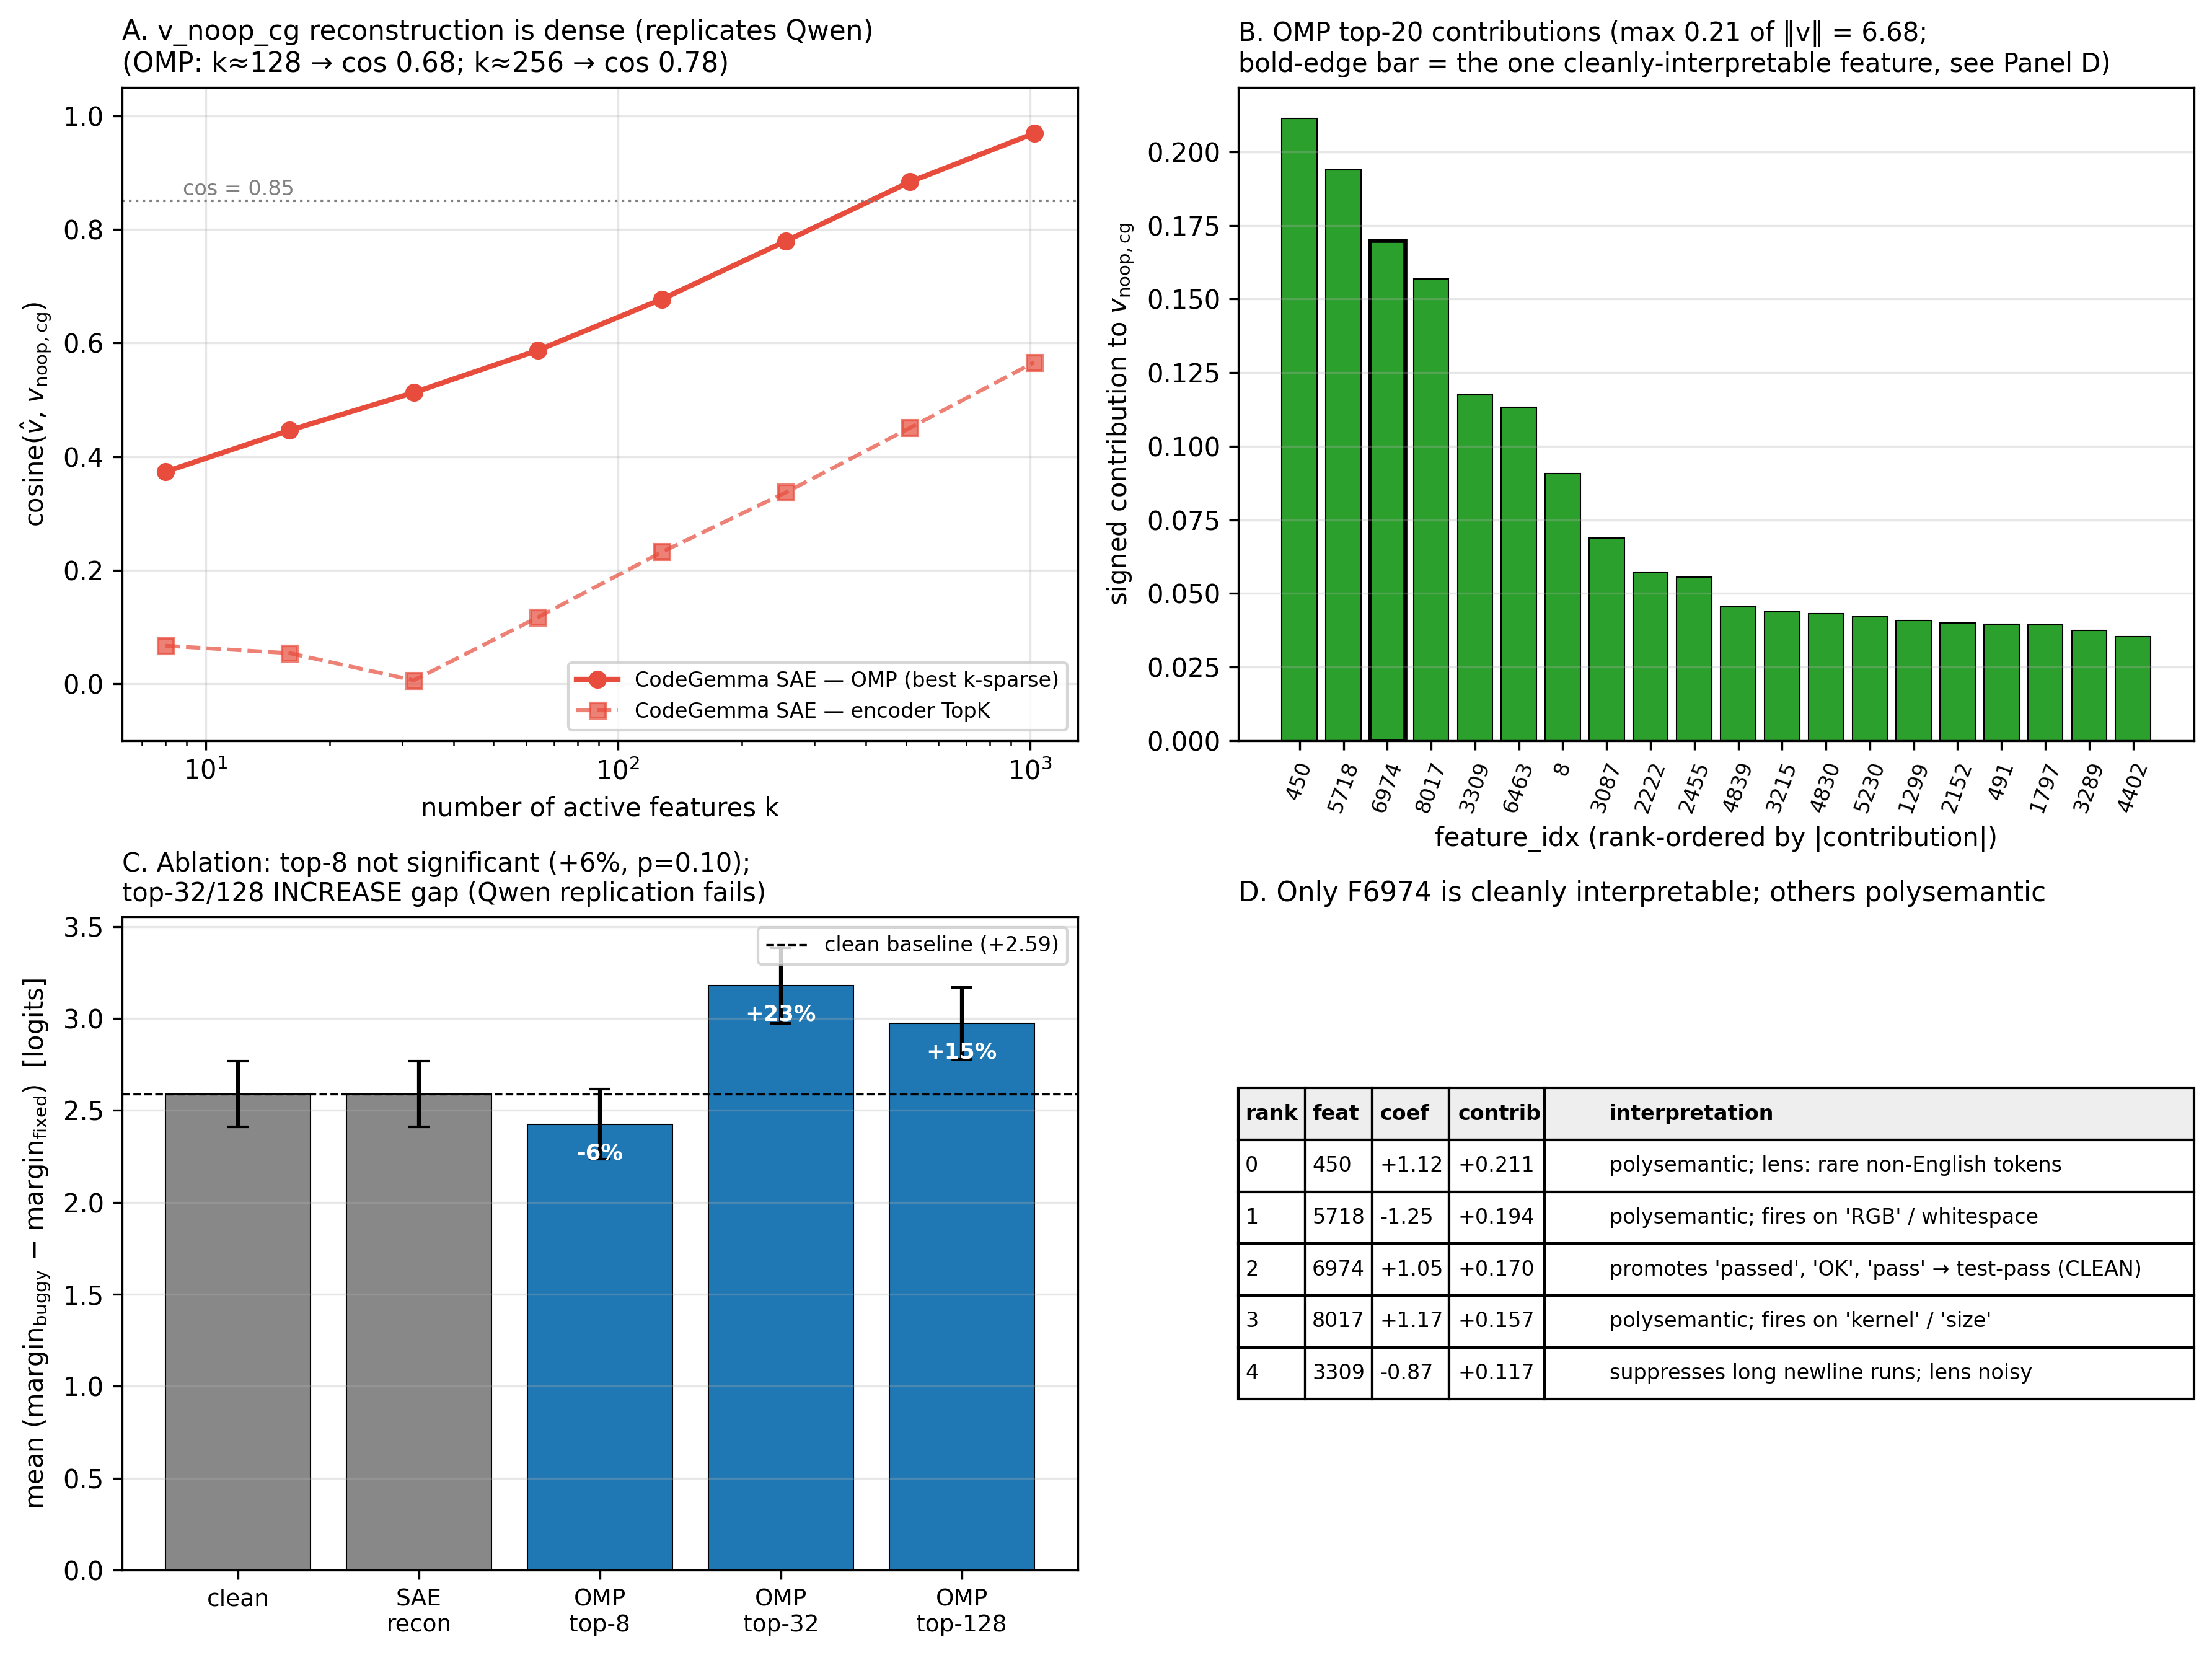
\includegraphics[width=0.98\linewidth,height=\textheight,keepaspectratio,alt={CodeGemma-7B SAE feature decomposition of v\_noop\_cg (L26 resid\_pre, task-distribution TopK SAE with d\_sae=8192, k=48, EV=0.830 over 1.20M positions).}]{figures/sae_decomposition_codegemma.png}
\caption{CodeGemma-7B SAE feature decomposition of v\_noop\_cg (L26
resid\_pre, task-distribution TopK SAE with d\_sae=8192, k=48, EV=0.830
over 1.20M positions).}
\end{figure}

\subsection{Seed=0 re-seed: geometric finding replicates; behavioral
sparse effect is qualitatively consistent but not
exact}\label{seed0-re-seed-geometric-finding-replicates-behavioral-sparse-effect-is-qualitatively-consistent-but-not-exact}

The headline SAE artifact for \S{}5.4 / H.1--H.5 pre-dates seed pinning
(see App. J.4); the specific feature indices (F1954, F2669, F2950,
F3129, F3171) are not bit-reproducible. We re-train the same
architecture under \texttt{-\/-seed\ 0} on the same 1.23M-position task
corpus and re-run OMP-k=128. The seed=0 cumulative-ablation re-run uses
a \textbf{broader 1096-prompt toy+SWE-derived evaluation set} (not the
296-prompt toy-only ablation set of H.2--H.4), so the comparison below
is \textbf{qualitative} rather than an exact replication of the H.2
296-prompt ablation curve. The new artifact:
\texttt{results/sae/qwen\_l24\_resid\_pre\_TASK\_d4096\_k16\_seed0.pt}
(EV = 0.962, l0 = 16.0, 0.0\% dead, 97 s training). Top-5 OMP features
by signed contribution: F1304, F3166, F639, F945, F3902, entirely
different indices, as expected for different SAE seeds.

\textbf{Geometric finding replicates.} \(u_{\rm tx}\) reconstruction
cosine at OMP-k=128: \textbf{0.812} (vs \textbf{0.806} in \S{}H.1), within
sampling noise. The ``dense in basis, OMP needs k \ensuremath{\approx} 128 for cos \ensuremath{\geq} 0.80''
qualitative claim is seed-robust.

\textbf{Behavioral-sparse finding: qualitatively consistent re-run.}
Cumulative OMP-top-k margin-gap reduction
(\texttt{scripts/ablation\_stats.py} on
\texttt{results/sae/ablate-distributed-seed0/}):

{\def\LTcaptype{none} % do not increment counter
\begin{longtable}[]{@{}
  >{\raggedleft\arraybackslash}p{(\linewidth - 6\tabcolsep) * \real{0.0714}}
  >{\raggedleft\arraybackslash}p{(\linewidth - 6\tabcolsep) * \real{0.2429}}
  >{\raggedleft\arraybackslash}p{(\linewidth - 6\tabcolsep) * \real{0.2000}}
  >{\raggedright\arraybackslash}p{(\linewidth - 6\tabcolsep) * \real{0.4857}}@{}}
\toprule\noalign{}
\begin{minipage}[b]{\linewidth}\raggedleft
k
\end{minipage} & \begin{minipage}[b]{\linewidth}\raggedleft
original (\S{}H.2)
\end{minipage} & \begin{minipage}[b]{\linewidth}\raggedleft
seed=0
\end{minipage} & \begin{minipage}[b]{\linewidth}\raggedright
comment
\end{minipage} \\
\midrule\noalign{}
\endhead
\bottomrule\noalign{}
\endlastfoot
1 & \ensuremath{-}0.10\% & \textbf{+25.7\%} & different feature ordering \\
2 & +26.4\% & \textbf{+30.3\%} & similar magnitude \\
3 & +34.0\% & +30.3\% & plateau onset matches \\
4 & +34.0\% & +30.2\% & plateau holds \\
5 & +33.9\% & +30.2\% & plateau holds \\
6 & +33.9\% & \textbf{\ensuremath{-}41.6\%} & inversion: gap WIDENS \\
7 & +33.9\% & \ensuremath{-}41.6\% & \\
8 & +33.9\% & \ensuremath{-}40.3\% & through k=8 plateau does NOT hold \\
16 & +37.7\% & +3.9\% & \\
32 & +37.5\% & +3.9\% & \\
128 & +37.4\% & \ensuremath{-}72.6\% & \\
\end{longtable}
}

What survives: at small k, OMP selection of features aligned with
\(u_{\rm tx}\) reduces the buggy-fixed margin gap by \textasciitilde30\%
(seed=0; was \textasciitilde34\% in the original artifact), with a sharp
non-linear onset between k=1 and k=2-5. The original-artifact statement
that the smallest tested subset reaching the plateau is three features
should therefore be read as artifact-specific rather than seed-robust:
under seed=0 the plateau is reached at \textbf{k=2} at +30.3\% (CI
{[}+26.8\%, +33.8\%{]}, Wilcoxon p \ensuremath{\approx} \(10^{-45}\)), and the plateau
width is much narrower (k=2-5 vs k=3-8). The +34\% number itself is a
seed-specific artifact; the qualitative ``small-k subset achieves
substantial gap reduction'' claim is robust, but the \textbf{precise
plateau magnitude and width depend on the SAE seed}.

What does \emph{not} survive: the ``plateau holds through k=8'' claim.
Under seed=0, ablating the OMP-top-6 through OMP-top-8 features
\emph{widens} the buggy-fixed gap (negative reduction). This is
consistent with the OMP procedure: features ranked 6-8 in seed=0 do not
have the same role as in the original artifact (different encoder learns
a different basis), and ablating them can shift the residual in the
opposite direction. The \S{}H.4 ``OMP-top-8 flips 80\% of argmaxes, nearly
all \texttt{grep\ \ensuremath{\rightarrow}\ edit}'' finding therefore cannot be read as a
stable property of the SAE basis; it is a property of the specific
(seed-unknown) artifact used in \S{}H.4 / \S{}5.4 / Fig. \ref{fig:sae}.

\textbf{How to read \S{}5.4 / \S{}H.2-H.5 in light of this.} The qualitative
findings (the contrast direction is dense in basis; a small OMP-selected
feature subset achieves a non-trivial, \textasciitilde30\%, gap
reduction; the reduction has a sharp non-linear onset between k=1 and
k=2-3) replicate. The quantitative headline numbers (+34.0\% margin
reduction at OMP-k=3, 80.1\% argmax flip at OMP-k=8, the specific
F-indices in \S{}H.5) \textbf{do not replicate exactly} under a re-seeded
SAE and should be read as artifact-specific. The semantic logit-lens
interpretations in \S{}H.5 (error / traceback / already) similarly depend
on the artifact; in light of \S{}5.2 the right interpretation is anyway
pass/fail-transcript features, not ``no-op circuit elements.''

Outputs:
\texttt{results/sae/v\_noop\_features\_DISTRIBUTED\_seed0.json},
\texttt{results/}\allowbreak\texttt{sae/}\allowbreak\texttt{ablate-}\allowbreak\texttt{distributed-}\allowbreak\texttt{seed0/}\allowbreak\texttt{ablation\_results.json},
\texttt{results/}\allowbreak\texttt{sae/}\allowbreak\texttt{ablate-}\allowbreak\texttt{distributed-}\allowbreak\texttt{seed0/}\allowbreak\texttt{ablation\_stats.json}.

\section{In-context attribution within the cached last-32-token
window}\label{in-context-attribution-within-the-cached-last-32-token-window}

On the existing toy cache the residual stream is stored only for the
\textbf{last 32 token positions} of each prompt. Across all 49 paired
toys the last-32-token sequence is identical: 13 tokens of canonical
question text, 12 tokens of chat-template close, and 7 tokens of
\texttt{Action:} suffix. Any buggy-vs-fixed differential in the L24
resid\_pre projection onto \(u_{\rm tx}\) at a given offset is therefore
\textbf{purely attentional information flow} from the earlier (varying)
test-output and code content.

\textbf{Per-offset projection} (per-offset paired Wilcoxon p \textless{}
\(10^{-10}\) at every position):

{\def\LTcaptype{none} % do not increment counter
\begin{longtable}[]{@{}
  >{\raggedright\arraybackslash}p{(\linewidth - 8\tabcolsep) * \real{0.3647}}
  >{\raggedright\arraybackslash}p{(\linewidth - 8\tabcolsep) * \real{0.1647}}
  >{\raggedleft\arraybackslash}p{(\linewidth - 8\tabcolsep) * \real{0.1529}}
  >{\raggedleft\arraybackslash}p{(\linewidth - 8\tabcolsep) * \real{0.1529}}
  >{\raggedleft\arraybackslash}p{(\linewidth - 8\tabcolsep) * \real{0.1647}}@{}}
\toprule\noalign{}
\begin{minipage}[b]{\linewidth}\raggedright
section
\end{minipage} & \begin{minipage}[b]{\linewidth}\raggedright
offset range
\end{minipage} & \begin{minipage}[b]{\linewidth}\raggedleft
mean(buggy)
\end{minipage} & \begin{minipage}[b]{\linewidth}\raggedleft
mean(fixed)
\end{minipage} & \begin{minipage}[b]{\linewidth}\raggedleft
differential
\end{minipage} \\
\midrule\noalign{}
\endhead
\bottomrule\noalign{}
\endlastfoot
question text & {[}\ensuremath{-}31, \ensuremath{-}19{]} & +2.25 & +3.24 & \textbf{+0.99} \\
chat-template close & {[}\ensuremath{-}18, \ensuremath{-}7{]} & +2.36 & +3.10 & \textbf{+0.74} \\
\texttt{Action:} suffix & {[}\ensuremath{-}6, 0{]} & \ensuremath{-}0.94 & +2.40 &
\textbf{+3.34} \\
\end{longtable}
}

The differential grows monotonically as we approach the Action position,
from \ensuremath{\approx}+1 logit-unit at offset \ensuremath{-}31 to \textbf{+5.9 at offset 0}. The
per-token Action: suffix differential (+3.34) is \textbf{3.4\ensuremath{\times} stronger}
than the question-text section (+0.99). The \(u_{\rm tx}\) signal is
present throughout the prompt tail but \textbf{crystallizes sharply over
the final seven positions}.

\begin{figure}
\centering
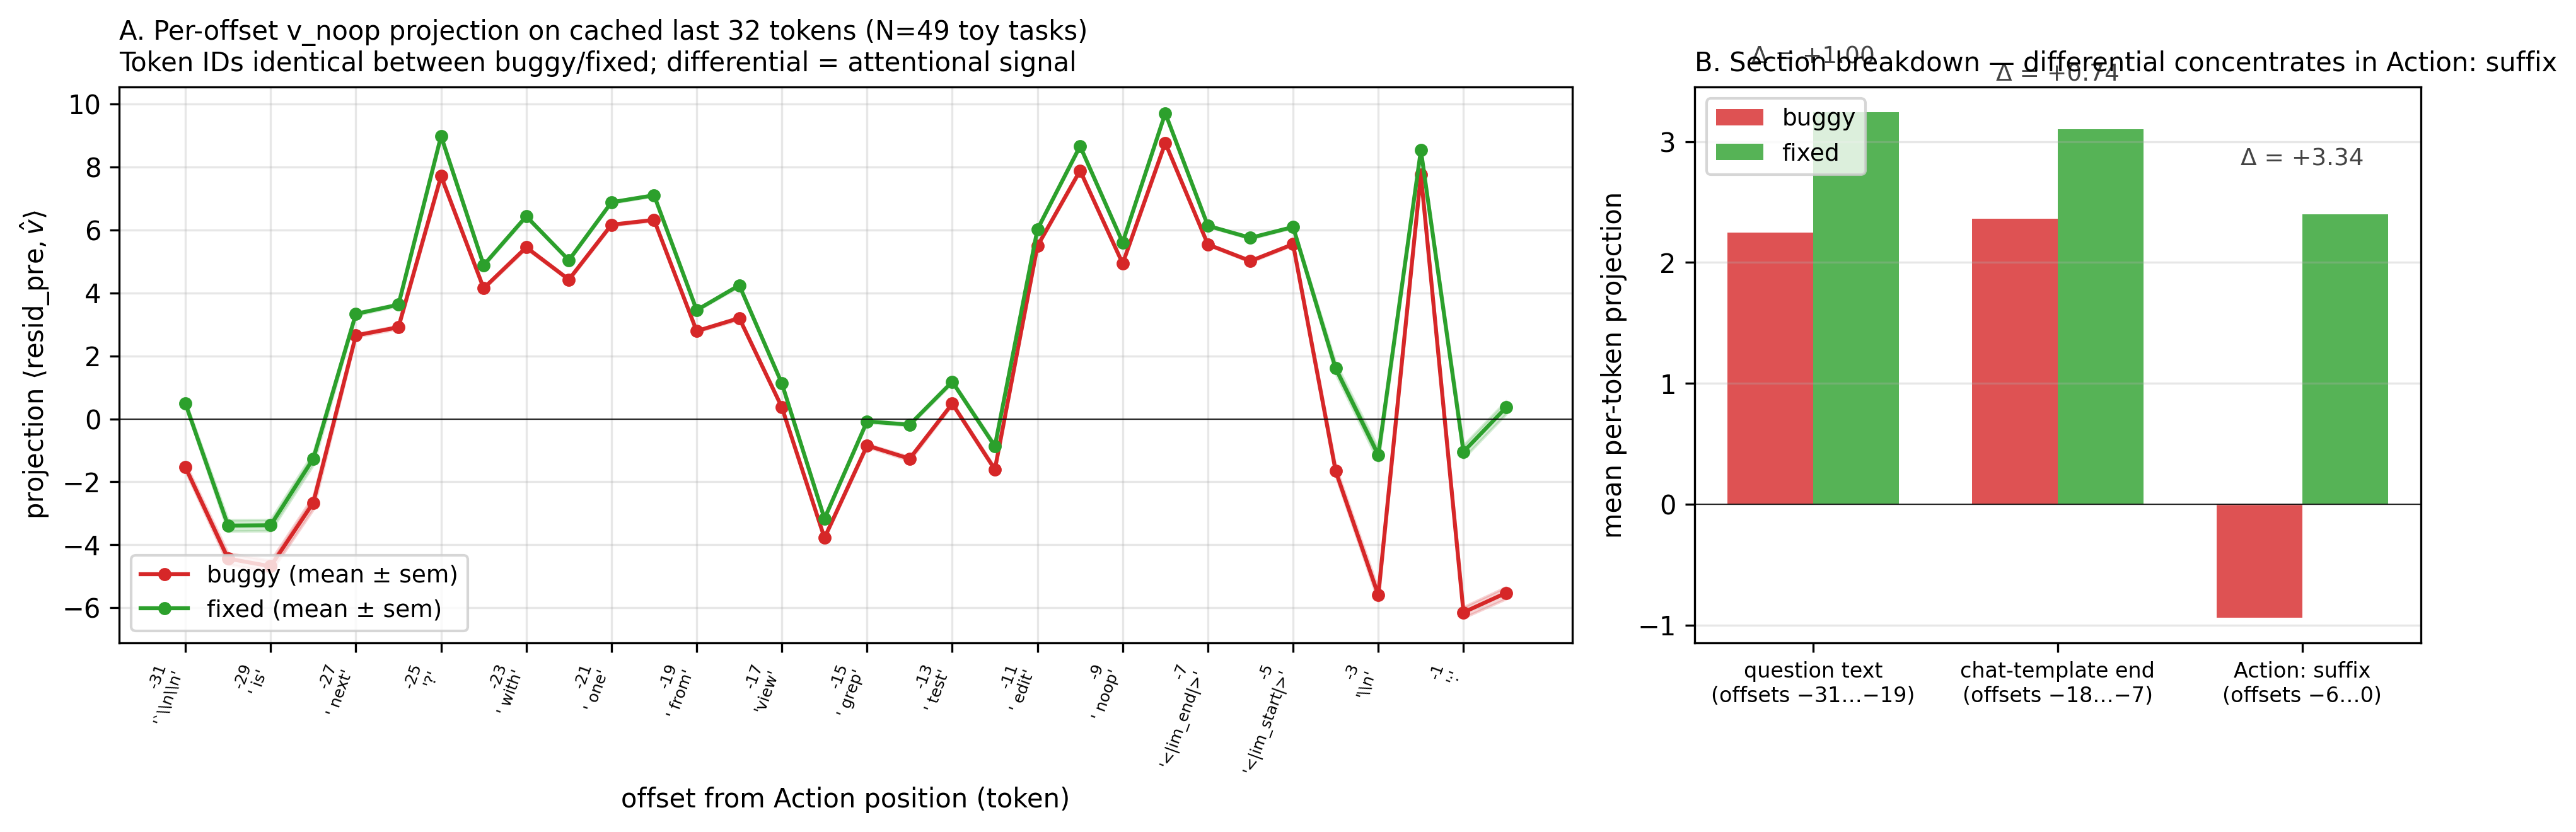
\includegraphics[width=0.98\linewidth,height=\textheight,keepaspectratio,alt={In-context attribution of u\_\{\textbackslash rm tx\} on Qwen toy substrate (N=49 paired tasks).}]{figures/incontext_attribution.png}
\caption{In-context attribution of \(u_{\rm tx}\) on Qwen toy substrate
(N=49 paired tasks).}
\end{figure}

\section{Reproduction}\label{reproduction}

\subsection{Bootstrap}\label{bootstrap}

The source repository and small analysis artifacts are public; the large
activation caches are archived at the Hugging Face dataset listed below.

\begin{Shaded}
\begin{Highlighting}[]
\FunctionTok{git}\NormalTok{ clone https://github.com/faizancodes/no{-}op{-}circuit{-}paper.git}
\BuiltInTok{cd}\NormalTok{ no{-}op{-}circuit{-}paper }\KeywordTok{\&\&} \ExtensionTok{python} \AttributeTok{{-}m}\NormalTok{ venv .venv }\KeywordTok{\&\&} \BuiltInTok{source}\NormalTok{ .venv/bin/activate}
\ExtensionTok{pip}\NormalTok{ install }\AttributeTok{{-}e} \StringTok{".[analysis]"}
\FunctionTok{cp}\NormalTok{ .env.example .env }\CommentTok{\# fill in MODAL\_TOKEN\_ID, MODAL\_TOKEN\_SECRET,}
 \CommentTok{\# HF\_TOKEN, OPENROUTER\_API\_KEY}
\end{Highlighting}
\end{Shaded}

\subsection{Cost table}\label{cost-table}

Tracked Modal compute before the final consistency-pass experiments was
approximately \textbf{\$17} (the original \textasciitilde\$8.91; plus
\textasciitilde\$4 of paraphrase-cache jobs across three models for App.
G.12; plus \textasciitilde\$4 of later server-side scoring jobs for the
temporal-separation control (App. G.15, Qwen) and the cross-model
contradictory-transcript control (App. G.16, CodeGemma + DeepSeek). The
cross-format layer/position sweeps and the all-49 CodeGemma recompute
are pure local computation on previously cached residuals, \$0 added
Modal cost.) OpenRouter (LLM-generated tasks + flaky transcripts):
\textbf{\textasciitilde\$6}; approximate total cloud cost
\textbf{\textasciitilde\$23} (approximate cloud-cost figures, not an
audited bill; the later consistency-pass jobs below were not separately
tracked, so the true total is slightly higher). The SWE-derived
peak-cell patching job (Qwen, N=200, three cells; \S{}4.1), the toy
discrete five-action patching job (Qwen, N=49; \S{}5.6), and the
cross-model five-action follow-ups (CodeGemma-7B on A100, N=49;
DeepSeek-Coder-1.3B single-token, N=49; \S{}5.6) were added after the
earlier cost accounting and were not separately tracked. The CodeGemma
vs \S{}4.3 consistency audit
(\texttt{scripts/audit\_patching\_consistency.py}) is pure local CPU
computation, \$0 added Modal cost. Phase-by-phase breakdown in the
project repository (long-form per-experiment cost table; this appendix
collapses it to the headline). The action-menu controls (action-order /
binary / abstract-label / letter-only on Qwen; action-order / binary on
CodeGemma (A100) and DeepSeek; the DeepSeek single-token rerun) and the
noisy-transcript monitor run are small first-token-scoring jobs added
later; their cost was not separately tracked but is on the order of a
few dollars total. The five-action steering decomposition, the BoW /
paraphrase baselines, and the tokenization audit are pure local
computation (\$0 added Modal cost).

\subsection{Entry points}\label{entry-points}

All Modal entry points expose \texttt{-\/-model}, \texttt{-\/-layer},
and \texttt{-\/-run-id} flags. The three core jobs:

\begin{Shaded}
\begin{Highlighting}[]
\CommentTok{\# Cache residual streams for all 49 tasks \ensuremath{\times} variants \ensuremath{\times} \{buggy, fixed\}}
\ExtensionTok{modal}\NormalTok{ run }\AttributeTok{{-}m}\NormalTok{ modal\_app.cache\_dataset }\AttributeTok{{-}{-}model} \OperatorTok{\textless{}}\NormalTok{hf{-}slug}\OperatorTok{\textgreater{}} \DataTypeTok{\textbackslash{}}
 \AttributeTok{{-}{-}variants}\NormalTok{ issue\_only,code,code\_tests}

\CommentTok{\# Bidirectional activation patching (peak{-}cell heatmaps)}
\ExtensionTok{modal}\NormalTok{ run }\AttributeTok{{-}m}\NormalTok{ modal\_app.patch\_dataset }\AttributeTok{{-}{-}model} \OperatorTok{\textless{}}\NormalTok{hf{-}slug}\OperatorTok{\textgreater{}} \DataTypeTok{\textbackslash{}}
 \AttributeTok{{-}{-}variant}\NormalTok{ code\_tests }\AttributeTok{{-}{-}max{-}suffix}\NormalTok{ 2 }\AttributeTok{{-}{-}layer{-}step}\NormalTok{ 2 }\AttributeTok{{-}{-}bidirectional}

\CommentTok{\# Single{-}direction steering (computes the raw contrast vector, sweeps \ensuremath{\alpha})}
\ExtensionTok{modal}\NormalTok{ run }\AttributeTok{{-}m}\NormalTok{ modal\_app.steer\_dataset }\AttributeTok{{-}{-}model} \OperatorTok{\textless{}}\NormalTok{hf{-}slug}\OperatorTok{\textgreater{}} \DataTypeTok{\textbackslash{}}
 \AttributeTok{{-}{-}cache{-}dir}\NormalTok{ results/cache{-}}\OperatorTok{\textless{}}\NormalTok{RUN\_ID}\OperatorTok{\textgreater{}} \DataTypeTok{\textbackslash{}}
 \AttributeTok{{-}{-}variant}\NormalTok{ code\_tests }\AttributeTok{{-}{-}layer} \OperatorTok{\textless{}}\NormalTok{peak}\OperatorTok{\textgreater{}}\NormalTok{ {-}{-}position }\AttributeTok{{-}1}
\end{Highlighting}
\end{Shaded}

Local analysis scripts (\texttt{scripts/run\_monitor\_real.py},
\texttt{scripts/ablation\_stats.py},
\texttt{scripts/codegemma\_per\_repo\_calibration.py},
\texttt{scripts/incontext\_attribution.py},
\texttt{paper/figures/render\_all.py}) regenerate all monitor metrics
and figures from the cached \texttt{.pt} files and the trained v\_noop /
SAE artifacts under \texttt{results/}.

The consistency-pass experiments add these entry points:
\texttt{scripts/check\_action\_tokenization.py} (tokenization audit);
\texttt{modal\_app/action\_order\_control.py} +
\texttt{scripts/run\_action\_order\_control.py} +
\texttt{scripts/analyze\_action\_order\_control.py} (action-menu /
position-balance controls, including the DeepSeek single-token rerun via
\texttt{-\/-experiment\ action\_order\_custom\ -\/-action-words\ view,find,test,edit,done});
\texttt{scripts/analyze\_five\_action\_decomp.py} (five-action steering
decomposition, no GPU); \texttt{modal\_app/noisy\_monitor.py} +
\texttt{scripts/analyze\_noisy\_monitor.py} (noisy-transcript monitor vs
regex vs bag-of-words); \texttt{scripts/paraphrase\_baselines.py}
(keyword / BoW paraphrase baselines, no GPU); and
\texttt{modal\_app/swe\_peak\_patching.py} +
\texttt{scripts/analyze\_swe\_peak\_patching.py} (Qwen SWE-derived
peak-cell causal patching at L24/pos \ensuremath{-}1 with L12/pos \ensuremath{-}1 and L24/pos \ensuremath{-}8
controls, all five action logits; doubles as a discrete five-action
patching decomposition on the 49 toys via
\texttt{-\/-tasks\ toy\ -\/-output-dir\ results/five\_action\_decomp},
including A100 dispatch via \texttt{-\/-gpu\ a100} for CodeGemma-7B and
a custom single-token vocabulary via
\texttt{-\/-action-words\ view,find,test,edit,done\ -\/-abstain-word\ done}
for the DeepSeek single-token follow-up at L22/pos \ensuremath{-}1). Outputs:
\texttt{results/swe\_peak\_patching/qwen\_swe\_peak\_patch\_\{scores,summary\}.json};
\texttt{results/five\_action\_decomp/qwen\_patching\_five\_action\_\{scores,summary\}.json}
(Qwen);
\texttt{results/five\_action\_decomp/deepseek\_swe\_peak\_patch\_\{scores,summary\}\_toy\_single\_token.json}
(DeepSeek single-token follow-up); and
\texttt{results/five\_action\_decomp/codegemma\_swe\_peak\_patch\_\{scores,summary\}\_toy.json}
(CodeGemma, pending consistency reconciliation with the \S{}4.3 May-2026
artifact \texttt{results/patch-codegemma\_7b\_it-20260516T031403Z/}; see
\texttt{scripts/audit\_patching\_consistency.py} and
\texttt{results/consistency\_audit/patching\_consistency\_audit.json}
for the audit output).

The \textbf{held-out paraphrase robustness} test (App. G.17) uses
\texttt{scripts/heldout\_paraphrase\_robustness.py}:
\texttt{-\/-self-test} checks template-vocabulary disjointness on CPU;
\texttt{-\/-run} renders the 499 SWE-derived paired prompts under each
template family and scores the model's frozen toy-trained direction at
its reported cell via \texttt{modal\_app.noisy\_monitor.score\_monitor}
(\texttt{score\_monitor\_a100} for the 7B CodeGemma);
\texttt{-\/-reanalyze} recomputes all per-template AUC/AP, the
train\ensuremath{\rightarrow}held-out BoW prediction spread, the score gaps, and the
lowercase/\texttt{{[}a-z{]}+}-tokenization/stopword-stripped
vocabulary-overlap report from the cached scores on CPU (no new
forwards). It is run cross-model at each model's \S{}4.3 reported cell with
\textbf{no post-hoc layer/position search}, via the \texttt{-\/-model},
\texttt{-\/-site-layer}, \texttt{-\/-direction-path},
\texttt{-\/-output-prefix}, and \texttt{-\/-gpu} flags. The cells and
frozen toy-trained directions are: Qwen L24/pos \ensuremath{-}1
(\texttt{results/}\allowbreak\texttt{steer-20260516T021522Z/v\_noop.pt});
CodeGemma L26/pos \ensuremath{-}1 (all-49 direction
\texttt{results/}\allowbreak\texttt{v\_noop\_codegemma\_all49.pt},
scored on A100); DeepSeek L22/pos \ensuremath{-}1
(\texttt{results/}\allowbreak\texttt{steer-deepseek-coder-13b-instruct-}\allowbreak\texttt{20260517T012848Z/v\_noop.pt};
legacy artifact path name, model is DeepSeek-Coder-1.3B). Outputs
\texttt{results/}\allowbreak\texttt{heldout\_paraphrase\_robustness/}\allowbreak\texttt{\{qwen,codegemma,deepseek\}\_\{summary,scores\}.json};
each summary JSON records the model, site, direction artifact, exact
preprocessing, and vocabulary-overlap report. The text baselines
(literal-\texttt{FAILED}, train-vocabulary keyword, train\ensuremath{\rightarrow}held-out BoW)
are model-independent and are fit only on train-template text.

\textbf{\S{}5.6 five-action decomposition, renderer reconciliation (detail
moved from \S{}5.6).} The \S{}5.6 table is a five-action \emph{sanity check}
under the current decomposition renderer
(\texttt{modal\_app/swe\_peak\_patching.py}), not a re-estimate of the
\S{}4.1/\S{}4.3 causal-localization numbers. The \S{}4.1/\S{}4.3 estimates (Qwen toy
clean B\ensuremath{-}F gap +0.659, F\ensuremath{\rightarrow}B +0.648, 43-task bidirectional +0.69/+0.64)
come from the original paper renderer; that toy \texttt{code\_tests}
\emph{patch} artifact is not available locally (only the \texttt{code}
negative-control variant is) and is not in the HF archive
\texttt{faizancodes/no-op-circuit-caches} (which holds the SWE-derived
residual caches, not the toy patch grid), so a per-task prompt-hash /
margin reconciliation could not be completed. The current-renderer Qwen
F\ensuremath{\rightarrow}B shift (+0.625) is close to \S{}4.1's +0.648, but the current-renderer
clean B\ensuremath{-}F gap (+0.532) is lower than \S{}4.1's +0.659, the same
fixed-condition renderer-drift direction found for CodeGemma. We
therefore keep the \S{}4.1/\S{}4.3 numbers as the localization estimates and
present \S{}5.6 only as a sanity check (reconciliation:
\texttt{scripts/}\allowbreak\texttt{reconcile\_qwen\_five\_action.py}
and
\texttt{scripts/}\allowbreak\texttt{audit\_qwen\_five\_action\_consistency.py};
outputs
\texttt{results/}\allowbreak\texttt{consistency\_audit/}\allowbreak\texttt{qwen\_five\_action\_reconciliation.\{json,md\}}
and \texttt{qwen\_five\_action\_consistency\_audit.json}). For
CodeGemma, the audit
(\texttt{scripts/}\allowbreak\texttt{audit\_patching\_consistency.py})
finds matching action token IDs and task IDs but a systematic
newer-renderer fixed-condition drift (new \ensuremath{-} old buggy diff mean +0.08,
median 0.0; fixed diff mean \ensuremath{-}1.31, median \ensuremath{-}2.0; new B\ensuremath{-}F gap mean +2.73
vs old +1.35); this is a renderer-comparability issue for the newer
five-action decomposition, not a correction to the \S{}4.3 reported-cell
result, so CodeGemma is omitted from the \S{}5.6 table while its
qualitative \texttt{noop}-never-induced result (0/49 clean and patched)
stands.

\subsection{Reproducibility: pinned random
seeds}\label{reproducibility-pinned-random-seeds}

All scripts and Modal entry points accept \texttt{-\/-seed} (default
\texttt{0}) and seed \texttt{torch}, \texttt{torch.cuda},
\texttt{numpy}, and \texttt{random} from a single source.
\texttt{torch.use\_deterministic\_algorithms(True,\ warn\_only=True)} is
enabled so non-deterministic CUDA kernels emit warnings instead of
silently diverging. The pinned scripts:

{\def\LTcaptype{none} % do not increment counter
\begin{longtable}[]{@{}
  >{\raggedright\arraybackslash}p{(\linewidth - 2\tabcolsep) * \real{0.6625}}
  >{\raggedright\arraybackslash}p{(\linewidth - 2\tabcolsep) * \real{0.3375}}@{}}
\toprule\noalign{}
\begin{minipage}[b]{\linewidth}\raggedright
script
\end{minipage} & \begin{minipage}[b]{\linewidth}\raggedright
seeded via
\end{minipage} \\
\midrule\noalign{}
\endhead
\bottomrule\noalign{}
\endlastfoot
\texttt{modal\_app/train\_sae.py} & \texttt{-\/-seed} \\
\texttt{modal\_app/ablate\_sae\_features.py} & \texttt{-\/-seed} \\
\texttt{modal\_app/ablate\_random\_features.py} & \texttt{-\/-base-seed}
(per-draw) \\
\texttt{scripts/train\_probes.py} & \texttt{-\/-seed} \\
\texttt{scripts/run\_monitor\_real.py} & \texttt{-\/-seed} \\
\texttt{scripts/ablation\_stats.py} & \texttt{-\/-seed}
(pre-existing) \\
\texttt{scripts/compute\_auc\_cis.py} (B4) & \texttt{-\/-seed} \\
\texttt{scripts/adversarial\_v\_noop\_baselines.py} (B6) &
\texttt{-\/-seed} \\
\texttt{modal\_app/swe\_peak\_patching.py} & \texttt{-\/-seed} (subset
selection) \\
\end{longtable}
}

\textbf{Caveat (the headline SAE artifact, now characterized by H.7).}
The Qwen TopK SAE referenced in \S{}5.4 / Appendix H.5,
\texttt{sae/qwen\_l24\_resid\_pre\_TASK\_d4096\_k16.pt}, EV 0.976, was
trained \textbf{before} seed pinning was added. App. H.7 now reports a
seed=0 re-train of the same architecture on the same corpus and compares
the results directly. The \textbf{geometric finding} replicates
(\(u_{\rm tx}\) reconstruction cosine at OMP-k=128 is 0.812 vs 0.806).
The \textbf{behavioral-sparse finding} \emph{partially} replicates: a
small OMP-selected feature subset still achieves \textasciitilde30\%
margin-gap reduction with a sharp non-linear onset between k=1 and k=2,
but the \textbf{precise +34.0\% plateau magnitude and through-k=8
plateau width do NOT replicate} (seed=0 plateau is +30.3\% at k=2-5,
with the plateau ending at k=5 instead of holding through k=8). The
80\%-argmax-flip number from H.4 is therefore artifact-specific rather
than seed-robust. The current \texttt{train\_sae.py} is seed-pinned; the
seed-unknown artifact is bundled with the code release only to preserve
the literal F-indices in App. H.5 (which are themselves
artifact-specific; the seed=0 top-5 indices are entirely different).

\subsection{Activation caches (HuggingFace
dataset)}\label{activation-caches-huggingface-dataset}

The residual-stream activation caches that the monitor, control, and
sweep analyses run on (\textasciitilde66 GB of per-(task, variant,
condition) \texttt{.pt} tensors across the three models) are archived as
a public HuggingFace dataset:
\textbf{\texttt{huggingface.co/datasets/faizancodes/no-op-circuit-caches}}.
The dataset card documents the cache contents, its limitations as a
non-source release, and the prompt-derived metadata caveats
(e.g.~last-token text / token ids that may contain short oracle-window
fragments). The small consistency-pass artifacts ship in the repo under
\texttt{results/}: \texttt{action\_order\_control/},
\texttt{five\_action\_decomp/}, \texttt{noisy\_monitor/},
\texttt{paraphrase\_baselines/}, and \texttt{tokenization/}. The small
artifacts the analyses also need, the per-model frozen \texttt{v\_noop}
directions (\texttt{results/steer-*/v\_noop.pt},
\texttt{results/v\_noop\_codegemma\_all49.pt}), the patching manifests
(\texttt{results/patch-*/}), and the aggregate metric JSONs
(\texttt{results/monitor\_real/}), are kept in the code repository
itself, so only the large tensor caches come from the Hub. The aggregate
metric JSONs are retained, but the canonical-menu per-task projection
records with the task/repository metadata needed to reproduce the
CodeGemma/DeepSeek held-out calibration splits are not retained locally
(\S{}5.1, App. G.17); regenerating those canonical-menu calibration tables
would require rerunning model forwards or regenerating the missing
per-task score records.

Fetch the caches into \texttt{results/}:

\begin{Shaded}
\begin{Highlighting}[]
\ImportTok{from}\NormalTok{ huggingface\_hub }\ImportTok{import}\NormalTok{ snapshot\_download}
\NormalTok{snapshot\_download(}\StringTok{"faizancodes/no{-}op{-}circuit{-}caches"}\NormalTok{,}
\NormalTok{ repo\_type}\OperatorTok{=}\StringTok{"dataset"}\NormalTok{, local\_dir}\OperatorTok{=}\StringTok{"results"}\NormalTok{)}
\end{Highlighting}
\end{Shaded}

or, for a single experiment's cache,

\begin{Shaded}
\begin{Highlighting}[]
\ExtensionTok{hf}\NormalTok{ download faizancodes/no{-}op{-}circuit{-}caches }\DataTypeTok{\textbackslash{}}
 \AttributeTok{{-}{-}repo{-}type}\NormalTok{ dataset }\AttributeTok{{-}{-}local{-}dir}\NormalTok{ results }\DataTypeTok{\textbackslash{}}
 \AttributeTok{{-}{-}include} \StringTok{"cache{-}real{-}qwen{-}n500{-}20260516T235301Z/**"}
\end{Highlighting}
\end{Shaded}

Cache \ensuremath{\rightarrow} experiment map: \texttt{cache-20260515T221105Z} (Qwen toy
substrate, \S{}4); \texttt{cache-\{codegemma\_7b\_it,deepseek-toy\}-*} (toy
substrates for the other two models, \S{}4.3);
\texttt{cache-real-\{qwen,\ codegemma,deepseek\}-n500-*} (\S{}5.1 monitor);
\texttt{cache-real-qwen-\ swap-n500-*} (\S{}5.2 contradictory-transcript
control); \texttt{cache-real-\{codegemma,deepseek\}-paraphrase-*} (App.
G.12 paraphrase); \texttt{sae/} (App. H SAE weights + ablation outputs).
The upload + verification scripts are
\texttt{scripts/upload\_caches\_to\_hf.py},
\texttt{scripts/upload\_caches\_retry.sh} (resumable wrapper), and
\texttt{scripts/verify\_hf\_upload.py} (per-file size + sha256 check).

The dataset is primarily residual-activation tensors and run manifests,
but the per-prompt records also include prompt-derived metadata (the
last-32 token ids and last-token text), which can contain fragments of
the oracle code window; see \S{}8 (Ethics and Data Use) for the SWE-bench
data-use caveats that apply.

\end{document}
